\documentclass{math_library}
\usepackage[stable]{footmisc}
    	
\begin{document}
%\iffalse

\includepdf[scale=1]{preview.jpg}
%\fi
\tableofcontents
\newpage

% SECTIONS
% Лінійні простори
% Дії з лінійними просторами
% Теорія матриць
% Дії з лінійними просторами (2)
% Нова ера з матрицями
% Евклідові простори та інше
% Квадратичні форми

  
% Лінійні простори
%\iffalse
	\section*{Вступ}
	Якщо ти читаєш, то зупинись: маю дещо сказати!
	\bigskip \\	
	Вочевидь, це все не мої результати, а просто колекція уже давно відомих фактів із лінійної алгебри. Правильним тоном було б вставити всі посилання на джерела, звідки я все це брав, однак тоді таким тоном я не володів, тому мені треба чимало часу згадати, де я це вчив (за це вибач).
	\bigskip \\
	Крім того, даний конспект не є наразі ідеальним. Можливо, ти знайдеш математичні міркування некоректними, або вкажеш на граматичну помилку з української мови, або на якийсь прокол зі сторони \LaTeX --- із задоволенням прочитаю та виправлю (без жартів). Все ж таки, я цей конспект оновлював з 2021 року та встиг конкретно задовбатися з цим легасі.
	\bigskip \\
	Чи потрібні якісь попередні знання з математикии, щоб читати це? Ну мабуть, шкільна математика, навичок доведення тверджень --- і все. Можливо, тут виникатимуть приклади з математичного аналізу, то їх можна пропустити сміливо.
	\bigskip \\
	Нарешті, автор даного конспект хоче подякувати Подколзіну Глібу Борисовичу, який під час ковіду в період 2020-2021 дав добро на запис його лекцій, які я переглядав на ютубі: якби не він, мене би не надихнуло вивчити лінійну алгебру, а внаслідок чого й написати цей уже й так гігантський конспект. Також подякує автор Рабановичу Вячеславу Івановичу за деякі додаткові та цікаві знання в даній галузі, які я вирішив сюди засунути.
	\newpage

	\section{Лінійні простори}
	\subsection{Основні означення лінійних просторів}
	\begin{definition}\label{vector space}
	\textbf{Лінійним простором}\footnote{Частіше лінійний простір називають по-іншому: \textbf{векторний простір.}} називають множину $L$, на якій задані дві операції:
	\begin{align*}
	\begin{tabular}{cl}
	1. & $\forall x,y \in L: \exists! z \in L: z = x + y$ --- операція додавання; \\
	2. & $\forall x \in L, \forall \lambda \in \mathbb{R}: \exists! w \in L: w = \lambda x$ --- операція множення на скаляр; \\
	\end{tabular}
	\end{align*}
	та які задовольняють такі аксіоми:
	\begin{align*}
	\begin{tabular}{cl}
	1) & $\forall x,y \in L: x + y = y + x;$\\
	2) & $\forall x,y,z \in L: (x + y) + z = x + (y + z);$\\
	3) & $\exists 0 \in L: \forall x \in L: x + 0 = x;$\\
	4) & $\forall x \in L: \exists \tilde{x} \in L: x + \tilde{x} = 0;$\\
	5) & $\forall \alpha, \beta \in \mathbb{R}: \forall x \in L: (\alpha + \beta) x = \alpha x + \beta x;$\\
	6) & $\forall \alpha \in \mathbb{R}: \forall x,y \in L: \alpha (x+y) = \alpha x + \alpha y;$\\
	7) & $\forall \alpha, \beta \in \mathbb{R}: \forall x \in L: \alpha (\beta x) = (\alpha \beta) x;$\\
	8) & $\forall x \in L: 1 \cdot x = x.$
	\end{tabular}
	\end{align*}
	Усі елементи лінійного простору називають часто ще \textbf{векторами}.
	\end{definition}
	
	\begin{remark}
	Якщо $\alpha, \beta \in \mathbb{R}$, то лінійний простір називається \textbf{дійсним}, при $\mathbb{C}$ --- \textbf{комплексним}\footnote{Я далі лише буду розглядати дійсні простори, якщо щось додаткове не буде сказано. Для комплексних просторів все буде аналогічно (якщо ніде інше не буде уточнено).}.
	\end{remark}
	
	\begin{example}
	Розглянемо прості приклади лінійних просторів:
	\begin{enumerate}[nosep, wide=0pt, label={\arabic*)}]
	\item $L = \mathbb{R}^3$ --- вектори в просторі;
	\item $L = \mathbb{R}[x]$ --- многочлени з дійсними коефіцієнтами;
	\item $L = C(A)$ --- неперервні функції на множині $A$.
	\end{enumerate}
	\end{example}
	
	\begin{example}
	Задамо множину $L = \mathbb{R}_{> 0}$, на якій задаються операції ось так:
	\begin{align*}
	x + y & = x \cdot y; \\
	\lambda x & = x^\lambda.
	\end{align*}
	Ми доведемо, що $L$ з цими операціями утворює лінійний простір.
	\bigskip \\
	Для цього нам треба перевірити виконання восьми аксіом:
	\begin{enumerate}[nosep, wide=0pt, label={\arabic*)}]
	\item $x+y = x \cdot y = y \cdot x = y + x$;
	\item $(x+y) + z = (x \cdot y) + z = (x \cdot y) \cdot z = x \cdot (y \cdot z) = x + (y \cdot z) = x + (y + z)$;
	\item Існує елемент $\textcolor{red}{0} = 1$, для якого $x + \textcolor{red}{0} = x \cdot \textcolor{red}{0} = x \cdot 1 = x$. (\textit{$\textcolor{red}{0}$ --- не число, а символ спеціальний});
	\item Існує елемент $\tilde{x} = \dfrac{1}{x}$, для якого $x + \tilde{x} = x \cdot \tilde{x} = x \cdot \dfrac{1}{x} = 1 = \textcolor{red}{0}$;
	\item $(\alpha + \beta)x = x^{\alpha + \beta} = x^{\alpha} x^{\beta} = \alpha x + \beta x$;
	\item $\alpha (x+y) = (x+y)^\alpha = (xy)^{\alpha} = x^{\alpha} y^{\alpha} = \alpha x + \alpha y$;
	\item $\alpha (\beta x) = \alpha x^\beta = (x^\beta)^\alpha = x^{\alpha \beta} = (\alpha \beta) x$;
	\item $1 \cdot x = x^1 = x$.
	\end{enumerate}
	Оскільки всі аксіоми виконані, то звідси $L$ --- лінійний простір.
	\end{example}
	
	\begin{proposition}[Властивості лінійних просторів]
	Нехай $L$ --- лінійний простір. Тоді:
	\begin{enumerate}[nosep, wide=0pt, label={\arabic*)}]	
	\item існуючий елемент $0 \in L$ --- єдиний;
	\item для кожного $x \in L$ існуючий елемент $\tilde{x}$ --- єдиний;
	\item $\underset{\in \mathbb{R}}{0} \cdot x = \underset{\in L}{0}$;
	\item $\tilde{x} = (-1) \cdot x$ (\textit{скорочено елемент $(-1) \cdot x$ позначають $-x$}).
	\end{enumerate}
	\end{proposition}
	
	\begin{proof}
	\begin{enumerate}[topsep=0pt, wide=0pt, label={\arabic*)}]
	\item !Припустимо, що існує другий нуль $\tilde{0} \in L$, для якого
	\[
	x + \tilde{0} = x.
	\]
	Дана рівність виконується для кожного $x \in L$, зокрема для $0 \in L$, але
	\[
	\tilde{0} = 0 + \tilde{0} = 0.
	\]
	Дана рівність дає суперечність!
	
	\item !Припустимо, що існує ще один $\tilde{\tilde{x}} \in L$, для якого
	\[
	x + \tilde{\tilde{x}} = 0.
	\] 
	Тоді справджується такий ланцюг рівностей:
	\[
	\tilde{\tilde{x}} = 0 + \tilde{\tilde{x}} = (\tilde{x} + x) + \tilde{\tilde{x}} = \tilde{x} + (x + \tilde{\tilde{x}}) = \tilde{x} + 0 = \tilde{x}.
	\]
	Знову прийшли до суперечності!
	
	\item Для цього зауважимо, шо
	\[
	0 \cdot x = (0 + 0)x = 0\cdot x + 0 \cdot x \implies 0 \cdot x = 0.
	\]
	Ми отримали, що, коли додаємо до $0 \cdot x$ щось інше, то отримуємо такий самий елемент. Лише $0$ задовольняє цю властивість, тому $0 \cdot x = 0$. 
	\item Для цього зауважимо, що
	\[
	x + (-x) = 1 \cdot x + (-1) \cdot x = (1 + (-1))x = 0 \cdot x = 0. \qedhere
	\]
	\end{enumerate}
	\end{proof}

	
	\begin{example}
	Задамо множину $L = \mathbb{R}^2$, на якій визначені операції:
	\begin{align*}
	\begin{pmatrix}
	x_1 \\ y_1
	\end{pmatrix} + \begin{pmatrix}
	x_2 \\ y_2
	\end{pmatrix} & = \begin{pmatrix}
	x_1 + x_2 \\ y_1+y_2
	\end{pmatrix}, \\
	\lambda \begin{pmatrix}
	x_1 \\ y_1
	\end{pmatrix} & = \begin{pmatrix}
	\lambda x_1 \\ 0
	\end{pmatrix}.
	\end{align*}
	Можемо зауважити, що
	\[ 
	(-1) \begin{pmatrix}
	x_1 \\ y_1
	\end{pmatrix} = \begin{pmatrix}
	-x_1 \\ 0
	\end{pmatrix} \neq \begin{pmatrix}
	-x_1 \\ -y_1
	\end{pmatrix} = - \begin{pmatrix}
	x_1 \\ y_1
	\end{pmatrix}.
	\]
	Точніше кажучи, рівність виконана лише при $y_1 = 0$, але не для всіх таких векторів. Отже, $L$ --- не лінійний простір, оскільки порушується четверта властивість лінійних просторів.
	\end{example}
	
	\subsection{Підпростори}
	\begin{definition}
	Нехай $L$ --- лінійний простір.\\
	Підмножина $M \subset L$ називається \textbf{підпростором}, якщо
	\begin{align*}
	\begin{tabular}{cl}
	1) & $\forall x, y \in M: x + y \in M$;\\
	2) & $\forall x \in M: \forall \lambda \in \mathbb{R}: \lambda x \in M$.
	\end{tabular}
	\end{align*}
	Тобто множина $M$ є замкненою відносно операцій на $L$.
	\end{definition}
	
	\begin{proposition}
	Нехай $L$ --- лінійний простір та $M \subset L$ --- підпростір. Тоді $M$ --- лінійний простір.
	\end{proposition}
	
	\begin{proof}
	На множині $M$ вже задані операції за означенням із простору $L$. Перевіримо всі вісім аксіом. \\
	Отже, нехай $x,y,z \in M$, а це автоматично означає $x,y,z \in L$. Також нехай $\alpha,\beta \in \mathbb{R}$. Тоді:
	\begin{enumerate}[wide = 0pt, nosep, label={\arabic*)}]
	\item $x+y=y+x$;
	\item $x+(y+z)=(x+y)+z$;
	\item Оскільки $x \in M$, то звідси $0\cdot x \in M$, а тому $0 \cdot x \in L$, але оскільки $L$ --- лінійний простір, то за властивістю 3) маємо $0 \cdot x = 0$, а також звідси $0 + x = 0$;
	\item Оскільки $x \in M$, то звідси $(-1) \cdot x \in M$, а тому $(-1) \cdot x \in L$, але оскільки $L$ --- лінійний простір, то за властивістю 4) маємо $(-1) \cdot x = -x$, а також звідси $x + (-x) = 0$;
	\item $(\alpha + \beta)x = \alpha x + \beta x$;
	\item $\alpha (x+y)= \alpha x + \alpha y$;
	\item $(\alpha \beta) x = \alpha (\beta x)$;
	\item $1 \cdot x = 1$.
	\end{enumerate}
	Отже, $M$ --- лінійний простір за означенням.
	\end{proof}

	\begin{example}	
	Зокрема множина $M = \mathbb{R}_n[x]$ --- многочлен степені не більший за $n$ --- буде підпростором лінійного простору $L = \mathbb{R}[x]$. Тому $M$ сам буде лінійним простором.
	\end{example}
	
	\subsection{Лінійна залежність та лінійна незалежність}
	\begin{definition}
	Нехай $L$ --- лінійний простір.\\
	Система елементів $\{x_1, \dots, x_n\}\footnote{Наспрадві, грамотніше було б писати систему як $(x_1,\dots,x_n)$, тому що ми допускаємо повторення векторів. Бо коли пишеться $\{x_1,\dots,x_n\}$, то це сприймається як множина, а тому там повторень не може бути. Однак пізніше буде видно, що цей запис легітимний, коли система саме лінійно незалежна.} \subset L$ називається \textbf{лінійно незалежною} (скорочено \textbf{л.н.з.}), якщо
	\begin{align*}
	\alpha_1 x_1 + \dots + \alpha_n x_n = 0 \implies \alpha_1 = \dots = \alpha_n = 0.
	\end{align*}
	Система елементів $\{x_1, \dots, x_n\} \subset L$ називається \textbf{лінійно залежною} (скорочено \textbf{л.з.}), якщо
	\begin{align*}
	\exists \alpha_1,\dots,\alpha_n \in \mathbb{R}: |\alpha_1| + \dots + |\alpha_n| \neq 0: \alpha_1 x_1 + \dots + \alpha_n x_n = 0.
	\end{align*}
	\end{definition}
	
	\begin{remark}
	Означення лінійної залежності записане як заперечення лінійної незалежності.
	\end{remark}
	
	\begin{remark}
	Вираз $|\alpha_1| + \dots + |\alpha_n| \ne 0$ по-українськи можна трактувати як ''\textit{не всі $\alpha_i$ нульові}''.
	\end{remark}
	
	\iffalse
	\textit{Наспрадві, грамотніше було б писати систему як $(x_1,\dots,x_n)$, тому що ми допускаємо повторення векторів. Бо коли пишеться $\{x_1,\dots,x_n\}$, то це сприймається як множина, а тому там повторень не може бути. Однак пізніше буде видно, що цей запис легітимний, коли система саме лінійно незалежна.}
	\fi
	
	\begin{definition}
	\textbf{Лінійною комбінацією} елементів $y_1,\dots,y_n \in L$ називається вираз
	\begin{align*}
	\gamma_1 y_1 + \dots + \gamma_n y_n, \qquad \gamma_1,\dots,\gamma_n \in \mathbb{R}.
	\end{align*}
	\end{definition}
	
	\begin{example}
	Будь-які яка система векторів $\{\vec{a}, \vec{b} \}$ --- л.н.з.\ в $\mathbb{R}^2 \iff $ вектори $\vec{a},\vec{b}$ не колінеарні (\textit{див.\ аналітичну геометрію}).
	\end{example}
	
	\begin{example}
	Задамо лінійний простір $L = \mathbb{R}^4$ та систему векторів $\{\vec{x}_1,\vec{x}_2,\vec{x}_3,\vec{x}_4\}$, де
	\[
	\vec{x}_1 =\begin{pmatrix} 1\\ 0\\ 2\\ 3 \end{pmatrix},\ \vec{x}_2 =\begin{pmatrix} 4\\ -1\\ 2\\ 1 \end{pmatrix},\ \vec{x}_3 =\begin{pmatrix} 2\\ 1\\ -1\\ 3 \end{pmatrix},\ \vec{x}_4 =\begin{pmatrix} 1\\ -2\\ 1\\ -5 \end{pmatrix}.
	\]
	Перевіримо, чи буде система $\{\vec{x}_1,\vec{x}_2,\vec{x}_3,\vec{x}_4\}$ л.н.з. 
	\bigskip \\
	Нехай їхня лінійна комбінація нульова, тобто
	\[
	\alpha_1 \vec{x}_1 + \alpha_2 \vec{x}_2 + \alpha_3 \vec{x}_3 + \alpha_4 \vec{x}_4 = \vec{0}.
	\]
	Тоді маємо наступне:
	\[
	\alpha_1 \begin{pmatrix} 1\\ 0\\ 2\\ 3 \end{pmatrix} + \alpha_2 \begin{pmatrix} 4\\ -1\\ 2\\ 1 \end{pmatrix} + \alpha_3 \begin{pmatrix} 2\\ 1\\ -1\\ 3 \end{pmatrix} + \alpha_4 \begin{pmatrix} 1\\ -2\\ 1\\ -5 \end{pmatrix} = \begin{pmatrix} 0\\ 0\\ 0\\ 0 \end{pmatrix}.
	\]
	Дане рівняння можна записати в вигляді системи рівнянь:
	\[
	\begin{cases}
	\alpha_1 + 4\alpha_2 + 2\alpha_3 + \alpha_4 = 0; \\
	-\alpha_2 + \alpha_3 - 2\alpha_4 = 0; \\
	 2\alpha_1 + 2\alpha_2 - \alpha_3 + \alpha_4 = 0; \\
	3\alpha_1 + \alpha_2 + 3\alpha_3 - 5\alpha_4 = 0.
	\end{cases}
	\]
	Від третього рівняння віднімемо подвоєне перше, а від четвертого віднімемо потроєне перше --- одержимо
	\[
	\begin{cases}
	\alpha_1 + 4\alpha_2 + 2\alpha_3 + \alpha_4 = 0; \\
	\alpha_2 - \alpha_3 + 2\alpha_4 = 0; \\
	6\alpha_2 + 5\alpha_3 + \alpha_4 = 0; \\
	11\alpha_2 + 3\alpha_3 + 8\alpha_4 = 0.
	\end{cases}
	\]
	До третього рівняння додамо друге помножене на $-6$, а до четвертого додамо друге помножене на $-11$ --- отримаємо
	\[
	\begin{cases}
	\alpha_1 + 4\alpha_2 + 2\alpha_3 + \alpha_4 = 0;\\
	\alpha_2 - \alpha_3 + 2\alpha_4 = 0;\\
	11\alpha_3 - 11\alpha_4 = 0;\\
	14\alpha_3 - 14\alpha_4 = 0.
	\end{cases} 
	\]
	Тоді матимемо
	\[
	\begin{cases}
	\alpha_1 = 9\alpha_4;\\
	\alpha_2 = -3\alpha_4;\\
	\alpha_3 = \alpha_4.
	\end{cases}
	\]
	Звісно, є нульовий розв'язок, але такий розв'язок не буде єдиним. Можна взяти $(9,-3,1,1)$, щоб наша лінійна комбінація елементів $\vec{x}_1,\vec{x}_2,\vec{x}_3,\vec{x}_4$ була нульовою. Отже, $\{\vec{x}_1,\vec{x}_2,\vec{x}_3,\vec{x}_4\}$ --- л.з.
	\end{example}
	
	\begin{example}
	Перевіримо, чи буде система $\{\sin x, \cos x, \cos 2x\}$ л.н.з.\ в просторі $L = C(\mathbb{R})$.
	\bigskip \\
	Нехай лінійна комбінація\footnote{Ми не можемо використовувати цю тотожність: 
	\[
	\cos 2x = \cos ^2 x - \sin ^2 x.
	\]
	Тут фігурує другий степінь: у лінійному просторі не визначене множення двох векторів (\textit{лише множення на скаляр}), тому $\cos^2 x$ або $\sin^2 x$ сприймаються як абсолютно інші вектори.}
	\[
	\alpha_1 \sin x + \alpha_2 \cos x + \alpha_3 \cos 2x = 0(x).
	\]
	Права частина $0(x) = 0$ --- типу нульова функція. Дана рівність виконана для всіх $x \in \mathbb{R}$, зокрема має виконуватись рівність і для конкретних $x$.\\
	Зокрема, підстваляючи $x = 0,\ x = \dfrac{\pi}{2}$, а також $x = \dfrac{\pi}{4}$, ми одержимо систему:
	\[
	\begin{cases}
	\alpha_2 + \alpha_3 = 0;\\
	\alpha_1 - \alpha_3 = 0;\\
	\dfrac{\sqrt{2}}{2} \alpha_1 + \dfrac{\sqrt{2}}{2} \alpha_2 = 0.
	\end{cases}
	\implies
	\begin{cases}
	\alpha_2 =  -\alpha_3;\\
	\alpha_1 = \alpha_3.
	\end{cases}
	\]
	Тут вже можуть виникати думки, що це --- л.з.\ система, але \textit{(!)} візьмемо ще один $x = \dfrac{\pi}{3}$ та підставимо в лінійну комбінацію --- виникне рівняння
	\[
	\dfrac{\sqrt{3}}{2}\alpha_1 + \dfrac{1}{2}\alpha_2 + \dfrac{1}{2}\alpha_3 = 0.
	\]
	У це рівняння підставимо отримані $\alpha_1,\alpha_2$ --- одержимо:
	\[
	\sqrt{3}\alpha_3 - \alpha_3 + \alpha_3 = 0 \implies \alpha_3 = 0.
	\]
	А отже, $\alpha_1 = \alpha_2 = 0$. Тобто щоб виконувались всі чотири рівняння одночасно, треба обов'язково $\alpha_1 = \alpha_2 = \alpha_3 = 0$ (\textit{якщо підставляти абсолютно інші $x \in \mathbb{R}$, то ми отримаємо деяке рівняння, яке автоматично виконано в силу того, що $\alpha_1,\alpha_2,\alpha_3 = 0$}).\\
	Остаточно: $\{\sin x, \cos x, \cos 2x\}$ --- л.н.з.
	\end{example}
	
	\begin{proposition}[Властивості л.з.\ систем]
	Нехай $L$ --- лінійний простір та $\{x_1,\dots,x_n\}$ --- деяка система. Тоді:
	\begin{enumerate}[nosep, wide = 0pt, label={\arabic*)}]
	\item Якщо система містить л.з.\ підсистему $\{x_{j_1} \dots, x_{j_k}\}$, то вся система $\{x_1,\dots,x_n\}$ л.з.;
	\item Якщо $\{x_1 \dots, x_n\}$ містить принаймні один нульовий елемент, то ця система --- л.з.;
	\item Якщо система $\{x_1,\dots,x_n\}$ містить однакові елементи, то ця система --- л.з.;
	\item Система $\{x_1 \dots, x_n\}$ --- л.з. $\iff$ існує елемент системи, який можна виразити як лінійну комбінацію від всіх інших.
	\end{enumerate}
	\end{proposition}
	
	\begin{proof}
	\begin{enumerate}[topsep=-0pt, wide=0pt, label={\arabic*)}]
	\item Нехай $\{x_{j_1} \dots, x_{j_k}\}$ --- л.з. підсистема, тоді існують $\alpha_1, \dots, \alpha_k$, не всі нульові, для яких 
	\[
	\alpha_1 x_{j_1} + \dots + \alpha_k x_{j_k} = 0.
	\]
	Звідси випливає, що
	\[
	0x_1 + 0x_2 + \dots + 0x_{j_1-1} + \alpha_1 x_{j_1} + 0x_{j_1 + 1} + \dots + \alpha_k x_{j_k} + \dots + 0 x_n = 0.
	\]
	Деякі коефіцієнти в новій лінійнії комбінації ненульові. Отже, $\{x_1 \dots, x_n\}$ --- л.з.
	
	\item Припустимо, що $x_j = 0$. Розглянемо підсистему $\{x_1,x_j\}$, яка буде л.з., оскільки
	\[
	0 \cdot x_1 + 1 \cdot x_j = 0,
	\]
	лінійна комбінація з коефіцієнтами, які не всі нульова. Тому вся система $\{x_1,\dots,x_n\}$ --- л.з.
	
	\item Нехай $x_i = x_j$ в нашій системі. Підсистема $\{x_i,x_j\}$ буде л.з., оскільки
	\[
	x_i - x_j = 0,
	\]
	лінійна комбінація з коефіцієнтами, які не всі нульові. Тому вся система $\{x_1,\dots,x_n\}$ --- л.з.
	
	\item В обидва боки доведення.\\
	\rightproof Дано: $\{x_1, \dots, x_n\}$ --- л.з., тобто існують $\beta_1, \dots, \beta_n$ не всі нульові, для яких
	 \[
	 \beta_1 x_1 + \dots + \beta_n x_n = 0.
	 \]
	Оскільки не всі нульові, то існує $\beta_j \neq 0$. Тоді на нього можна буде поділити:
	\[
	\beta_j x_j = -\beta_1 x_1 - \dots - \beta_{j-1} x_{j-1} - \beta_{j+1} x_{j+1} - \dots - \beta_n x_n.
	\]
	Одержимо
	\[
	x_j = \frac{-\beta_1}{\beta_j}x_1 - \dots - \frac{-\beta_n}{\beta_j}x_n.
	\]
	Останнє буде розкладом $x_j$ в лінійну комбінацію інших зі системи $\{x_1,\dots,x_n\}$.
	\bigskip \\
	\leftproof Дано: існує елемент системи, який можна виразити як лінійну комбінацію від інших. Скажімо,
	\[
	x_j = \alpha_1 x_1 + \dots + \alpha_{j-1} x_{j-1} + \alpha_{j+1} x_{j+1} + \dots + \alpha_n x_n
	\]
	при деяких $\alpha_1,\dots,\alpha_{j-1},\alpha_{j+1},\dots,\alpha_n \in \mathbb{R}$. Звідси
	\[
	\alpha_1 x_1 + \dots + \alpha_{j-1} x_{j-1} + (-1)x_j + \alpha_{j+1} x_{j+1} + \dots + \alpha_n x_n = 0.
	\]
	Коефіцієнти не всі нульові. Отже, $\{x_1, \dots, x_n\}$ --- л.з. \qedhere
	\end{enumerate}
	\end{proof}
	
	\begin{proposition}[Властивості л.н.з.\ систем]
	Нехай $L$ --- лінійний простір та $\{x_1,\dots,x_n\}$ --- деяка система. Тоді:
	\begin{enumerate}[nosep, wide = 0pt, label={\arabic*)}]
	\item Якщо система $\{x_1, \dots, x_n\}$ л.н.з., то будь-яка підсистема теж л.н.з.;
	\item Нехай $y \in L$ та є лінійною комбінацією елементів системи, тобто $y = \alpha_1 x_1 + \dots + \alpha_n x_n$. Тоді $\{x_1, \dots, x_n\}$ --- л.н.з. $\iff$ розклад елемента $y$ є єдиним.
	\end{enumerate}
	\end{proposition}
	
	\begin{proof}
	\begin{enumerate}[topsep=0pt, wide=0pt, label={\arabic*)}]
	\item \textit{наслідок властивості 1) попереднього твердженння.}
	\item В обидва боки доведення.\\
	\rightproof Дано: $\{x_1, \dots, x_n \}$ --- л.н.з.\\
	!Припустимо, що розклад $y$ не є єдиним. Тобто існує ще одна лінійна комбінація для $y$, тобто 
	\[
	y = \beta_1 x_1 + \dots + \beta_n x_n.
	\]
	Тоді отримаємо:
	\[
	0 = y - y = (\alpha_1 - \beta_1)x_1 + \dots + (\alpha_n - \beta_n)x_n.
	\]
	Але з умови л.н.з. випливає, що $\alpha_1 = \beta_1, \dots, \alpha_n = \beta_n$. Суперечність!
	\bigskip \\
	\leftproof Дано: $\exists! \alpha_1, \dots, \alpha_n:$
	$y = \alpha_1 x_1 + \dots + \alpha_n x_n$. Перевіримо систему $\{x_1, \dots, x_n\}$ на л.н.з. Нехай
	\[
	\gamma_1 x_1 + \dots + \gamma_n x_n = 0.
	\]
	Або запишемо ось таким чином:
	\[
	y = y + 0 = (\alpha_1 + \gamma_1)x_1 + \dots + (\alpha_n + \gamma_n)x_n.
	\]
	Але за умовою розклад єдиний, тому 
	\[
	\alpha + \gamma_1 = \alpha_1, \dots, \alpha_n + \gamma_n = \alpha_n \implies \gamma_1 = \dots = \gamma_n = 0.
	\]
	Отже, система $\{x_1,\dots,x_n\}$ --- л.н.з. \qedhere
	\end{enumerate}
	\end{proof}
	
	\subsection{Елементарні перетворення л.н.з.\ та л.з.\ систем}
	Нехай $L$ --- лінійний простір та $\{x_1, \dots, x_n\}$ --- деяка система. Її можна трохи видозмінити трьома перетвореннями: 
	\[
	P_{j \leftrightarrow k},\quad P_{j \to \lambda j},\quad P_{j \to j+k}.
	\]
	Під час дії цих перетворень на систему вони роблять наступне:
	\begin{enumerate}[wide = 0pt, label={\Roman*.}]
	\item $P_{j \leftrightarrow k}$ змінює $j$\textit{-ий} та $k$\textit{-ий} елементи місцями: 
	\[
	P_{j \leftrightarrow k} \{x_1, \dots, x_j, \dots, x_k, \dots, x_n\} = \{x_1, \dots, x_k, \dots, x_j, \dots, x_n\}.
	\]

	\item $P_{j \to \lambda j}$ множить $j$\textit{-ий} елемент на ненульових скаляр $\lambda$:
	\[
	P_{j \to \lambda j} \{x_1, \dots, x_j, \dots, x_n\} = \{x_1, \dots, \lambda x_j, \dots, x_n\}.
	\]
	
	\item $P_{j \to j+k}$ додає до $j$\textit{-го} елементу $k$\textit{-ий} елемент:
	\[
	P_{j \to j+k} \{x_1, \dots, x_j, \dots, x_k, \dots, x_n\} = \{x_1, \dots, x_j, \dots,  x_k + x_j, \dots, x_n\}.
	\]
	\end{enumerate}

	\begin{proposition}
	Перетворення I, II та III зберігають лінійну залежність чи незалежність.
	\end{proposition}
	
	\begin{proof}
	i. \textit{Випадок, коли система $\{x_1, \dots, x_n\}$ --- л.н.з.}\\	
	Розглянемо кожне перетворення окремо.
	\begin{enumerate}[wide = 0pt, label={\Roman*.}]
	\item Маємо систему $P_{j \leftrightarrow k}\{x_1, \dots, x_j, \dots, x_k \dots, x_n\} = \{x_1, \dots, x_k, \dots, x_j \dots, x_n\}$. Тоді
	\[
	\alpha_1 x_1 + \dots + \alpha_j x_k + \dots + \alpha_k x_j + \dots + \alpha_n x_n = 0 \overset{\text{початкова --- л.н.з.}}{\implies} \alpha_1 = \dots = \alpha_n = 0.
	\]
	\item Маємо систему $P_{j \to \lambda j}\{x_1, \dots, x_j, \dots, x_n\} = \{x_1, \dots, \lambda x_j, \dots, x_n\}$. Тоді
	\[
	\alpha_1 x_1 + \dots + \alpha_j \lambda x_j + \dots + \alpha_n x_n = 0 \overset{\text{початкова --- л.н.з.}}{\implies} \alpha_1 = \dots = \alpha_j \lambda = \dots = \alpha_n = 0.
	\]
	Але оскільки $\lambda \neq 0$, то гарантовано $\alpha_j = 0$.
	
	\item Маємо систему $P_{j \to j+k}\{x_1, \dots, x_j, \dots, x_k, \dots, x_n\} = \{x_1, \dots, x_j, \dots,  x_k + x_j, \dots, x_n\}$. Тоді якщо
	\[
	\alpha_1 x_1 + \dots + \alpha_j x_j + \dots + \alpha_k(x_k + x_j) + \dots + \alpha_n x_n = 0,
	\]
	то тоді
	\begin{align*}
	\alpha_1 x_1 + \dots + (\alpha_k + \alpha_j) x_j + \dots + \alpha_k x_k + \dots + \alpha_n x_n = 0 \\
	\overset{\text{початкова --- л.н.з.}}{\implies}
	\alpha_1 = \alpha_j + \alpha_k = \dots = \alpha_k = \dots = \alpha_n = 0.
	\end{align*}
	Тоді автоматично також одержимо $\alpha_j = 0$.
	\end{enumerate}
	Отже, л.н.з. система після будь-якого елементарного перетворення залишається л.н.з.
	\bigskip \\
	ii. \textit{Випадок, коли система $\{x_1,\dots,x_n\}$ --- л.з.}\\
	!Припустимо, що л.з. система після будь-якого з трьох перетворення стане л.н.з. Тобто система $P_{\textrm{будь-яке}} \{x_1, \dots, x_n\}$ --- л.н.з. Зробимо зворотне перетворення (\textit{щоб повернути систему так, як вона виглядала}) в залежності від того, яке перетворення використовували (I,II або III), тобто:
	\begin{enumerate}[nosep, wide = 0pt, label={\Roman*.}]
	\item для $\{x_1,\dots,x_k, \dots, x_j, \dots,x_n\}$ змінити $j$\textit{-ий}, $k$\textit{-ий} елементи місцями (\textit{ще раз застосувати $P_{j \leftrightarrow k})$});
	\item для $\{x_1, \dots, \lambda x_j, \dots, x_n\}$ помножити на $\dfrac{1}{\lambda}$ $j$\textit{-ий} елемент (\textit{це застосувати $P_{j \to \frac{1}{\lambda} j}$});
	\item для $\{x_1, \dots, x_j, \dots,  x_k + x_j, \dots, x_n\}$ помножити на $(-1)$ елемент $x_j$, додати $j$\textit{-ий} елемент до елементу $x_k+x_j$, а потім помножити на $(-1)$ елемент $(-x_j)$ (\textit{це буде $P_{j \to (-1)j}$, далі $P_{j \to k+j}$, а потім $P_{j \to (-1)j}$}).
	\end{enumerate}
	Отримаємо початкову систему, що має стати л.н.з., згідно з випадком вище. Але ми маємо л.з. за умовою, тому суперечність! \\
	Отже, л.з. система після елементарного перетворення залишається л.з.
	\end{proof}
	
	\begin{example}
	Нехай є система векторів $\{\vec{x}_1,\vec{x}_2,\vec{x}_3\}$ в просторі $\mathbb{R}^3$, де
	\[ 
	\vec{x}_1 = \begin{pmatrix}
	14 \\ -27 \\ -49 \\ 113
	\end{pmatrix},\ \vec{x}_2 = \begin{pmatrix}
	43 \\ -82 \\ -145 \\ 340
	\end{pmatrix},\ \vec{x}_3 = \begin{pmatrix}
	85 \\ -163 \\ -293 \\ 677
	\end{pmatrix}.
	\]
	Перевіримо, чи буде ця система л.н.з.
	\bigskip \\
	Зробимо такі перетворення над системою: $\{\vec{x}_1, \vec{x}_2 - 3 \vec{x}_1, \vec{x}_3 - 6\vec{x}_1 \}$. Позначу їх як $\{\vec{x}^*_1,\vec{x}^*_2,\vec{x}^*_3\}$, де
	\[
	\vec{x}^*_1 = \vec{x}_1 = \begin{pmatrix}
	14 \\ -27 \\ -49 \\ 113
	\end{pmatrix},\ \vec{x}^*_2 = \vec{x}_2 - 3\vec{x}_1 = \begin{pmatrix}
	1 \\ -1 \\ 2 \\ 1
	\end{pmatrix},\ \vec{x}^*_3 = \vec{x}_3 - 6\vec{x}_1 = \begin{pmatrix}
	1 \\ -1 \\ 1 \\ -1
	\end{pmatrix}.
	\]
	Розпишемо їхню лінійну комбінацію --- отримаємо:
	\[
	\alpha_1 \vec{x}^*_1 + \alpha_2 \vec{x}^*_2 + \alpha_3 \vec{x}^*_3 = \vec{0} \implies \begin{cases} 14 \alpha_1 + \alpha_2 + \alpha_3 = 0; \\
					   -27 \alpha_1 - \alpha_2 - \alpha_3 = 0; \\
					   113 \alpha_1 + \alpha_2 - \alpha_3 = 0.
	\end{cases} \implies \alpha_1 = 0,\ \alpha_2 = 0,\ \alpha_3 = 0.
	\]
	Таким чином, $\{\vec{x}^*_1, \vec{x}^*_2, \vec{x}^*_3\}$ --- л.н.з., а тому початкова система $\{\vec{x}_1,\vec{x}_2,\vec{x}_3\}$ --- л.н.з.
	\end{example}
	
	\subsection{Лінійні оболонки}
	\begin{definition}
	Нехай $L$ --- лінійний простір та $\{x_1, \dots, x_n\} \subset L$ --- деяка система.\\
	\textbf{Лінійною оболонкою} цієї системи називають множину всіх лінійних комбінацій, тобто
	\begin{align*}
	\linspan\{x_1, \dots, x_n\}\footnotemark = \{\alpha_1 x_1 + \dots + \alpha_n x_n \mid \alpha_1, \dots, \alpha_n \in \mathbb{R}\}.
	\end{align*}
	\footnotetext{У нашій літературі інколи ще позначають $\text{л.о.}\{x_1,\dots,x_n\}$. Існує також більш поширене позначення $\left<x_1,\dots,x_n\right>$. Але я дотримуватимусь позначення з означення.}
	Якщо взяти довільну множину $M \subset L$, то \textbf{лінійна оболонка} множини задається ось так:
	\begin{align*}
	\linspan M = \{\alpha_1 x_1 + \dots + \alpha_j x_j \mid j \geq 1,\ x_1,\dots,x_j \in M,\ \alpha_1, \dots, \alpha_j \in \mathbb{R}\}.
	\end{align*}
	\end{definition}
	
	\begin{proposition}
	Нехай $L$ --- лінійний простір. Тоді лінійна оболонка (\textit{системи або множини}) буде підпростором.
	\end{proposition}
	
	\begin{proof}
	Розглянемо випадок з $\linspan\{x_1, \dots, x_n\}$. Нехай $w_1,w_2 \in \linspan\{x_1, \dots, x_n\}$, тоді
	\begin{align*}
	w_1 = \alpha_1 x_1 + \dots + \alpha_n x_n; \\
	w_2 = \beta_1 x_1 + \dots + \beta_n x_n.
	\end{align*}
	Тоді одержимо наступне:
	\begin{align*}
	w_1 + w_2 = (\alpha_1 + \beta_1)x_1 + \dots + (\alpha_n + \beta_n)x_n \implies w_1 + x_2 \in \linspan\{x_1, \dots, x_n\}; \\
	\lambda w_1 = \lambda \alpha_1 x_1 + \dots + \lambda \alpha_n x_n \implies \lambda w_1 \in \linspan\{x_1, \dots, x_n\}.
	\end{align*}
	Отже, $\linspan\{x_1, \dots, x_n\}$ задає підпростір $L$. Випадок для $\linspan M$ є аналогічним.
	\end{proof} 
	
	\begin{proposition}
	$\linspan \{x_1,\dots,x_n \}$ --- найменший підпростір, що містить елементи системи\footnote{Математично кажучи, припустимо, що $K$ --- лінійний підпростір, що містить $x_1,\dots,x_n$ та при цьому $K \subset \linspan \{x_1,\dots,x_n \}$. Тоді $K = \linspan \{x_1,\dots,x_n \}$.}.\\
	\textit{Вказівка: показати, що} $w \in \linspan\{x_1,\dots,x_n \} \iff w \in K$.
	\end{proposition}
	
	\begin{proposition}
	$\linspan M$ --- найменший підпростір, що містить множину $M$.\\
	\textit{Аналогічно.}
	\end{proposition}
	
	\begin{corollary}
	Якщо $M$ --- підпростір лінійного простору $L$, то $\linspan M = M$.
	\end{corollary}
	
	\begin{example}
	\label{find_span_of_elements}
	Нехай $L = \mathbb{R}^3$ та $\{\vec{e}_1,\vec{e}_2,\vec{e}_3\}$ --- система з трьох векторів, де
	\[
	\vec{e}_1 =\begin{pmatrix} 1\\ 0\\ 0 \end{pmatrix}, \quad \vec{e}_2 =\begin{pmatrix} 0\\ 1\\ 0 \end{pmatrix}, \quad \vec{e}_3 =\begin{pmatrix} 0\\ 0\\ 1 \end{pmatrix}.
	\]
	З'ясуємо, що з себе представлятиме лінійна оболонка цих векторів.
	\[
	\linspan\{\vec{e}_1, \vec{e}_2, \vec{e}_3\} \overset{\text{def.}}{=} \{\alpha_1 \vec{e}_1 + \alpha_2 \vec{e}_2 + \alpha_3 \vec{e}_3 \mid \alpha_1, \alpha_2, \alpha_3 \in \mathbb{R}\} = \{(\alpha_1, \alpha_2, \alpha_3)^T \mid \alpha_1, \alpha_2, \alpha_3 \in \mathbb{R}\} = \mathbb{R}^3.
	\]
	\end{example}
	
	\iffalse
	\begin{remark}
	Трошки англійського означення. Там кажуть, що system $\{ x_n,\dots,x_n \}$ \textbf{spans} vector space $L$, if $\{x_1,\dots,x_n\} = L$. Адаптивного перекладу цього поки не знаю.
	\end{remark}
	\fi
		
	\subsection{Підпорядковані та еквівалентні системи}	
	\begin{definition}
	Нехай $L$ --- лінійний простір.\\
	Система $\{y_1, \dots, y_n \} \subset L$ називається \textbf{підпорядкованою системою}\footnote{Саме таке поняття ніде не можна знайти. Насправді, це трохи надлишкова історія, але, ну блін, вже шо є.} під $\{x_1, \dots, x_m\} \subset L$, якщо:
	\begin{center}
	кожний $y_i$ розкладається в лінійну комбінацію $x_1,\dots,x_m$.
	\end{center}
	\textit{Позначення}: $\{y_1, \dots, y_n \} \prec \{x_1, \dots, x_m \}$.\\
	Якщо маємо множину $Y \subset L$, то $Y$ називається \textbf{підпорядкованою} під $X \subset L$, якщо:
	\begin{align*}
	\forall y \in Y: \exists x_1,\dots,x_n \in X: \exists \alpha_1, \dots, \alpha_n \in \mathbb{R}: y = \alpha_1 x_1 + \dots + \alpha_n x_n
	\end{align*}
	\textit{Позначення}: $Y \prec X$.
	\end{definition}
	
	\begin{proposition}
	\label{subordinate_prp1}
	Нехай $L$ --- лінійний простір та $\{x_1,\dots,x_m\},\ \{y_1,\dots,y_n\} \subset L$ --- деякі системи. Тоді
	\begin{center}
	$\{y_1, \dots, y_n \} \prec \{x_1, \dots, x_m \} \iff \linspan \{y_1, \dots, y_n\} \subset \linspan \{x_1, \dots, x_m \}$.
	\end{center}
	\end{proposition}
	
	\begin{proof}
	\rightproof Дано: $\{y_1, \dots, y_n \} \prec \{x_1, \dots, x_m \}$, тоді для кожного $y_i$ маємо розклад
	\[
	y_j = \alpha^j_1 x_1 + \dots + \alpha^j_m x_m.
	\]
	Іншими словами, $y_i \in \linspan\{x_1,\dots,x_m\}$. Із цього випливає, що якщо $w \in \linspan\{y_1, \dots, y_n\}$, тобто
	\[
	w = \beta_1 y_1 + \dots + \beta_n y_n,
	\]
	то за лінійністю $w \in \linspan\{x_1, \dots, x_m\}$.
	\bigskip \\
	\leftproof Дано: $\linspan \{y_1, \dots, y_n\} \subset \linspan \{x_1, \dots, x_m \}$. Зокрема $y_i \in \linspan\{x_1,\dots,x_m\}$ (\textit{тому що $y_j = 0y_1 + \dots + 1 y_j + \dots + 0 y_n$}), тоді $y_i$ виражається в лінійну комбінацію $x_1,\dots,x_m$.\\
	Таким чином, маємо $\{y_1, \dots, y_n \} \prec \{x_1, \dots, x_m \}$.
	\end{proof}
	
	\begin{proposition}
	Нехай $L$ -- лінійний простір та $X,Y \subset L$ --- деякі підмножини. Тоді
	\begin{align*}
		Y \prec X \iff \linspan Y \subset \linspan X.
	\end{align*}
	\textit{Аналогічне доведення.}
	\end{proposition}
	
	\begin{proposition}[Властивості підпорядкованих систем]
	\label{subordinate_properties}
	Підпорядкованість задає відношення порядку (\textit{тобто воно рефлексивне, антисиметричне і транзитивне}).\\
	\textit{Випливає частково з попереднього твердження.}
	\end{proposition}
	
	\begin{example}
	Нехай задано систему векторів $\{\vec{x}_1,\vec{x}_2,\vec{x}_3\}$ та $\{\vec{y}_1,\vec{y}_2,\vec{y}_3\}$ з $\mathbb{R}^3$, де
	\begin{figure}[H]
	\centering
	\begin{tabular}{ll}
	$\vec{y}_1 = (0,0,1);$ & $\vec{x}_1 = (1,0,0);$ \\
	$\vec{y}_2 = (0,1,0);$ & $\vec{x}_2 = (1,1,0);$ \\
	$\vec{y}_3 = (1,0,0);$ & $\vec{x}_3 = (1,1,1).$
	\end{tabular}
	\end{figure}
	Перевірити, чи можна вважати, що $\{\vec{y}_1, \vec{y}_2, \vec{y}_3 \} \prec \{\vec{x}_1, \vec{x}_2, \vec{x}_3\}$ та одночасно $\{\vec{x}_1, \vec{x}_2, \vec{x}_3\} \prec \{\vec{y}_1, \vec{y}_2, \vec{y}_3\}$.
	\bigskip \\
	Розв'яжемо задачу на основі доведеного твердження. Ми вже знаємо, що $\linspan\{\vec{y}_1,\vec{y}_2,\vec{y}_3\} \overset{\textrm{\exref{find_span_of_elements}}}{=} \mathbb{R}^3$.
	\begin{align*}
\linspan \{\vec{x}_1,\vec{x}_2,\vec{x}_3\} = \{\beta_1 \vec{x}_1 + \beta_2 \vec{x}_2 +\beta_3 \vec{x}_3 \mid \beta_1, \beta_2, \beta_3 \in \mathbb{R} \} \\ = \{(\beta_1+\beta_2+\beta_3, \beta_2+\beta_3, \beta_3) \mid \beta_1, \beta_2, \beta_3 \in \mathbb{R} \} \overset{\textrm{?}}{=} \{(a,b,c) \mid a,b,c \in \mathbb{R} \} = \mathbb{R}^3.
\end{align*}
	Пояснення $\overset{?}{=}$: ми вирішили ствердити, що так теж можна записати. Перевіримо, чи є довільними взагалі $a,b,c$.
	\[
	\begin{cases}
	a = \beta_1 + \beta_2 + \beta_3; \\
	b = \beta_2 + \beta_3; \\
	c = \beta_3.
	\end{cases} \iff
	\begin{cases}
	\beta_1 = a -b; \\
	\beta_2 = b - c; \\
	\beta_3 = c.
	\end{cases}
\]
	Отже, отримали, що $\linspan \{\vec{x}_1,\vec{x}_2,\vec{x}_3\} = \linspan  \{\vec{y}_1,\vec{y}_2,\vec{y}_3\}$, або інакше 
	\[
	\begin{cases} \linspan \{\vec{x}_1,\vec{x}_2,\vec{x}_3\} \subset \linspan \{\vec{y}_1,\vec{y}_2,\vec{y}_3\}; \\ \linspan \{\vec{y}_1,\vec{y}_2,\vec{y}_3\} \subset \linspan \{\vec{x}_1,\vec{x}_2,\vec{x}_3\}. \end{cases}
	\]
	Отже, $\{\vec{y}_1, \vec{y}_2, \vec{y}_3\} \prec \{\vec{x}_1, \vec{x}_2, \vec{x}_3\}$ та $\{\vec{x}_1, \vec{x}_2, \vec{x}_3\} \prec \{\vec{y}_1, \vec{y}_2, \vec{y}_3\}$.
	\end{example}
	
	\begin{theorem}
	\label{n_leq_m}
	Нехай $L$ --- лінійний простір та $\{x_1,\dots,x_m\},\ \{y_1,\dots,y_m\}$ --- деякі системи. Тоді
	\begin{center}
	$\underset{\textrm{є лінійно незалежною}}{\{y_1, \dots, y_n \}} \prec \{x_1, \dots, x_m \} \implies n \leq m$.
	\end{center}
	\end{theorem}
	
	\iffalse
	\begin{proof}
	База індукції: для $n = 1$ -- все очевидно. Дійсно, $y_1$ не може мати лінійну комбінацію із жодних елементів. Тому або принаймні $m=1$, або $m>1 \implies n \leq m$.\\
	Крок індукції: нехай для підпорядкованої системи з $n-1$ елементами твердження є виконаним.\\
	Перевіримо для $n$.\\
	$\underset{\textrm{є лінійно незалежною}}{\{y_1, \dots, y_n \}} \prec \{x_1, \dots, x_m \} \iff
	\begin{cases}
	y_1 = \alpha^1_1 x_1 + \dots + \alpha^1_m x_m \hspace{0.5cm} (1)\\
	y_2 = \alpha^2_1 x_1 + \dots + \alpha^2_m x_m \hspace{0.5cm} (2)\\
	\dots\\
	y_n = \alpha^n_1 x_1 + \dots + \alpha^n_m x_m \hspace{0.5cm} (n)
	\end{cases}
	$ \\
	Оскільки $\{y_1,\dots,y_n\}$ -- л.н.з., то жодний елемент ненульовий, зокрема $y_n \neq 0$. А тоді існує коефіцієнт(не втрачаючи загальності, можемо вважати, що $\alpha^n_m \neq 0$)\\
	Цю систему замінимо таким чином:\\
	$\displaystyle (1) = (1) - \frac{\alpha^1_m}{\alpha^n_m} (n)$\\
	$\displaystyle (2) = (2) - \frac{\alpha^2_m}{\alpha^2_m} (n)$\\
	$\dots$\\
	$\displaystyle (n-1) = (n-1) - \frac{\alpha^{n-1}_m}{\alpha^{n-1}_m} (n)$\\
	Тоді отримаємо, що:\\
	$
	\begin{cases}
	\displaystyle y_1 - \frac{\alpha^1_m}{\alpha^n_m}y_n = \left(\alpha^1_1 - \alpha^n_1 \frac{\alpha^1_m}{\alpha^n_m}  \right) x_1 + \dots + \left(\alpha^1_{m-1} - \alpha^n_{m-1} \frac{\alpha^1_m}{\alpha^n_m}  \right) x_{m-1} + 0x_m\\
	\dots\\
	\displaystyle y_{n-1} - \frac{\alpha^{n-1}_m}{\alpha^n_m}y_n = \left(\alpha^{n-1}_1 - \alpha^n_1 \frac{\alpha^{n-1}_m}{\alpha^n_m}  \right) x_1 + \dots + \left(\alpha^{n-1}_{m-1} - \alpha^n_{m-1} \frac{\alpha^{n-1}_m}{\alpha^n_m}  \right) x_{m-1} + 0x_m\\
	y_n = \alpha^n_1 x_1 + \dots + \alpha^n_m x_m
	\end{cases}
	$\\
	Розглянемо таку систему: $\displaystyle \left\{y_1 - \frac{\alpha^1_m}{\alpha^n_m}y_n, \dots, y_{n-1} - \frac{\alpha^{n-1}_m}{\alpha^n_m}y_n\right\}$ та перевіримо її на л.н.з.\\
	$\displaystyle \beta_1 \left(y_1 - \frac{\alpha^1_m}{\alpha^n_m}y_n \right) + \dots + \beta_{n-1} \left(y_{n-1} - \frac{\alpha^{n-1}_m}{\alpha^n_m}y_n \right) = 0$\\
	Якщо розкрити дужки та звести цей вираз у формі лінійної комбінації $\{y_1,\dots,y_{n-1}, y_n\}$, то отримаємо\\
	$\beta_1 y_1 + \dots + \beta_{n-1}y_{n-1} + \Gamma y_n = 0 \overset{\textrm{за умовою л.н.з.}}{\Rightarrow} \beta_1 = \dots = \beta_{n-1} = \Gamma = 0$\\
	$\Gamma$ -- це якесь число, що було сконструюване із $\alpha, \beta$ -- не принципово.\\
	Отже, наша задана система -- л.н.з. Більш того, ця система є підпорядкованою через отриману систему рівнянь:\\
	$\displaystyle \left\{y_1 - \frac{\alpha^1_m}{\alpha^n_m}y_n, \dots, y_{n-1} - \frac{\alpha^{n-1}_m}{\alpha^n_m}y_n\right\} \prec \{x_1, \dots, x_{m-1} \}$.\\
	Тоді за припущенням індукції, $n-1 \leq m-1 \Rightarrow n \leq m$.\\
	MI доведено.
	\end{proof}
	\fi
	
	\begin{proof}
	!Припустимо, що все ж таки $n > m$. Оскільки $\{y_1,\dots,y_n\}$ --- л.н.з., то звідси всі вони ненульові.\\
Розглянемо елемент $y_1$. За умовою теореми
\[ 
y_1 = \alpha_1 x_1 + \dots + \alpha_m x_m \neq 0.
\]
Через неможливість рівності нуля, можна твердити, що знайдеться принаймні один ненульовий коефіцієнт. Тоді, не втрачаючи загальності, нехай $\alpha_1 \neq 0$. Виразимо тепер $x_1$:
\[
x_1 = \alpha_1^{-1}y_1 - \alpha_1^{-1}\alpha_2 x_2 - \dots - \alpha_1^{-1} \alpha_m x_m.
\]
З цього рівняння випливає, що 
\[
\{x_1, x_2, \dots,x_m\} \prec \{y_1, x_2, \dots,x_m\}.
\]
За транзитивністю взагалі одержимо 
\[
\{y_1,y_2,\dots,y_n \} \prec \{y_1,x_2,\dots,x_m \}.
\]
Розглянемо елемент $y_2$. За щойно отриманою умовою
\[
y_2 = \beta_1 y_1 + \beta_2 x_2 + \dots + \beta_m x_m \neq 0.
\]
Аналогічно має існувати принаймні один ненульовий коефіцієнт серед $x_i$. Не втрачаючи загальності знову, $\beta_2 \neq 0$. Виражаємо $x_2$:
\[
x_2 = \beta_2^{-1}y_2 - \beta_2^{-1}\beta_1 y_1 - \dots - \beta_2^{-1} \beta_m x_m.
\] 
З цього рівняння випливає, що 
\[
\{y_1,x_2,\dots,x_m\} \prec \{y_1,y_2,\dots,x_m\}.
\]
Аналогічно за транзитивністю
\begin{align*}
\{y_1,y_2,y_3,\dots,y_n\} \prec \{y_1,y_2,x_3,\dots,x_m\}, \\
\vdots
\end{align*}
І так можемо продовжувати допоки не дістанемося до 
\[
\{y_1,\dots, y_{m-1}, x_m\} \prec \{y_1,\dots,y_m\}.
\]
Остаточно: $\{y_1,\dots,y_n\} \prec \{y_1,\dots,y_m\}$ --- суперечність! Тому що принаймні $y_{m+1}$ має виражатися через лінійну комбінацію $\{y_1,\dots,y_n\}$, але ця система л.н.з.\\
Висновок: $n \leq m$.
	\end{proof}
	
	\begin{example}
	Приклад того, що зворотне твердження теореми не є правильним:
	\[
	\{\vec{i}\} \not\prec \{\vec{k}, \vec{j}\},
	\]
	де $\vec{i},\vec{j},\vec{k}$ --- одиничні вектори простору $\mathbb{R}^3$.
	\end{example}
	
	\begin{definition}
	Нехай $L$ --- лінійний простір.\\
	Системи $\{y_1, \dots, y_n \} \subset L$ та $\{x_1, \dots, x_m \} \subset L$ називаються \textbf{еквівалентними}, якщо
	\begin{align*}
	\{y_1, \dots, y_n \} \prec \{x_1, \dots, x_m \}; \\
	\{x_1, \dots, x_m \} \prec \{y_1, \dots, y_n \}.
	\end{align*}
	\textit{Позначення}: $\{y_1, \dots, y_n \} \sim \{x_1, \dots, x_m \}$.\\
	Аналогічно якщо $Y,X \subset L$, то вони \textbf{еквівалентні}, якщо
	\begin{align*}
	Y \prec X; \\
	X \prec Y.
	\end{align*}
	\textit{Позначення}: $X \sim Y$.
	\end{definition}
	
	\begin{proposition}
	Нехай $L$ --- лінійний простір та $\{x_1,\dots,x_m\}, \{y_1,\dots,y_n\}$ --- деякі системи. Тоді
	\begin{center}
	$\{y_1, \dots, y_n \} \sim \{x_1, \dots, x_m \} \iff \linspan \{y_1, \dots, y_n\} = \linspan \{x_1, \dots, x_m \}$.
	\end{center}
	\textit{Випливає з} \prpref{subordinate_prp1}
	\end{proposition}
	
	\begin{proposition}
	Нехай $L$ --- лінійний простір та $X,Y$ --- деякі підмножини. Тоді
	\begin{center}
	$X \sim Y \iff \linspan Y = \linspan X$.
	\end{center}
	\textit{Аналогічно.}
	\end{proposition}
	
	\begin{proposition}[Властивості еквівалентних систем]
	Еквівалентність систем задає відношення еквівалентності (\textit{тобто воно рефлексивне, симетричне і транзитивне}).\\
	\textit{Випливає з} \prpref{subordinate_properties}
	\end{proposition}
	
	\begin{theorem}
	\label{n_eq_m}
	Нехай $L$ --- лінійний простір та $\{x_1,\dots,x_m\},\ \{y_1,\dots,y_m\}$ --- деякі системи. Тоді 
	\begin{align*}
	\underset{\textrm{є лінійно незалежною}}{\{y_1, \dots, y_n \}} \sim \underset{\textrm{є лінійно незалежною}}{\{x_1, \dots, x_m \}} \implies n = m.
	\end{align*}
	\textit{Випливає з} \thref{n_leq_m}.
	\end{theorem}
	
	\begin{example}
	Приклад того, що зворотне твердження не є правильним.
	\[
	\{\vec{i},\ \vec{j}\} \not\sim \{\vec{i}-\vec{j},\ \vec{j}-\vec{k}\},
	\]
	де $\vec{i},\vec{j},\vec{k}$ --- одиничні вектори простору $\mathbb{R}^3$.
	\end{example}
	
	\subsection{База та ранг}
	\begin{definition}
	Нехай $L$ --- лінійний простір та $\{x_1,\dots,x_m\}$ --- деяка система.\\
	Підсистема $\{x_{j_1}, \dots, x_{j_k}\}$ називається \textbf{повною}, якщо
	\begin{align*}
	\forall x_t \in \{x_1,\dots,x_m\}: x_t \in \linspan\{x_{j_1},\dots,x_{j_k}\}
	\end{align*}
	Підсистема $\{x_{j_1}, \dots, x_{j_k}\}$ називається \textbf{максимально лінійно незалежною}, якщо
	\begin{align*}
	\forall x_t \in \{x_1, \dots, x_m\}: \{x_{j_1}, \dots, x_{j_k}, x_t\} \textrm{ --- лінійно залежна}.
	\end{align*}
	\end{definition}
	
	\begin{proposition}
	Нехай $L$ --- лінійний простір та $\{x_1,\dots,x_n\}$ --- деяка система. Нехай $\{x_{j_1}, \dots, x_{j_k}\}$ --- її деяка підсистема, тоді
	\begin{center}
	$\{x_{j_1}, \dots, x_{j_k}\}$ --- повна та л.н.з. $\iff \{x_{j_1}, \dots, x_{j_k}\}$ --- максимально л.н.з.
	\end{center}
	\end{proposition}
	
	\begin{proof}
	\leftproof Дано: $\{x_{j_1}, \dots, x_{j_k}\}$ --- максимально л.н.з. Зафіксуємо будь-який елемент $x_t \in \{x_1,\dots,x_m\}$, тоді за умовою система $\{x_{j_1}, \dots, x_{j_k}, x_t\}$ --- л.з. Тоді елемент $x_t$ можна подати в лінійну комбінацію інших, а це означає, що $x_t \in \linspan\{x_{j_1},\dots,x_{j_k}\}$.	\\
	Отже, $\{x_{j_1},\dots, x_{j_k}\}$ --- повна та л.н.з.
	\bigskip \\
	\rightproof Дано: $\{x_{j_1}, \dots, x_{j_k}\}$ --- повна та л.н.з. Нехай $x_t \in \{x_1,\dots,x_m\}$, тоді $x_t \in \linspan\{x_1,\dots,x_m\}$ за умовою. Отже, $x_t$ виражається через лінійну комбінацію елементів $x_1,\dots,x_m$, тоді система $\{x_1,\dots,x_m,x_t\}$ зобов'язана бути л.з. \\
	Отже, $\{x_{j_1},\dots, x_{j_k}\}$ --- максимально л.н.з.	
\end{proof}
	
	\begin{definition}
	Нехай $L$ --- лінійний простір.\\
	\textbf{Базу} системи $\{x_1, \dots, x_m\}$ назвемо її максимальну (\textit{або повну}) л.н.з. підсистему.
	\end{definition}
	
	\begin{example}
	Для системи $\{\vec{i},\ \vec{j},\ \vec{i}+2\vec{j}, \vec{i}-3\vec{j} \}$ можна знайти такі бази:
	\begin{center}	
	$\{\vec{i},\vec{j}\}$ або $\{\vec{i}+2\vec{j},\vec{i}-3\vec{j}\}$
		\end{center}
(\textit{в принципі, зрозуміло чому}). Перелічив не всі бази, які тут можуть бути.
	\end{example}
	
	\begin{theorem}
	\label{two_bases_equivalent}
	Нехай $L$ --- лінійний простір та $\{x_1, \dots, x_m\}$ --- система, для якої є база $\{x_{p_1}, \dots, x_{p_s}\}$. Тоді
	\begin{align*}
	\{x_1, \dots, x_m\} \sim \{x_{p_1}, \dots, x_{p_s}\}.
	\end{align*}
	(\textit{коротше, будь-яка система еквівалентна будь-якій їй базі}).
	\end{theorem}
	
	\begin{proof}
	Зрозуміло, що виконується 
	\[
	\{x_{p_1}, \dots, x_{p_s} \} \prec \{x_1, \dots, x_m \}.
	\]
	Дійсно, оскільки $\{x_{p_1}, \dots, x_{p_s}\}$ --- максимально л.н.з., то $\{x_1,\dots,x_{p_1},\dots,x_{p_s},\dots,x_m\}$ --- л.з. (\textit{ми тут додали недостаючі вектори для всієї системи}) Тоді кожний $x_{p_j}$ виражається через лінійну комбінацію $x_1,\dots,x_m$.\\
	Також навпаки виконується, тобто
	\[
	\{x_1, \dots, x_m \} \prec \{x_{p_1}, \dots, x_{p_s} \}.
	\]
	Дійсно, нехай $x_t \in \{x_1,\dots,x_m\}$, тоді оскільки $\{x_{p_1}, \dots, x_{p_s}\}$ --- повна, то $x_t$ виражається через лінійну комбінацію $x_{p_1},\dots,x_{p_s}$.\\
	Отже, $\{x_1, \dots, x_m \} \sim \{x_{p_1}, \dots, x_{p_s} \}$.
	\end{proof}
	
	\begin{theorem}
	Нехай $L$ --- лінійний простір та $\{x_1, \dots, x_m\}$ --- систему, для якої є бази $\{x_{p_1}, \dots, x_{p_s}\}$ та $\{x_{t_1}, \dots, x_{t_l}\}$. Тоді
	\[
	\{x_{p_1}, \dots, x_{p_s}\} \sim \{x_{t_1}, \dots, x_{t_l}\}.
	\]
	(\textit{коротше, будь-які бази однієї системи еквівалентні між собою}).\\
	\textit{Випливає з} \thref{two_bases_equivalent} \textit{та властивості транзитивності.}
	\end{theorem}
	
	\begin{corollary}
	Будь-яка база системи має однакову кількість елементів.\\
	\textit{Див.\ \thref{n_eq_m}}.
	\end{corollary}
	
	\begin{definition}
	Нехай $L$ --- лінійний простір.\\
	\textbf{Рангом} системи $\{x_1, \dots, x_m\}$ називається кількість елементів в (\textit{будь-якій}) її базі.\\
	\textit{Позначення}: $\rank\{x_1, \dots, x_m\}$.
	\end{definition}
	
	\begin{example}
	Нехай є система $\{f_1, f_2, f_3, f_4\}$ із простора $\mathbb{R}_2[x]$, де
	\[
	\begin{matrix}
	f_1(t) = t^2-3t+2; & f_2(t) = 2t^2+3t-5; \\
	f_3(t) = -t^2-t+2; & f_4(t) = -2t^2+5t-3.
	\end{matrix}
	\]
	Знайдемо $\rank \{f_1, f_2, f_3, f_4\}$.
	\bigskip \\
	\textit{Загальна ідея розв'язання}: почергово додаємо елемент, допоки не дійдемо до л.з. системи. Потім досліджуємо всі комбінації (\textit{раптом там виявиться л.н.з.}).\\
	\textit{$\{f_1\}$ --- л.н.з.?} \\
	Так, бо це система, яка складається з ненульового вектора.\\
	\textit{$\{f_1, f_2 \}$ --- л.н.з.?} \\
	Зауважимо, що
	\[
	\alpha f_1 + \beta f_2 = 0 \iff \displaystyle f_1 = -\frac{\beta}{\alpha}f_2.
	\]
	Однак коефіцієнти у нас не є пропорційними, тому $\{f_1, f_2\}$ --- л.н.з.\\
	\textit{$\{f_1, f_2, f_3\}$ --- л.н.з.?}\\
	Запишемо лінійну комбінацію та припустимо, що вона нульова, тоді
	\[
	\alpha_1 f_1 + \alpha_2 f_2 + \alpha_3 f_3 = 0 \iff 
	\begin{cases}
	\alpha_1 + 2\alpha_2 - \alpha_3 = 0; \\
	-3\alpha_1 + 3\alpha_2 - \alpha_3 = 0; \\
	2\alpha_1 - 5\alpha_2 + 2\alpha_3 = 0.
	\end{cases} \iff
	\begin{cases}
	\alpha_1 + 2\alpha_2 - \alpha_3 = 0; \\
	9\alpha_2 - 4\alpha_3 = 0.
	\end{cases}
	\]
	Ми можемо отримати ненульовий розв'язок. Отже, $\{f_1, f_2, f_3\}$ --- л.з.\\
	Решта систем із трьох елементів (\textit{це треба перевіряти}) також є л.з. Тому $\{f_1, f_2\}$ --- максимально л.н.з., а тому є базою, внаслідок чого $\rank\{f_1, f_2, f_3, f_4 \} = 2$.
	\end{example}
	
	\begin{theorem}
	Елементарні перетворення на систему не змінює ранг.
	\end{theorem}
	
	\begin{proof}
	Маємо систему $\{x_1,\dots,x_m\}$ із лінійного простора $L$. Розглянемо кожне перетворення окремо (\textit{буду це робити лише над першими двома елементами, не втрачаючи загальності}):
	\begin{enumerate}[nosep,wide=0pt,label={\Roman*.}]
	\item Застосуємо $P_{j \leftrightarrow k}$, тоді одержимо 
	\[
	P_{j \leftrightarrow k} \{x_1,x_2,\dots,x_m\} = \{x_2,x_1,\dots,x_m\}.
	\]
	Тоді $\linspan\{x_1,x_2,\dots,x_m\} = \linspan\{x_2,x_1,\dots,x_m\}$;
	
	\item Застосуємо $P_{j \to \lambda j}$, тоді одержимо 
	\[
	P_{j \to \lambda j} \{x_1,\dots,x_m\} = \{\lambda x_1,\dots,x_m \}.
	\]
	Тоді $\linspan\{x_1,\dots,x_m\} = \linspan\{\lambda x_1,\dots,x_m\}$;
	
	\item Застосуємо $P_{j \to j+k}$, тоді одержимо
	\[P_{j \to j+k} \{x_1,x_2,\dots,x_m\} = \{x_1+x_2,x_2,\dots,x_m\}.
	\]
	Тоді $\linspan\{x_1,x_2,\dots,x_m\} = \linspan\{x_1+x_2,x_2,\dots,x_m\}$.
	\end{enumerate}
	Із цих рівностей випливає, що $\{x_1,\dots,x_m\} \sim P\{x_1,\dots,x_m\}$, де $P$ --- якесь елементарне перетворення із трьох. Водночас $\{x_1,\dots,x_m\}$ еквівалентна деякій базі, тож всі $P\{x_1,\dots,x_m\}$ еквівалентні цій же базі.
	\end{proof}
	
	\begin{example}
	Розглянемо систему $\{f_1,f_2,f_3,f_4\}$ із попереднього прикладу, де
	\[
	\begin{matrix}
	f_1(t) = t^2-3t+2; & f_2(t) = 2t^2+3t-5; \\
	f_3(t) = -t^2-t+2; & f_4(t) = -2t^2+5t-3.
	\end{matrix}
	\]
	Зробимо такі перетворення по черзі: до $f_1$ ми додамо $f_3$; до $f_2$ ми додамо $f_4$; до $f_4$ ми додамо $-2f_3$.\\
	В результаті буде система $\{f_1^*,f_2^*,f_3^*,f_4^*\}$, де
	\[
	\begin{matrix}
	f_1^*(t) = -4t+4; & f_2^*(t) = 8t-8; \\
	f_3^*(t) = -t^2-t+2; & f_4^*(t) = 7t-7.
	\end{matrix}
	\]
	На цьому моменті бачимо, що досить переконатись в тому, що $\{f_1^*,f_3^*\}$ --- л.н.з., а це неважко. Причому це автоматично максимально л.н.з. Звідси $\rank\{f_1^*,f_2^*,f_3^*,f_4^*\} = \rank\{f_1,f_2,f_3,f_4\} = 2$.
	\end{example}
	
	\subsection{Базис та розмірність}
	\begin{definition}
	Нехай $L$ --- лінійний простір.\\
	\textbf{Базисом} лінійного простору називають його базу.
	\end{definition}
	
	\begin{theorem}
	\label{basis_iff_uniquely_decomposed_as_combination}
	Нехай $L$ --- лінійний простір. Тоді
	\begin{center}
	$\{x_1,\dots,x_n\}$ --- базис простору $L \iff \forall y \in L: \exists! \alpha_1, \dots, \alpha_n: y = \alpha_1 x_1 + \dots + \alpha_n x_n$. 
	\end{center}
	\end{theorem}
	
	\begin{proof}
	\rightproof Дано: $\{x_1,\dots,x_n\}$ --- базис.\\
	Тоді за означенням, вона є базою, тому є максимально л.н.з. системою. Тому для кожного $y \in L$ система $\{x_1,\dots,x_n,y\}$ --- л.з., звідси $y$ виражається в лінійну комбінацію $x_1,\dots,x_n$. Оскільки система $\{x_1,\dots,x_n\}$ л.н.з., то наш розклад єдиний.
	\bigskip \\
	\leftproof Дано: $y \in L: \exists! \alpha_1, \dots, \alpha_n: y = \alpha_1 x_1 + \dots + \alpha_n x_n$.\\
	Звідси $\{x_1,\dots,x_n\}$ --- повна. А оскільки розклад єдиний, система, то $\{x_1,\dots,x_n\}$ --- л.н.з. Отже, $\{x_1,\dots,x_n\}$ --- база, звідси базис.
	\end{proof}
	
	\begin{corollary}
	Нехай $L$ --- лінійний простір та $\{x_1,\dots,x_n\}$ --- базис. Тоді
	\begin{align*}
	L = \linspan\{x_1,\dots,x_n\}.
	\end{align*}
	\end{corollary}
	
	\begin{definition}
	Нехай $L$ --- лініний простір.\\
	\textbf{Розмірністю} простору $L$ називають кількість елементів в базисі (\textit{іншими словами, ранг бази}).\\
	\textit{Позначення}: $\dim L$.
	\end{definition}
	
	\begin{remark}
	Перевірити систему на базис можна трьома варіантами: перевірка на максимальну л.н.з.; перевірка на повну л.н.з.; перевірка на єдиний розклад елемента в лінійну комбінацію елементів системи.
	\end{remark}
	
	\begin{example}
	Нехай $L = \mathbb{R}_n[x]$. Доведемо, що система нижче утворює базис:
	\[
	\{1, x, x^2, \dots, x^n\}
	\] 
	Нехай $f \in \mathbb{R}_n[x]$, тоді
	\[
	f(x) = a_0 + a_1 x + \dots + a_n x^n.
	\] 
	Многочлен однозначно задається коефіцієнтами $a_0,\dots,a_n$. Крім того, $f$ виражається через лінійну комбінацію $1,x,\dots,x^n$. Отже, система  $\{1,x,x^2,\dots,x^n\}$ --- базис.\\
	Ба більше, ми одержали, що $\dim \mathbb{R}_n[x] = n+1$.
	\end{example}
	
	\iffalse
	\begin{remark}
	Надалі працюємо зі скінченновимірними просторами! Тобто коли $\dim L$ скінченне.
	\end{remark}
	\fi
	
	\begin{example}
	Знайдемо базис даного лінійного простору:
	\[
	L = \{\vec{a} \in \mathbb{R}^4: a_1 - a_2 + a_3 - 5a_4 = 0\}.
	\]
	Для цього зауважимо, що
	\[
	a_1 - a_2 + a_3 - 5a_4 = 0 \implies a_1 = a_2 - a_3 + 5a_4.
	\]
	Тепер оберемо довільний $\vec{a} \in L$, одержимо ось таку рівність:
	\[
	\vec{a} = \begin{pmatrix} a_1 \\ a_2 \\ a_3 \\ a_4 \end{pmatrix} = \begin{pmatrix} a_2 - a_3 + 5a_4 \\ a_2 \\ a_3 \\ a_4 \end{pmatrix} = a_2 \begin{pmatrix} 1 \\ 1 \\ 0 \\ 0\end{pmatrix} + a_3 \begin{pmatrix} -1 \\ 0 \\ 1 \\ 0\end{pmatrix} + a_4 \begin{pmatrix} 5 \\ 0 \\ 0 \\ 1 \end{pmatrix}.
	\]
	Вектор $\vec{a}$ однозначно розклався в лінійну комбінацію цих трьох векторів, які позначу за $\vec{x}_1,\ \vec{x}_2,\ \vec{x}_3$, тому система $\{\vec{x}_1,\ \vec{x}_2,\ \vec{x}_3\}$ задає базис простора $L$ (\textit{зауважимо, що це не єдиний базис, бо ми могли вразити $a_3 = -a_1 + a_2 + 5a_4$ та одержати інші вектори в лінійній комбінації}). Більш того, $\dim{L} = 3$.
	\end{example}
	
	\iffalse
	\begin{proposition}
	Задано $L = span\{x_1,\dots,x_n\}$. Відомо що $\{x_{j_1},\dots,x_{j_k}\}$ -- це база системи $\{x_1,\dots,x_n\}$ Тоді $\{x_{j_1},\dots,x_{j_k}\}$ -- базис $L$. Ба більше, $rank\{x_1,\dots,x_n\} = \dim L$.
	\end{proposition}
	
	\begin{proof}
	Маємо $\{x_1,\dots,x_n\} \sim \{x_{j_1},\dots,x_{j_k}\}$ за теоремою. Тоді $span \{x_1,\dots,x_n\} = span \{ x_{j_1},\dots,x_{j_k} \}$. Ця рівність каже, що ми можнемо викреслили деякі елементи основної системи.\\
	Оскільки $\{x_{j_1},\dots,x_{j_k}\}$ - база, то вона є базисом $span \{ x_{j_1},\dots,x_{j_k} \}$, а тому й базисом $L$.\\
	Ба більше, $\dim L \overset{\text{def}}{=} \rank \{x_1,\dots,x_n\}$.
	\end{proof}
	\fi
	
	\begin{example}
	Знайдемо базис та розмірність простору $\linspan \{ \vec{x}_1, \vec{x}_2, \vec{x}_3 \}$, де
	\[
	\vec{x}_1 = \begin{pmatrix}
	1 \\ -4 \\ -3
	\end{pmatrix},\ \vec{x}_2 = \begin{pmatrix}
	-3 \\ 6 \\ 7
	\end{pmatrix},\ \vec{x}_3 = \begin{pmatrix}
	-4 \\ -2 \\ 6
	\end{pmatrix}.
	\]
	Нам вже відомо, що система $\{\vec{x}_1,\vec{x}_2,\vec{x}_3\}$ еквівалентна будь-якій їй базі, яку ми зараз знайдемо. Зрозуміло, що $\{\vec{x}_1\}$ --- л.н.з. та $\{\vec{x}_1, \vec{x}_2\}$ --- л.н.з. (\textit{оскільки тут неколінеарні вектори}). Тоді перевіряємо, чи буде вся система $\{\vec{x}_1,\vec{x}_2,\vec{x}_3 \}$ на л.н.з.
	\[
	\alpha_1 \vec{x}_1 + \alpha_2 \vec{x}_2 + \alpha_3 \vec{x}_3 = \vec{0} \implies 		\begin{cases}
	\alpha_1 - 3 \alpha_2 - 4 \alpha_3 = 0; \\
	-4\alpha_1 + 6 \alpha_2 - 2 \alpha_3 = 0; \\
	-3\alpha_1 + 7 \alpha_2 + 6 \alpha_3 = 0.
	\end{cases} \implies \dots \implies \begin{cases} \alpha_1 - 3 \alpha_2 - 4 \alpha_3 = 0; \\ \alpha_2 + 3 \alpha_3 = 0. \end{cases}
	\]
	Рівняння має ненульовий розв'язок, тому система $\{\vec{x}_1,\vec{x}_2,\vec{x}_3\}$ --- л.з.\\
	Отже, $\{\vec{x}_1,\vec{x}_2\}$ --- максимально л.н.з. систему, а тому є базою, а значить є базисом $\linspan \{\vec{x}_1,\vec{x}_2,\vec{x}_3 \}$. Оскільки кожний вектор виражається через лінійну комбінацію $\vec{x}_1,\vec{x}_2$, то 
	\[
	\linspan \{\vec{x}_1,\vec{x}_2,\vec{x}_3 \} = \linspan \{\vec{x}_1,\vec{x}_2 \}
	\]
	(\textit{іншими словами, ми закреслили вектори із лінійної оболонки, що не потрапили в базу}). Нарешті, $\dim \linspan \{\vec{x}_1,\vec{x}_2,\vec{x}_3\} = 2$.
	\end{example}
	
	%(TODO: ще коректніше розписати)
	\begin{proposition}
	Нехай $L$ --- лінійний простір та $M$ --- його підпростір. Тоді $\dim M \leq \dim L$.
	\end{proposition}
	
	\begin{proof}
	Виділимо базис $\{f_1,\dots,f_k\} \subset L$ в $M$, тоді $\dim M = k$. Звідси в $L$ система $\{f_1,\dots,f_k\}$ є л.н.з. Тоді ми можемо доповнити цю систему елементами $g_1,\dots,g_n \in L$, щоб утворити базис $\{f_1,\dots,f_k,g_1,\dots,g_n\}$. А отже, $\dim L = k+n = \dim M + n \implies \dim M \leq \dim L$.
	\end{proof}
	
	\begin{proposition}
	\label{about_same_dim_prp}
	Нехай $L$ --- лінійний простір та $M$ --- такий лінійний підпростір, що $M \subset L$ та додатково $\dim M = \dim L$. Тоді $L=M$.
	\end{proposition}
	
	\begin{proof}
	Нехай $\{f_1,\dots,f_n\}$ --- базис в $M$. Тоді $\{f_1,\dots,f_n\}$ --- л.н.з. в $L$, але оскільки $\dim M = \dim L$, то $\{f_1,\dots,f_n\}$ --- базис в $L$. А тому 
	\[
	\forall y \in L: y = \alpha_1 x_1 + \dots + \alpha_n x_n \implies y \in M.
	\]
	Тобто маємо, що $L \subset M$. За умовою $M \subset L$. Отже, $L=M$.
	\end{proof}
	
	\iffalse
	\begin{theorem}
	Задано $L$ - лінійний простір. Тоді будь-яка л.н.з. система може бути розширена до базиса $L$.
	\end{theorem}
	
	\begin{proof}
	Нехай $\{x_1,\dots,x_t\}$ - якась л.н.з. система. Є два варіанти:\\
	- уже max л.н.з. - тоді автоматично базис;\\
	- ще не max л.н.з.\\
	У другому випадку можна знайти елемент $x_{t+1}$, щоб система $\{x_1,\dots,x_t,x_{t+1}\}$ була л.н.з. Є знову два варіанти:\\
	- уже max л.н.з. - тоді автоматично базис;\\
	- ще не max л.н.з.\\
	У другому випадку можна знайти елемент $x_{t+2}$, щоб система $\{x_1,\dots,x_t,x_{t+2}\}$ була л.н.з.\\
	\vdots \\
	Продовжуючи ці кроки, рано чи пізно ми закінчимо додавати елементи в силу того, що $L$ - скінченно вимірний.
	\end{proof}
	\fi
	
	\subsection{Сума, перетин лінійних просторів}
	\begin{definition}
	Нехай $L$ --- лінійний простір та $M_1, M_2$ --- його підпростори.\\
	\textbf{Перетином} підпросторів називається множина:
	\begin{align*}
	M_1 \cap M_2 = \{x \in L \mid x \in M_1, x \in M_2 \}.
	\end{align*}
	\textbf{Сумою} підпросторів називається множина:
	\begin{align*}
	M_1 + M_2 = \{z \in L: z = x + y \mid x \in M_1, y \in M_2\}.
	\end{align*}
	\end{definition}
	
	\begin{lemma}
	Справедливий інший запис для суми підпросторів:
	\[
		M_1 + M_2 = \linspan\{M_1 \cup M_2\}.
	\]
	\end{lemma}
	
	\begin{proof}
	Цілком зрозуміло, що справедливе таке вкладення (\textit{випливає з означення лінійної оболонки}):
	\[
	\{z \in L: z = x+y: x \in M_1, y \in M_2\} \subset \linspan\{M_1 \cup M_2\}.
	\]
	У інший бік доводиться ось так. Нехай $w \in \linspan\{M_1 \cup M_2\}$, тоді одержимо
	\[
	w = (\alpha_1 x_1 + \dots + \alpha_n x_n) + (\beta_1 y_1 + \dots + \beta_m y_m)
	\] 
	для $x_1,\dots,x_n \in M_1$ та для $y_1,\dots,y_m \in M_2$ при деяких скалярів. Зокрема лінійна комбінація з першої дужки є елементом $M_1$, а лінійна комбінація з другої дужки --- елементом $M_2$. Звідси випливає, що $w = x+y$, де $x \in M_1, y \in M_2$, внаслідок чого $w \in \{z \in L : z = x+y : x \in M_1, y \in M_2\}$.\\
	Коротше, довели, що
	\[
	\linspan\{M_1 \cup M_2\} \subset \{z \in L: z = x+y: x \in M_1, y \in M_2\}. \qedhere
	\]
	\end{proof}
	
	\begin{theorem}
	Нехай $L$ --- лінійний простір та $M_1,M_2$ --- підпростори $L$. Тоді $M_1 \cap M_2$ та $M_1 + M_2$ --- також підпростори $L$.
	\end{theorem}
	
	\begin{proof}
	\begin{enumerate}[topsep=0pt,label={\Roman*.},wide=0pt]
	\item \textit{$M_1 \cap M_2$ --- підпростір}.\\
	Нехай $t_1,t_2 \in M_1 \cap M_2$ та $\alpha_1,\alpha_2 \in \mathbb{R}$. Тоді
	\[
	\begin{cases} t_1, t_2 \in M_1 \\ t_1, t_2 \in M_2 \end{cases} \implies \begin{cases} \alpha_1 t_1 + \alpha_2 t_2 \in M_1 \\ \alpha_1 t_1 + \alpha_2 t_2 \in M_2 \end{cases} \implies \alpha_1 t_1 + \alpha_2 t_2 \in M_1 \cap M_2.
	\]
	\item \textit{$M_1 + M_2$ --- підпростір}.\\
	Нехай $z_1,z_2 \in M_1+M_2$ та $\alpha_1,\alpha_2 \in \mathbb{R}$. Тоді
	\[
	\begin{cases} z_1 = x_1 + y_1; \\ z_2 = x_2 + y_2, \end{cases}x_1,x_2 \in M_1; y_1, y_2 \in M_2.
	\]
	Звідси випливає, що
	\[
	\alpha_1 z_1 + \alpha_2 z_2 = \underset{\in M_1}{(\alpha_1 x_1 + \alpha_2 x_2)} + \underset{\in M_2}{(\alpha_1 y_1 + \alpha_2 y_2)} \in M_1 + M_2. \qedhere
	\]
	\end{enumerate}
	\end{proof}
	
	\begin{example}
	Задамо лінійний простір $L=\mathbb{R}^2$ та підпростори $M_1 = OX, M_2 = OY$ Тоді
	\begin{align*}
	M_1 \cap M_2 = \{(0,0)\}; \\
	M_1 + M_2 = \mathbb{R}^2 \overset{\text{або}}{=} XOY,
	\end{align*}
	остання рівність є, тому що будь-який вектор $\vec{z}$ можна записати як
	\[
	\vec{z} = \alpha \vec{i} + \beta \vec{j},
	\]
	як суму векторів із $OX$ та із $OY$.
	\end{example}
	
	\begin{remark}
	Важливо зауважити, що $M_1 \cup M_2 \neq XOY$. Множина $M_1 \cup M_2$ описує вектори, які мають принаймні одну нульову координату. Водночас $XOY$ --- абсолютно довільний вектор площини.
	\end{remark}
	
	\begin{theorem}[Формула Грасмана\footnote{Якщо чесно, то дане прізвище я дуже рідко бачу; але, здається, то він вперше довів.}]
	Нехай $L$ --- лінійний простір та $M_1,M_2$ --- його підпростори. Тоді
	\begin{align*}
	\dim{M_1} + \dim{M_2} = \dim(M_1 + M_2) + \dim(M_1 \cap M_2).
	\end{align*}
	\end{theorem}
	
	\begin{proof}
	Нехай $\{h_1, \dots, h_k\}$ буде базисом для $M_1 \cap M_2$. Оскільки $M_1 \cap M_2$ --- підпростір $M_1$ (\textit{вправа: усвідомити}), то одержимо $\dim (M_1 \cap M_2) \leq \dim M_1$. Значить, розширимо базис в $M_1 \cap M_2$ до базису $\{h_1, \dots, h_k, g_1, \dots, g_m\}$ уже в $M_1$. \\
	Аналогічними міркуваннями для $M_2$ отримаємо базис $\{h_1, \dots, h_k, f_1, \dots, f_n\}$.\\
	Покажемо, що система $\{h_1, \dots, h_k, f_1, \dots, f_n, g_1, \dots, g_m\}$ утворює базис в $M_1 + M_2$.
	
	\begin{enumerate}[wide=0pt,label={\Roman*.}]
	\item \textit{Система --- л.н.з.}\\
	Нехай виконується
	\[
	\alpha_1 h_1 + \dots + \alpha_k h_k + \beta_1 f_1 + \dots + \beta_n f_n + \gamma_1 g_1 + \dots + \gamma_m g_m = 0.
	\]
	Виразивши лінійну комбінацію $h_1,\dots,h_k,f_1,\dots,f_n$, одержимо
	\[
	\underset{\in M_2}{(\alpha_1 h_1 + \dots + \alpha_k h_k + \beta_1 f_1 + \dots + \beta_n f_n)} = \underset{\in M_1}{(-\gamma_1 g_1 - \dots - \gamma_m g_m)}.
	\]
	Елемент праворуч належить $M_1 \cap M_2$, оскільки сам належить $M_1$, а лівий елемент належить $M_2$. Тому правий елемент можна розкласти за базисом $M_1 \cap M_2$, як-от
	\[
	(-\gamma_1 g_1 - \dots - \gamma_m g_m) = \tau_1 h_1 + \dots + \tau_k h_k.
	\]
	Якщо все перекинути в одну сторону, то одержимо
	\[
	\tau_1 h_1 + \dots + \tau_k h_k +\gamma_1 g_1 + \dots + \gamma_m g_m = 0.
	\]
	Оскільки $\{h_1, \dots, h_k, g_1, \dots, g_m\}$ є базисом $M_1$, то звідси 
	\[
	\tau_1 = \dots = \tau_k = \gamma_1 = \dots = \gamma_m = 0.
	\]
	Отримані $\gamma_1,\dots,\gamma_m$ підставимо в найперше рівняння. Тоді
	\[
	\alpha_1 h_1 + \dots + \alpha_k h_k + \beta_1 f_2 + \dots + \beta_n f_n = 0.
	\]
	Оскільки $\{h_1, \dots, h_k, f_1, \dots, f_k\}$ є базисом, то звідси 
	\[
	\alpha_1 = \dots = \alpha_k = \beta_1 = \dots = \beta_n = 0.
	\]
	Всі коефіцієнти нашої лінійної комбінації нульові, тоді $\{h_1, \dots, h_k, f_1, \dots, f_n, g_1, \dots, g_m\}$ --- л.н.з.
	
	\item \textit{Система --- повна.}\\
	Нехай $z \in M_1+M_2$, тобто $z = x + y$ для $x \in M_1,\ y \in M_2$, які розкладемо за базисом:
	\begin{align*}
	x = x_1 h_1 + \dots + x_k h_k + \tilde{x}_1 g_1 + \dots + \tilde{x}_m g_m ; \\
	y = y_1 h_1 + \dots + y_k h_k + \tilde{y}_1 f_1 + \dots + \tilde{y}_n f_n.
	\end{align*}
	Підставимо ці представлення:
	\[
	z = (x_1 + y_1)h_1 + \dots + (x_k + y_k)h_k + \tilde{x}_1 g_1 + \dots + \tilde{x}_m g_m + \tilde{y}_1 f_1 + \dots + \tilde{y}_n f_n.
	\]
	Тобто система є справді повною.
	\end{enumerate}
	
	Все, довели, що $\{h_1, \dots, h_k, f_1, \dots, f_n, g_1, \dots, g_m\}$ є базисом $M_1 + M_2$. Щодо рівності розмірностей:
	\begin{align*}
	\dim{(M_1+M_2)} = k + m + n; \qquad \dim{(M_1 \cap M_2)} = k; \\
	\dim{M_1} = k + m; \qquad \dim{M_2} = k + n.
	\end{align*}
	Звідси й одержимо, що
	\[
	\dim{M_1} + \dim{M_2} = \dim{(M_1+M_2)} + \dim{(M_1 \cap M_2)}. \qedhere
	\]
	\end{proof}
	
	\begin{example}
	Розглянемо ось такі підпростори $\mathbb{R}^3$ нижче:
	\begin{align*}
	L_1 = \linspan\left\{ \vec{x}_1 = \begin{pmatrix} 3 \\ 2 \\ -1 \end{pmatrix}, \vec{x}_2 = \begin{pmatrix} 1 \\ 1 \\ 0 \end{pmatrix}, \vec{x}_3 = \begin{pmatrix} 2 \\ 1 \\ -1 \end{pmatrix}	 \right\};\\	
	L_2 = \linspan\left\{ \vec{y}_1 = \begin{pmatrix} 1 \\ 3 \\ -2 \end{pmatrix}, \vec{y}_2 = \begin{pmatrix} 2 \\ 4 \\ -2 \end{pmatrix}, \vec{y}_3 = \begin{pmatrix} 3 \\ 7 \\ -4 \end{pmatrix}	 \right\}.
	\end{align*}
	Їх можна простіше записати, адже $\{\vec{x}_1, \vec{x}_2, \vec{x}_3\}$ --- л.з., але водночас $\{\vec{x}_1,\vec{x}_2\}$ --- л.н.з.; також $\{\vec{y}_1,\vec{y}_2,\vec{y}_3\}$ --- л.з., але $\{\vec{y}_1,\vec{y}_2\}$ --- л.н.з. (\textit{вправа: переконатися в цьому}) Тому
	\begin{align*}
	L_1 = \linspan\left\{ \vec{x}_1, \vec{x}_2 \right\};\\
	L_2 = \linspan\left\{ \vec{y}_1, \vec{y}_2 \right\}.
	\end{align*}
	Так ось, задача: знайти суму та перетин цих просторів.
	
	\begin{enumerate}[wide=0pt,label={\Roman*.}]
	\item \textit{Пошук $L_1+L_2$}.\\
	За означенням
	\[
	L_1 + L_2 = \linspan\{L_1 \cup L_2\} = \linspan\{\vec{x}_1, \vec{x}_2, \vec{y}_1, \vec{y}_2\}.
	\]
	Оскільки наші вектори з простору $\mathbb{R}^3$, то максимально л.н.з. система містить не більше $3$ елементів. Система $\{\vec{x}_1, \vec{x}_2, \vec{y}_1\}$ --- л.н.з. (\textit{вправа: переконатися}). Отже, 
	\[
	L_1 + L_2 = \linspan\{\vec{x}_1, \vec{x}_2, \vec{y}_1 \}.
	\]
	Оскільки $\dim (L_1 + L_2) = 3$ та $L_1 + L_2 \subset \mathbb{R}^3$, то за \prpref{about_same_dim_prp} запишемо це як
	\[
	L_1+L_2= \mathbb{R}^3.
	\]
	\item \textit{Пошук $L_1 \cap L_2$}.\\
	Скористаємось зв'язком між розмірностями:
	\[
	\underset{=2}{\dim L_1} + \underset{=2}{\dim L_2} = \underset{=3}{\dim (L_1+L_2)} + \dim(L_1 \cap L_2) \implies \dim (L_1 \cap L_2) = 1.
	\]
	Тоді $L_1 \cap L_2$ містить базис рівно з одного вектора. Це означає, що 
	\[
	L_1 \cap L_2 = \linspan\{\vec{z}\},
	\]
	для деякого $\vec{z} \in L_1 \cap L_2$. Знайдемо один із таких векторів. Оскільки $\vec{z} \in L_1$ та $\vec{z} \in L_2$, його можна подати в лінійну комбінацію $\vec{x}_1,\vec{x}_2$, а також в лінійну комбінацію $\vec{y}_1,\vec{y}_2$, тоді
	\[
	\vec{z} = \alpha_1 \vec{x}_1 + \alpha_2 \vec{x}_2 = \beta_1 \vec{y}_1 + \beta_2 \vec{y}_2.
	\]
	Остання рівність може бути розписана:
	\[
	\alpha_1 \begin{pmatrix} 3 \\ 2 \\ -1 \end{pmatrix} + \alpha_2 \begin{pmatrix} 1 \\ 1 \\ 0 \end{pmatrix} = \beta_1 \begin{pmatrix} 1 \\ 3 \\ -2 \end{pmatrix} + \beta_2 \begin{pmatrix} 2 \\ 4 \\ -2 \end{pmatrix}
	\implies \begin{cases}
	3 \alpha_1 + \alpha_2 = \beta_1 + 2 \beta_2; \\
	2 \alpha_1 + \alpha_2 = 3 \beta_1 + 4 \beta_2; \\
	- \alpha_1 = -2 \beta_1 - 2 \beta_2.
	\end{cases}
\]
	Розв'язуючи систему, ми отримаємо
	\[
	\begin{cases}
	\alpha_1 = 2\beta_1 + 2\beta_2; \\
	\alpha_2 = -\beta_1; \\
	\alpha_2 = -5\beta_1 - 4\beta_2;
	\end{cases} \implies \beta_1 = -\beta_2.
	\]
	Тоді вектор $\vec{z}$ матиме вигляд
	\[
	\vec{z} =\beta_1 \vec{y}_1 - \beta_1 \vec{y}_2 = \beta_1 \begin{pmatrix} -1 \\ -1 \\ 0 \end{pmatrix}.
	\]
	Остаточно одержимо, що 
	\[
	L_1 \cap L_2 = \linspan\left\{ \begin{pmatrix} -1 \\ -1 \\ 0 \end{pmatrix} \right\}.
	\]
	\end{enumerate}
	\end{example}
	
	\subsection{Пряма сума просторів}
	\begin{definition}
	Нехай $L$ --- лінійний простір та $M_1, M_2$ --- його підпростори.\\
	\textbf{Прямою сумою} підпросторів називають множину
	\begin{align*}
	M_1 \oplus M_2 = \{z \in L \mid \exists! x \in M_1, \exists! y \in M_2: z = x+y\}.
	\end{align*}
	\end{definition}
	
	\begin{proposition}[Критерій прямої суми]
	Нехай $L$ --- лінійний простір та $M_1, M_2$ --- його підпростори. Тоді
	\begin{center} 
	$M_1,\ M_2$ утворюють пряму суму $\iff M_1 \cap M_2 = \{0\}$.
	\end{center}
	\end{proposition}
	
	\begin{proof}
	\rightproof Дано: $M_1, M_2$ утворюють пряму суму. Нехай $z \in M_1 \cap M_2$, який можна записати як
	\[
	\begin{cases} z = \underset{M_1}{0} + \underset{M_2}{z}; \\ z = \underset{M_1}{z} + \underset{M_2}{0}. \end{cases}
	\]
	За умовою розклад $z$ --- єдиний, тому 
	\[
	z=0+z=z+0 \implies z = 0.
	\]
	
	\leftproof Дано: $M_1 \cap M_2 = \{0\}$.\\
	!Припустимо, що $z$ має не один розклад, наприклад 
	\[
	\begin{cases} z = x_1 + y_1, \\ z = x_2 + y_2, \end{cases}
	\]
	для деяких $x_1,x_2 \in M_1$ та $y_1,y_2 \in M_2$. Віднімемо ці два рівняння:
	\[
	0 = (x_1-x_2) + (y_1-y_2) \implies \underset{\in M_1}{x_2-x_1}=\underset{\in M_2}{y_1-y_2}.
	\]
	Звідси $x_2-x_1 \in M_1 \cap M_2$ та $y_2 - y_1 \in M_1 \cap M_2$, значить
	\[
	x_2 - x_1 = 0, \qquad y_2 - y_1 = 0.
	\]
	Одержимо $x_1 = x_2, y_1 = y_2$. Суперечність! \\
	Отже, кожний елемент $z \in M_1+M_2$ має єдине представлення, тому $M_1,M_2$ утворюють пряму суму.
	\end{proof}
	
	\begin{example}
	Маємо лінійний простір $\mathbb{R}^3$, підпростори $XOY$ (\textit{вектори на площині}) та $OZ$ (\textit{вектори вздовж осі}). Вони утворюють пряму суму, оскільки 
	\[
	XOY \cap OZ = \{\vec{0}\}.
	\]
	\end{example}
	
	\begin{proposition}[Інше означення]
	Нехай $L$ --- лінійний простір та $M_1, M_2$ --- його підпростори. Тоді
	\begin{center}
	$M_1,M_2$ є прямою сумою $\iff$ якщо $\underset{\in M_1}{x}+\underset{\in M_2}{y} = 0$, то $x=y=0$.
	\end{center}
	\end{proposition}
	
	\begin{proof}
	\rightproof Дано: $M_1,M_2$ є прямою сумою. Нехай $x \in M_1, y \in M_2$ так, що $x + y = 0$. Тоді $x = -y$. Із рівності випливає, що $x,-y \in M_1 \cap M_2 = \{0\}$. Отже, $x = y = 0$.
	\bigskip \\
	\leftproof Дано: якщо $\underset{\in M_1}{x}+\underset{\in M_2}{y} = 0$, то $x=y=0$.\\
	!Припустимо, що елемент $z \in L$ розкладається на суму не єдиним чином, тобто
	\[
		z = x+y, \qquad z = x'+y'
	\]
	для деяких $x,x' \in M_1, y,y' \in M_2$. Тоді
	\[
	0 = (x-x') + (y-y') \implies x-x'=0, y-y'=0 \implies x=x', y=y'.
	\]
	Одержали суперечність!\\
	Отже, кожний елемент $z \in M_1+M_2$ має єдине представлення, тому $M_1,M_2$ утворюють пряму суму.
	\end{proof}
	
	\begin{corollary}
	$\dim{(M_1  \oplus  M_2)} = \dim{M_1} + \dim{M_2}$.
	\end{corollary}
	
	\begin{example}
	Перевірити, чи буде $\mathbb{R}^4 = L_1  \oplus  L_2$, якщо задані відповідні підпростори:
	\begin{align*}
	L_1 & = \{\vec{x} \in \mathbb{R}^4: 3x_1 - x_2 + x_3 - 5x_4 = 0\}; \\
	L_2 & = \{\vec{x} \in \mathbb{R}^4: x_1 = x_2 = x_3 = x_4\}.
	\end{align*}
	Якщо $\vec{x} \in L_1$, то звідси 
	\[
	\vec{x} = \begin{pmatrix} x_1 \\ x_2 \\ x_3 \\ x_4 \end{pmatrix} = \begin{pmatrix}
	x_1 \\ 3x_1+x_3-5x_4 \\ x_3 \\ x_4
	\end{pmatrix} = x_1 \begin{pmatrix}
	1 \\ 3 \\ 0 \\ 0
	\end{pmatrix} + x_3\begin{pmatrix}
	0 \\ 1 \\ 1 \\ 0
	\end{pmatrix} +  x_4\begin{pmatrix}
	0 \\ -5 \\ 0 \\ 1
	\end{pmatrix}.
	\]
	Отримаємо базис з трьох векторів, тобто $\dim L_1 = 3$.\\
	Якщо $\vec{x} \in L_2$, то звідси
	\[ 
	\vec{x} = \begin{pmatrix} x_1 \\ x_2 \\ x_3 \\ x_4 \end{pmatrix} = \begin{pmatrix} x_1 \\ x_1 \\ x_1 \\ x_1 \end{pmatrix} = x_1 \begin{pmatrix} 1 \\ 1 \\ 1 \\ 1 \end{pmatrix}.
	\]
	Отримаємо базис з одного вектора, тобто $\dim L_2 = 1$.\\
	Тоді $L_1 + L_2 = \linspan\{L_1 \cup L_2\}$. Якщо обережно перевірити, то отримані чотири вектори будуть л.н.з., а отже $\dim (L_1 + L_2) = 4$ За формулою про зв'язок між розмірностями, маємо, що $\dim{(L_1 \cap L_2)} = 0$. Тобто $L_1 \cap L_2 = \{ \vec{0} \}$.\\
	Таким чином, $L_1 + L_2$ є прямою сумою. Нарешті, за \prpref{about_same_dim_prp} маємо $\dim{(L_1  \oplus  L_2)} = \dim {\mathbb{R}^4}$ та 
	\[
	L_1  \oplus  L_2 \subset \mathbb{R}^4 \implies L_1  \oplus  L_2 = \mathbb{R}^4.
	\]
	\end{example}
	
	\begin{theorem}
	\label{direct_sum_iff_union_of_bases_is_basis}
	Нехай $L$ --- лінійний простір та $M_1,M_2$ --- його підпростори. Нехай $\{f_1,\dots,f_n\}$ утворює базис $M_1$ та $\{g_1,\dots,g_k\}$ --- базис $M_2$. Тоді
	\begin{center}
	$L = M_1  \oplus  M_2 \iff \{f_1,\dots,f_n,g_1,\dots,g_k\}$ --- базис $L$.
	\end{center}
	\end{theorem}
	
	\begin{proof}
	\rightproof Дано: $L = M_1  \oplus  M_2$. Нехай $z \in L$, тобто $z \in M_1  \oplus  M_2$. Тоді $z$ має єдиний розклад вигляду $z = x+y$ для $x \in M_1, y \in M_2$.\\
	Оскільки $x \in M_1$, то існує єдиний розклад 
	\[
	x = \alpha_1 f_1 + \dots + \alpha_n f_n.
	\]
	Оскільки $y \in M_2$, то існує єдиний розклад
	\[
	y = \beta_1 g_1 + \dots + \beta_k g_k.
	\]
	Таким чином, 
	\[
	z = \alpha_1 f_1 + \dots + \alpha_n f_n + \beta_1 g_1 + \dots + \beta_k g_k,
	\]
	тут розклад єдиний. Значить, за \thref{basis_iff_uniquely_decomposed_as_combination} маємо базис $\{f_1,\dots,f_n,g_1,\dots,g_k\}$ для $M_1  \oplus  M_2 = L$. 
	\bigskip \\
	\leftproof Дано: $\{f_1,\dots,f_n,g_1,\dots,g_k\}$ --- базис $L$.
	Нехай $x \in M_1 \cap M_2$. Тоді маємо два представлення
	\begin{align*}
	x = \alpha_1 f_1 + \dots + \alpha_n f_n; \\
	x = \beta_1 g_1 + \dots + \beta_k g_k.
	\end{align*}
	Звідси 
	\[
	\alpha_1 f_1 + \dots + \alpha_n f_n - \beta_1 g_1 - \dots - \beta_k g_k = 0 \overset{\text{л.н.з.}}{\implies} \alpha_1 = \dots = \alpha_n = \beta_1 = \dots = \beta_k = 0.
	\]
	Отже, $x = 0$, а тому $M_1 \cap M_2 = \{0\}$. Тобто $M_1,M_2$ утворюють пряму суму.\\
	Далі, ясно, що $M_1  \oplus  M_2 \subset L$, а також 
	\[
	\dim L = n+k = \dim M_1 + \dim M_2 = \dim (M_1  \oplus  M_2).
	\]
	Отже, за \prpref{about_same_dim_prp} $L = M_1  \oplus  M_2$.
	\end{proof}
	
	\begin{remark}
	Якщо $L$ --- лінійний простір та $M_1,\dots,M_n$ --- його підпростори, то аналогічне означення можна дати для прямої суми цих підпросторів:
	\begin{align*}
M_1  \oplus  \dots  \oplus  M_n = \{z \in L \mid \exists !x_1 \in M_1, \dots, \exists! x_n \in M_n: z = x_1 + \dots + x_n\}.
	\end{align*}
	Аналогічно можна сформулювати всі твердження, що були вище для прямої суми двох підпросторів. Вони доводяться досить легко. Хіба що запишу критерій прямої суми, бо трошки неочевидно.
	\end{remark}
	
	\begin{lemma}[Критерій прямої суми для більше, ніж двох підпросторів]
	Якщо $L$ --- лінійний простір та $M_1,\dots,M_n$ --- його підпростори. Тоді
	\begin{center}
	$M_1,\dots,M_n$ утворюють пряму суму $\iff \forall i = \overline{1,n}: M_i \cap (M_1 + \underset{\text{без $i$-го}}{\dots} + M_n ) = \{0\}$.
	\end{center}
	\textit{Вправа: довести.}
	\end{lemma}
	
	\begin{remark}
	Мушу залишити таке зауваження. Справа в тому, що в зарубіжній літературі дехто розрізняє дві прямі суми: одна з них внутрішня (internal), а інша --- зовнішня (external).
	\bigskip \\
	У нашому випадку ми займались \textbf{внутрішньою прямою сумою}. Внутрішність тут означає, що ми беремо пряму суму із підпросторів $M_1,M_2$ існуючого лінійного простору $L$.
	\end{remark}
	
	\begin{definition}
	Нехай $L_1, L_2$ --- лінійні простори.\\
	\textbf{Прямою сумою} просторів $L_1,L_2$ назвемо множину
	\begin{align*}
	L_1 \oplus L_2 = \{ (x,y) \mid x \in L_1, y \in L_2\}.
	\end{align*}
	
	А ось це називається \textbf{зовнішня пряма сума}. Зовнішність тут означає, що ми маємо якісь готові лінійні простори $L_1,L_2$ та утворюємо більший простір $L_1 \oplus L_2$.
	\bigskip \\
	Множина $L_1 \oplus L_2$ стане черговим лінійним простором, якщо задати на ньому операції:
	\begin{align*}
	(x_1,y_1) + (x_2,y_2) = (x_1 +_{L_1} x_2,y_1 +_{L_2} y_2); \\
	\lambda (x_1, y_1) = (\lambda \cdot_{L_1} x_1, \lambda \cdot_{L_2} x_2).
	\end{align*}
	\end{definition}
	
	\begin{remark}
	Пізніше доведемо, що зовнішня та внутрішня пряма сума --- це ''одне й те саме'' в деякому сенсі (\textit{ізоморфні, якщо точніше}). Тому не дивуйтесь, якщо хтось елемент прямої суми буде писати як $x+y$, а хтось --- як пару $(x,y)$. Надалі я писатиму саме першим варіантом.
	\end{remark}
	
	\subsection{Факторпростори}
	Нехай $L$ --- лінійний простір та $M$ --- його підпростір. Визначимо відношення еквівалентності на множині $L$ (\textit{вправа: довести, що нижче дійсно відношення еквівалентності}):
	\begin{align*}
	x \underset{M}{\sim} y \iff x-y \in M.
	\end{align*}
	Ми утворимо класи еквівалентності 
	\[
	[x] = \{y \in L \mid x \underset{M}{\sim} y \} = \{ y \in L \mid x-y \in M\}.
	\]
	Проте цю множину можна записати таким чином:
	\[
	[x] = \{x+t \mid t \in M\}.
	\]
	Дійсно, нехай $y \in [x]$, тобто $x-y \in M$. Позначимо $t = x-y$. Тоді зауважимо, що 
	\[
	y = x-t = x + t^*,
	\]
	де $t^* \in M$. Отже, $y \in \{x+t \mid t \in M\}$.\\
	Навпаки, нехай $y \in \{x+t \mid t \in M\}$. Звідси 
	\[
	y = x+t \implies t = y-x \in M,
	\]
	тоді $y \in [x]$.\\
	Даний клас еквівалентності має інше позначення та називають часто \textbf{суміжним класом}:
	\begin{align*}
	x + M = \{ x + t \mid t \in M\}.
	\end{align*}
	Маючи суміжні класи, автоматично утворюємо фактормножину $L/_{\sim} = \{ [x] \mid x \in L\}$. Дана фактормножина має трошки інше позначення:
	\begin{align*}
	L/_M = \{x + M \mid x \in L\}.
	\end{align*}
	На цю фактормножину $L/_M$ задамо операції додавання та множення на скаляр:
	\begin{center}
	$\forall x,y \in L: (x+M)+(y+M) = (x+y)+M$;\\
	$\forall x \in L: \forall \lambda \in \mathbb{R}: \lambda(x+M) = \lambda x + M$.
	\end{center}
	
	\begin{lemma}
	Задані операції визначені коректним чином.
	\end{lemma}
	
	\begin{proof}
	\begin{enumerate}[wide=0pt,label={\Roman*.},topsep=0pt]
	\item \textit{Операція $+$ коректна}.\\
	Доведемо, що із $x_1+M=x_2+M$ та $y_1+M=y_2+M$ випливає $(x_1+x_2)+M=(y_1+y_2)+M$.
	\begin{align*}
	x_1+M=x_2+M \iff x_1 \sim x_2 \iff x_1 - x_2 \in M; \\
	y_1+M=y_2+M \iff y_1 \sim y_2 \iff y_1 - y_2 \in M.
	\end{align*}
	Отже, $(x_1+x_2)-(y_1+y_2) \in M$, оскільки $M$ --- лінійний простір також, а тому 
	\[
	x_1+x_2 \sim y_1+y_2 \iff (x_1+x_2)+M=(y_1+y_2)+M.
	\]
	\item \textit{Операція $\cdot \lambda$ коректна}.\\
	Доведемо, що із $x_1+M=x_2+M$ випливає $\lambda(x_1+M) = \lambda(x_2+M)$.
	\[
	x_1+M=x_2+M \iff x_1 \sim x_2 \iff x_1 - x_2 \in M.
	\]
	Отже, $\lambda(x_1-x_2) = \lambda x_1 - \lambda x_2 \in M$, оскільки $M$ --- лінійний простір також, а тому 
	\[
	\lambda x_1 \sim \lambda x_2 \iff \lambda(x_1+M) = \lambda(x_2+M). \qedhere
	\]
	\end{enumerate}
	\end{proof}
	
	\begin{theorem}
	Множина $L/_{M}$ з операціями вище утворює лінійний простір (який називається \textbf{факторпростором}).\\
	\textit{Вправа: довести.}
	\bigskip \\
	Що єдине зауважу --- так це нульовий елемент тут $0+M=M$, а обернені до $x+M$ є елементи вигляду $-x+M$.
	\end{theorem}
		
	\begin{example}
	Маємо простір $\mathbb{R}^3$ та підпростір $XOY$. З'ясувати, що таке $\mathbb{R}^3/_{XOY}$.
	\bigskip \\
	Уже знаємо, що
	\begin{center}
	$\vec{t}_1 \sim \vec{t}_2 \iff \vec{t}_1-\vec{t}_2 \in XOY \iff \vec{t}_1, \vec{t}_2$ лежать на одній площині $\iff z_{t_1} = z_{t_2}$
	\end{center}
	Отже, маємо 
	\[
	\vec{k}+XOY = \{ \vec{t} \in \mathbb{R}^3 | z_{t} = z, z \in \mathbb{R} \},
	\]
	де $\vec{k}$ --- одиничний вектор уздовж $OZ$. Фактормножина 
	\[
	\mathbb{R}^3/_{XOY} = \{\vec{t}+XOY | z_t \in \mathbb{R} \}.
	\]
	\begin{figure}[H]
	\centering
	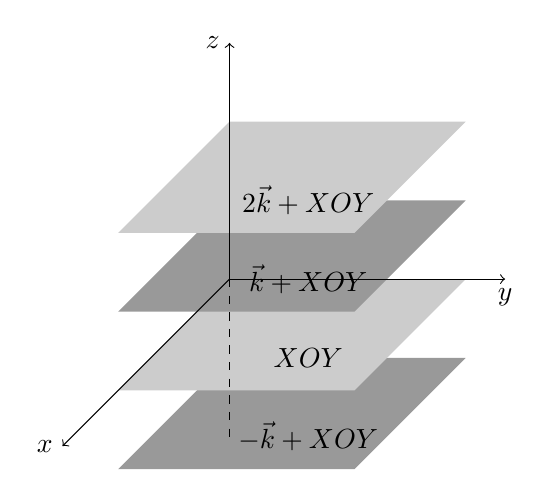
\begin{tikzpicture}
	\fill[black!40] (0,-1)--(3,-1)--({3-sqrt(2)},{-1-sqrt(2)})--({-sqrt(2)},{-1-sqrt(2)})--(0,-1) node[black] at (1,-2) {$-\vec{k}+XOY$};
	
	\fill[black!20] (0,0)--(3,0)--({3-sqrt(2)},{-sqrt(2)})--({-sqrt(2)},{-sqrt(2)})--(0,0) node[black] at (1,-1) {$XOY$};
	
	\fill[black!40] (0,1)--(3,1)--({3-sqrt(2)},{1-sqrt(2)})--({-sqrt(2)},{1-sqrt(2)})--(0,1) node[black] at (1,0) {$\vec{k}+ XOY$};
	
	\fill[black!20] (0,2)--(3,2)--({3-sqrt(2)},{2-sqrt(2)})--({-sqrt(2)},{2-sqrt(2)})--(0,2) node[black] at (1,1) {$2\vec{k}+ XOY$};
	
	\draw[dashed] (0,0)--(0,-2);
	\draw[->] (0,0)--(3.5,0) node[anchor = north] {$y$};
	\draw[->] (0,0)--(0,3) node[anchor = east] {$z$};
	\draw[->] (0,0)--({-1.5*sqrt(2)},{-1.5*sqrt(2)}) node[anchor = east] {$x$};
	\end{tikzpicture}
	\caption*{Кожна площина означає суміжний клас. Ми факторизували по $XOY$ --- і вийшло таке розбиття.}
	\end{figure}
	\end{example}

	\begin{theorem}
	Нехай $L$ --- лінійний простір та $M$ --- його підпростір. Тоді 
	\begin{align*}
	\dim M + \dim L/_{M} = \dim L.
	\end{align*}
	\end{theorem}
	
	\begin{proof}
	Нехай $\{f_1,\dots,f_n\}$ --- базис $M$. Розширимо його до $\{f_1,\dots,f_n,g_1,\dots,g_k\}$ --- базису $L$. Доведемо, що $\{g_1+W,\dots,g_k+W\}$ --- базис $L/_{M}$.
	\begin{enumerate}[wide=0pt,label={\Roman*.}]
	\item \textit{Система --- л.н.з.}\\
	Нехай маємо
	\[
	\alpha_1 (g_1+W) + \dots + \alpha_k (g_k+W) = 0+W.
	\]
	Знаючи, як облаштовані операції на факторпросторі, одержимо
	\[
	(\alpha_1g_1+\dots+\alpha_kg_k)+W = W.
	\]
	Дана рівність означає, що
	\[
	\alpha_1g_1 + \dots + \alpha_k g_k \sim 0 \implies \alpha_1g_1 + \dots + \alpha_k g_k \in M.
	\]
	Тоді розкладемо в лінійну комбінацію $f_1,\dots,f_n$:
	\[
	\alpha_1 g_1 + \dots + \alpha_k g_k = \beta_1 f_1 + \dots + \beta_n f_n.
	\]
	Але тоді за базисом $L$ одержимо
	\[
	\beta_1 f_1 + \dots + \beta_n f_n - \alpha_1 g_1 - \dots - \alpha_k g_k = 0 \implies \beta_1 = \dots = \beta_n = \alpha_1 = \dots = \alpha_k = 0.
	\]
	Таким чином, $\{g_1+W,\dots,g_k+W\}$ --- л.н.з. система.
	
	\item \textit{Розклад --- єдиний.}\\
	Тепер нехай $x+M \in L/_{M}$. Оскільки $x \in L$, то звідси 
	\[
	x = \gamma_1 f_1 + \dots + \gamma_n f_n + \delta_1 g_1 + \dots + \delta_k g_k,
	\]
	причому даний розклад  --- єдиний. Маємо
	\begin{align*}
	x+M & = (\gamma_1 f_1 + \dots + \gamma_n f_n + \delta_1 g_1 + \dots + \delta_k g_k)+M \\
	& = ((\gamma_1 f_1) + M) + \dots + ((\gamma_n f_n) + M) + ((\delta_1 g_1) + M) + \dots + ((\delta_k g_k) + M) \\ 
	& = \gamma_1 (f_1 + M) + \dots + \gamma_n (f_n+M) + \delta_1 (g_1 + M) + \dots + \delta_k (g_k + M) \overset{f_1,\dots,f_n \in M}{=} \\ & = (0+M) + \dots + (0+M) + \delta_1 (g_1+M) + \dots + \delta_k (g_k+M) = \delta_1 (g_1+M) + \dots + \delta_k (g_k+M).
	\end{align*} 
	Причому цей розклад буде єдиним.
	\end{enumerate}
	Таким чином, $\{g_1+W,\dots,g_k+W\}$ --- базис. Тобто 
	\[
	\dim L/_{M} = k = (n+k) - n = \dim L - \dim M. \qedhere
	\]
	\end{proof}
	\newpage	
	
% \fi
% Лінійні простори
	

% Дії з лінійними просторами (part 1)
%\iffalse
	\section{Дії з лінійними просторами}
	\subsection{Лінійні оператори}
	\begin{definition}
	Нехай $L,M$ --- лінійні простори.\\
	Відображення $A \colon L \to M$ називається \textbf{лінійним оператором}, якщо виконані такі умови:
	\begin{align*}
	\begin{tabular}{cl}
	1) & $\forall x_1,x_2 \in L: A(x_1+x_2)=Ax_1+Ax_2$;\\
	2) & $\forall \lambda \in \mathbb{R}: A(\lambda x) = \lambda Ax$.
	\end{tabular}
	\end{align*}
	\end{definition}
	
	\begin{proposition}[Властивості лінійних операторів]
	Нехай $L,M$ --- лінійні простори та $A \colon L \to M$ --- відображення. Тоді:
	\begin{enumerate}[nosep, wide=0pt, label={\arabic*)}]
	\item Якщо $A$ --- лінійний оператор, то $A(0) = 0$;
	\item $A$ --- лінійний оператор $\iff \forall x_1,x_2 \in L: \forall \alpha_1, \alpha_2 \in \mathbb{R}: A(\alpha_1 x_1 + \alpha_2 x_2) = \alpha_1 Ax_1 + \alpha_2 Ax_2$;
	\item Якщо $A$ --- лінійний оператор, то $\forall x_1,\dots, x_n \in L: \forall \alpha_1, \dots, \alpha_n \in \mathbb{R}: \\ A(\alpha_1 x_1 + \dots + \alpha_n x_n) = \alpha_1 Ax_1 + \dots + \alpha_n Ax_n$.
	\end{enumerate}
	\end{proposition}
	
	\begin{proof}
	%\nospacebeforeitem
	\begin{enumerate}[topsep=0cm, wide=0pt, label={\arabic*)}]
	\item Просто зауважимо, що в силу лінійності справедливий ланцюг рівностей:
	\[
	A(0) = A(x - x) = Ax + A(-x) = Ax - Ax = 0.
	\]
	
	\item Доведення буде в обидві боки.\\
	\rightproof Дано: $A$ --- лінійний оператор. Нехай $x_1,x_2 \in L$ та $\alpha_1,\alpha_2 \in \mathbb{R}$. Тоді
	\[
	A(\alpha_1 x_1 + \alpha_2 x_2) = A(\alpha_1 x_1) + A(\alpha_2 x_2) = \alpha_1 Ax_1 + \alpha_2 Ax_2.
	\]
	\leftproof Дано: $\forall x_1,x_2 \in L: \forall \alpha_1, \alpha_2 \in \mathbb{R}: A(\alpha_1 x_1 + \alpha_2 x_2) = \alpha_1 Ax_1 + \alpha_2 Ax_2$. Треба перевірити із означення два пункти.
	\begin{enumerate}[nosep,wide=0pt,label={\arabic*))}]
	\item Нехай $x_1,x_2 \in L$. Тоді якщо взяти $\alpha_1 = \alpha_2 = 1$, то одержимо наступне:
	\[
	A(x_1 + x_2) = A(1 \cdot x_1 + 1 \cdot x_2) = 1 \cdot Ax_1 + 1 \cdot Ax_2 = Ax_1 + Ax_2
	\]
	\item Нехай $x_1 \in L$ та $\alpha \in \mathbb{R}$. Тоді якщо взяти $\alpha_1 = \alpha,\ \alpha_2 = 0$, то одержимо наступне:
	\[
	A(\alpha x_1) = A(\alpha_1 x_1 + \alpha_2 x_2) = \alpha_1 A x_1 + \alpha_2 A x_2 = \alpha A x_1. \qedhere
	\]
	\end{enumerate}
	\end{enumerate}
	\end{proof}
	
	\begin{example}
	Нехай задано оператор $A \colon \underset{\substack{\rotatebox{90}{$=$} \\ L}}{\mathbb{R}^2} \to \underset{\substack{\rotatebox{90}{$=$} \\ M}}{\mathbb{R}^2}$, де
	\[
	 A\vec{x} = \begin{pmatrix} x_1 - 2x_2 \\ 3x_2 + x_1 \end{pmatrix}.
	 \]
	Перевіримо, що такий оператор є лінійним. Спершу маємо
	\[
	\vec{x} = \begin{pmatrix} x_1 \\ x_2 \end{pmatrix},\ \vec{y} = \begin{pmatrix} y_1 \\ y_2 \end{pmatrix} \implies \vec{x} + \vec{y} = \begin{pmatrix}
	x_1 + y_1 \\ x_2 + y_2
	\end{pmatrix},\qquad \alpha \vec{x} = \begin{pmatrix} \alpha x_1 \\ \alpha x_2 \end{pmatrix}.
	\]
	Якщо підставити їх, то одержимо такий ланцюг рівностей:
	\begin{align*}
	A(\vec{x} + \vec{y}) & = \begin{pmatrix} (x_1+y_1)-2(x_2+y_2) \\ 3(x_2+y_2)+(x_1+y_1) \end{pmatrix} = \begin{pmatrix} (x_1-2x_2) + (y_1-2y_2) \\ (3x_2+x_1) + (3y_2+y_1) \end{pmatrix} 
	\\& = \begin{pmatrix} x_1 - 2x_2 \\ 3x_2 + x_1 \end{pmatrix} + \begin{pmatrix} y_1 - 2y_2 \\ 3y_2 + y_1 \end{pmatrix} = A\vec{x} + A\vec{y}. \\
	A(\alpha \vec{x}) & = \begin{pmatrix} (\alpha x_1) - 2(\alpha x_2) \\ 3(\alpha x_2) + (\alpha x_1) \end{pmatrix} = \alpha \begin{pmatrix} x_1 - 2x_2 \\ 3x_2 + x_1 \end{pmatrix} = \alpha A\vec{x}.
	\end{align*}
	Отже, $A$ --- лінійний оператор.
	\end{example}
	
	\begin{example}
	Нехай задано оператор $A \colon \underset{\substack{\rotatebox{90}{$=$} \\ L}}{\mathbb{R}_n[t]} \to \underset{\substack{\rotatebox{90}{$=$} \\ M}}{\mathbb{R}_n[t]}$ так, що 
	\[
	(Af)(t) = f(t+1) - g(t),\qquad g \not\equiv 0.
	\] 
	Даний оператор уже НЕ буде лінійним, оскільки
	\[
	(A0)(x) = 0(t+1) - g(t) \equiv -g(t) \not\equiv 0.
	\]
	\end{example}
	
	\begin{definition}
	Нехай $L$ --- лінійний простір. Лінійний оператор
	\begin{align*}
	\varphi \colon L \to \mathbb{R}
	\end{align*}
	ще називають \textbf{лінійним функціоналом}.
	\end{definition}
	
	\begin{example}
	Зокрема маємо лінійний функціонал $\varphi \colon \underset{\substack{\rotatebox{90}{$=$} \\ L}}{\mathbb{R}^4} \to \mathbb{R}$, що задається як 
	\[
	\varphi(\vec{x}) = x_1 + 3x_2 - \pi x_3 + \sqrt{17}\,x_4.
	\]
	\end{example}
	
	\subsection{Арифметичні дії з лінійними операторами}
	\begin{definition}
	Нехай $A,B \colon L \to M$ --- лінійні оператори.\\
	\textbf{Сумою} лінійних операторів $A,B$ називають відображення $A+B \colon L \to M$, яке задається правилом:
	\begin{align*}
	\forall x \in L: (A+B)x = Ax+Bx.
	\end{align*}
	\textbf{Множення константи} на лінійний оператор $A$ називають відображення $\alpha A \colon L \to M$, яке задається правилом:
	\begin{align*}
	\forall x \in L: (\alpha A)(x) = \alpha (Ax).
	\end{align*}
	\end{definition}
	
	\begin{definition}
	\textbf{Одиничним оператором} назвемо оператор $I \colon L \to L$, що задається ось так:
	\begin{align*}
	\forall x \in L: Ix = x.
	\end{align*}
	\end{definition}
	
	\begin{definition}
	\textbf{Нулевим оператором} назвемо оператор $O \colon L \to M$, що задається ось так:
	\begin{align*}
	\forall x \in L: Ox = 0.
	\end{align*}
	\end{definition}
	
	\begin{lemma}
	Якщо $A,B \colon L \to M$ --- лінійні оператори, то $A+B,\ \alpha A$ --- лінійні оператори.
	\end{lemma}
	
	\begin{proof}
	\begin{enumerate}[topsep=0pt,wide=0pt,label={\Roman*.}]
	\item \textit{$A+B$ --- лінійний оператор}.\\
	Нехай $x_1,x_2 \in L$, а також $\alpha,\beta \in \mathbb{R}$. Тоді
	\begin{align*}
	(A+B)(\alpha x_1 + \beta x_2) & = A (\alpha x_1 + \beta x_2) + B (\alpha x_1 + \beta x_2) = (\alpha Ax_1 + \beta Ax_2) + (\alpha Bx_1 + \beta Bx_2) \\
	& = \alpha (Ax_1 + B x_1) + \beta(Ax_2 + Bx_2) = \alpha (A+B)(x_1) + \beta (A+B)(x_2).
	\end{align*}
	Отже, $A+B$ --- лінійний, за еквівалентним означенням.
	
	\item \textit{$\lambda A$ --- лінійний оператор}.\\
	Нехай $x_1,x_2 \in L$, а також $\alpha,\beta \in \mathbb{R}$. Тоді
	\begin{align*}
	(\lambda A)(\alpha x_1 + \beta x_2) = \lambda A(\alpha x_1 + \beta x_2) = \lambda (\alpha Ax_1 + \beta A x_2) = \alpha (\lambda A)(x_1) + \beta (\lambda A)(x_2).
	\end{align*}
	Отже, $\lambda A$ --- лінійний, за еквівалентним означенням. \qedhere
	\end{enumerate}
	\end{proof}
	
	\begin{remark}
	Одиничний оператор $I$ цілком зрозуміло, що теж лінійний оператор.
	\end{remark}
	
	\textit{Позначення}: $\mathcal{L}(L,M)$ --- множина всіх лінійних операторів. Якщо простори однакові, то ми позначаємо часто $\mathcal{L}(L,L) = \mathcal{L}(L)$.
	 
	\begin{proposition}
	$\mathcal{L}(L,M)$ буде лінійним простором із визначеними операціями $+$ (\textit{додаванням}) та $\cdot \alpha$ (\textit{множенням на скаляр}).\\
	\textit{Вправа: перевірити 8 аксіом.}
	\end{proposition}
	
	\begin{proposition}
	\label{dimension_of_space_of_linear_operators}
	Нехай $L,M$ --- векторні простори, причому $\dim L = n,\ \dim M = m$. Тоді
	\begin{align*}
	\dim \mathcal{L}(M,N) = \dim L \cdot \dim M.
	\end{align*}
	Зокрема якщо $\{x_1,\dots,x_n\}$ --- базис $L$ та $\{y_1,\dots,y_m\}$ --- базис $M$, то базисом простору $\mathcal{L}(L,M)$ буде набір операторів $\{E_{ij} \mid i = 1,\dots,m,\ j = 1,\dots,n\}$, які задаються таким чином:
	\begin{align*}
	E_{ij}(x_k) = \begin{cases} y_i, & j = k; \\ 0, & j \neq k. \end{cases}
	\end{align*}
	\end{proposition}
	
	\begin{proof}
	\begin{enumerate}[wide=0pt,topsep=0pt,label={\Roman*.}]
	\item \textit{Система -- л.н.з.}\\
	Припустимо, що
	\[
	\alpha_{11} E_{11} + \dots + \alpha_{1n} E_{1n} + \dots + \alpha_{m1} E_{m1} + \dots + \alpha_{mn} E_{mn} \equiv O.
	\]
	Підставимо $x_k$ в ліву частину --- отримаємо рівність 
	\[
	\alpha_{1k} y_1 + \dots + \alpha_{mk} y_m = 0.
	\] 
	Проте оскільки $\{y_1,\dots,y_m\}$ --- л.н.з., то звідси $\alpha_{ik} = 0, i = 1,\dots,m$. Це все виконується для кожного $k$, тому звідси $\alpha_{ij} = 0, i = 1,\dots,m,\ j = 1,\dots,n$.
	
	\item \textit{Система --- повна.}\\
	Нехай $A \in \mathcal{L}(M,N)$. Для кожного $z \in L$ маємо 
	\[
	z = \beta_1 x_1 + \dots + \beta_n x_n.
	\]
	Подіявши оператором $A$, одержимо
	\[
	Az = \beta_1 Ax_1 + \dots + \beta_n Ax_n.
	\]
	Кожний елемент $\beta_j A x_j \in M$, тому розкладемо за базисом 
	\[
	\beta_j Ax_j = \beta_j \gamma_{1j} y_1 + \dots + \beta_j \gamma_{mj} y_m.
	\]
	Тепер зауважимо, що
	\begin{align*}
	E_{1j}(z) = \beta_1 E_{j1}(x_1) + \dots + \beta_n E_{1j}(x_n) = \beta_j y_1; \\
	\vdots \\
	E_{mj}(z) = \beta_1 E_{mj}(x_1) + \dots + \beta_n E_{mj}(x_n) = \beta_j y_m.
	\end{align*}
	Тобто 
	\[
	\beta_j Ax_j = \gamma_{1j} E_{1j} z + \dots + \gamma_{mj} E_{mj} z.
	\]
	Це означатиме, що справджується рівність:
	\[
	Az = (\gamma_{11} E_{11} z + \dots + \gamma_{m1} E_{m1}z) + \dots + (\gamma_{1n} E_{1n}z + \dots + \gamma_{mn} E_{mn}z).
	\]
	Дана рівність виконується при всіх можливих $z \in L$. Скаляри $\gamma_{ij}$ не залежать від $z$. Отже,
	\[
	A \equiv \gamma E_{11} + \dots + \gamma_{m1} E_{m1} + \dots + \gamma_{1n} E_{n1} + \dots + \gamma_{mn} E_{mn}. \qedhere
	\]
	\end{enumerate}
	\end{proof}
	
	\begin{definition}
	\textbf{Дельта-символ Кронекера} визначається ось так:
\begin{align*}
\delta_{ij} = \begin{cases} 1, & i = j; \\ 0, & i \neq j. \end{cases} 
\end{align*}
	\end{definition}
	
	\begin{remark}
	Отже, для оператора $E_{ij}$ можна записати компактну рівність:
	\begin{align*}
	E_{ij}x_k = y_i \delta_{jk}.
	\end{align*}
	\end{remark}
	
	\begin{definition}
	Нехай $A \in \mathcal{L}(L,M)$ та $B \in \mathcal{L}(M,N)$.\\
	\textbf{Добутком} операторів $A,B$ називають відображення $BA \colon L \to N$, яке визначено правилом:
	\begin{align*}
	\forall x \in L: (BA)x = B(Ax).
	\end{align*}
	\end{definition}
	
	\begin{lemma}
	Якщо $A \in \mathcal{L}(L,M)$ та $B \in \mathcal{L}(M,N)$, то $BA \in \mathcal{L}(L,N)$.
	\end{lemma}
	
	\begin{proof}
	Нехай $x_1,x_2 \in L$, а також $\alpha,\beta \in \mathbb{R}$, тоді:
	\begin{align*}
	(BA)(\alpha x_1 + \beta x_2) & = B(A(\alpha x_1 + \beta x_2)) = B(\alpha Ax_1 + \beta Ax_2) = \alpha B(A(x_1)) + \beta B(A(x_2)) \\
	& = \alpha (BA)(x_1) + \beta (BA)(x_2).
	\end{align*}
	Отже, $BA$ --- дійсно лінійний оператор за еківалентним означенням.
	\end{proof}
	
	\begin{remark}
	Якщо $A,B \colon L \to L$, то взагалі-то кажучи $BA \neq AB$.
	\end{remark}
	
	\begin{example}
	Зокрема задамо лінійні оператори $A \colon \mathbb{R}^2 \to \mathbb{R}^2,\ B \colon \mathbb{R}^2 \to \mathbb{R}^2$ таким чином:
	\begin{align*}
	A \vec{x} = \begin{pmatrix}
	2x_1 + x_2 \\ 3x_1 + x_2
	\end{pmatrix}, \qquad B\vec{x} = \begin{pmatrix}
	-x_1 \\ x_1 + x_2
	\end{pmatrix}.
	\end{align*}
	Обчислимо в кожному випадку композицію:
	\begin{align*}
	BA \vec{x} = B \begin{pmatrix}
	2x_1 + x_2 \\ 3x_1 + x_2
	\end{pmatrix} = \begin{pmatrix}
	-2x_1-x_2 \\ 2x_1+x_2+3x_1+x_2
	\end{pmatrix} = \begin{pmatrix}
	-2x_1-x_2 \\ 5x_1+2x_2
	\end{pmatrix}, \\
	AB \vec{x} = A \begin{pmatrix}
	-x_1 \\ x_1 + x_2
	\end{pmatrix} = \begin{pmatrix}
	-2x_1 + x_1 + x_2 \\ -3x_1 + x_1 + x_2
	\end{pmatrix} = \begin{pmatrix}
	-x_1 + x_2 \\ -2x_1 + x_2
	\end{pmatrix}.
	\end{align*}
	У цьому випадку зрозуміло, що $BA \not\equiv AB$.
	\end{example}
	
	\begin{theorem}[Властивості добутку лінійних операторів]
	Нехай $A,B,C \in \mathcal{L}(L,L)\footnote{Насправді, тут і деяких інших твердженнях нижче зовсім не обов'язково вимагати лінійність оператора, але оскільки вчимо лінійну алгебру, то зосередимось саме на них.}$. Тоді:
	\begin{enumerate}[nosep, wide=0pt, label={\arabic*)}]
	\item $(A \cdot B) \cdot C = A \cdot (B \cdot C)$;
	\item $A \cdot I = I \cdot A$;
	\item $A \cdot (B+C) = A \cdot B + A \cdot C, \qquad (A+B) \cdot C = A \cdot C + B \cdot C$.
	\end{enumerate}
	\end{theorem}
	
	\begin{proof}
	\begin{enumerate}[nosep, wide=0pt, label={\arabic*)}]
	\item Із одного боку,
	\[
	((A \cdot B) \cdot C) x = (A \cdot B) \cdot (Cx) = A \cdot (B \cdot (Cx)).
	\]
	Водночас з іншого боку,
	\[
	(A \cdot (B \cdot C)) x = A \cdot ( (B \cdot C) x) = A \cdot (B \cdot (Cx)).
	\]
	
	\item Маємо відносно простий ланцюг рівностей:
	\[
	(A \cdot I) x = A \cdot (Ix) = A x = I \cdot (A x) = (I \cdot A) x.
	\]

	\item Спочатку доводиться перша рівність:
	\[
	[A \cdot (B + C)]x = A \cdot [(B+C)x] = A \cdot (Bx + Cx) = A (Bx) + A (Cx) = (A \cdot B)x + (A \cdot C)x = (A \cdot B + A \cdot C)x.
	\]
	Тепер схожим чином доводиться друга рівність:
	\[
	[(A+B) \cdot C]x = (A+B) \cdot (Cx) = A (Cx) + B (Cx) = (A \cdot C)x + (B \cdot C)x = (A \cdot C + B \cdot C)x. \qedhere
	\]
	\end{enumerate}
	\end{proof}
	
	(\textit{наступне зауваження для тих, хто вчив абстрактну алгебру, зокрема теорію кілець.})
	
	\begin{remark}
	Множина $\mathcal{L}(L,L)$ є кільцем з одиницею. Тому що $\mathcal{L}(L,L)$ --- лінійний простір, а тому утворює абелеву групу, а також існує операція множення, для якої виконуються властивості вище, які є аксіомами для кільця.
	\end{remark}
	
	\subsection{Ядро, образ оператора}	
	\begin{definition}
	Нехай $A \in \mathcal{L}(L,M)$.\\
	\textbf{Ядром} оператора $A$ називають таку множину:
	\begin{align*}
	\ker A = \{x \in L: Ax = 0\} \overset{\text{якщо коротко}}{=} A^{-1}(0).
	\end{align*}
	\textbf{Образом} оператора $A$ називають таку множину:
	\begin{align*}
	\Im A = \{y \in M: \exists x \in L: y = Ax\} \overset{\text{якщо коротко}}{=} A(L).
	\end{align*}
	\end{definition}
	
	\begin{theorem}
	Нехай $A \in \mathcal{L}(L,M)$. Тоді $\ker A$ та $\Im A$ --- підпростори відповідно лінійним просторам $L$ та $M$.
	\end{theorem}
	
	\begin{proof}
	\begin{enumerate}[topsep=0pt, wide=0pt,label={\Roman*.}]
	\item \textit{$\ker A$ --- підпростір $L$}.\\
	Дійсно, нехай $x_1,x_2 \in \ker A$. Тоді
	\[
	A(x_1+x_2)=Ax_1+Ax_2 = 0 + 0 = 0 \implies x_1+x_2 \in \ker A.
	\]
	Також якщо обрати $\lambda \in \mathbb{R}$, то отримаємо
	\[
	A(\lambda x_1) = \lambda Ax_1 = 0 \implies \lambda x_1 \in \ker A.
	\]
		
	\item \textit{$\Im A$ --- підпростір $M$}.\\
	Нехай $y_1,y_2 \in \Im A$, тобто $y_1 = Ax_1,\ y_2 = Ax_2$ для деяких $x_1,x_2 \in L$. Тоді
	\[
	y_1 + y_2 = Ax_1 + Ax_2 = A(x_1+x_2) \implies y_1+y_2 \in \Im A.
	\]
	Також якщо обрати $\lambda \in \mathbb{R}$, то отримаємо
	\[
		\lambda y_1 = \lambda Ax_1 = A(\lambda x_1) \implies \lambda y_1 \in \Im A. \qedhere
	\]
	\end{enumerate}
	\end{proof}
	
	\begin{example}
	Нехай оператор $A \colon \mathbb{R}_n[x] \to \mathbb{R}_n[x]$ задається формулою: 
	\[
	(Af)(x) = f'(x).
	\]
	(\textit{вправа: довести, що $A \in \mathcal{L}(\mathbb{R}_n[x])$}). Знайдемо ядро та образ даного оператора.
	\[
	f \in \ker A \implies (Af)(x) = 0 \implies f'(x) \equiv 0 \implies f(x) = const.
	\]
	Отже, $\ker A = \{ f(x) = const\} \overset{\textrm{або}}{=} \mathbb{R}_0[x]$.
	\[
	g \in \Im A \implies \exists f: g(f) = (Af)(x) \implies g(x) = f'(x).
	\]
	Отже, $\Im A = \mathbb{R}_{n-1}[x]$.
	\end{example}

\noindent
	Образ не завжди легко шукати, тому дамо ще кілька важливих тверджень для спрощення пошуку.
	\begin{lemma}[Структура образа]
	Нехай $A \in \mathcal{L}(L,M)$ та $\{e_1,\dots, e_n\}$ --- базис простору $L$. Тоді 
	\[
	\Im A = \linspan \{Ae_1,\dots, Ae_n\}.
	\]
	(\textit{не факт, що всі вектори тут лінійно незалежні, але Бог з ними}.)
	\end{lemma}
	
	\begin{proof}
	Нехай $y \in \Im A$, тобто $y = Ax$ для деякого $x \in L$. Тоді маємо:
	\[
	y = Ax \overset{\textrm{за базисом}}{=} A(x_1e_1 + \dots + x_n e_n) = x_1 Ae_1 + \dots + x_n A e_n \implies y \in \linspan\{Ae_1,\dots,Ae_n\}.
	\]
	Нехай тепер $y \in \linspan\{Ae_1,\dots,Ae_n\}$. Тоді 
	\[
	y = \alpha_1 Ae_1 + \dots + \alpha_n Ae_n = A(\alpha_1 e_1 + \dots + \alpha_n e_n).
	\] 
	Якщо позначити $x = \alpha_1 e_1 + \dots + \alpha_n e_n$, то тоді $y = Ax$, тобто $y \in \Im A$.\\
	Отже, $\Im A = \linspan \{Ae_1, \dots, Ae_n \}$.
	\end{proof}
	
	\begin{theorem}[Зв'язок розмірностей ядра та образа]
	Нехай $A \in \mathcal{L}(L,M)$ та $L$ --- скінченно вимірний \textit{(!)} простір. Тоді
	\begin{align*}
	\dim \ker A + \dim \Im A = \dim L.
	\end{align*}
	\end{theorem}
	
	\begin{proof}
	Нехай $\{f_1, \dots, f_n\}$ --- базис $\ker A$ та $\{g_1, \dots, g_m\}$ --- базис $\Im A$. У нас тут $\dim \ker A = n, \dim \Im A = m$. Одразу запишемо, що $g_j = Ah_j$ для деяких $h_j \in L$. Перевіримо, що 
	\[
	\{f_1,\dots, f_n, h_1,\dots, h_m\}
	\]
	утворюватиме базис простору $L$.
	
	\begin{enumerate}[wide=0pt,label={\Roman*.}]
	\item \textit{Система -- л.н.з.}\\
	Нехай
	\[
	\alpha_1 f_1 + \dots + \alpha_n f_n + \beta_1 h_1 + \dots + \beta_m h_m = 0.
	\]
	Подіємо оператором $A$ на цю лінійну комбінацію --- зрештою отримаємо
	\[
	\alpha_1 Af_1 + \dots + \alpha_n Af_n + \beta_1 Ah_1 + \dots + \beta_m A h_m = 0.
	\]
	Знаючи, що $f_i \in \ker A$, перепишемо як
	\[
	0 + \dots + 0 + \beta_1 g_1 + \dots + \beta_n g_n = 0 \overset{\textrm{базис}}{\implies} \beta_1 = \dots = \beta_n = 0.
	\]
	Підставимо отримані $\beta$ в найперше рівняння:
	\[
	\alpha_1 f_1 + \dots + \alpha_n f_n = 0 \overset{\textrm{базис}}{\implies} \alpha_1 = \dots = \alpha_n = 0.
	\]
	Отже, з наших міркувань $\alpha_1 = \dots = \alpha_n = \beta_1 = \dots = \beta_n = 0$. Таким чином, довели л.н.з.
	
	\item \textit{Система -- повна.}\\
	Оберемо $z \in L$, тоді оскільки $Az \in \Im A$, то
	\[
	Az = \gamma_1 g_1 + \dots + \gamma_m g_m.
	\]
	Розглянемо елемент $w \in L$, який задається формулою: 
	\[
	w = z - (\gamma_1 h_1 + \dots + \gamma_m h_m).
	\]
	Ідейно підбирали таке $w$, щоб $w \in \ker A$. І справді,
	\[
	Aw = A(z - (\gamma_1 h_1 + \dots + \gamma_m h_m)) = Az - \gamma_1 Ah_1 - \dots - \gamma_m Ah_m = Az - \gamma_1 g_1 - \dots - \gamma_m g_m = 0 \implies w \in \ker A.
	\]
	Оскільки $w \in \ker A$, то розкладемо за базисом:
	\[
	w = \tau_1 f_1 + \dots + \tau_n f_n.
	\] 
	Отримали в результаті ось таке:
	\[
	\tau_1 f_1 + \dots + \tau_n f_n = z - (\gamma_1 h_1 + \dots + \gamma_m h_m) \implies z = \tau_1 f_1 + \dots + \tau_n f_n + \gamma_1 h_1 + \dots + \gamma_m h_m.
	\]
	Таким чином, маємо повну систему.
	\end{enumerate}
	
	Разом отримали, що $\{f_1,\dots, f_n, h_1,\dots, h_m\}$ --- базис $L$, а отже
	\[
	\dim L = m+n  \implies \dim L = \dim \ker A + \dim \Im A. \qedhere
	\]
	\end{proof}

	Часто можна зустріти таку термінологію про $\dim \Im A$ та $\dim \ker A$, запишу означення.
	
	\begin{definition}
Нехай $A \in \mathcal{L}(L,M)$ та $L$ --- скінченно вимірний.\\
\textbf{Рангом} оператора $A$ називають розмірність образа оператора:
\begin{align*}
\rank A = \dim \Im A.
\end{align*}
\textbf{Дефектом} оператора $A$ називають розмірність ядра оператора:
\begin{align*}
\defect A = \dim{\ker A}.
\end{align*}
	\end{definition}
	
	\begin{example}
	Задамо лінійний оператор $A \colon \mathbb{R}^3 \to \mathbb{R}^3$ ось так:
	\[
	A \vec{x} = \begin{pmatrix}
	x_1 - x_2 + x_3 \\
	2x_1 + x_2 - 3x_3 \\
	x_1 + 2x_2 - 4x_3
	\end{pmatrix}.
	\]
	Знайдемо ядро та образ даного оператора.
	\begin{align*}
	\vec{x} \in \ker A \iff A\vec{x} = \vec{0} & \iff \begin{cases} x_1 - x_2 + x_3 = 0; \\ 2x_1 + x_2 - 3x_3 = 0; \\ x_1 + 2x_2 - 4x_3 = 0. \end{cases} \iff \begin{cases} x_1 - x_2 + x_3 = 0; \\ 3x_2 - 5x_3 = 0. \end{cases} \\
	& \iff \begin{cases} x_1 = \dfrac{2}{3}x_3; \\ x_2 = \dfrac{5}{3}x_3. \end{cases} \iff \vec{x} = \begin{pmatrix} \dfrac{2}{3}x_3 \\ \dfrac{5}{3}x_3 \\ x_3  \end{pmatrix} = \dfrac{1}{3}x_3 \begin{pmatrix} 2 \\ 5 \\ 3 \end{pmatrix}.
	\end{align*}
	Отже, ми одержали структуру ядра:
	\[
	\ker A = \linspan \left\{\begin{pmatrix} 2 \\ 5 \\ 3 \end{pmatrix} \right\}.
	\]
	\bigskip \\
	Зафіксуємо базис $\{\vec{e}_1, \vec{e}_2, \vec{e}_3\}$, де всюди одиничні вектори. Звідси 
	\[
	A \vec{e}_1 = \begin{pmatrix}
	1 \\ 2 \\ 1
	\end{pmatrix},\quad A \vec{e}_2 = \begin{pmatrix}
	-1 \\ 1 \\ 2
	\end{pmatrix},\quad A \vec{e}_3 = \begin{pmatrix}
	1 \\ -3 \\ -4
	\end{pmatrix}.
	\]
	Тоді за лемою ми насправді маємо структуру образа 
	\[
	\Im A = \linspan \left\{ \begin{pmatrix} 1 \\ 2 \\ 1 \end{pmatrix}, \begin{pmatrix} -1 \\ 1 \\ 2 \end{pmatrix}, \begin{pmatrix} 1 \\ -3 \\ -4 \end{pmatrix} \right\}.
	\]
	Однак відомо, що $\dim \Im A = \dim \mathbb{R}^3 - \dim \ker A = 2$. Тоді варто писати 
	\[
	\Im A = \linspan \left\{ \begin{pmatrix} 1 \\ 2 \\ 1 \end{pmatrix}, \begin{pmatrix} -1 \\ 1 \\ 2 \end{pmatrix} \right\}.
	\]
	\end{example}
	\noindent
	Завдяки ядру та образу ми можемо описати відображення на сюр'єктивність чи ін'єктивність.
	\begin{proposition}
	\label{one-to-one_criterion}
	Нехай $A \in \mathcal{L}(L,M)$. Тоді
	\begin{center}
	$A$ --- ін'єктивний оператор $\iff \ker A = \{0\}$.
	\end{center}
	\end{proposition}
	
	\begin{proof}
	\rightproof Дано: $A$ --- ін'єктивний. Нехай $x \in \ker A$, тоді звідси $Ax = 0 = A0$. За ін'єктивністю $x = 0$. Отже, $\ker A = \{0\}$.
	\bigskip \\
	\leftproof Дано: $\ker A = \{0\}$. Нехай виконується $Ax = Ay$, тоді звідси $A(x-y) = Ax - Ay = 0$, тобто $x-y \in \ker A \implies x - y = 0$. Таким чином, $x = y$, а тому $A$ --- ін'єктивний.
	\end{proof}
	
	\begin{proposition}
	\label{onto_criterion}
	Нехай $A \in \mathcal{L}(L,M)$. Тоді
	\begin{center}
	$A$ --- сюр'єктивний оператор $\iff \Im A = M$.
	\end{center}
	\textit{Вправа: довести.}
	\end{proposition}

\iffalse
	\begin{proof}
	\rightproof Дано: $A$ --- сюр'єктивний оператор. За означення образа $\Im A \subset M$. Тепер нехай $y \in M$, тоді за сюр'єктивністю, $\exists x \in L: y = Ax$, тоді звідси $y \in \Im A$. Отже, $M \subset \Im A$. А тому $\Im A = M$.
	\bigskip \\
	\leftproof Дано: $\Im A = M$, тобто звідси $\forall y \in M: \exists x \in L: y = Ax$. Отже, $A$ - сюр'єктивний.
	\end{proof}
\fi

	\subsection{Обернений оператор}
	\begin{definition}
	Нехай $A \colon L \to M$ --- деякий оператор.\\
	Оператор $A$ називають \textbf{оборотним}, якщо існує деякий оператор $B \colon M \to L$, для якого
	\begin{align*}
	\forall x \in L: BAx = x; \\
	\forall y \in M: ABy = y.
	\end{align*}
	Можна переписати умову інакше:
	\begin{align*}
	BA = I_L, \qquad I_L \colon L \to L; \\
	AB = I_M, \qquad I_M \colon M \to M.
	\end{align*}
	Водночас оператор $B$ називають \textbf{оберненим} до $A$.\\
	\textit{Позначення}: $B = A^{-1}$.
	\end{definition}
	
% Well, it's clear if study generally functions
\iffalse
	\begin{proposition}
	Задано $A \colon L \to M$ -- лінійний оборотний оператор. Тоді обернений оператор $A^{-1}$ задається єдиним чином.
	\end{proposition}
	
	\begin{proof}
	За умовою, ми маємо зворотний оператор $A_1^{-1}$.\\
	!Припустимо, що існує також $A^{-1}_2$. Тоді $\forall y \in M:$\\
	$A^{-1}_1 y = A^{-1}_1 I_M y = A^{-1}_1 A A^{-1}_2 y = (A^{-1}_1 A) (A^{-1}_2 y) = I_L (\underset{\in L}{A^{-1}_2 y}) = A_2^{-1}y$\\
	$\implies A^{-1}_1 = A^{-1}_2$. Суперечність!
	\end{proof}
\fi

%TODO look for some suitable examples
\iffalse
	\begin{example}
	Задано $A \colon \mathbb{R}_3[x] \to \Mat(2 \times 2)$ -- такий лінійний оператор:\\
	$f(x) = a + bx + cx^2 + dx^3$\\
	$(Af)(x) = \begin{pmatrix}
	a+b & a-2c \\
	d & b-d
	\end{pmatrix}$\\
	Визначимо оператор $B \colon \Mat(2 \times 2) \to \mathbb{R}_3[x]$ таким чином, що:\\
	$\mathbb{A} = \begin{pmatrix}
	a & b \\
	c & d
	\end{pmatrix}$.\\
	$B\mathbb{A} = (a-c-d) + (c+d)x + \dfrac{1}{2}(a-b-c-d)x^2 + cx^3$.\\
	Перевіримо, що $B$ -- обернений оператор зліва та справа. Справді:\\
	$\forall f \in \mathbb{R}_3[x]: (BAf)(x) = B(Af(x)) = B(A(a+bx+cx^2+dx^3))= B \begin{pmatrix}
	a+b & a-2c \\
	d & b-d
\end{pmatrix} = \\ = [a+b-d-(b-d)] + [d + (b-d)]x + \dfrac{1}{2}[(a+b)-(a-2c)-d-(b-d)]+dx^3 = a + bx + cx^2 + dx^3 = f(x)$.
\bigskip \\
$\forall \mathbb{A} \in Mat(2 \times 2): AB \mathbb{A} = A(B \mathbb{A}) = A \left( B\begin{pmatrix}
a & b \\
c & d
\end{pmatrix} \right) = A\left[(a-c-d)+(c+d)x+\dfrac{1}{2}(a-b-c-d)x^2+cx^3 \right] = \\ = \begin{pmatrix}
(a-c-d)+(c+d) & (a-c-d)-2 \dfrac{1}{2}(a-b-c-d) \\
c & (c+d)-c
\end{pmatrix} = \begin{pmatrix}
a & b \\
c & d
\end{pmatrix} = \mathbb{A}$.\\
Отримали:
$(BAf)(x) = f(x)$ та $AB \mathbb{A} = \mathbb{A}$. Отже, $B$ -- обернений оператор до $A$, або $B = A^{-1}$.
	\end{example}
\fi
	
	\begin{example}
	Нехай оператор $A \colon \mathbb{R}^2 \to \mathbb{R}^2$ задається формулою:
	\[
	A\vec{x} = \begin{pmatrix}
	x_1 + x_2 \\ 2x_1 + 2x_2
	\end{pmatrix}.
	\]
	Маємо наступне:
	\[
	A\vec{x} = \vec{y} \implies \begin{cases} x_1 + x_2 = y_1; \\ 2x_1 + 2x_2 = y_2. \end{cases}
	\]
	Відносно $x_1,x_2$ система не містить розв'язків. Отже, не існує оберненого оператора.
	\end{example}
	
	\begin{proposition}
	Якщо $A \in \mathcal{L}(L,M)$, який ще й оборотний, то $A^{-1} \in \mathcal{L}(M,L)$.
	\end{proposition}
	
	\begin{proof}
	Дійсно, нехай $y_1,y_2 \in M$ та $\alpha_1,\alpha_2 \in \mathbb{R}$. Оскільки $A$ --- оборотний, то
	\[
	y_1 = AA^{-1}y_1, \qquad y_2 = AA^{-1}y_2.
	\]
	Тоді маємо таку рівність:
	\begin{align*}
	A^{-1}(\alpha_1 y_1 + \alpha_2 y_2) & = A^{-1}(\alpha_1 AA^{-1}y_1 + \alpha_2 AA^{-1}y_2) = A^{-1}[A(\alpha_1 A^{-1}y_1 + \alpha_2 A^{-1}y_2)] \\ 
	& = A^{-1}A(\alpha_1 A^{-1}y_1 + \alpha_2 A^{-1}y_2)) = \alpha_1 A^{-1}y_1 + \alpha_2 A^{-1}y_2.
	\end{align*}
	Отже, $A^{-1}$ --- справді лінійний оператор.
	\end{proof}
	
	\begin{proposition}
	Нехай $A \colon L \to M$ --- оборотний оператор. Тоді $A^{-1} \colon M \to L$ теж є оборотним, а для її оберненого оператору справедлива рівність 
	\[
	(A^{-1})^{-1} = A.
	\]
	\end{proposition}
	
	\begin{proof}
	Якщо $A$ --- оборотний, то існує $A^{-1}$, для якого
	\[
	 AA^{-1} = I_M, \qquad A^{-1}A = I_L.
	\]
	 Ну й ба більше, цей оператор --- єдиний.\\
	Створимо якийсь обернений оператор $T \colon L \to M$, щоб 
	\[
	A^{-1}T = I_L, \qquad TA^{-1} = I_M.
	\]
	Тоді 
	\[
	I_L = A^{-1}A = A^{-1}T,\qquad I_M = AA^{-1} = TA^{-1}.
	\]
	Звідси $T = A$. Отже, $A^{-1}$ зворотний до $A = (A^{-1})^{-1}$.
	\end{proof}

%Easy
\iffalse
	\begin{lemma}
	\label{invertibility_criterion}
	Задано $A \colon L \to M$ -- лінійний оператор.\\
	$A$ -- оборотний $\iff$ $A$ -- бієктивне відображення.
	\end{lemma}
	
	\begin{proof}
	\rightproof Дано: $A$ - оборотний, тобто $\exists A^{-1}$.\\
	\textit{$A$ -- сюр'єктивне відображення.}\\
	Зафіксуємо будь-який $y \in M$. Встановимо $x = A^{-1}y$. Тоді маємо, що $Ax = AA^{1}y = y$. Отже, оператор є сюр'єктивним.\\
	\textit{$A$ -- ін'єктивне відображення.}\\
	!Припустимо, що $\forall x_1,x_2 \in L: x_1 \neq x_2 \implies Ax_1 = Ax_2$. Тоді звідси $Ax_1 - Ax_2 = A(x_1-x_2)=0=AA^{-1}0 \implies x_1 - x_2 = 0$. Суперечність! \\
	Отже, $\forall x_1,x_2 \in L: x_1 \neq x_2 \implies Ax_1 \neq Ax_2$. Тобто є ін'єктивним.\\
	Остаточно: сюр'єктивне + ін'єктивне = бієктивне.
	\bigskip \\
	\leftproof Дано: $A$ -- бієктивний, тобто $\forall y \in M: \exists! x \in L: y=  Ax$.\\
	Побудуємо оператор $B \colon M \to L$, такий, що $\forall y \in M: x = By \in L$ Тоді:\\
	$\forall y \in M: ABy = Ax = y$;\\
	$\forall x \in L: BAx = By = x$.\\
	Тому $B = A^{-1}$, а наш оператор $A$ - оборотний.
	\end{proof}
\fi
	
	\begin{proposition}[Властивості оборотних операторів]
	Нехай $A \in \mathcal{L}(L,M)$ та $B \in \mathcal{L}(M,N)$ --- оборотні оператори. Тоді:
	\begin{enumerate}[nosep, wide=0pt, label={\arabic*)}]
	\item $I^{-1} = I$;
	\item $(A \cdot B)^{-1} = B^{-1} A^{-1}$;
	\item $(\alpha A)^{-1} = \alpha^{-1} A^{-1}$.
	\end{enumerate}
	\end{proposition}
	
	\begin{proof}
	\begin{enumerate}[nosep,, wide=0pt, label={\arabic*)}]
	\item $I \cdot I^{-1} = I \cdot I = I$.
	\item $(A \cdot B) \cdot (A \cdot B)^{-1} = (A \cdot B) \cdot (B^{-1} \cdot A^{-1}) = A \cdot I \cdot A^{-1} = I$.
	\item $(\alpha A) \cdot (\alpha A)^{-1} = (\alpha A) \cdot (\alpha^{-1} A^{-1}) = \alpha A \cdot \alpha^{-1} A^{-1} = A \cdot A^{-1} = I$. \qedhere
	\end{enumerate}
	\end{proof}
	
	\begin{theorem}
	Нехай $A \in \mathcal{L}(L,M)$. Тоді
	\begin{center}
	$A$ --- оборотний $\iff$ $\begin{cases} \ker A = \{0\}; \\ \Im A = M \end{cases}.$
	\end{center}
	\textit{Випливає з того, що $A$ --- бієктивне, а згодом за \prpref{one-to-one_criterion} та \prpref{onto_criterion}.}
	\end{theorem}
	
	\begin{corollary}
	Нехай $A \in \mathcal{L}(L)$. Тоді
	\begin{center}
	$A$ --- оборотний $\iff \ker A = \{0\}$.
	\end{center}
	\textit{Вказівка: зв'язок розмірностей ядра та образа}.
	\end{corollary}
	
	\subsection{Ізоморфні лінійні простори, ізоморфізм}
	\begin{definition}
	Лінійні простори $L,\ M$ називаються \textbf{ізоморфними}, якщо
	\begin{center}
	існує бієктивний оператор $A \in \mathcal{L}(L,M)$.
	\end{center}
	\textit{Позначення}: $L \cong M$.\\
	У цьому випадоку оператор $A$ називають \textbf{ізоморфізмом}.
	\end{definition}
	
	\begin{theorem}
	Нехай $A \in \mathcal{L}(L,M)$. Тоді
	\begin{center}
	$A$ --- ізоморфізм $\iff$ якщо $\{f_1,\dots,f_n\}$ -- базис в $L$, то $\{\underset{\substack{\rotatebox{90}{$=$} \\ Af_1}}{g_1},\dots, \underset{\substack{\rotatebox{90}{$=$} \\ Af_n}}{g_n}\}$ -- базис в $M$.
	\end{center}
	\end{theorem}
	
	\begin{proof}
	\rightproof Дано: $L \cong M$, або $A \colon L \to M$ --- ізоморфізм. Також в нас відомий базис $\{f_1,\dots,f_n\}$ в $L$. Перевіримо, що $\{g_1,\dots,g_n\}$ --- базис. І дійсно, для кожного $y \in M$
	\[
	y = Ax = A(\alpha_1 f_1 + \dots + \alpha_n f_n) = \alpha_1 Af_1 + \dots + \alpha_n Af_n = \alpha_1 g_1 + \dots + \alpha_n g_n.
	\]
	Отримали розклад єдиним чином. Отже, $\{g_1,\dots,g_n\}$ --- базис в $M$.
	\bigskip \\
	\leftproof Дано: $\{f_1,\dots,f_n\},\ \{Af_1,\dots,Af_n\}$ --- відповідно базиси в $L,\ M$. Тобто маємо, що
	\[
	Ax = A(\alpha_1 f_1 + \dots + \alpha_n f_n) = \alpha_1 Af_1 + \dots + \alpha_n Af_n = y.
	\]
	Покажемо, що цей оператор є оборотним. Із щойно ''маємо'' отримали, що 
	\[
	\forall y \in M: y \in \Im A \implies M \subset \Im A.
	\]
	За означенням образа $\Im A \subset M$. Тоді $\Im A = M \implies \dim(\ker A) = 0 \implies \ker A = \{0\}$.\\
	Отже, $A$ --- оборотний оператор, а тому ізоморфізм.
	\end{proof}
	
	\begin{theorem}
	Справедливе наступне:
	\begin{center}
	$L \cong M \iff \dim L = \dim M$.
	\end{center}
	\textit{Випливає під час доведення попередньої теореми.}
	\end{theorem}
	
	\begin{corollary}
	Будь-який векторний простір розмірності $n$ ізоморфний арифметичному простору. Простіше кажучи,
	\[
	L \cong \mathbb{R}^n.
	\]
	\end{corollary}
	
	\begin{example}
	$\mathbb{R}_2[x] \cong \mathbb{R}^3$, оскільки $\dim(\mathbb{R}_2[x]) = \dim (\mathbb{R}^3) = 3$. Крім того, кожному многочлену $ax^2 + bx +c \in \mathbb{R}_2[x]$ можна однозначним чином поставити в відповідність вектор $\begin{pmatrix}
	a \\ b \\ c
	\end{pmatrix} \in \mathbb{R}^3$. 
	\end{example}
	
	\subsection{Пряма сума операторів (продовження про прямі суми)}
	\textit{Зараз поверну борг та доведу, що зовнішня та внутрішня пряма сума --- це ''одне й те саме''.}
	
	\begin{definition}
	Нехай $L_1,L_2$ --- лінійні простори.\\
	\textbf{Вкладенням} назвемо відображення $\imath_{L_1} \to L_1 \to L_1 \oplus L_2$ (\textit{на зовнішню пряму суму}), яке працює~як
	\begin{align*}
	\imath_{L_1}(x) = (x,0).
	\end{align*}
	\end{definition}
	
	\begin{remark}
	Цілком зрозуміло, що $\imath_{L_1} \in \mathcal{L}(L_1, L_1 \oplus L_2)$.
	\end{remark}
	
	\begin{proposition}
	Нехай $L_1,\ L_2$ --- лінійні простори, позначимо зовнішню пряму суму за $L = L_1 \oplus L_2$. Розглянемо підпростори
	\begin{align*}
	L_1 \oplus 0 = \{ (x,0) \mid x \in L_1 \}, \qquad 0 \oplus L_2 = \{ (0,y) \mid y \in L_2 \}.
	\end{align*}
	(\textit{вправа: довести, що воні справді підпростори $L$}). Тоді $L_1 \oplus 0 \cong L_1$ та $0 \oplus L_2 \cong L_2$, а також
	\begin{align*}
	L \cong L_1 \oplus L_2.
	\end{align*}
	Іншими словами, зовнішню пряму суму $L = L_1 \oplus L_2$ можна сприймати як внутрішню пряму суму підпросторів $L_1, L_2$ простора $L$.
	\end{proposition}
	
	\begin{proof}
	Той факт, що $L_1 \oplus 0 \cong L_1$, довести неважко, якщо довести, що відображення $\imath \colon L_1 \to 0 \oplus L_1$ (\textit{яке вже лінійне}) задає ізомомрфізм (\textit{аналогічно при $0 \oplus L_2 \cong L_2$}).
	\bigskip \\
	Мабуть, спочатку зауважимо, що в нас $L_1 \cap L_2 = \{0\}$, тому $L_1,L_2$ утворюють (\textit{внутрішню}) пряму суму. Тепер розглянемо оператор $T \colon L \to L_1 \oplus L_2$, який визначений як
	\begin{align*}
	T((x,y)) = x+y.
	\end{align*}
	Зауважимо, що $T \in \mathcal{L}(L, L_1 \oplus L_2)$, оскільки
	\begin{align*}
	T(\alpha (x_1,y_1) + \beta (x_2,y_2)) & = T((\alpha x_1 + \beta x_2, \alpha y_1 + \beta y_2))  = (\alpha x_1 + \beta x_2) + (\alpha y_1 + \beta y_2) \\
	& = \alpha (x_1 + y_1) + \beta (x_2 + y_2) = \alpha T((x_1,y_1)) + \beta T((x_2,y_2)).
\end{align*}
	Тепер доведемо, що $T$ справді задає ізоморфізм.
	\begin{enumerate}[wide=0pt,label={\Roman*.}]
	\item \textit{$T$ --- ін'єктивне}.\\
	Нехай $(x,y) \in \ker L$, тобто $T((x,y)) = x+y = 0$, але оскільки $L_1,L_2$ утворюють пряму суму, то $x = y = 0$, а тому $(x,y) = (0,0)$.
	
	\item \textit{$T$ --- сюр'єктивне}.\\
	Дійсно, якщо $z \in L_1 \oplus L_2$, тобто $z = x,y$ для деяких $x \in L_1,\ y \in L_2$, то тоді існує елемент $(x,y) \in L$, для якого $T((x,y)) = z$.
	\end{enumerate}
	Отже, ми довели, що $L \cong L_1 \oplus L_2$.
	\end{proof}
	
	\begin{theorem}[Універсальна властивість прямої суми]
	Нехай $L$ --- лінійний простір та $A_1 \in \mathcal{L}(M_1,L),\ A_2 \in \mathcal{L}(M_2,L)$. Тоді існує єдиний оператор $B \in \mathcal{L}(M_1 \oplus M_2, L)$, такий, що\footnote{Якщо ви знаєте теорію категорії, то цю теорему можна сформулювати компатно: у категорії лінійних просторів існує кодобуток, який є прямою сумою.}
	\begin{align*}
	B \imath_{M_1} = A_1; \qquad B \imath_{M_2} = A_2.
	\end{align*}
	\begin{figure}[H]
	\centering
	\begin{tikzcd}
	& L & \\
	& M_1 \oplus M_2 \arrow[red]{u}{\exists !B} & \\
	\arrow[bend left = 30]{ruu}{A_1} M_1 \arrow[swap]{ru}{\imath_{M_1}} & & M_2 \arrow{lu}{\imath_{M_2}} \arrow[bend right = 30,swap]{luu}{A_2}
	\end{tikzcd}
	\end{figure}
	\end{theorem}
	
	\begin{proof}
	Припустимо, що існує лінійний оператор $B$, який задовольняє умови $B \imath_{M_1} = A_1$ та $B \imath_{M_2} = A_2$. Тоді
	\[
	B(x+y) = B(\imath_{M_1}(x) + \imath_{M_2}(y)) = B \imath_{M_1}(x) + B\imath_{M_2}(y) = A_1(x) + A_2(y).
	\]
	Отже, у нас існує єдиний варіант, як визначити оператор $B$, який задовольнить теорему:
	\[
	B(x+y) = A_1(x) + A_2(y). \qedhere
	\]
	\end{proof}
	
	\begin{definition}
	Нехай $L$ --- лінійний простір, що розкладається в пряму суму $L = L_1 \oplus L_2$. Нехай $M$ --- лінійний простір, що розкладається в пряму суму $M = M_1 \oplus M_2$. Також нехай існують $A_1 \in \mathcal{L}(L_1,M_1),\ A_2 \in \mathcal{L}(L_2,M_2)$.\\	\textbf{Прямою сумою операторів} $A_1$ та $A_2$ називають таке відображення $A_1 \oplus A_2 \colon L_1  \oplus  L_2 \to M_1 \oplus  M_2$, яке визначене за правилом:
	\begin{align*}
	(A_1  \oplus  A_2)(x_1+x_2)=A_1x_1 + A_2x_2
	\end{align*}
	(\textit{такий оператор існує із універсальної властивості}).
	\end{definition}
	
	\begin{remark}
	$A_1 \oplus A_2 \in \mathcal{L}(L_1 \oplus L_2, M_1 \oplus M_2)$.
	\end{remark}
	
	\iffalse
	\begin{proof}
	$\forall x \in L_1+L_2: \exists! x_1 \in L_1, \exists! x_2 \in L_2$\\
	$\forall y \in L_1+L_2: \exists! y_1 \in L_1, \exists! y_2 \in L_2$\\
	$\forall \alpha, \beta \in \mathbb{R}$\\
	$(A_1  \oplus  A_2)(\alpha x + \beta y) = (A_1 \oplus A_2)((\alpha x_1 + \beta y_1) + (\alpha x_2 + \beta y_2)) = \\ = A_1(\alpha x_1 + \beta y_1) + A_2(\alpha x_2 + \beta y_2) = \alpha A_1 x_1 + \beta A_1 y_1 + \alpha A_2 x_2 \beta A_2 y_2 = \\ = \alpha(A_1 x_1 + A_2 x_2) + \beta(A_1 y_1 + A_2 y_2) = \alpha(A_1  \oplus A_2)(x_1+x_2) + \beta(A_1  \oplus  A_2)(y_1+y_2) = \\ = \alpha(A_1  \oplus A_2)x + \beta(A_1  \oplus A_2)y$
	\end{proof}
	\fi	
	\noindent
	\textit{Навіщо пряма сума операторів, дізнаємось скоро. Зараз буде відступ, до операторів ми ще повернемось.} 
	\newpage
	
%\fi
% Дії з лінійними просторами (part 1)

% Теорія матриць
%\iffalse
	\section{Теорія матриць}
	\subsection{Вступ}
	Нехай в нас є оператор $A \colon \mathbb{R}^n \to \mathbb{R}^m$, який задаєтсья формулою:
	\begin{align*}
	A\vec{x} = \begin{pmatrix}
	a_{11}x_1 + a_{12}x_2 + \dots + a_{1n}x_n \\
	a_{21}x_1 + a_{22}x_2 + \dots + a_{2n}x_n \\
	\vdots \\
	a_{m1}x_1 + a_{m2}x_2 + \dots + a_{mn}x_n \\
	\end{pmatrix}.
	\end{align*}
	Але деколи так писати оператори не сильно зручно. Ми домовимось це записувати ось таким чином:
	\begin{align*}
	\begin{pmatrix}
	a_{11}x_1 + a_{12}x_2 + \dots + a_{1n}x_n \\
	a_{21}x_1 + a_{22}x_2 + \dots + a_{2n}x_n \\
	\vdots \\
	a_{m1}x_1 + a_{m2}x_2 + \dots + a_{mn}x_n \\
	\end{pmatrix} = \begin{pmatrix}
	a_{11} & a_{12} & \dots & a_{1n} \\
	a_{21} & a_{22} & \dots & a_{2n} \\
	\vdots & \vdots & \ddots & \vdots \\
	a_{m1} & a_{m2} & \dots & a_{mn}
	\end{pmatrix} \begin{pmatrix}
	x_1 \\ x_2 \\ \vdots \\ x_n
	\end{pmatrix}.
	\end{align*}
	Визначимо новий цікавий об'єкт в правій частині рівності.
	\begin{definition}
	\textbf{Матрицею $m \times n$} назвемо прямокутну таблицю елементів із множини $\mathbb{R}$, яка складається з $m$ рядків та $n$ стовпчиків:
	\begin{align*}
	\mathbb{A} = \begin{pmatrix}
	a_{11} & a_{12} & \dots & a_{1n} \\
	a_{21} & a_{22} & \dots & a_{2n} \\
	\vdots & \vdots & \ddots & \vdots \\
	a_{m1} & a_{m2} & \dots & a_{mn}
	\end{pmatrix}
	\end{align*}
	У цьому випадку $a_{ij} \in \mathbb{R}$. Ще можна позначати матрицю $\mathbb{A} = (a_{ij})$.\\
	\textit{Позначення}: $\Mat_{m \times n}(\mathbb{R})$ --- множина всіх матриць $m \times n$ з елементами $\mathbb{R}$.
	\end{definition}
	
	\begin{remark}
	Можна матрицю визначати з елементами з $\mathbb{C}$\footnote{Або можна взяти будь-яке інше алгебраїчне поле.}.
	\end{remark}
	\noindent
	Отже, ми отримали, що оператор $A \colon \mathbb{R}^n \to \mathbb{R}^m$ можна записати в матричному вигляді: 
	\[
	A\vec{x} = \mathbb{A} \vec{x},
	\]
	де $\mathbb{A} \in \Mat_{m \times n}(\mathbb{R})$. Цілком неважко показати, що даний оператор є лінійним. \\
	\textit{Висновок}: матриці задають лінійні оператори в $\mathbb{R}^n$ або $\mathbb{C}^n$.
	\bigskip \\
	Поставимо обернену задачу: нехай $A \colon \mathbb{R}^n \to \mathbb{R}^m$ --- лінійний оператор. З'ясуємо, чи буде існувати матриця, яка задає цей оператор.\\
	Нехай $\{\vec{e}_1,\dots, \vec{e}_n\}$ --- базис в $\mathbb{R}^n$ (\textit{не обов'язково канонічний}), тоді 
	\[
	\vec{x} = x_1\vec{e}_1 + \dots + x_n\vec{e}_n.
	\]
	Подіємо оператором $A$ на цей вектор:
	\[
	A\vec{x} = A(x_1\vec{e}_1 + \dots + x_n\vec{e}_n) = x_1A\vec{e}_1 + \dots + x_nA\vec{e}_n \boxed{=}
	\]
	Отримали деякі вектори $A\vec{e}_1, \dots, A\vec{e}_n \in \mathbb{R}^m$, що мають якісь координати в канонічному базисі $\{ \vec{e}_1,\dots,\vec{e}_m\}$ із простору $\mathbb{R}^m$. Позначимо координати ось так:
	\[
	A\vec{e}_1 = \begin{pmatrix} a_{11} \\ \vdots \\ a_{m1} \end{pmatrix}, \qquad \dots \qquad, A\vec{e}_n = \begin{pmatrix} a_{1n} \\ \vdots \\ a_{mn} \end{pmatrix}.
	\]
	Одержимо наступне:
	\[
\boxed{=} x_1 \begin{pmatrix} a_{11} \\ \vdots \\ a_{m1} \end{pmatrix} + \dots +x_n \begin{pmatrix} a_{1n} \\ \vdots \\ a_{mn} \end{pmatrix} = 	
\begin{pmatrix}
	a_{11}x_1 + \dots + a_{1n}x_n \\
	\vdots \\
	a_{m1}x_1 + \dots + a_{mn}x_n
	\end{pmatrix} \overset{\text{вище def.}}{=} \begin{pmatrix}
	a_{11} & \cdots &  a_{1n} \\
	\vdots & \ddots & \vdots \\
	a_{m1} & \cdots & a_{mn}
	\end{pmatrix} \begin{pmatrix}
	x_1 \\ \vdots \\ x_n
	\end{pmatrix} = \mathbb{A}\vec{x}.
	\]
	Матриця $\mathbb{A}$ складається зі стовпчиків дії $A$ на базиси елементів $A\vec{e}_1$ (\textit{1-ий стовпчик}), \dots, $A\vec{e}_n$ (\textit{n-ий стовпчик}), тобто 
	\[
	\mathbb{A} = \begin{pmatrix} A\vec{e}_1 & \cdots & A\vec{e}_n \end{pmatrix}.
	\]
	\textit{Висновок}: на заданому відображені наш лінійний оператор можна представити через матрицю.
	\bigskip \\
	Останнє питання полягає в тому, чи буде така матриця єдиною.\\
	!Припустимо, що існує $\mathbb{B} \in \Mat_{m \times n}(\mathbb{R})$, для якого $\mathbb{A} \vec{x} = \mathbb{B} \vec{x}$, але $\mathbb{A} \neq \mathbb{B}$. Тоді для кожного $j = 1,\dots,n$ одержимо, що
	\[
	\mathbb{A} \vec{e}_j = \mathbb{B} \vec{e}_j \implies \begin{pmatrix} a_{1j} \\ \vdots \\ a_{mj} \end{pmatrix} = \begin{pmatrix} b_{1j} \\ \vdots \\ b_{mj} \end{pmatrix}.
	\]
	Отже, для кожного $j = 1,\dots,n$ та $i = 1,\dots,m$ отримуємо $a_{ij} = b_{ij}$, проте матриці $\mathbb{A},\ \mathbb{B}$ --- різні в нас, тому суперечність!\\
	\textit{Висновок}: матриця лінійного оператора задається єдиним чином.
	\bigskip \\
	\iffalse
	\begin{definition}
	\textbf{Матрицею лінійного оператора} називають матрицю, що містить розклад кожного елементу $A \vec{e}_1, \dots, A \vec{e}_n$.
	\begin{align*}
	\mathbb{A} = \begin{pmatrix}
	A\vec{e}_1 & \dots & A\vec{e}_n
\end{pmatrix} = \begin{pmatrix}
	a_{11} & \dots & a_{1n} \\
	\vdots & \ddots & \vdots \\
	a_{m1} & \dots & a_{mn} \\
	\end{pmatrix}
	\end{align*}
	\end{definition}
	\noindent
	\fi
	А тепер розглянемо одиничний оператор $I \colon \mathbb{R}^n \to \mathbb{R}^n$ та зафіксуємо базис $\{\vec{e}_1, \dots, \vec{e}_n\}$ (\textit{будь-який}).
	\[
	I \vec{x} = I \begin{pmatrix}
	x_1 \\ \vdots \\ x_n
	\end{pmatrix} = \begin{pmatrix}
	1 \cdot x_1 + \dots + 0 \cdot x_n \\ \vdots \\ 0 \cdot x_1 + \dots + 1 \cdot x_n
	\end{pmatrix} = \begin{pmatrix}
	1 & \dots & 0 \\
	\vdots & \ddots & \vdots \\
	0 & \dots & 1
	\end{pmatrix} \vec{x} = \mathbb{I} \vec{x}.
	\]
	Отримали квадратну \textbf{одиничну матрицю}:
	\begin{align*}
	\mathbb{I} = \begin{pmatrix}
	1 & \dots & 0 \\
	\vdots & \ddots & \vdots \\
	0 & \dots & 1
	\end{pmatrix}.
	\end{align*}
	\bigskip \\
	І нарешті, розглянемо нульовий оператор $O \colon \mathbb{R}^n \to \mathbb{R}^m$ та зафіксуємо базис $\{\vec{e}_1, \dots, \vec{e}_n\}$.
	\[
	O \vec{x} = \vec{0} = \begin{pmatrix}
	0 \\ \vdots \\ 0
	\end{pmatrix} = \begin{pmatrix}
	0 \cdot x_1 + \dots + 0 \cdot x_n \\ \vdots \\ 0 \cdot x_1 + \dots + 0 \cdot x_n 
	\end{pmatrix} = \begin{pmatrix}
	0 & \dots & 0 \\
	\vdots & \ddots & \vdots \\
	0 & \dots & 0
	\end{pmatrix} \vec{x} = \mathbb{O} \vec{x}.
	\]
	Маємо в цьому випадку \textbf{нульову матрицю}:
	\begin{align*}
	\mathbb{O} = \begin{pmatrix}
	0 & \dots & 0 \\
	\vdots & \ddots & \vdots \\
	0 & \dots & 0
	\end{pmatrix}.
	\end{align*}
	Ми вже задали основні арифметичні дії з лінійними операторами: це додавання та множення на скаляр. Через них ми зможемо отримати арифметичні дії з матрицями.\\
	Нехай $A,B \in \mathcal{L}(\mathbb{R}^n,\mathbb{R}^m)$, кожному з яких відповідає матриця $\mathbb{A},\ \mathbb{B}$, які мають вигляд:
	\[
	\mathbb{A} = \begin{pmatrix}
	a_{11} & \dots & a_{1n} \\
	\vdots & \ddots & \vdots \\
	a_{m1} & \dots & a_{mn}
	\end{pmatrix}, \quad \mathbb{B} = \begin{pmatrix}
	b_{11} & \dots & b_{1n} \\
	\vdots & \ddots & \vdots \\
	b_{m1} & \dots & b_{mn}
	\end{pmatrix}.
	\]
	Розглянемо суму операторів $A+B$. Тоді
	\begin{align*}
	(A+B)\vec{x} & = A \vec{x} + B \vec{x} = \mathbb{A} \vec{x} + \mathbb{B} \vec{x} = \begin{pmatrix}
	a_{11}x_1 + \dots + a_{1n} x_n \\
	\vdots \\
	a_{m1}x_1 + \dots + a_{mn} x_n \\
	\end{pmatrix} + \begin{pmatrix}
	b_{11}x_1 + \dots + b_{1n} x_n \\
	\vdots \\
	b_{m1}x_1 + \dots + b_{mn} x_n \\
	\end{pmatrix} \\
	& = \begin{pmatrix}
	(a_{11}+b_{11})x_1 + \dots + (a_{1n}+b_{1n}) x_n \\
	\vdots \\
	(a_{m1} + b_{m1})x_1 + \dots + (a_{mn}+b_{mn}) x_n \\
	\end{pmatrix} = \begin{pmatrix}
	a_{11} + b_{11} & \dots & a_{1n} + b_{1n} \\
	\vdots & \ddots & \vdots \\
	a_{m1} + b_{m1} & \dots & a_{mn} + b_{mn}
	\end{pmatrix} \vec{x}.
	\end{align*}
	Розглянемо множення на скаляр $\lambda A$. Тоді
	\begin{align*}
	(\lambda A)\vec{x} & = \lambda A \vec{x} = \lambda \mathbb{A} \vec{x} = \lambda \begin{pmatrix}
	a_{11}x_1 + \dots + a_{1n} x_n \\
	\vdots \\
	a_{m1}x_1 + \dots + a_{mn} x_n \\
	\end{pmatrix} \\
	& = \begin{pmatrix}
	\lambda a_{11}x_1 + \dots + \lambda a_{1n} x_n \\
	\vdots \\
	\lambda a_{m1} x_1 + \dots + \lambda a_{mn} x_n \\
	\end{pmatrix} = \begin{pmatrix}
	\lambda a_{11} & \dots & \lambda a_{1n}\\
	\vdots & \ddots & \vdots \\
	\lambda a_{m1} & \dots & \lambda a_{mn}
	\end{pmatrix} \vec{x}.
	\end{align*}
	Таким чином, ми на множині $\Mat_{m \times n}(\mathbb{R})$ можемо задати такі операції:
	\begin{enumerate}[nosep,wide=0pt,label={\Roman*.}]
	\item \textit{Додавання}. Якщо $\mathbb{A},\ \mathbb{B} \in \Mat_{m \times n}(\mathbb{R})$, то $\mathbb{A} + \mathbb{B} \in \Mat_{m \times n}(\mathbb{R})$ задається як
	\[
	\mathbb{A} + \mathbb{B} = \begin{pmatrix}
	a_{11} + b_{11} & \dots & a_{1n} + b_{1n} \\
	\vdots & \ddots & \vdots \\
	a_{m1} + b_{m1} & \dots & a_{mn} + b_{mn}
	\end{pmatrix}.
	\]
	\item \textit{Скалярне множення}. Якщо $\mathbb{A} \in \Mat_{m \times n}(\mathbb{R})$ та $\lambda \in \mathbb{R}$, то $\lambda \mathbb{A} \in \Mat_{m \times n}(\mathbb{R})$ задається як
	\[
	\lambda \mathbb{A} = \begin{pmatrix}
	\lambda a_{11} & \dots & \lambda a_{1n}\\
	\vdots & \ddots & \vdots \\
	\lambda a_{m1} & \dots & \lambda a_{mn}
	\end{pmatrix}.
	\]
	\end{enumerate}
	І виконуються всі 8 аксіом (\textit{вправа: довести}). Отже:
	
	\begin{proposition}
	$\Mat_{m \times n}(\mathbb{R})$ (або $\Mat_{m \times n}(\mathbb{C})$) утворює лінійний простір з операціями вище.
	\end{proposition}
	
	\noindent
	Нехай $A \in \mathcal{L}(\mathbb{R}^m,\mathbb{R}^n)$ та $B \in \mathcal{L}(\mathbb{R}^k,\mathbb{R}^m)$, кожному з яких відповідає матриця $\mathbb{A},\mathbb{B}$. Знайдемо добуток операторів $BA \in \mathcal{L}(\mathbb{R}^n,\mathbb{R}^k)$, тут їй теж буде відповідати матриця $\mathbb{D}$ (\textit{якась інша матриця}). Із одного боку,
	\[
	(BA)\vec{x} = B(A\vec{x}) = B(\mathbb{A}\vec{x}) = \mathbb{B}(\mathbb{A}\vec{x}) \boxed{=}
	\]
	Для спрощення позначимо
	\begin{align*}
	\mathbb{A} = \begin{pmatrix}
	a_{11} & \dots & a_{1n}\\
	\vdots & \ddots & \vdots \\
	a_{m1} & \dots & a_{mn}
	\end{pmatrix},\
	\mathbb{A}\vec{x} = \begin{pmatrix}
	a_{11}x_1 + \dots + a_{1n}x_n \\
	\vdots \\
	a_{m1}x_1 + \dots + a_{mn}x_n
	\end{pmatrix} = \begin{pmatrix}
	y_1\\
	\vdots \\
	y_m
	\end{pmatrix} = \vec{y}; \\	
	\mathbb{B} = \begin{pmatrix}
	b_{11} & \dots & b_{1m}\\
	\vdots & \ddots & \vdots \\
	b_{k1} & \dots & b_{km}
	\end{pmatrix},\ \mathbb{B}\vec{y} = \begin{pmatrix}
	b_{11}y_1 + \dots + b_{1m}y_m \\
	\vdots \\
	b_{k1}y_1 + \dots + b_{km}y_m
	\end{pmatrix}.
	\end{align*}
	Продовжуємо рівність:
	\begin{align*}
	& \boxed{=} \begin{pmatrix}
	b_{11}(a_{11}x_1 + \dots + a_{1n}x_n) + \dots + b_{1m}(a_{m1}x_1 + \dots + a_{mn}x_n) \\
	\vdots \\
	b_{k1}(a_{11}x_1 + \dots + a_{1n}x_n) + \dots + b_{km}(a_{m1}x_1 + \dots + a_{mn}x_n)
	\end{pmatrix} \\
	& = \begin{pmatrix}
	(b_{11}a_{11} + \dots + b_{1m}a_{m1})x_1 + \dots + (b_{11}a_{1n} + \dots + b_{1m}a_{mn})x_n \\
	\vdots \\
	(b_{k1}a_{11} + \dots + b_{km}a_{m1})x_1 + \dots + (b_{k1}a_{1n} + \dots + b_{km}a_{mn})x_n \\
	\end{pmatrix}.
	\end{align*}
	А з іншого боку, 
	\[
	(BA)\vec{x} = \mathbb{D}\vec{x} =
	\begin{pmatrix}
	d_{11} x_1 + \dots + d_{1n} x_n \\
	\vdots \\
	d_{k1} x_1 + \dots + d_{kn} x_n \\
	\end{pmatrix}.
	\]
	Розпишемо останню матрицю більш детально:
	\begin{align*}
	\mathbb{D} & = \begin{pmatrix}
	d_{11} & \dots & d_{1n}\\
	\vdots & \ddots & \vdots \\
	d_{k1} & \dots & d_{kn}
	\end{pmatrix} =
	\begin{pmatrix}
	b_{11}a_{11}+\dots+b_{1m}a_{m1} & \dots & b_{11}a_{1n}+\dots+b_{1m}a_{mn} \\
	\vdots & \ddots & \vdots \\
	b_{k1}a_{11} + \dots + b_{km}a_{m1} & \dots & b_{k1}a_{1n} + \dots + b_{km}a_{mn} 
	\end{pmatrix} \\
	 & =
	\begin{pmatrix}
	b_{11} & \dots & b_{1m}\\
	\vdots & \ddots & \vdots \\
	b_{k1} & \dots & b_{km}
	\end{pmatrix}
	\begin{pmatrix}
	a_{11} & \dots & a_{1n}\\
	\vdots & \ddots & \vdots \\
	a_{m1} & \dots & a_{mn}
	\end{pmatrix} = \mathbb{B} \mathbb{A}.
	\end{align*}
	Таким чином, ми навчились множити матриці, а також отримали $(BA)\vec{x} = (\mathbb{B} \mathbb{A})\vec{x}$.
	\bigskip \\
	Отже, для матриці $\mathbb{A} \in \Mat_{m \times n}(\mathbb{R})$ та матриці $\mathbb{B} \in \Mat_{k \times m}(\mathbb{R})$ отримаємо $\mathbb{A} \cdot \mathbb{B} \in \Mat_{k \times n}(\mathbb{R})$ та
	\begin{align*}
\mathbb{A} \cdot \mathbb{B} = \begin{pmatrix}
	b_{11}a_{11}+\dots+b_{1m}a_{m1} & \dots & b_{11}a_{1n}+\dots+b_{1m}a_{mn} \\
	\vdots & \ddots & \vdots \\
	b_{k1}a_{11} + \dots + b_{km}a_{m1} & \dots & b_{k1}a_{1n} + \dots + b_{km}a_{mn} 
	\end{pmatrix}.
	\end{align*}
	Для множення матриці виконуються такі самі властивості як в лінійному операторі:
	\begin{enumerate}[nosep, label={\arabic*)}, wide=0pt]
	\item $(\mathbb{A} \cdot \mathbb{B}) \cdot \mathbb{C} = \mathbb{A} \cdot (\mathbb{B} \cdot \mathbb{C})$;
	\item $\mathbb{A} \cdot \mathbb{I} = \mathbb{I} \cdot \mathbb{A}$;
	\item $\mathbb{A} \cdot (\mathbb{B} + \mathbb{D}) = \mathbb{A} \cdot \mathbb{B} + \mathbb{A} \cdot \mathbb{D}$.
	\end{enumerate}
	
	\begin{proposition}
	Для лінійного простору $\Mat_{n \times m}(\mathbb{R})$ система $\{\mathbb{E}_{11},\dots, \mathbb{E}_{1n},\dots, \mathbb{E}_{m1}, \dots, \mathbb{E}_{mn}\}$, де $\mathbb{E}_{ij}$ --- матриця з одиницею в $i$\textit{-му} рядку $j$\textit{-му} стовпчику, а всюди решта нулі, утворює базис. Як наслідок, $\dim \Mat_{n \times m}(\mathbb{R}) = n \cdot m$.
	\end{proposition}
	
	\begin{proof}
	Чому $\{\mathbb{E}_{11},\dots, \mathbb{E}_{1n},\dots, \mathbb{E}_{m1}, \dots, \mathbb{E}_{mn}\}$ л.н.з., тут цілком зрозуміло. Повнота випливає з
	\begin{align*}
	\mathbb{A} & = \begin{pmatrix}
	a_{11} & \dots & a_{1n} \\
	\vdots & \ddots & \vdots \\
	a_{m1} & \dots & a_{mn} 
	\end{pmatrix} = a_{11}\begin{pmatrix}
	1 & \dots & 0 \\
	\vdots & \ddots & \vdots \\
	0 & \dots & 0 
	\end{pmatrix} + \dots + a_{1n}\begin{pmatrix}
	0 & \dots & 1 \\
	\vdots & \ddots & \vdots \\
	0 & \dots & 0 
	\end{pmatrix} + \dots + a_{m1}\begin{pmatrix}
	0 & \dots & 0 \\
	\vdots & \ddots & \vdots \\
	1 & \dots & 0 
	\end{pmatrix} + \dots \\
	& + a_{mn}\begin{pmatrix}
	0 & \dots & 0 \\
	\vdots & \ddots & \vdots \\
	0 & \dots & 1 
	\end{pmatrix} = a_{11}\mathbb{E}_{11} + \dots + a_{1n}\mathbb{E}_{1n} + \dots + a_{m1}\mathbb{E}_{m1} + \dots + a_{mn}\mathbb{E}_{mn}.
	\end{align*}
	\textit{Можна було скористатися \prpref{dimension_of_space_of_linear_operators}, щоб це довести.}
	\end{proof}
	
	\begin{definition}
	Задана матриця $\mathbb{A} \in \Mat_{m \times n}(\mathbb{R})$.\\
	\textbf{Транспонованою матрицею} називають матрицю $\mathbb{D} \in \Mat_{n \times m}(\mathbb{R})$, яка створена таким чином:
	\begin{align*}
	d_{ij} = a_{ji},\quad \forall i = 1,\dots,m,\quad \forall j = 1,\dots,n.
	\end{align*}
	Позначення: $\mathbb{D} = \mathbb{A}^T$.
	\end{definition}
	
	\begin{proposition}[Властивості транспонованих матриць]
	Задана матриця $\mathbb{A} \in \Mat_{m \times n}(\mathbb{R})$. Тоді:
	\begin{enumerate}[nosep, wide=0pt, label={\arabic*)}]
	\item $(\mathbb{A}^T)^T = \mathbb{A}$;
	\item $(\lambda \mathbb{A})^T = \lambda \mathbb{A}^T$;
	\item $(\mathbb{A} + \mathbb{B})^T = \mathbb{A}^T + \mathbb{B}^T$;
	\item $(\mathbb{A} \mathbb{B})^T = \mathbb{B}^T \mathbb{A}^T$.
	\end{enumerate}
	\end{proposition}
	
	\begin{proof}
	1),\ 2),\ 3) \textit{відносно зрозуміло.}\\
	4) Позначимо $\mathbb{A} \mathbb{B} = \mathbb{C}$ та $\mathbb{B}^T \mathbb{A}^T = \mathbb{D}$. У цьому випадку
	\[
	c_{ij} = a_{i1}b_{1j} + \dots + a_{in}b_{nj}.
	\]
	Таким чином, 
	\[
	c_{ji} = a_{j1}b_{1i} + \dots + a_{jn}b_{ni} = b_{i1}^T a_{1j}^T + \dots + b_{in}^T a_{nj}^T = d_{ij}.
	\]
	Отже, $\mathbb{C} = \mathbb{D} \implies (\mathbb{A} \mathbb{B})^T = \mathbb{B}^T \mathbb{A}^T$.
	\end{proof}
	
	\subsection{Слід матриці}
	\begin{definition}
	Задана матриця $\mathbb{A} \in \Mat_{n \times n}(\mathbb{R})$, тобто \[
	\mathbb{A} = \begin{pmatrix}
	a_{11} & \dots & a_{1n} \\
	\vdots & \ddots & \vdots \\
	a_{n1} & \dots & a_{nn}
	\end{pmatrix}.
	\]
	\textbf{Слідом} матриці $\mathbb{A}$ назвемо ось таке число:
	\begin{align*}
	\tr \mathbb{A} = a_{11} + \dots + a_{nn}.
	\end{align*}
	(\textit{тобто слідом називають суму елементів по головній діагоналі}).
	\end{definition}
	
	\begin{proposition}[Деякі властивості слідів]
	Справедливе наступне:
	\begin{enumerate}[nosep,wide=0pt,label={\arabic*)}]
	\item $\tr (\mathbb{A} + \mathbb{B}) = \tr \mathbb{A} + \tr \mathbb{B}$;
	\item $\tr (\lambda \mathbb{A}) = \lambda \tr \mathbb{A},\ \forall \lambda \in \mathbb{R}$;
	\item $\tr \mathbb{A}^T = \tr \mathbb{A}$;
	\item $\tr (\mathbb{A} \mathbb{B}) = \tr (\mathbb{B} \mathbb{A})$ (при цьому $\mathbb{A} \in \Mat_{n \times m}(\mathbb{R})$, $\mathbb{B} \in \Mat_{m \times n}(\mathbb{R})$).
	\end{enumerate}
	(\textit{тут не всі доведення, тому ''деякі''})
	\end{proposition}
	
	\begin{proof}
	Перші дві властивості зрозумілі. Третя властивість: при транспонуванні матриця елементи головної діагоналі нікуди не рухаються. Для доведення четвертої властивості треба просто розписати, як виглядає добуток кожної матриці, а потім ручками слід шукати.
	\end{proof}
	
	\subsection{Коротко про $n$-лінійні функціонали}
	\begin{definition}
	\label{def_polylinear_functional}
	Нехай $L$ --- лінійний простір.\\
	\textbf{$\bm{n}$-лінійним функціоналом} на $L$ називають відображення 
	\begin{align*}
	F \colon L \times L \times \underset{n\text{ разів}}{\dots} \times L \to \mathbb{R},
	\end{align*}
	для якого виконана властивість (\textit{коротше, за кожним аргументом виконується лінійність}):
	\begin{align*}
	\forall j = 1,\dots,n,\ \forall x_1,\dots,x_{j-1}, x_{j+1}, \dots, x_n \in L: \forall x_j^1, x_j^2 \in L: \forall \alpha, \beta \in \mathbb{R}:\\
	F(x_1,\dots,x_{j-1}, \textcolor{red}{\alpha x_j^1 + \beta x_j^2}, x_{j+1}, \dots, x_n) \\ = \textcolor{red}{\alpha} F(x_1, \dots, x_{j-1}, \textcolor{red}{x_j^1}, x_{j+1}, \dots x_n) + \textcolor{red}{\beta} F(x_1, \dots, x_{j-1}, \textcolor{red}{x_j^2}, x_{j+1}, \dots x_n).
	\end{align*}
	\textit{Позначення}: $\mathcal{L}_n(L;\mathbb{R})$ --- множина всіх $n$-лінійних функціоналів\footnote{Можна розглядати $n$-лінійні відображення $L_1 \times L_2 \times \underset{n\text{ разів}}{\dots} \times L_n \to M$ між різними векторними просторами $L_1,\dots,L_n$ та $M$, але зараз вони нас не зовсім цікавлять.}.
	\end{definition}
	
	\begin{example} Розглянемо декілька прикладів:
	\begin{enumerate}[nosep, wide=0pt, label={\arabic*.}]
	\item $L = \mathbb{R}^3$, \quad $F(\vec{x},\vec{y},\vec{z}) = (\vec{x}, \vec{y}, \vec{z})$ --- мішаний добуток (\textit{див.\ аналітичну геометрію});
	\item $L = \mathbb{R}_n[x]$, \quad $F(f_0,f_1,\dots,f_n) = \displaystyle \int_{\sqrt{e}}^{\pi^{17}} f_0(0)f_1(1)\dots f_n(n) \,dx$.
	\end{enumerate}
	\end{example}
	
	\begin{definition}
	Нехай $F \in \mathcal{L}_n(L;\mathbb{R})$.\\
	Функціонал $F$ називається \textbf{симетричним}, якщо виконується властивість:
	\begin{align*}
		\forall x_1 \dots, x_n \in L: \forall j,k = 1,\dots,n:\\
	F(x_1, \dots, \textcolor{red}{x_j}, \dots, \textcolor{red}{x_k}, \dots, x_n) = F(x_1, \dots, \textcolor{red}{x_k}, \dots, \textcolor{red}{x_j}, \dots, x_n).
	\end{align*}
	(\textit{коротше, від зміни двох аргументів значення функціоналу не змінюється})\\
	Функціонал $F$ називається \textbf{кососиметричним}, якщо виконується властивість:
	\begin{align*}
	\forall x_1 \dots, x_n \in L: \forall j,k = 1,\dots,n:\\
	F(x_1, \dots, \textcolor{red}{x_j}, \dots, \textcolor{red}{x_k}, \dots, x_n) = \textcolor{red}{-}F(x_1, \dots, \textcolor{red}{x_k}, \dots, \textcolor{red}{x_j}, \dots, x_n).
	\end{align*}
	(\textit{коротше, від зміни двох аргументів значення функціоналу змінюється на протилежний знак})
	\end{definition}
	
	\begin{example}
	$F(\vec{x},\vec{y},\vec{z}) = (\vec{x}, \vec{y}, \vec{z})$ --- кососиметричний (\textit{див.\ властивість мішаного добутку}).
	\end{example}
	
	\begin{theorem}
	Нехай $F \in \mathcal{L}_n(L;\mathbb{R})$. Тоді $F$ --- кососиметричний $\iff$ виконується інша умова:
	\begin{align*}
	\forall x_1 \dots, x_{j-1}, x_{j+1}, \dots, x_{k-1}, x_{k+1}, \dots, x_{n} \in L: \forall \textcolor{red}{y} \in L: \\ 
	F(x_1,\dots, x_{j-1}, \textcolor{red}{y}, x_{j+1}, \dots, x_{k-1}, \textcolor{red}{y}, x_{k+1}, \dots, x_n) = 0.
	\end{align*}
	(\textit{коротше, там написано, що функціонал кососиметричний $\iff$ для двох однакових аргументів функціонал приймає нульове значення}).
	\end{theorem}
	
	\begin{proof}
	\rightproof \textit{за означенням.}\bigskip \\
	\leftproof Дано: права умова. Зокрема виконано це для $y = x_j + x_k$, де $x_j, x_k \in L$. Тоді за лінійністю
	\begin{align*}
	0 & = F(x_1,\dots, x_{j-1}, x_j+x_k ,x_{j+1}, \dots, x_{k-1}, x_j+x_k, x_{k+1}, \dots, x_n) \overset{\textrm{по першому } x_j+x_k}{=} \\ 
	& = F(x_1,\dots, x_{j-1}, x_j ,x_{j+1}, \dots, x_{k-1}, x_j+x_k, x_{k+1}, \dots, x_n) \\
	& + F(x_1,\dots, x_{j-1}, x_k ,x_{j+1}, \dots, x_{k-1}, x_j+x_k, x_{k+1}, \dots, x_n) \overset{\textrm{обидва по другому } x_j+x_k}{=} \\ 
	& = \underbrace{F(x_1,\dots, x_{j-1}, x_j ,x_{j+1}, \dots, x_{k-1}, x_j, x_{k+1}, \dots, x_n)}_{=0} + F(x_1,\dots, x_{j-1}, x_j ,x_{j+1}, \dots, x_{k-1}, x_k, x_{k+1}, \dots, x_n) \\ 
	& + F(x_1,\dots, x_{j-1}, x_k ,x_{j+1}, \dots, x_{k-1}, x_j, x_{k+1}, \dots, x_n) + \underbrace{F(x_1,\dots, x_{j-1}, x_k ,x_{j+1}, \dots, x_{k-1}, x_k, x_{k+1}, \dots, x_n)}_{=0}.
	\end{align*}
	Отже, отримали, що
	\[
	F(x_1,\dots, x_j, \dots, x_k, \dots, x_n) = -F(x_1,\dots, x_k, \dots, x_j, \dots, x_n).
	\]
	Тобто функціонал $F$ --- кососиметричний.
	\end{proof}
	\noindent
	\textit{Зараз варто зупинитися та згадати теорію про групи перестановок. Інакше далі важко буде. Про групи перестановок можна подивтися в pdf з абстрактної алгебри.}
	
	\begin{definition}
	Нехай $F \in \mathcal{L}_n(L;\mathbb{R})$, причому $\dim L = n$. Нехай задана перестановка $\tau \in S_n$.\\
\textbf{Дія перестановки $\tau$ на функціонал $F$} визначається так:
\begin{align*}
\tau F(x_1,\dots,x_n) = F(x_{\tau(1)},\dots,x_{\tau(n)}).
\end{align*}
	(\textit{коротше, просто переставляються аргументи в $F$ так, як були переставлені числа в $\sigma$}).
	\end{definition}
	
	\begin{lemma}
	\label{permutation_functional}
	Нехай $F \in \mathcal{L}_n(L;R)$ --- кососиметричний, причому $\dim L = n$. Також нехай задана перестановка $\tau \in S_n$. Тоді
	\begin{align*}
	\tau F(x_1,\dots, x_n) = (-1)^\tau F(x_1,\dots,x_n),
	\end{align*}
 	де $(-1)^\tau$ --- парність перестановки.
	\end{lemma}
	
	\begin{proof}
	Відомо, що перестановку можна записати на добуток транспозицій. Зокрема маємо 
	\[
	\tau = \sigma_1 \dots \sigma_k.
	\]
	Розглянемо, як діє одна транспозиція на функціонал
	\begin{align*}
	\sigma_{j,k}F(x_1,\dots,x_{j-1},\textcolor{red}{x_j},x_{j+1},\dots,x_{k-1},\textcolor{red}{x_k},x_{k+1},\dots,x_n) \\
	= F(x_1,\dots,x_{j-1},\textcolor{red}{x_k},x_{j+1},\dots,x_{k-1},\textcolor{red}{x_j},x_{k+1},\dots,x_n) = -F(x_1,\dots,x_{j-1},\textcolor{red}{x_j},x_{j+1},\dots,x_{k-1},\textcolor{red}{x_k},x_{k+1},\dots,x_n).
	\end{align*}
Тоді якщо діяти по черзі, отримаємо бажану формулу.
\end{proof}

\begin{theorem}[Єдиність $\bf{n}$-лінійного кососиметричного функціоналу]
Нехай $F,\Phi \in \mathcal{L}_n(L;\mathbb{R})$ --- кососиметричні, причому $F, \Phi \not\equiv 0$ та $\dim L = n$. Тоді існує число $c \in \mathbb{R}$, для якого
\begin{align*}
F(x_1,\dots,x_n) = c\Phi(x_1,\dots,x_n),\ \forall x_1,\dots,x_n \in L.
\end{align*}
Тобто функціонали відрізняються з точністю до константи.
\end{theorem}

\begin{remark} Константа $c$ не залежить від $x_1,\dots,x_n$. Це буде видно під час доведення.
\end{remark}

Перш ніж доведемо загальний випадок, розіб'ємо цю теорему на випадок, коли $n = 2$ та $n = 3$. Якщо ви вже щось чули про визначник матриці (\textit{який скоро буде означеним}), то такі два зауваження будуть тим паче корисними.
\bigskip \\
Нехай $n = 2$ та задано базис $\{e_1,e_2\}$. Тоді $x_1,x_2 \in L$ запишемо як
\begin{align*}
x_1 = x_{11}e_1 + x_{21}e_2, \qquad x_2 = x_{12}e_1 + x_{22}e_2.
\end{align*}
Користуючись лінійністю за двома аргументами $F$, одержимо
\begin{align*}
F(x_1,x_2) & = F(x_{11}e_1 + x_{21}e_2, x_{12}e_1 + x_{22}e_2) \\
& = x_{11}x_{12}\underset{=0}{F(e_1,e_1)} + x_{11}x_{22}F(e_1,e_2)+x_{21}x_{12}F(e_2,e_1)+x_{21}x_{22}\underset{=0}{F(e_2,e_2)} \\
& = x_{11}x_{22}F(e_1,e_2) - x_{21}x_{12}F(e_1,e_2) = F(e_1,e_2) \hspace{-0.6cm} \underbrace{\cdot (x_{11}x_{22}-x_{21}x_{12}).}_{\textrm{схожий на визначник 2 порядку}}
\end{align*}
Аналогічно можна розписати $\Phi$ та отримати
\[
\Phi(x_1,x_2) = \Phi(e_1,e_2)(x_{11}x_{22}-x_{21}x_{12}).
\]
Розглянемо число $c = \dfrac{F(e_1,e_2)}{\Phi(e_1,e_2)}$. Маємо права ділити, адже ми маємо ненульові функціонали. Тоді дійсно буде
\[
\Phi(x_1,x_2) = c F(x_1,x_2).
\]
Нехай $n = 3$ та задано базис $\{e_1,e_2,e_3\}$. Тоді розпишемо $x_1,x_2,x_3 \in L$ як
\[
x_1 = \displaystyle \sum_{j_1=1}^3 x_{j_11}e_{j_1}, \qquad x_2 = \displaystyle \sum_{j_2=1}^3 x_{j_22}e_{j_2}, \qquad x_3 = \displaystyle \sum_{j_3=1}^3 x_{j_33}e_{j_3}.
\]
Розпишемо $F$ аналогічним чином за лінійністю від трьох аргументів:
\[
F(x_1,x_2,x_3) = \displaystyle F\left(\sum_{j_1=1}^3 x_{j_11}e_{j_1}, \sum_{j_2=1}^3 x_{j_22}e_{j_2}, \sum_{j_3=1}^3 x_{j_33}e_{j_3}\right) = \sum_{j_1 = 1}^3 \sum_{j_2 = 1}^3 \sum_{j_3 = 1}^3 x_{j_11}x_{j_22}x_{j_33} F(e_{j_1},e_{j_2},e_{j_3}) \boxed{=}
\]
Залишаються лише $6$ доданків, де в $F$ стоять різні елементи за базисом. Продовжуємо
\begin{align*}
\boxed{=} x_{11}x_{22}x_{33}F(e_1,e_2,e_3) + x_{11}x_{23}x_{32}F(e_1,e_3,e_2)+x_{12}x_{21}x_{33}F(e_2,e_1,e_3) + x_{12}x_{23}x_{31}F(e_2,e_3,e_1) \\ + x_{13}x_{21}x_{32}F(e_3,e_1,e_2) + x_{13}x_{22}x_{31}F(e_3,e_2,e_1) \boxed{=}
\end{align*}
Змінимо в усіх функціоналах порядок елементів базису на $e_1,e_2,e_3$ та винесемо за дужки. Продовжуємо
\[
\boxed{=} F(e_1,e_2,e_3) \underbrace{\cdot (x_{11}x_{22}x_{33} - x_{11}x_{23}x_{32} - x_{12}x_{21}x_{33} + x_{12}x_{23}x_{31} + x_{13}x_{21}x_{32} - x_{13}x_{22}x_{31}).}_{\textrm{схожий на визначник 3 порядку}}
\]
Далі так само розписуємо $\Phi$ та аналогічно обираємо константу $c$.
\bigskip \\
Тепер доведемо цю теорему для загального випадку.

\begin{proof}
Отже, $\dim L = n$, розкладемо вектори $x_1,\dots,x_n \in L$ за базисом $\{e_1,\dots,e_n\}$, тоді
\[
x_k = \displaystyle \sum_{j_k=1}^{n} x_{j_kk}e_{j_k},\qquad k = 1,\dots,n.
\]
Далі розпишемо за лінійністю, чому дорівнює $F$ --- одержимо
\[
F(x_1,\dots,x_n) = \displaystyle F\left(\sum_{j_1=1}^{n} x_{j_11}e_{j_1}, \dots, \sum_{j_n=1}^{n} x_{j_n n}e_{j_n}\right) = \sum_{j_1 = 1}^n \dots \sum_{j_n = 1}^n x_{1j_1}\dots x_{nj_n} F(e_{j_1},\dots,e_{j_n}) \boxed{=}
\]
Знову ж таки, зникають доданки, де принаймні 2 елементи однакові. Якщо математично:
\[
j_k = j_l \implies F(e_1,\dots, e_{j_k}, \dots, e_{j_l}, \dots, e_n) = 0.
\]
Тоді залишаються доданки, де $j_k \neq j_l$ --- різні. Тому буде перестановка. Тож надалі будемо проводити суму по всіх перестановках. Продовжуємо
\[
\displaystyle \boxed{=} \sum_{\tau \in S_n} x_{j_11}x_{j_22}\dots x_{j_nn} F(e_{j_1},e_{j_2}\dots, e_{j_n}) \boxed{=}.
\]
Переставимо елементи базису в природному порядку, завдяки \lmref{permutation_functional}. Продовжуємо
\begin{align*}
\boxed{=} \sum_{\tau \in S_n} x_{j_11}x_{j_22}\dots x_{j_nn} \tau F(e_1,e_2\dots, e_n) = \displaystyle \sum_{\tau \in S_n} x_{j_11}x_{j_22}\dots x_{j_nn} (-1)^{l(\tau)} F(e_1,e_2\dots, e_n) = \\ = \displaystyle F(e_1,\dots,e_n) \sum_{\tau \in S_n} (-1)^{l(\tau)} x_{j_11}x_{j_22}\dots x_{j_nn}.
\end{align*}
Для зручності позначимо останню отриману суму
\[
A(x_1,\dots,x_n) = \displaystyle \sum_{\tau \in S_n} (-1)^{l(\tau)} x_{j_11}x_{j_22}\dots x_{j_nn}.
\]
Тоді отримаємо \[
F(x_1,\dots,x_n) = F(e_1,\dots,e_n)A(x_1,\dots,x_n).
\]
Далі аналогічно розписуємо $\Phi$, а також аналогічно шукаємо сталу $c \in \mathbb{R}$. 
\end{proof}

\begin{remark}
Якщо $\dim L = n$, але $F \in \mathcal{L}_{n+1}(L;\mathbb{R})$ --- кососиметричний, то $F \equiv 0$.
\end{remark}

\begin{corollary}
Нехай $F \mathcal{L}_n(L;\mathbb{R})$ та $\{e_1,\dots,e_n\}$ --- базис $L$. Тоді
\begin{align*}
F(x_1,\dots,x_n) = \displaystyle\sum_{j_1,\dots,j_n=1}^n x_{j_1 1}\dots x_{j_n n} F(e_{j_1},\dots,e_{j_n}).
\end{align*}
\textit{(такий запис ми отримали під час доведення попередньої теореми; до цієї формули ще неодноразово повернемось на інших розділах)}
\end{corollary}

\subsection{Визначники}
Розглянемо відображення $F \in \mathcal{L}_n(\mathbb{R}^n;\mathbb{R})$, яке є кососиметричним та оберемо одиничний базис $\{\vec{e}_1,\dots,\vec{e}_n\}$. Оберемо відображення $F$ таким чином, що
\begin{align*}
F(\vec{e}_1,\dots,\vec{e}_n) = 1.
\end{align*}
Нехай задана матриця $\mathbb{A} \in \Mat_{n \times n}(\mathbb{R})$. Даній матриці відповідають стовпчики $\vec{a}_1,\dots,\vec{a}_n \in \mathbb{R}^n$, яким відповідає значення функціоналу $F$.\\
Отже, в нас визначено відображення, яке назвемо
\[
\det \colon \Mat_{n \times n}(\mathbb{R}) \to \mathbb{R}.
\]
Знаючи із доведення теореми, що
\[
F(x_1,\dots,x_n) = F(e_1,\dots,e_n) A(x_1,\dots,x_n),\ \qquad A(x_1,\dots,x_n) = \sum_{\tau \in S_n} (-1)^\tau x_{j_1 1} x_{j_2 2} \dots x_{j_n n},
\]
ми одержимо ось таке означення:

\begin{definition}
\textbf{Визначником} (або \textbf{детермінантом}) \textbf{$\bf{n}$-го порядку} будемо називати відображення $\det \colon \Mat_{n \times n}(\mathbb{R}) \to \mathbb{R}$, яке визначене формулою:
\begin{align*}
\det \mathbb{A} = \displaystyle \sum_{\tau \in S_n} (-1)^{\tau} a_{j_1 1}\dots a_{j_n n}.
\end{align*}
Отже, тут записана сума таких елементів матриці: елемент першого стовпчика, елемент другого стовпчика і так до кінця. Головне --- щоб позиції рядків не збігалися.
\end{definition}

\noindent
У визначника є кілька інших позначень:
\[
\det \begin{pmatrix}
a_{11} & \dots & a_{1n} \\
 \vdots & \ddots &\vdots \\
 a_{n1} & \dots & a_{nn}
\end{pmatrix} \text{ або } \begin{vmatrix}
a_{11} & \dots & a_{1n} \\
 \vdots & \ddots &\vdots \\
 a_{n1} & \dots & a_{nn}
\end{vmatrix}.
\]

\begin{proposition}[Властивості визначників (частина 1)]
Справедливе наступне:
\begin{enumerate}[nosep,wide=0pt,label={\arabic*)}]
\setcounter{enumi}{-1}
\item $\det \mathbb{I} = 1$;
\item Нехай маємо матриці
\begin{align*}
\mathbb{A}_b = (\vec{a}_1, \dots, \vec{b}, \dots, \vec{a}_n), \qquad \mathbb{A}_c = (\vec{a}_1, \dots, \vec{c}, \dots, \vec{a}_n); \\
\mathbb{A}_{b+c} = (\vec{a}_1, \dots, \vec{b}+\vec{c}, \dots, \vec{a}_n).
\end{align*}
Тоді $\det \mathbb{A}_{b+c} = \det \mathbb{A}_b + \det \mathbb{A}_{c}$;
\item Нехай маємо матрицю
\begin{align*}
\mathbb{A}_{\lambda} = (\vec{a}_1, \dots, \lambda \vec{a}_j, \dots, \vec{a}_n).
\end{align*}
Тоді $\det \mathbb{A}_{\lambda} = \lambda \det \mathbb{A}$.
\item Нехай маємо матрицю
\begin{align*}
 \mathbb{A}_{jk} = (\vec{a}_1, \dots, \vec{a}_j, \dots, \vec{a}_k, \dots, \vec{a}_n).
 \end{align*}
 Тоді $\det \mathbb{A}_{jk} = - \det \mathbb{A}_{kj}$.
\item Нехай маємо матрицю
\begin{align*}
\mathbb{A}_{j + \lambda k} = (\vec{a}_1,\dots, \vec{a}_j + \lambda \vec{a}_k, \dots, \vec{a}_n), \qquad j \neq k.
\end{align*}
Тоді $\det (\mathbb{A}_{j + \lambda k}) = \det \mathbb{A}$.
\item $\det \mathbb{A}^T = \det \mathbb{A}$.
\end{enumerate}
\end{proposition}

\textit{Так... властивість 0) випливає із означення; 1),2),3) випливають з означення детермінанта, а точніше з кососиметричності функціонала; 4) випливає із 1)-3). Лише доведу 5), бо тут цікавіше.}

\begin{proof}
Маємо визначник 
\[
\det \mathbb{A} = \displaystyle\sum_{\tau \in S_n} (-1)^{\tau}a_{\tau(1)1}\dots a_{\tau(n)n}.
\]
Тобто в кожному стовпчику обираємо елемент з цього рядка, де ми ще не брали. Із таких міркувань випливає, що 
\[
\det \mathbb{A}^T = \displaystyle\sum_{\sigma \in S_n} (-1)^{\sigma}a_{1 \sigma(1)}\dots a_{n \sigma(n)}.
\]
Переставимо множники таким чином, щоб другий індекс йшов нумерацією $1,2,\dots,n$. Що відбувається тим часом з перестановкою $\sigma$: перший рядок переставляється, а другий групується. Тобто ми отримаємо $\sigma^{-1}$. Також зазначу, що $(-1)^\sigma = (-1)^{\sigma^{-1}}$ (\textit{ну тут ясно чому}). Тож 
\[
\det \mathbb{A}^T = \displaystyle\sum_{\sigma^{-1} \in S_n} (-1)^{\sigma^{-1}} a_{\sigma^{-1}(1)1}\dots a_{\sigma^{(-1)}(n)n} \overset{\sigma^{-1} = \tau}{=} \det \mathbb{A}. \qedhere
\]
\end{proof}

\subsubsection*{Обчислення визначника шляхом розкриття за рядком чи стовпчиком}
\begin{definition}
Нехай задана матриця $\mathbb{A} \in \Mat_{n \times n}(\mathbb{R})$.\\
\textbf{Мінором} матриці $\mathbb{A}$ називається визначник $M_{jk}$, який був отриманий в результаті викреслення деякого рядка $j$ та деякого стовпчика $k$ з матриці $\mathbb{A}$.
\end{definition}

\begin{proposition}[Властивість визначників (частина 2)]
Справедливе наступне:
\begin{enumerate}[nosep,wide=0pt,label={\arabic*)}]
\setcounter{enumi}{5}
\item Дана формула називається розкриттям $\det \mathbb{A}$ за деяких $j$\textit{-м} рядком:
\begin{align*}
\det \mathbb{A} = \displaystyle \sum_{k=1}^n (-1)^{k+j} a_{jk}M_{jk}.
\end{align*}
Справедливе й навпаки. Оберемо якісь $b_1,b_2,\dots,b_n$, тоді
\begin{align*}
\sum_{k=1}^n (-1)^{k+j} b_k M_{jk} = \det \begin{pmatrix}
a_{11} & a_{12} & \dots & a_{1n} \\
\vdots & \vdots & \ddots & \vdots \\
b_1 & b_2 & \dots & b_n \\
\vdots & \vdots & \ddots & \vdots \\
a_{n1} & a_{n2} & \dots & a_{nn} \\
\end{pmatrix}
\end{align*}
(\textit{безпосередньо випливає з першого рівняння}).

\item Дана формула називається\footnote{Принаймні я б називав це саме так в порівнянні з попередньою властивістю.} ''фальшивим'' розкриттям за деяким $j$\textit{-м} рядком:
\begin{align*}
0 = \sum_{k=1}^n (-1)^{k+j}a_{mk} M_{jk}.
\end{align*}
Іншими словами, ніби розкриваємо визначник за $j$-м рядком, а беремо насправді $m$-ий рядок із матриці (\textit{якби $j = m$, то ліва частина дорівнювала б $\det \mathbb{A}$}).

\item Розкривати визначник можна за деяким $j$-м стовпчиком (як і правдиво, так і ''фальшиво''). Іншими словами
\begin{align*}
\det \mathbb{A} = \sum_{k=1}^n (-1)^{k+j} a_{kj} M_{kj}; \\
0 = \sum_{k=1}^n (-1)^{k+j} a_{km} M_{kj}.
\end{align*}
\end{enumerate}
\end{proposition}
\noindent
\textit{Найскладнішим буде довести властивість 6), тому акцентуватиму увагу саме на ньому в доведенні, а решта миттєво. Властивість 7) випливає з 6), 5) та кососиметричності. Властивість 8) випливає лише з 5).}

\begin{proof}
\textit{Доводити будемо розкриття за $1$-м рядком, оскільки для інших аналогічно}.\\
Ідея доведення будемо в тому, що ми скористаємось теоремою про єдиність $n$-лінійного кососиметричного функціоналу. Для цього ми розглянемо два функціонали:
\begin{align*}
F(\vec{a}_1,\dots,\vec{a}_n) & = \det \mathbb{A}; \\
\Phi(\vec{a}_1,\dots, \vec{a}_n) & = \sum_{k=1}^n (-1)^{k+1} a_{1k}M_{1k}.
\end{align*}
Другий функціонал можна розписати більш детально в такому вигляді:
\begin{multline*}
\Phi(\vec{a}_1,\dots, \vec{a}_n) \\ = a_{11} \det \begin{pmatrix} a_{22} & \dots & a_{2n} \\ \vdots & \ddots & \vdots \\ a_{n2} & \dots & a_{nn} \end{pmatrix} - a_{12} \det \begin{pmatrix} a_{21} & \dots & a_{2n} \\ \vdots & \ddots & \vdots \\ a_{n1} & \dots & a_{nn} \end{pmatrix} + \dots + (-1)^{n+1} a_{1n} \det \begin{pmatrix} a_{21} & a_{22} & \dots \\ \vdots & \ddots & \vdots \\ a_{n1} & a_{n2} & \dots \end{pmatrix}.
\end{multline*}
Перший функціонал уже $n$-лінійний та кососиметричний за означенням визначника, а ось для другого функціоналу треба це перевірити.
\begin{enumerate}[wide=0pt,label={\Roman*.}]
\item \textit{Лінійність за $1$-м аргументом (за іншими аналогічно)}.\\
Нехай $\vec{b}, \vec{c} \in \mathbb{R}^n$ та $\alpha \in \mathbb{R}$. Маємо наступне:
\begin{multline*}
\Phi(\vec{b}+\alpha \vec{c},\dots,\vec{a}_n) \\
= (b_1 + \alpha c_1) \det \begin{pmatrix} a_{22} & \dots & a_{2n} \\ \vdots & \ddots & \vdots \\ a_{n2} & \dots & a_{nn} \end{pmatrix} - a_{12} \det \begin{pmatrix} b_2 + \alpha c_2 & \dots & a_{2n} \\ \vdots & \ddots & \vdots \\ b_n + \alpha c_n & \dots & a_{nn} \end{pmatrix} + \dots \\ + (-1)^{n+1} a_{1n} \det \begin{pmatrix} b_2 + \alpha c_2 & a_{22} & \dots \\ \vdots & \ddots & \vdots \\ b_n + \alpha c_n & a_{n2} & \dots \end{pmatrix} \boxed{=}
\end{multline*}
Починаючи з другого доданку, використаємо властивості (\textit{з першої чатсини}) детермінанту.
\begin{multline*}
\boxed{=}  b_1 \det \begin{pmatrix} a_{22} & \dots & a_{2n} \\ \vdots & \ddots & \vdots \\ a_{n2} & \dots & a_{nn} \end{pmatrix} + \alpha c_1 \det \begin{pmatrix} a_{22} & \dots & a_{2n} \\ \vdots & \ddots & \vdots \\ a_{n2} & \dots & a_{nn} \end{pmatrix} - \\
- a_{12} \det \begin{pmatrix} b_2 & \dots & a_{2n} \\ \vdots & \ddots & \vdots \\ b_n & \dots & a_{nn} \end{pmatrix} - \alpha a_{12} \det \begin{pmatrix} c_2 & \dots & a_{2n} \\ \vdots & \ddots & \vdots \\ c_n & \dots & a_{nn} \end{pmatrix} + \dots + \\
+ (-1)^{n+1} a_{1n} \det \begin{pmatrix} b_2 & a_{22} & \dots \\ \vdots & \ddots & \vdots \\ b_n & a_{n2} & \dots \end{pmatrix} + (-1)^{n+1} \alpha a_{1n} \det \begin{pmatrix} c_2 & a_{22} & \dots \\ \vdots & \ddots & \vdots \\ c_n & a_{n2} & \dots \end{pmatrix} \boxed{=}
\end{multline*}
Лівій ''діагоналі'' відповідає значенню $\Phi(\vec{b},\vec{a}_2,\dots,\vec{a}_n)$, а другій ''діагоналі'' --- $\alpha \Phi(\vec{c},\vec{a}_2,\dots,\vec{a}_n)$, тому одержимо
\begin{align*}
\boxed{=} \Phi(\vec{b}, \dots, \vec{a}_n) + \alpha \Phi(\vec{c},\dots, \vec{a}_n).
\end{align*}
Остання рівність доводить лінійність за $1$-м аргументом.

\item \textit{Кососиметричність за $1$-м та $2$-м аргументами (за іншими аналогічно)}.
\begin{multline*}
\Phi(\vec{a}_2,\vec{a}_1,\dots,\vec{a}_n) \\
= a_{12} \det \begin{pmatrix} a_{21} & \dots & a_{2n} \\ \vdots & \ddots & \vdots \\ a_{n1} & \dots & a_{nn} \end{pmatrix} - a_{11} \det \begin{pmatrix} a_{22} & \dots & a_{2n} \\ \vdots & \ddots & \vdots \\ a_{n2} & \dots & a_{nn} \end{pmatrix} + \dots + (-1)^{n+1} a_{1n} \det \begin{pmatrix} a_{22} & a_{21} & \dots \\ \vdots & \ddots & \vdots \\ a_{n2} & a_{n1} & \dots \end{pmatrix} \boxed{=}
\end{multline*}
Перші два доданки ми змінимо місцями. А для решти за властивістю детермінанта ми змінимо перший та другий стовпчики зі знаком мінус.
\begin{multline*}
\boxed{=} - a_{11} \det \begin{pmatrix} a_{22} & \dots & a_{2n} \\ \vdots & \ddots & \vdots \\ a_{n2} & \dots & a_{nn} \end{pmatrix} + a_{12} \det \begin{pmatrix} a_{21} & \dots & a_{2n} \\ \vdots & \ddots & \vdots \\ a_{n1} & \dots & a_{nn} \end{pmatrix} - \dots - (-1)^{n+1} a_{1n} \det \begin{pmatrix} a_{21} & a_{22} & \dots \\ \vdots & \ddots & \vdots \\ a_{n1} & a_{n2} & \dots \end{pmatrix} \\ = -\Phi(\vec{a}_1,\vec{a}_2,\dots,\vec{a}_n).
\end{multline*}

\item $\Phi(\vec{e_1},\dots,\vec{e}_n) = 1$ (\textit{ну тут все зрозуміло}).
\end{enumerate}
Отже, отримали, що $F, \Phi \in \mathcal{L}_n(\mathbb{R}^n)$, звідси вони відрізняються з точністю до сталої $c \in \mathbb{R}$, тобто
\begin{align*}
F(\vec{a}_1,\dots,\vec{a}_n) = c \Phi(\vec{a}_1,\dots,\vec{a}_n).
\end{align*}
За означенням $F(\vec{e}_1,\dots,\vec{e}_n) = \det \mathbb{I} = 1$, але відомо, що $\Phi(\vec{e_1},\dots,\vec{e}_n) = 1$, тому звідси $c = 1$ --- а це завершує доведення формули.
\end{proof}

\subsubsection*{Використання методу Гауса для обчислення детермінанту}
Розглянемо матрицю $\mathbb{A}$, від якої хочемо знайти визначник
\begin{align*}
\det \mathbb{A} = \det \begin{pmatrix} 
a_{11} & a_{12} & a_{13} & \dots & a_{1n} \\
a_{21} & a_{22} & a_{23} & \dots & a_{2n} \\
a_{31} & a_{32} & a_{33} & \dots & a_{3n} \\
\vdots & \vdots & \vdots & \ddots & \vdots \\
a_{n1} & a_{n2} & a_{n3} & \dots & a_{nn} \\
\end{pmatrix}.
\end{align*}
Починаємо процедуру обчислення з першого стовпчика.
\begin{enumerate}[nosep,wide=0pt,label={\Roman*.}]
\item Якщо у даного стовпчика всі елементи нульові, то $\det \mathbb{A} = 0$ --- завершили. Інакше розшташовуємо рядки таким чином, щоб перший діагональний елемент був ненульовим (\textit{скажімо, ми переставили $r_1$ разів рядки}). Далі:
\item Робимо такі перетворення (\textit{додавання рядків, що помножені на скаляр, тощо}), щоб під діагональним елементом всі елементи були нулевими.
\end{enumerate}
Після цих махінацій одержимо такий ланцюг рівностей:
\begin{align*}
\det \mathbb{A} = (-1)^{r_1} \det \begin{pmatrix}
\widetilde{a_{11}} & \widetilde{a_{12}} & \widetilde{a_{13}} & \dots & \widetilde{a_{1n}} \\
0 & \widetilde{a_{22}} & \widetilde{a_{23}} & \dots & \widetilde{a_{2n}} \\
0 & \widetilde{a_{32}} & \widetilde{a_{33}} & \dots & \widetilde{a_{3n}} \\
\vdots & \vdots & \vdots & \ddots & \vdots \\
0 & \widetilde{a_{n2}} & \widetilde{a_{n3}} & \dots & \widetilde{a_{nn}} \\
\end{pmatrix} = (-1)^{r_1} \widetilde{a_{11}} \det \begin{pmatrix}
\widetilde{a_{22}} & \widetilde{a_{23}} & \dots & \widetilde{a_{2n}} \\
\widetilde{a_{32}} & \widetilde{a_{33}} & \dots & \widetilde{a_{3n}} \\
\vdots & \vdots & \ddots & \vdots \\
\widetilde{a_{n2}} & \widetilde{a_{n3}} & \dots & \widetilde{a_{nn}} \\
\end{pmatrix}.
\end{align*}
Остання рівність випливає з властивості визначника про розкриття за стовпчиком.\\
Отримали інший визначник від матриці на один рядок та на один стовпчик менше. Знову беремо у нього перший стовпчик та повторюємо процедуру, описану вище. Тоді або $\det \mathbb{A} = 0$, або вже буде така рівність:
\begin{align*}
\det \mathbb{A} = (-1)^{r_1+r_2} \widetilde{a_{11}} \det \begin{pmatrix}
\widetilde{\widetilde{a_{22}}} & \widetilde{\widetilde{a_{23}}} & \dots & \widetilde{\widetilde{a_{2n}}} \\
0 & \widetilde{\widetilde{a_{33}}} & \dots & \widetilde{\widetilde{a_{3n}}} \\
\vdots & \vdots & \ddots & \vdots \\
0 & 0 & \dots & \widetilde{\widetilde{a_{nn}}} \\
\end{pmatrix} = (-1)^{r_1+r_2} \widetilde{a_{11}} \widetilde{\widetilde{a_{22}}} \det \begin{pmatrix}
\widetilde{\widetilde{a_{33}}} & \dots & \widetilde{\widetilde{a_{3n}}} \\
\vdots & \ddots & \vdots \\
0 & \dots & \widetilde{\widetilde{a_{nn}}} \\
\end{pmatrix}.
\end{align*}
Ну і так далі продовжимо, допоки не залишиться визначник $1 \times 1$, який насправді є числом.

\begin{example}
Обчислити визначник за вищеописаним методом Гауса:
\begin{align*}
\begin{vmatrix}
2 & 0 & 0 & -2 \\
1 & 1 & 7 & 3 \\
1 & -4 & 9 & 4 \\
2 & 0 & 3 & 2
\end{vmatrix}.
\end{align*}
Спочатку працюємо з першим стовпчиком. Оскільки уже там стоїть ненулевий елемент, то переставляти рядки не будемо, а тому далі проводимо зміни рядків так, щоб там були нулі:
\begin{align*}
\begin{vmatrix}
2 & 0 & 0 & -2 \\
1 & 1 & 7 & 3 \\
1 & -4 & 9 & 4 \\
2 & 0 & 3 & 2
\end{vmatrix} = \begin{vmatrix}
2 & 1 & 1 & 2 \\
0 & 1 & -4 & 0 \\
0 & 7 & 9 & 3 \\
-2 & 3 & 4 & 2
\end{vmatrix} \overset{r_4 = r_4 + r_1}{=} \begin{vmatrix}
2 & 1 & 1 & 2 \\
0 & 1 & -4 & 0 \\
0 & 7 & 9 & 3 \\
0 & 4 & 5 & 4
\end{vmatrix} = 2 \cdot \begin{vmatrix}
1 & -4 & 0 \\
7 & 9 & 3 \\
4 & 5 & 4
\end{vmatrix} \boxed{=}
\end{align*}
Робимо ту саму процедуру тепер для визначника $3 \times 3$. Тоді
\begin{align*}
\boxed{=} 2 \cdot \begin{vmatrix}
1 & 7 & 4 \\
-4 & 9 & 5 \\
0 & 3 & 4
\end{vmatrix} \overset{r_2 = r_2 + 4r_1}{=} 2 \cdot \begin{vmatrix}
1 & 7 & 4 \\
0 & 37 & 21 \\
0 & 3 & 4
\end{vmatrix} = 2 \cdot 1 \cdot \begin{vmatrix}
37 & 21 \\
3 & 4
\end{vmatrix} = 2 \cdot 1 \cdot 85 = 170.
\end{align*}
\end{example}

\begin{proposition}[Властивість визначників (частина 3)]
Справедливе наступне:
\begin{enumerate}[nosep,wide=0pt,label={\arabic*)}]
\setcounter{enumi}{8}
\item Нехай $A \in \Mat_{n \times n}(\mathbb{R}),\ B \in \Mat_{k \times k}(\mathbb{R})$ та $D \in \Mat_{n \times k}(\mathbb{R})$. Тоді
\begin{align*}
\det \begin{pmatrix}
 \mathbb{A} & \vline & \mathbb{D} \\
 \hline
 \mathbb{O} & \vline & \mathbb{B}
\end{pmatrix} = \det \mathbb{A} \det \mathbb{B}.
\end{align*}

\item Нехай $A,B \in \Mat_{n \times n}(\mathbb{R})$. Тоді
\begin{align*}
\det (\mathbb{A} \mathbb{B}) = \det \mathbb{A} \cdot \det \mathbb{B}.
\end{align*}
\end{enumerate}
\end{proposition}

\begin{proof}
\begin{enumerate}[topsep=0pt,wide=0pt,label={\arabic*)}]
\setcounter{enumi}{8}
\item Для доведення скористаємось методом Гауса. Ліва частина в розгорнотому вигляді записується ось так:
\begin{multline*}
\det \begin{pmatrix}
 \mathbb{A} & \vline & \mathbb{D} \\
 \hline
 \mathbb{O} & \vline & \mathbb{B}
\end{pmatrix} = \begin{vmatrix}
a_{11} & a_{12} & \dots & a_{1n} & d_{11} & d_{12} & \dots & d_{1k} \\
a_{21} & a_{22} & \dots & a_{2n} & d_{21} & d_{22} & \dots & d_{2k} \\
\vdots & \vdots & \ddots & \vdots & \vdots & \vdots & \ddots & \vdots \\
a_{n1} & a_{n2} & \dots & a_{nn} & d_{n1} & d_{n2} & \dots & d_{nk} \\
0 & 0 & \dots & 0 & b_{11} & b_{12} & \dots & b_{1k} \\
0 & 0 & \dots & 0 & b_{21} & b_{22} & \dots & b_{2k} \\
\vdots & \vdots & \ddots & \vdots & \vdots & \vdots & \ddots & \vdots \\
0 & 0 & \dots & 0 & b_{k1} & b_{k2} & \dots & b_{kk} \\
\end{vmatrix} \\
= \begin{vmatrix}
\widetilde{a_{11}} & \widetilde{a_{12}} & \dots & \widetilde{a_{1n}} & \widetilde{d_{11}} & \widetilde{d_{12}} & \dots & \widetilde{d_{1k}} \\
0 & \widetilde{a_{22}} & \dots & \widetilde{a_{2n}} & \widetilde{d_{21}} & \widetilde{d_{22}} & \dots & \widetilde{d_{2k}} \\
\vdots & \vdots & \ddots & \vdots & \vdots & \vdots & \ddots & \vdots \\
0 & 0 & \dots & \widetilde{a_{nn}} & \widetilde{d_{n1}} & \widetilde{d_{n2}} & \dots & \widetilde{d_{nk}} \\
0 & 0 & \dots & 0 & \widetilde{b_{11}} & \widetilde{b_{12}} & \dots & \widetilde{b_{1k}} \\
0 & 0 & \dots & 0 & 0 & \widetilde{b_{22}} & \dots & \widetilde{b_{2k}} \\
\vdots & \vdots & \ddots & \vdots & \vdots & \vdots & \ddots & \vdots \\
0 & 0 & \dots & 0 & 0 & 0 & \dots & \widetilde{b_{kk}} \\
\end{vmatrix} = \widetilde{a_{11}} \widetilde{a_{22}} \dots \widetilde{a_{nn}} \cdot \widetilde{b_{11}} \widetilde{b_{22}} \dots \widetilde{b_{kk}} = \det \mathbb{A} \det \mathbb{B}.
\end{multline*}
У нас дійсно $\widetilde{a_{11}} \dots \widetilde{a_{nn}} = \det \mathbb{A}$. Ми момежо із цієї блочної матриці залишити лише матрицю $\mathbb{A}$, над якою робиться буквально той самий метод Гауса. Також $\widetilde{b_{11}} \dots \widetilde{b_{kk}} = \det \mathbb{B}$. Ми коли перетворюємо матрицю $\mathbb{A}$, то матриця $\mathbb{B}$ не змінюється. А далі ми просто беремо лише із великої матриці лише матрицю $\mathbb{B}$, над якою робиться буквально той самий метод Гауса.

\item Застосуємо отриманий результат для доведення наступної властивості. Розглянемо матриці
\begin{align*}
\mathbb{N}_1 = \begin{pmatrix}
 \mathbb{A} & \vline & \mathbb{O} \\
 \hline
 -\mathbb{I} & \vline & \mathbb{B}
\end{pmatrix}, \qquad \mathbb{N}_2 = \begin{pmatrix}
 \mathbb{A} & \vline & \mathbb{C} \\
 \hline
 -\mathbb{I} & \vline & \mathbb{O}
\end{pmatrix},.
\end{align*}
де матриця $\mathbb{C} = \mathbb{A} \mathbb{B}$. Одержимо наступне:
\begin{align*}
\det \mathbb{N}_1 = \det \begin{pmatrix}
 \mathbb{A} & \vline & \mathbb{O} \\
 \hline
 -\mathbb{I} & \vline & \mathbb{B}
\end{pmatrix} = \det \begin{pmatrix}
 \mathbb{B} & \vline & -\mathbb{I} \\
 \hline
 -\mathbb{O} & \vline & \mathbb{A}
\end{pmatrix} = \det \mathbb{A} \det \mathbb{B}; \\
\det \mathbb{N}_2 = \det \begin{pmatrix}
 \mathbb{A} & \vline & \mathbb{C} \\
 \hline
 -\mathbb{I} & \vline & \mathbb{O}
\end{pmatrix} = (-1)^n \det \begin{pmatrix}
 \mathbb{C} & \vline & \mathbb{A} \\
 \hline
 \mathbb{O} & \vline & -\mathbb{I}
\end{pmatrix} = \det \mathbb{C}.
\end{align*}
Залишилося довести, що
\begin{align*}
\det \mathbb{N}_1 = \det \mathbb{N}_2.
\end{align*}
Обчислимо $\det \mathbb{N}_1$ за такими процедурами:
\begin{itemize}[nosep,wide=0pt,label={--}]
\item до $(n+1)$\textit{-го} стовпчика $\mathbb{N}_1$ додаємо: $1$\textit{-ий}, що помножений на $b_{11}$; $2$\textit{-ий}, що помножений на $b_{21}$, \dots ; $n$-ий, що помножений на $b_{n1}$;
\item до $(n+2)$\textit{-го} стовпчика $\mathbb{N}_1$ додаємо: $1$\textit{-ий}, що помножений на $b_{12}$; $2$\textit{-ий}, що помножений на $b_{22}$, \dots ; $n$\textit{-ий}, що помножений на $b_{n2}$;\\
\vdots 
\item до $2n$\textit{-го} стовпчика $\mathbb{N}_1$ додаємо: $1$\textit{-ий}, що помножений на $b_{1n}$; $2$\textit{-ий}, що помножений на $b_{2n}$, \dots ; $n$\textit{-ий}, що помножений на $b_{nn}$.
\end{itemize}
Від даних процедур визначник $\det \mathbb{N}_1$ не зміниться тоді одержимо
\begin{multline*}
\det \mathbb{N}_1 = \begin{vmatrix}
a_{11} & a_{12} & \dots & a_{1n} & 0 & 0 & \dots & 0 \\
a_{21} & a_{22} & \dots & a_{2n} & 0 & 0 & \dots & 0 \\
\vdots & \vdots & \ddots & \vdots & \vdots & \vdots & \ddots & \vdots \\
a_{n1} & a_{n2} & \dots & a_{nn} & 0 & 0 & \dots & 0 \\
-1 & 0 & \dots & 0 & b_{11} & b_{12} & \dots & b_{1n} \\
0 & -1 & \dots & 0 & b_{21} & b_{22} & \dots & b_{2n} \\
\vdots & \vdots & \ddots & \vdots & \vdots & \vdots & \ddots & \vdots \\
0 & 0 & \dots & -1 & b_{n1} & b_{n2} & \dots & b_{nn} \\
\end{vmatrix} \\
= \begin{vmatrix}
a_{11} & a_{12} & \dots & a_{1n} & c_{11} & c_{12} & \dots & c_{1n} \\
a_{21} & a_{22} & \dots & a_{2n} & c_{21} & c_{22} & \dots & c_{2n} \\
\vdots & \vdots & \ddots & \vdots & \vdots & \vdots & \ddots & \vdots \\
a_{n1} & a_{n2} & \dots & a_{nn} & c_{n1} & c_{n2} & \dots & c_{nn} \\
-1 & 0 & \dots & 0 & 0 & 0 & \dots & 0 \\
0 & -1 & \dots & 0 & 0 & 0 & \dots & 0 \\
\vdots & \vdots & \ddots & \vdots & \vdots & \vdots & \ddots & \vdots \\
0 & 0 & \dots & -1 & 0 & 0 & \dots & 0 \\
\end{vmatrix} =~ \det \mathbb{N}_2.
\end{multline*}
Таким чином, $\det (\mathbb{A} \mathbb{B}) = \det \mathbb{A} \det \mathbb{B}$. \qedhere
\end{enumerate}
\end{proof}

\begin{example}
Обчислимо швиденько визначник
\begin{align*}
\begin{vmatrix}
1 & 1 & 2021 & 2022 \\
2 & 5 & 2023 & 2024 \\
0 & 0 & 3 & 4 \\
0 & 0 & 3 & 6
\end{vmatrix}.
\end{align*}
Тут треба дев'ятою властивістю скористатися --- тоді маємо
\begin{align*}
\begin{vmatrix}
1 & 1 & 2021 & 2022 \\
2 & 5 & 2023 & 2024 \\
0 & 0 & 3 & 4 \\
0 & 0 & 3 & 6
\end{vmatrix} = \begin{vmatrix}
1 & 1 \\
2 & 5
\end{vmatrix} \cdot \begin{vmatrix}
3 & 4 \\
3 & 6
\end{vmatrix} = 3 \cdot 6 = 18.
\end{align*}
\end{example}

\begin{example}
Обчислити так званий \textbf{визначник Вандермонда}\footnote{Визначник Вандермонда буде корисним, якщо будете вчитись розв'язувати диференціальні рівняння, тому я сюди це засунув.}:
\begin{align*}
\Delta (x_1,x_2,\dots,x_n) = \begin{vmatrix}
1 & 1 & \dots & 1 \\
x_1 & x_2 & \dots & x_n \\
x_1^2 & x_2^2 & \dots & x_n^2 \\
\vdots & \vdots & \ddots & \vdots \\
x_1^{n-1} & x_2^{n-1} & \dots & x_n^{n-1}.
\end{vmatrix}.
\end{align*}
Будемо обчислювати за таким алгоритмом:
\begin{itemize}[nosep,wide=0pt,label={--}]
\item від $n$\textit{-го} рядка віднімаємо $n-1$\textit{-ий}, помножений на $x_1$;
\item від $(n-1)$\textit{-го} рядка віднімаємо $n-2$\textit{-ий}, помножений на $x_1$;\\
\vdots
\item від $2$\textit{-го} рядка віднімаємо $1$\textit{-ий}, помножений на $x_1$.
\end{itemize}
Оскільки від цього визначник не змінюється, то ми отримаємо
\begin{multline*}
\Delta (x_1,x_2,\dots,x_n) = \begin{vmatrix}
1 & 1 & \dots & 1 \\
0 & x_2 - x_1 & \dots & x_n -x_1 \\
0 & x_2(x_2-x_1) & \dots & x_n(x_n-x_1) \\
\vdots & \vdots & \ddots & \vdots \\
0 & x_2^{n-2}(x_2-x_1) & \dots & x_n^{n-2}(x_n-x_1)
\end{vmatrix} \\
= \begin{vmatrix}
x_2 - x_1 & x_3 - x_1 & \dots & x_n -x_1 \\
x_2(x_2-x_1) & x_3(x_3-x_1) & \dots & x_n(x_n-x_1) \\
\vdots & \vdots & \ddots & \vdots \\
x_2^{n-2}(x_2-x_1) & x_3^{n-2}(x_3-x_1) & \dots & x_n^{n-2}(x_n-x_1)
\end{vmatrix} \\
= (x_2-x_1)(x_3-x_1) \dots (x_n-x_1) \begin{vmatrix}
1 & 1 & \dots & 1 \\
x_2 & x_3 & \dots & x_n \\
\vdots & \vdots & \ddots & \vdots \\
x_2^{n-2} & x_3^{n-2} & \dots & x_n^{n-2}
\end{vmatrix} = \displaystyle\prod_{i=2}^n (x_i-x_1) \Delta (x_2,x_3,\dots,x_n).
\end{multline*}
\iffalse
$\Delta (x_1,x_2,\dots,x_n) = \begin{vmatrix}
1 & 1 & \dots & 1 \\
0 & x_2 - x_1 & \dots & x_n -x_1 \\
0 & x_2(x_2-x_1) & \dots & x_n(x_n-x_1) \\
\vdots & \vdots & \ddots & \vdots \\
0 & x_2^{n-2}(x_2-x_1) & \dots & x_n^{n-2}(x_n-x_1)
\end{vmatrix} \overset{\text{розкриття за 1 стовпчиком}}{=} \\
= \begin{vmatrix}
x_2 - x_1 & x_3 - x_1 & \dots & x_n -x_1 \\
x_2(x_2-x_1) & x_3(x_3-x_1) & \dots & x_n(x_n-x_1) \\
\vdots & \vdots & \ddots & \vdots \\
x_2^{n-2}(x_2-x_1) & x_3^{n-2}(x_3-x_1) & \dots & x_n^{n-2}(x_n-x_1)
\end{vmatrix} = (x_2-x_1)(x_3-x_1) \dots (x_n-x_1) \begin{vmatrix}
1 & 1 & \dots & 1 \\
x_2 & x_3 & \dots & x_n \\
\vdots & \vdots & \ddots & \vdots \\
x_2^{n-2} & x_3^{n-2} & \dots & x_n^{n-2}
\end{vmatrix} = \\ =\displaystyle\prod_{i=2}^n (x_i-x_1) \Delta (x_2,x_3,\dots,x_n)$.\\
\fi
Отримали визначник Вандермонда $\Delta (x_2,x_3,\dots,x_n)$ розміром на один менше. Над нею проводимо аналогічним чином процедури --- тоді одержимо, що 
\[
\Delta (x_2,x_3,\dots,x_n) = \displaystyle\prod_{j=3}^n (x_i-x_2) \Delta (x_3,x_4,\dots,x_n).
\]
Тому уже разом отримаємо 
\[
\Delta (x_1,x_2,\dots,x_n) = \displaystyle\prod_{i=2}^n (x_i-x_1) \prod_{j=3}^n (x_j-x_2) \Delta (x_3,x_4,\dots,x_n).
\]
Якщо продовжувати до кінця, то остаточно отримаємо таку формулу:
\begin{align*}
\Delta (x_1,x_2,\dots,x_n) = \displaystyle\prod_{1 \leq i<j \leq n} (x_j-x_i).
\end{align*}
\end{example}

\subsection{Обернена матриця}
\begin{definition}
Матрицю $\mathbb{A} \in \Mat_{n \times n}(\mathbb{R})$ називають \textbf{оборотною}, якщо існує $\mathbb{B} \in \Mat_{n \times n}(\mathbb{R})$, для якої:
\begin{align*}
\mathbb{A} \mathbb{B} = \mathbb{I}; \\
\mathbb{B} \mathbb{A} = \mathbb{I}.
\end{align*}
Водночас матрицю $\mathbb{B}$ називають \textbf{оберненою} до $\mathbb{A}$.\\
\textit{Позначення}: $\mathbb{B} = \mathbb{A}^{-1}$.
\end{definition}

\subsubsection*{Побудова оберненої матриці за допомогою визначника}
\begin{definition}
Матрицю $\mathbb{A} \in \Mat_{n \times n}(\mathbb{R})$ називають \textbf{виродженою}, якщо
\begin{align*}
\det \mathbb{A} = 0.
\end{align*}
У протилежному випадку матрицю $\mathbb{A}$ називають \textbf{невиродженою}.
\end{definition}

\begin{theorem}
Нехай $\mathbb{A} \in \Mat_{n \times n}(\mathbb{R})$. Тоді
\begin{center}
$\mathbb{A}$ --- оборотна $\iff \mathbb{A}$ --- невироджена.
\end{center}
\end{theorem}

\begin{proof}
\rightproof Дано: $\mathbb{A}$ --- оборотна. Тоді існує обернена матриця $\mathbb{A}^{-1}$, для якої
\[
\mathbb{A} \mathbb{A}^{-1} = \mathbb{I}.
\]
Обчислимо визначник від одиничної матриці --- тоді
\[
1 = \det \mathbb{I} = \det (\mathbb{A} \mathbb{A}^{-1}) = \det \mathbb{A} \cdot \det \mathbb{A}^{-1}.
\]
Звідси випливає, що $\det \mathbb{A} \neq 0$, тому матриця $\mathbb{A}$ --- невироджена.
\bigskip \\
\leftproof Дано: $A$ --- невироджена. Побудуємо обернену матрицю $\mathbb{A}^{-1}$. Для цього розглянемо так звану \textbf{приєднану матрицю}
\begin{align*}
\widetilde{\mathbb{A}} = \begin{pmatrix}
A_{11} & A_{12} & \dots & A_{1n} \\
A_{21} & A_{22} & \dots & A_{2n} \\
\vdots & \vdots & \ddots & \vdots \\
A_{n1} & A_{n2} & \dots & A_{nn} \\
\end{pmatrix}^T.
\end{align*}
Елементи $A_{jk}$ називаються \textbf{алгебраїчними доповненнями} та дорівнюють
\begin{align*}
A_{jk} = (-1)^{j+k}M_{jk}.
\end{align*}
Головною мотивацією цієї побудови слугує властивість визначника, де ми її розкриваємо за рядком. Тепер розглянемо добуток таких матриць:
\begin{align*}
\mathbb{A} \cdot \widetilde{\mathbb{A}} = \begin{pmatrix}
a_{11} & a_{12} & \dots & a_{1n} \\
a_{21} & a_{22} & \dots & a_{2n} \\
\vdots & \vdots & \ddots & \vdots \\
a_{n1} & a_{n2} & \dots & a_{nn} \\
\end{pmatrix} \begin{pmatrix}
A_{11} & A_{21} & \dots & A_{n1} \\
A_{12} & A_{22} & \dots & A_{n2} \\
\vdots & \vdots & \ddots & \vdots \\
A_{1n} & A_{2n} & \dots & A_{nn} \\
\end{pmatrix} = \begin{pmatrix}
\det \mathbb{A} & 0 & \dots & 0 \\
0 & \det \mathbb{A} & \dots & 0 \\
\vdots & \vdots & \ddots & \vdots \\
0 & 0 & \dots & \det \mathbb{A} \\
\end{pmatrix} = \mathbb{I} \cdot \det \mathbb{A}.
\end{align*}
Оскільки $\det \mathbb{A} \neq 0$, то одержимо, що
\begin{align*}
\mathbb{A} \cdot \dfrac{\widetilde{\mathbb{A}}}{\det \mathbb{A}} = \mathbb{I}.
\end{align*}
Звідси $\dfrac{\widetilde{\mathbb{A}}}{\det \mathbb{A}}$ є оберненою до матриці $\mathbb{A}$.
\end{proof}

\begin{corollary}
Якщо матриця $\mathbb{A}$ є невиродженою, то можна знайти обернену за формулою
\begin{align*}
\mathbb{A}^{-1} = \dfrac{1}{\det \mathbb{A}} \widetilde{\mathbb{A}},
\end{align*}
де $\widetilde{\mathbb{A}}$ --- приєднана матриця, тобто:
\[
\widetilde{\mathbb{A}} = \begin{pmatrix}
A_{11} & A_{12} & \dots & A_{1n} \\
A_{21} & A_{22} & \dots & A_{2n} \\
\vdots & \vdots & \ddots & \vdots \\
A_{n1} & A_{n2} & \dots & A_{nn} \\
\end{pmatrix}^T,
\]
де кожне $A_{jk} = (-1)^{j+k}M_{jk}$ --- алгебраїчне доповнення.
\end{corollary}

\begin{example}
Знайти обернену матрицю від матриці \[
\mathbb{A} = \begin{pmatrix}
4 & 3 \\
3 & 2
\end{pmatrix}.
\]
Для початку зауважимо, що дана матриця --- невироджена, оскільки
\[
\det \mathbb{A} = \begin{vmatrix}
4 & 3 \\
3 & 2
\end{vmatrix} = 8-9 = -1 \neq 0.
\]
Отже, можна знайти обернену через приєднану матрицю:
\[
\mathbb{A}^{-1} = \dfrac{1}{\det \mathbb{A}} \begin{pmatrix}
A_{11} & A_{12} \\
A_{21} & A_{22}
\end{pmatrix}^T.
\] 
У нашому випадку одержимо $A_{11} = 2,\ A_{12} = -3,\ A_{21} = -3,\ A_{22}=4$. Остаточно 
\[
\mathbb{A}^{-1} = \begin{pmatrix}
-2 & 3 \\
3 & -4
\end{pmatrix}.
\]
\end{example}

\begin{proposition}[Властивості обернених матриць]
	Виконуються такі пункти:
	\begin{enumerate}[nosep,wide=0pt,label={\arabic*)},start=0]
	\item $\det \mathbb{A}^{-1} = (\det \mathbb{A})^{-1}$;
	\item Для матриці $\mathbb{A}$ існуюча обернена матриця $\mathbb{A}^{-1}$ є єдиною;
	\item $\mathbb{I}^{-1} = \mathbb{I}$;
	\item $(\mathbb{A}^{-1})^{-1} = \mathbb{A}$;
	\item $(\mathbb{A} \cdot \mathbb{B})^{-1} = \mathbb{B}^{-1} \cdot \mathbb{A}^{-1}$;
	\item $(\alpha \mathbb{A})^{-1} = \alpha^{-1} \mathbb{A}^{-1}$;
	\item $(\mathbb{A}^{-1})^k = (\mathbb{A}^k)^{-1}$;
	\item $(\mathbb{A}^T)^{-1} = (\mathbb{A}^{-1})^T$;
	\item Якщо $\mathbb{A} = \begin{pmatrix}
	a_{11} & \dots & 0 \\
	\vdots & \ddots & \vdots \\
	0 & \dots & a_{nn}
	\end{pmatrix}$, то $\mathbb{A}^{-1} = \begin{pmatrix}
	a_{11}^{-1} & \dots & 0 \\
	\vdots & \ddots & \vdots \\
	0 & \dots & a_{nn}^{-1}
	\end{pmatrix}$, причому $a_{11},\dots,a_{nn} \neq 0$.
	\end{enumerate}
\textit{0) отримано під час доведення теореми; 1)-5) випливають з властивостей обернених операторів. 6) --- наслідок 4); 7),8) зрозуміло.}
\end{proposition}

\subsubsection*{Побудова оберненої матриці методом Гауса}
\begin{definition}
\textbf{Елементарною матрицею} назвемо матрицю $\mathbb{E}$, якщо її можна отримати із одиничної матриці $\mathbb{I}$ одним з трьох шляхів:
\begin{itemize}[label={--}, nosep, wide=0pt]
\item зміною рядків місцями --- позначу за $\mathbb{E}_{i \leftrightarrow j}$;
\item множенню рядка на скаляр --- позначу за $\mathbb{E}_{i \rightarrow \lambda i}$;
\item додаванню одного рядка на друге, що помножене на число --- позначу $\mathbb{E}_{i \rightarrow i + \lambda j}$ (\textit{хоча можна просто й додавати}).
\end{itemize}
\end{definition}

\begin{example}
	У нас є матриця $\mathbb{I} = \begin{pmatrix}
	1 & 0 & 0 \\
	0 & 1 & 0 \\
	0 & 0 & 1
	\end{pmatrix}$. Нижче перелічені матриці будуть елементарними:
	\begin{enumerate}[nosep,wide=0pt,label={\arabic*)}]
	\item $\mathbb{E}_{1 \leftrightarrow 2} = \begin{pmatrix}
	0 & 1 & 0 \\
	1 & 0 & 0 \\
	0 & 0 & 1 
	\end{pmatrix}$ \quad (\textit{ми змінили перший та другий рядки місяцми}).
	\item $\mathbb{E}_{1 \rightarrow '3' \cdot 1} = \begin{pmatrix}
	3 & 0 & 0 \\
	0 & 1 & 0 \\
	0 & 0 & 1
	\end{pmatrix}$ \quad (\textit{перший рядок помножили на скаляр $3$}).
	\item $\mathbb{E}_{2 \rightarrow 2 + '2'\cdot 3} = \begin{pmatrix}
	1 & 0 & 0 \\
	0 & 1 & 2 \\
	0 & 0 & 1 \\
	\end{pmatrix}$ \quad (\textit{до другого рядка додали третій рядок, помножений на $2$}).
	\end{enumerate}
\end{example}

\begin{proposition}
Нехай задана матриця $\mathbb{A}$. Тоді:
\begin{enumerate}[nosep, label={\arabic*)}, wide=0pt]
	\item $\mathbb{E}_{i \leftrightarrow j}\mathbb{A}$ --- матриця, для якої рядки $i$ та $j$ змінились місцями;
	\item $\mathbb{E}_{i \rightarrow \lambda i}\mathbb{A}$ --- матриця, для якої $i$\textit{-ий} рядок помножиться на скаляр $\lambda \neq 0$;
	\item $\mathbb{E}_{i \rightarrow i + \lambda j}\mathbb{A}$ --- матриця, для якої до $i$\textit{-ого} рядка додасться рядок $j$, помножений на скаляр $\lambda$.
\end{enumerate}
	\textit{Вказівка: перемножити дві матриці та побачити результат.}
\end{proposition}
\noindent
Нехай в нас є матриця
\[
\mathbb{A} = \begin{pmatrix}
a_{11} & a_{12} & \dots & a_{1n} \\
a_{21} & a_{22} & \dots & a_{2n} \\
\vdots & \vdots & \ddots & \vdots \\
a_{n1} & a_{n2} & \dots & a_{nn} \\
\end{pmatrix}.
\]
У це рівняння домножимо обидві частині рівності на перетворення $T_1,T_2, \dots, T_n$, де кожна $T_i$ описує одне з трьох вище перетворень. Беремо такі перетворення, щоб утворити таку матрицю:
\[
T_n \dots T_2 T_1 \mathbb{A} = \begin{pmatrix}
\widetilde{a_{11}} & \widetilde{a_{12}} & \dots & \widetilde{a_{1n}} \\
0 & \widetilde{a_{22}} & \dots & \widetilde{a_{2n}} \\
\vdots & \vdots & \ddots & \vdots \\
0 & 0 & \dots & \widetilde{a_{nn}} \\
\end{pmatrix}.
\]
У дане рівняння домножимо обидві частині рівності на перетворення $T_{n+1}, T_{n+2},\dots, T_m$, щоб праворуч виникла одинична матриця:
\[
T_m \dots T_{n+2} T_{n+1} T_n \dots T_2 T_1 \mathbb{A} = \begin{pmatrix}
1 & 0 & \dots & 0 \\
0 & 1 & \dots & 0 \\
\vdots & \vdots & \ddots & \vdots \\
0 & 0 & \dots & 1
\end{pmatrix} = \mathbb{I}.
\]
Тоді звідси випливає, що для матриці $\mathbb{A}$ існує обернена матриця 
\[
\mathbb{A}^{-1} = T_m \dots T_{n+2} T_{n+1} T_n \dots T_2 T_1 \mathbb{I}.
\]

Висновок: під час пошуку оберненої матриці ми беремо матрицю $\mathbb{A}$ та матрицю $\mathbb{I}$, одночасно діємо на однакові перетворення до рівняння першого, а згодом до рівняння другого.\\
Цю процедуру можна записати через \textbf{розширені матриці} таким чином:\\
\[
\begin{pmatrix}
\mathbb{A} & \vline & \mathbb{I}
\end{pmatrix} \longrightarrow \begin{pmatrix}
T_n \dots T_2 T_1 \mathbb{A} & \vline & T_n \dots T_2 T_1 \mathbb{I}
\end{pmatrix} \longrightarrow \begin{pmatrix}
\mathbb{I} & \vline & \mathbb{A}^{-1}
\end{pmatrix}.
\]

\begin{example}
Обчислити обернену матрицю методом Гауса:
\[ 
\mathbb{A} = \begin{pmatrix}
4 & 3 \\
3 & 2
\end{pmatrix}.
\]
Запишемо розширену матрицю та поступово будемо її перетворювати:
\begin{multline*}
\begin{pmatrix}
\mathbb{A} & \vline & \mathbb{I}
\end{pmatrix} = \begin{pmatrix}
4 & 3 & \vline & 1 & 0 \\
3 & 2 & \vline & 0 & 1
\end{pmatrix} \xrightarrow{\substack{r_1 \to 3r_1 \\ r_2 \to -4r_2}}  \begin{pmatrix}
12 & 9 & \vline & 3 & 0 \\
-12 & -8 & \vline & 0 & -4
\end{pmatrix} \\
\xrightarrow{\substack{r_2 \to r_2 + r_1}} \begin{pmatrix}
12 & 9 & \vline & 3 & 0 \\
0 & 1 & \vline & 3 & -4
\end{pmatrix} 
\xrightarrow{\substack{r_2 \to 9r_2 \\ r_1 \to -r_1}} \begin{pmatrix}
-12 & -9 & \vline & -3 & 0 \\
0 & 9 & \vline & 27 & -36
\end{pmatrix} \\
\xrightarrow{\substack{r_1 \to r_1 + r_2}} \begin{pmatrix}
-12 & 0 & \vline & 24 & -36 \\
0 & 9 & \vline & 27 & -36
\end{pmatrix}
\xrightarrow{\substack{r_1 \to -\frac{1}{12}r_1 \\ r_2 \to \frac{1}{9}r_2}} \begin{pmatrix}
1 & 0 & \vline & -2 & 3 \\
0 & 1 & \vline & 3 & -4
\end{pmatrix} = \begin{pmatrix}
\mathbb{I} & \vline & \mathbb{A}^{-1}
\end{pmatrix}.
\end{multline*}
\iffalse
$\begin{pmatrix}
\mathbb{A} & \vline & \mathbb{I}
\end{pmatrix} = \begin{pmatrix}
4 & 3 & \vline & 1 & 0 \\
3 & 2 & \vline & 0 & 1
\end{pmatrix} \xrightarrow{\substack{r_1 \to 3r_1 \\ r_2 \to -4r_2}}  \begin{pmatrix}
12 & 9 & \vline & 3 & 0 \\
-12 & -8 & \vline & 0 & -4
\end{pmatrix} \xrightarrow{\substack{r_2 \to r_2 + r_1}} \begin{pmatrix}
12 & 9 & \vline & 3 & 0 \\
0 & 1 & \vline & 3 & -4
\end{pmatrix} \xrightarrow{\substack{r_2 \to 9r_2 \\ r_1 \to -r_1}} \\ \longrightarrow \begin{pmatrix}
-12 & -9 & \vline & -3 & 0 \\
0 & 9 & \vline & 27 & -36
\end{pmatrix} \xrightarrow{\substack{r_1 \to r_1 + r_2}} \begin{pmatrix}
-12 & 0 & \vline & 24 & -36 \\
0 & 9 & \vline & 27 & -36
\end{pmatrix} \xrightarrow{\substack{r_1 \to -\frac{1}{12}r_1 \\ r_2 \to \frac{1}{9}r_2}} \begin{pmatrix}
1 & 0 & \vline & -2 & 3 \\
0 & 1 & \vline & 3 & -4
\end{pmatrix} = \begin{pmatrix}
\mathbb{I} & \vline & \mathbb{A}^{-1}
\end{pmatrix}$.\\
\fi
Таким чином, 
\[
\mathbb{A}^{-1} = \begin{pmatrix}
-2 & 3 \\
3 & -4
\end{pmatrix}.
\]
\end{example}


\subsection{Матричні алгебраїчні рівняння}
Розглядаються такі рівняння:
\begin{align*}
\mathbb{A} X = \mathbb{D}_1, \qquad X \mathbb{B} = \mathbb{D}_2, \qquad \mathbb{A} X \mathbb{B} = \mathbb{D}_3.
\end{align*}
У нашому випадку $\mathbb{A} \in \Mat_{n \times n}(\mathbb{R})$ та $\mathbb{B} \in \Mat_{m \times m}(\mathbb{R})$ --- обидва оборотні. Також маємо $\mathbb{D}_1 \in \Mat_{n \times k}(\mathbb{R}),\ \mathbb{D}_2 \in \Mat_{k \times m}(\mathbb{R}),\ \mathbb{D}_3 \in \Mat_{n \times m}(\mathbb{R})$ (\textit{не обов'язково оборотні}).\\
Оскільки матриці $\mathbb{A},\mathbb{B}$ оборотні то в першому рівнянні домножимо ліворуч на $\mathbb{A}^{-1}$, а в другому рівнянні домножимо праворуч на $\mathbb{B}^{-1}$. Третє рівняння --- це комбінація першого та другого. Отримаємо наступне:
\begin{align*}
\mathbb{A}^{-1} \mathbb{A} X = \mathbb{A}^{-1} \mathbb{D}_1 \implies X = \mathbb{A}^{-1} \mathbb{D}_1; \\
X \mathbb{B} \mathbb{B}^{-1} = \mathbb{D}_2 \mathbb{B}^{-1} \implies X = \mathbb{D}_2 \mathbb{B}^{-1}; \\
\mathbb{A}^{-1} \mathbb{A} X \mathbb{B} \mathbb{B}^{-1} = \mathbb{A}^{-1} \mathbb{D}_3 \mathbb{B}^{-1} \implies X = \mathbb{A}^{-1} \mathbb{D}_3 \mathbb{B}^{-1}.
\end{align*}

\subsection{Зв'язок з ізоморфізмом та оберненими матрицями}
\begin{theorem}
Нехай задана матриця $\mathbb{A} = (\vec{a}_1,\dots,\vec{a}_n)$. Тоді
\begin{center}
Система $\{\vec{a}_1, \dots, \vec{a}_n\}$ є л.н.з. в просторі $\mathbb{R}^n \iff \mathbb{A}$ --- невироджена матриця.
\end{center}
\end{theorem}

\begin{proof}
Передусім спочатку встановимо лінійний оператор $A \colon \mathbb{R}^n \to \mathbb{R}^n$, якому відповідає матриця $\mathbb{A}$. Це означає, що 
\[
A\vec{e}_1 = \vec{a}_1,\ \dots, A\vec{e}_n = \vec{a}_n.
\]
Тепер доведемо в обидві сторони теорему.
\bigskip \\
\rightproof Дано: $\{\vec{a}_1,\dots,\vec{a}_n \}$ --- л.н.з., а тому базис в $\mathbb{R}^n \implies$ оператор $A$ переводить із базиса $\{\vec{e}_1,\dots,\vec{e}_n\}$ в базис $\{\vec{a}_1,\dots,\vec{a}_n\} \implies A$ --- ізоморфізм, а тому $\exists A^{-1} \colon \mathbb{R}^n \to \mathbb{R}^n$, якому відповідає якась матриця $\mathbb{B}$. Таким чином, $AA^{-1} = A^{-1}A = I$, тобто $\mathbb{A} \mathbb{B} = \mathbb{B} \mathbb{A} = \mathbb{I}$. Отже, $\mathbb{A}$ --- оборотна матриця, а тому невироджена.
\bigskip \\
\leftproof Дано: $\mathbb{A}$ --- невироджена, а тому матриця $\mathbb{A}$ --- оборотна. Встановимо оператор $B \colon \mathbb{R}^n \to \mathbb{R}^n$, якому відповідає матриця $\mathbb{A}^{-1}$. Зауважимо, що $AB = BA = I$, тому що $\mathbb{A} \mathbb{A}^{-1} = \mathbb{A}^{-1} \mathbb{A} = \mathbb{I}$, а тому звідси $B = A^{-1}$. Отже, оператор $A$ --- ізоморфізм, а тому вона переводить базис в базис. Таким чином, $\{\vec{a}_1,\dots,\vec{a}_n \}$ --- базис, тож л.н.з.
\end{proof}

\iffalse
\begin{proof}
$\{\vec{a}_1,\dots,\vec{a}_n\}$ - л.н.з. $\iff$ $\{\vec{a}_1,\dots,\vec{a}_n\}$ - базис в $\mathbb{R}^n \iff \mathbb{A} = (\vec{a}_1,\dots,\vec{a}_n)$ задає ізоморфізм \\ $A: \mathbb{R}^n \to \mathbb{R}^n$ із $\{\vec{e_1},\dots,\vec{e_n}\}$ в $\{\vec{a_1},\dots,\vec{a_n} \}$ $\iff$ має обернений $A^{-1} \iff \det \mathbb{A} \neq 0$.
\end{proof}
\fi

\iffalse
Час повернутись до формули $\det (\mathbb{A} \mathbb{B}) = \det \mathbb{A} \det \mathbb{B}$.\\
Розглянемо випадок, коли $\det \mathbb{B} = 0$\\
Тоді звідси $\{\vec{b}_1, \dots, \vec{b}_n\}$ - л.з., зокрема $\{\mathbb{A}\vec{b}_1, \dots, \mathbb{A} \vec{b}_n\}$ - л.з. $\implies \det \mathbb{A} \mathbb{B} = 0$\\
Тепер ця властивість є коректною.
\bigskip \\
Повернімось теперь до $\det \begin{pmatrix}
 \mathbb{A} & \vline & \mathbb{C} \\
 \hline
 \mathbb{O} & \vline & \mathbb{B}
\end{pmatrix} = \det \mathbb{A} \det \mathbb{B}$.\\
Знову нехай $\det \mathbb{B} = 0 \implies \det \mathbb{A} \mathbb{B} = 0$\\
Тоді звідси $\{ \vec{b}_1,\dots,\vec{b}_n \}$ - л.з. А оскільки $\det \mathbb{B} = \det \mathbb{B}^T$, то звідси $\{ \overleftarrow{b}_1,\dots,\overleftarrow{b}_n \}$ - система рядків матриці $\mathbb{B}$ - л.з.\\
А тому рядки блочно трикутної матриці - л.з. $\Rightarrow \det \begin{pmatrix}
 \mathbb{A} & \vline & \mathbb{C} \\
 \hline
 \mathbb{O} & \vline & \mathbb{B}
\end{pmatrix} = 0$.
\fi

\subsection{Ранг матриці}
Маємо $A \colon \mathbb{R}^n \to \mathbb{R}^m$. За лемою про структуру образа відомо, що
\[
\Im A = \linspan\{A\vec{e}_1,\dots, A\vec{e}_n\} = \linspan\{\vec{a}_1,\dots,\vec{a}_n\}.
\] 
Тоді звідси можемо записати такі означення.

\begin{definition}
\textbf{Стовпчиковим рангом} матриці $\mathbb{A}$ називають рангом системи стовпчиків матриць:
\begin{align*}
\rank_{\textrm{col}} \mathbb{A} = \rank \{\vec{a}_1,\dots,\vec{a}_n\}.
\end{align*}
\end{definition}

\begin{definition}
\textbf{Рядковим рангом} матриці $\mathbb{A}$ називають ранг системи рядків матриць:
\begin{align*}
\rank_{\textrm{row}} \mathbb{A} = \rank \{\vec{a}^T_1,\dots, \vec{a}^T_m \}.
\end{align*}
(\textit{я тут неформально $\vec{a}^T_j$ позначив за певний рядок матриці}.)
\end{definition}

\begin{example}
Маємо матрицю \[
\mathbb{A} = \begin{pmatrix}
1 & 2 & -1 & 7 \\
2 & 4 & -2 & 5 \\
1 & 2 & -1 & 7
\end{pmatrix}.
\]
Знайдемо стовпчиковий ранг $\rank_{\textrm{col}} \mathbb{A}$ та рядковий ранг $\rank_{\textrm{row}} \mathbb{A}$.
\bigskip \\
Маємо систему $\{\vec{a}_1,\vec{a}_2,\vec{a}_3,\vec{a}_4 \}$, кожний з яких репрезентує стовпчик. Зауважимо, що $\{\vec{a}_1, \vec{a}_4 \}$ --- л.н.з., а от уже будь-яка система з трьох векторів --- л.з., бо містить в одній системі два колінеарних. Таким чином, $\rank \{\vec{a}_1,\vec{a}_2,\vec{a}_3,\vec{a}_4\} = 2$, а значить, $\rank_{\text{col}} \mathbb{A} = 2$.
\bigskip \\
Маємо систему $\{\vec{a}_1^T,\vec{a}_2^T,\vec{a}_3^T \}$ (\textit{ще раз, неформалочка за позначенням}), кожний з яких репрезентує рядок. Доведемо, що $\{\vec{a}_1^T,\vec{a}_2^T \}$ --- л.н.з. система. Дійсно,
\[
\alpha\begin{pmatrix}
1 \\ 2 \\ -1 \\ 7
\end{pmatrix} + \beta \begin{pmatrix}
2 \\ 4 \\ -2 \\ 5
\end{pmatrix} = \begin{pmatrix}
0 \\ 0 \\ 0 \\ 0
\end{pmatrix} \implies \begin{cases} \alpha + 2\beta = 0 \\ 7\alpha + 5\beta = 0 \end{cases} \implies \alpha=\beta = 0.
\]
А от система $\{\vec{a}_1^T,\vec{a}_2^T,\vec{a}_3^T \}$ --- л.з., оскільки містить два однакових елементи. Таким чином, одержали $\rank\{\vec{a}_1^T,\vec{a}_2^T,\vec{a}_3^T \} = 2$, а значить $\rank_{\text{row}} \mathbb{A} = 2$.
\bigskip \\
Цікаве спостереження: рядкові та стовпчикові ранги збіглись --- і це не випадковість, Рівність таких рангів скоро доведемо.
\end{example}

\begin{definition}
Нехай задана матриця $\mathbb{A} \in \Mat_{n \times m}(\mathbb{R})$.\\
\textbf{Мінором} матриці $\mathbb{A}$ називається її визначник, який складається з елементів, що стоять на перехресті $i_1,\dots,i_k$ рядків та $j_1,\dots,j_k$ стовпчиків (\textit{інше більш загальне означення мінору}).\\
\textit{Позначення}: $M_{j_1,\dots,j_k}^{i_1,\dots,i_k}$.
\end{definition}

\begin{definition}
\textbf{Мінорним рангом} матриці $\mathbb{A}$ називається максимальний порядок ненульовго мінора.\\
\textit{Позначення}: $\rank_{\textrm{minor}} \mathbb{A}$.
\end{definition}

\begin{example}
Маємо матрицю 
\[
\mathbb{A} = \begin{pmatrix}
\textcolor{red}{1} & 2 & -1 & \textcolor{red}{7} \\
\textcolor{red}{2} & 4 & -2 & \textcolor{red}{5} \\
1 & 2 & -1 & 7
\end{pmatrix}.
\]
Тоді можемо записати ось такий мінор:
\[
M_{14}^{12} = \begin{vmatrix}
\textcolor{red}{1} & \textcolor{red}{7} \\
\textcolor{red}{2} & \textcolor{red}{5}
\end{vmatrix} \neq 0.
\]
Також $\rank_{\text{minor}} \mathbb{A} = 2$, оскільки існує $M_{14}^{12} \neq 0$, а решта мінорів вищого порядку --- нульові. Зокрема $M^{123}_{j_1j_2j_3} = 0$.
\bigskip \\
До речі, мінорний ранг збігся з рядковим рангом --- знову не випадковість.
\end{example}

\begin{theorem}[Про базисний мінор]
Нехай задана матриця $\mathbb{A} \in \Mat_{n \times m}(\mathbb{R})$. Припустимо, що існує такий ненульовий мінор $M_{j_1,\dots,j_k}^{i_1,\dots,i_k}$, що
\begin{align*}
\forall t = 1,\dots,n,\quad \forall s = 1,\dots,m: M_{j_1,\dots,j_k,t}^{i_1,\dots,i_k,s} = 0.
\end{align*}
Іншими словами, додаючи будь-який рядок та стовпчик до $M_{j_1,\dots,j_k}^{i_1,\dots,i_k}$, отримуємо завжди нульовий мінор. Тоді $\{\vec{a}_{j_1},\dots,\vec{a}_{j_k}\}$ --- база системи стовпчиків матриці $\mathbb{A}$. Внаслідок чого $\rank_{\text{col}} \mathbb{A} = k$.
\end{theorem}

\begin{remark}
Коротше кажучи, якщо в матриці $\mathbb{A}$ знайшли якийсь ненульовий мінор $k$\textit{-го} порядку, а решта мінори $k+1$\textit{-го} порядку нулеві, то тоді $\rank_{\text{col}}\mathbb{A} = k$. І не треба далі дивитися на мінори вищих порядків.
\end{remark}

\begin{remark}
Ненульовий мінор $M_{j_1,\dots,j_k}^{i_1,\dots,i_k}$ в такому разі називають \textbf{базисним}.
\end{remark}

\begin{proof}
Із одного боку, ми маємо, що $M_{j_1,\dots j_k,t}^{i_1, \dots i_k,s} = 0$ для кожного доданого рядка та стовпчика Із іншого боку,
\[
M_{j_1,\dots j_k,t}^{i_1, \dots i_k,s} = \begin{vmatrix}
a_{i_1 j_1} & \dots & a_{i_1 j_k} & a_{i_1 t} \\
\vdots & \ddots & \vdots & \vdots \\
a_{i_k j_1} & \dots & a_{i_k j_k} & a_{i_k t} \\
a_{s j_1} & \dots & a_{s j_k} & a_{s t} \\
\end{vmatrix} \boxed{=}
\]
Цей визначник ми розкриємо за останнім рядком, тоді буде
\begin{multline*}
\boxed{=} (-1)^{k+1+1} a_{sj_1} M_{j_2,\dots,j_k t}^{i_1,\dots,i_k} + (-1)^{k+1+2} a_{sj_2} M_{j_1,j_3,\dots,j_k t}^{i_1,\dots,i_k} + \dots \\ + (-1)^{k+1+k} a_{sj_k}M_{j_1,\dots,j_{k-1} t}^{i_1,\dots,i_k} + (-1)^{k+1+k+1}a_{st} M_{j_1,\dots,j_k}^{i_1,\dots,i_k}.
\end{multline*}
За умовою $M_{j_1,\dots,j_k}^{i_1,\dots,i_k} \neq 0$, а тому поділимо обидві частини рівності на цей мінор. А далі виразимо $a_{st}$ --- отримаємо:
\begin{multline*}
(-1)^{k+1+k}a_{st} \\ = (-1)^{k+1+1} a_{sj_1} \dfrac{M_{j_2,\dots,j_k t}^{i_1,\dots,i_k}}{M_{j_2,\dots,j_k}^{i_1,\dots,i_k}}  + (-1)^{k+1+2} a_{sj_2} \dfrac{M_{j_1,j_3,\dots,j_k t}^{i_1,\dots,i_k}}{M_{j_2,\dots,j_k}^{i_1,\dots,i_k}} + \dots + (-1)^{k+1+k} a_{sj_k} \dfrac{M_{j_1,\dots,j_{k-1} t}^{i_1,\dots,i_k}}{M_{j_2,\dots,j_k}^{i_1,\dots,i_k}}.
\end{multline*}
І множимо на $(-1)$, якщо ліворуч стоїть мінус. Кожний дріб разом з $(-1)^q$ для спрощення я позначу відповідно $\Gamma_{j_1}, \Gamma_{j_2},\dots,\Gamma_{j_k}$ --- всі ці коефіцієнти не залежать від $s = 1,\dots,m$. Тоді виникне:
\[
a_{st} = \Gamma_{j_1} a_{sj_1} + \dots + \Gamma_{j_k} a_{sj_k}.
\] 
Рівність виконана для всіх $s = 1,\dots,m$. Тому якщо розглянути вектор 
\[
\vec{a}_t = \begin{pmatrix}
a_{1t} \\ \vdots \\ a_{mt}
\end{pmatrix},
\]
то $\vec{a}_t$ буде розписана як лінійна комбінація $\vec{a}_{j_1},\dots,\vec{a}_{j_k}$ таким чином:
\[
\vec{a}_t = \Gamma_{j_1} \vec{a}_{j_1} + \dots + \Gamma_{j_k} \vec{a}_{j_k}.
\]
Отже, $\{\vec{a}_{j_1},\dots,\vec{a}_{j_k}\}$ --- повна система, бо $\{\vec{a}_{j_1},\dots,\vec{a}_{j_k}, \vec{a}_t\}$ --- л.з. $\forall t \in \overline{1,n}$. Залишилося довести л.н.з.\\
!Припустимо, що $\{\vec{a}_{j_1},\dots,\vec{a}_{j_k}\}$ --- л.з., тобто існує $l$, для якого 
\[
\vec{a}_{j_l} = \alpha_1 \vec{a}_{j_1} + \underset{\text{без }j_l}{\dots} + \alpha_{k-1} \vec{a}_{j_k},
\]
де не всі коефіцієнти нульові. Цей вектор, а точніше його координати, підставимо в мінор $M_{j_1,\dots,j_k}^{i_1,\dots,i_k}$ --- отримаємо $M_{j_1,\dots,j_k}^{i_1,\dots,i_k} = 0$, бо на $l$\textit{-ий} стовпчик виражається через інші. Суперечність!\\
Таким чином, $\{\vec{a}_{j_1},\dots,\vec{a}_{j_k}\}$ --- л.н.з., а тому це -- наша база системи стовпчиків.
\end{proof}

\begin{corollary}
$\rank_{\text{col}} \mathbb{A} = \rank_{\text{minor}} \mathbb{A}$.
\end{corollary}

\begin{proof}
Із попередньої теореми, ми показали, що $\rank_{\text{col}} \mathbb{A} = k$. Тепер покажемо, що $\rank_{\text{minor}} \mathbb{A} = k$.\\
За умовою теореми $M_{j_1,\dots,j_k}^{i_1,\dots,i_k} \neq 0$, тож за означенням мінорного ранга, $\rank_{\text{minor}} \mathbb{A} \geq k$.\\
!Позначимо $\rank_{\text{minor}} \mathbb{A} = p$ та припустимо, що $p > k$. Тоді за означенням мінорного ранга, існує ненульовий мінор порядку $p$ (\textit{його порядок максимальний}). Тоді всі мінори вищого порядку за $p$ нульові, зокрема всі мінори порядку $(p+1)$ --- нульові. Тоді за теоремою про базисний мінор $\rank_{\text{col}} \mathbb{A} = p = k$. Суперечність!
\end{proof}

\begin{corollary}
$\rank_{\textrm{row}} \mathbb{A} = \rank_{\textrm{col}} \mathbb{A}$.
\end{corollary}

\begin{proof}
Все, що треба записати, --- це ось такий ланцюг рівностей:
\[
\rank_{\textrm{row}} \mathbb{A} = \rank_{\textrm{col}} \mathbb{A}^T = \rank_{\textrm{minor}} \mathbb{A}^T \overset{(*)}{=} \rank_{\textrm{minor}} \mathbb{A} = \rank_{\textrm{col}} \mathbb{A}.
\]
Рівність (*) виконана, тому що мінори та їхні транспоновані мінори однакові за значенням.
\end{proof}

\begin{remark}
Надалі ми можемо позначати ранг матриці як $\rank \mathbb{A}$\footnote{Для чого так багато рангів, ось стисла відповідь:\\
$\rank_{\textrm{minor}} \mathbb{A}$ --- для деяких теоретичних доведень;\\
$\rank_{\textrm{row}} \mathbb{A}$ --- для системи рівнянь;\\
$\rank_{\textrm{col}} \mathbb{A}$ --- просто з нього все починалось; ну й взагалі, стовпчиковий ранг --- це операторний ранг.}.
\end{remark}

\subsubsection*{Метод облямівних мінорів}
Нехай задана матриця $\mathbb{A} \in \Mat_{n \times m}(\mathbb{R})$. Наша мета: знайти $\rank \mathbb{A}$.\\
Знайдемо ненульовий мінор порядку 2. Нехай це мінор $M_{1,j_1}^{1,i_1}$.\\
Шукаємо для нього ненулевий облямівний мінор $M_{1,j_1,j_2}^{1,i_1,i_2}$, тобто той мінор, що містить минулий ненульовий мінор. Тоді:
\begin{itemize}[nosep,wide=0pt,label={--}]
\item якщо для всіх цих таких мінорів буде 0, то тоді $\rank \mathbb{A} = 2$;
\item якщо знайдеться такий мінор, що не буде 0, то розглядаємо $M_{1,j_1,j_2,j_3}^{1,i_1,i_2,i_3}$. І робимо все знову за двома пунктами.
\end{itemize}
Чому не порядку 1, тому що зазвичай там мінор ненульовий, тобто зазвичай $\rank \mathbb{A} \geq 1$. $\rank \mathbb{A} = 0$ лише тоді, коли $\mathbb{A} = \mathbb{O}$.
\bigskip \\
Даний метод базується на доведеній теоремі про базисний мінор.

\begin{example}
Знайдемо ранг матриці методом облямівних мінорів:
\[
\mathbb{A} = \begin{pmatrix}
1 & 3 & 3 & 4 \\
0 & 0 & 1 & 2 \\
2 & 6 & 1 & -2
\end{pmatrix}.
\]
Можемо уже зауважити, що $\rank \mathbb{A} \geq 1$. Тому розглянемо мінори порядку 2. Бачимо, що
\[ 
M^{12}_{23} = \begin{vmatrix}
3 & 3 \\
0 & 1
\end{vmatrix} \neq 0.
\]
Отже, $\rank \mathbb{A} \geq 2$. Далі розглянемо мінори порядку 3, що облямовує наш попередній мінор порядку 2. Їх всього дві штуки: $M^{123}_{234},M^{123}_{123}$. Маємо
\begin{align*}
M^{123}_{234} = \begin{vmatrix}
3 & 3 & 4 \\
0 & 1 & 2 \\
6 & 1 & -2
\end{vmatrix} = -6+36-24-6 = 0, \qquad M^{123}_{123} = \begin{vmatrix}
1 & 3 & 3 \\
0 & 0 & 1 \\
2 & 6 & 1
\end{vmatrix} = 6 - 6 = 0.
\end{align*}
Всі облямівні мінори нулеві. Тому остаточно $\rank \mathbb{A} = 2$.
\end{example}

\subsubsection*{Метод Гауса}
Нехай задана матриця $\mathbb{A} \in \Mat_{n \times m}(\mathbb{R})$. Наша мета: знайти $\rank \mathbb{A}$.\\
Ми будемо зводити матрицю $\mathbb{A}$ до ступінчатого вигляду елементарними перетвореннями. Елементарні перетворення не змінюють ранг, якщо розглядати систему рядків та посилатись на підпункт 1.3. А далі $\rank \mathbb{A}$ отримується безпосередньо через $\rank_{\textrm{row}} \mathbb{A}$.
\begin{example}
Знайдемо ранг матриці методом Гауса:
\[
\mathbb{A} = \begin{pmatrix}
1 & 3 & 3 & 4 \\
0 & 0 & 1 & 2 \\
2 & 6 & 1 & -2
\end{pmatrix}.
\]
Маємо такий набір елементарних перетворень:
\begin{align*}
\begin{pmatrix}
1 & 3 & 3 & 4 \\
0 & 0 & 1 & 2 \\
2 & 6 & 1 & -2
\end{pmatrix} \overset{\substack{r_3 \leftrightarrow r_2}}{\sim} \begin{pmatrix}
1 & 3 & 3 & 4 \\
2 & 6 & 1 & -2 \\
0 & 0 & 1 & 2
\end{pmatrix} \overset{\substack{r_2 \to -r_2 + 2r_1}}{\sim} \begin{pmatrix}
1 & 3 & 3 & 4 \\
0 & 0 & 5 & 10 \\
0 & 0 & 1 & 2
\end{pmatrix} \overset{\substack{r_2 \to \frac{1}{5}r_2}}{\sim} \begin{pmatrix}
1 & 3 & 3 & 4 \\
0 & 0 & 1 & 2 \\
0 & 0 & 0 & 0
\end{pmatrix}.
\end{align*}
Легко побачити, що $\rank \mathbb{A} = 2$ як рядковий ранг.
\end{example}

\iffalse %TODO розібратися в цьому
\begin{proposition}[Властивості рангу]
Задано матрицю $\mathbb{A} \in \Mat_{m \times n}(\mathbb{R})$. Також задамо оператор $A$, якому відповідає дана матриця. Тоді виконуються такі пункти:
\begin{enumerate}[nosep, wide=0pt, label={\arabic*)}]
\item $\rank \mathbb{A} \leq \min \{m,n\}$;
\item $\rank \mathbb{A} = 0 \iff A = \mathbb{O}$;
\item $A$ -- ін'єктивне $\iff \rank A = n$;
\item $A$ -- сюр'єктивне $\iff \rank A = m$;
\item припускаємо, що $A$ -- квадратна, тобто $m = n$. Тоді $A$ -- оборотна $\iff \rank A = n$;
\item Нехай $\mathbb{B} \in \Mat_{n \times k}(\mathbb{R})$, тоді $\rank (\mathbb{A} \mathbb{B}) \leq \min \{ \rank \mathbb{A}, \rank \mathbb{B} \}$.
\end{enumerate}
\end{proposition}

\begin{theorem}[Нерівність Фробеніуса]
Задано матриці $\mathbb{A},\mathbb{B}, \mathbb{C}$ таким чином, що вони визначені. Тоді\\
$\rank \mathbb{A} \mathbb{B} + \rank \mathbb{B} \mathbb{C} \leq \rank \mathbb{B} + \rank \mathbb{A} \mathbb{B} \mathbb{C}$.
\end{theorem}
\fi

\subsection{Системи лінійних алгебраїчних рівнянь}
Розглянемо особливий випадок матричного рівняння:
\begin{align*}
\mathbb{A} \vec{x} = \vec{b}.
\end{align*}
У цьому випадку $\mathbb{A} \in \Mat_{m \times n}(\mathbb{R})$, а також $\vec{x},\vec{b} \in \mathbb{R}^m$. Більш розгорнуто
\begin{align*}
\mathbb{A} = \begin{pmatrix}
a_{11} & a_{12} & \dots & a_{1n} \\
a_{21} & a_{22} & \dots & a_{2n} \\
\vdots & \vdots & \ddots & \vdots \\
a_{m1} & a_{m2} & \dots & a_{mn}
\end{pmatrix}, \qquad  \vec{x} = \begin{pmatrix}
x_1 \\ x_2 \\ \vdots \\ x_n
\end{pmatrix},\ \vec{b} = \begin{pmatrix}
b_1 \\ b_2 \\ \vdots \\ b_m
\end{pmatrix}.
\end{align*}
Якщо перемножити матрицю з вектором, то це рівняння можна переписати покоординатно --- отримаємо класичну систему лінійних алгебраїчних рівнянь:
\begin{align*}
\begin{cases}
a_{11}x_1 + a_{12}x_2 + \dots + a_{1n}x_n = b_1; \\
a_{21}x_1 + a_{22}x_2 + \dots + a_{2n}x_n = b_2; \\
\vdots \\
a_{m1}x_1 + a_{m2}x_2 + \dots + a_{mn}x_n = b_m.
\end{cases}
\end{align*}

\begin{theorem}[Метод Крамера]
Нехай $\mathbb{A}$ --- оборотна матриця. Тоді розв'язком рівняння $\mathbb{A} \vec{x} = \vec{b}$ є такі вирази:
\begin{align*}
x_1 = \dfrac{\Delta_1}{\det \mathbb{A}},\ \dots, x_n = \dfrac{\Delta_n}{\det \mathbb{A}},
\end{align*}
де $\Delta_i$ --- майже $\det \mathbb{A}$, але на $i$-му стовпчику стоїть стовпчик $\vec{b}$.
\end{theorem}

\begin{proof}
Оскільки матриця $\mathbb{A} \in \Mat_{n \times n}(\mathbb{R})$ --- оборотна, то $\vec{x} = \mathbb{A}^{-1} \vec{b}$. Розпишемо це покоординатно:
\begin{align*}
\begin{pmatrix}
x_1 \\ x_2 \\ \vdots \\ x_n
\end{pmatrix} = \dfrac{1}{\det \mathbb{A}} \begin{pmatrix}
A_{11} & A_{21} & \dots & A_{n1} \\
A_{12} & A_{22} & \dots & A_{n2} \\
\vdots & \vdots & \ddots & \vdots \\
A_{1n} & A_{2n} & \dots & A_{nn} \\
\end{pmatrix} \begin{pmatrix}
b_1 \\ b_2 \\ \vdots \\ b_n
\end{pmatrix}.
\end{align*}
Зауважимо, що після перемноження двох матриць ми отримаємо такі елементи:
\begin{align*}
A_{11}b_1 + A_{21}b_2 + \dots + A_{n1}b_n \overset{\textrm{вл-ть визначника}}{=} \det \begin{pmatrix}
b_1  & a_{12} & \dots & a_{1n} \\
b_2 & a_{22} & \dots & a_{2n} \\
\vdots & \vdots & \ddots & \vdots \\
b_n & a_{n2} & \dots & a_{nn}
\end{pmatrix} \overset{\text{позн.}}{=} \Delta_1;\\
A_{12}b_1 + A_{22}b_2 + \dots + A_{n2}b_n \overset{\textrm{вл-ть визначника}}{=} \det \begin{pmatrix}
a_{11}  & b_1 & \dots & a_{1n} \\
a_{21} & b_2 & \dots & a_{2n} \\
\vdots & \vdots & \ddots & \vdots \\
a_{n1} & b_n & \dots & a_{nn}
\end{pmatrix} \overset{\text{позн.}}{=} \Delta_2;\\
\vdots \\
A_{1n}b_1 + A_{2n}b_2 + \dots + A_{nn}b_n \overset{\textrm{вл-ть визначника}}{=} \det \begin{pmatrix}
a_{11}  & a_{12} & \dots & b_1 \\
a_{21} & a_{22} & \dots & b_2 \\
\vdots & \vdots & \ddots & \vdots \\
a_{n1} & a_{n2} & \dots & b_n
\end{pmatrix} \overset{\text{позн.}}{=} \Delta_n.
\end{align*}
У результаті ми отримаємо $x_1 = \dfrac{\Delta_1}{\det \mathbb{A}},\dots, x_n = \dfrac{\Delta_n}{\det \mathbb{A}}$.
\end{proof}

\begin{example}
Розв'язати систему рівнянь методом Крамера:
\[
\begin{cases}
4x_1 + x_2 - 3x_3 = 9; \\
x_1 + x_2 - x_3 = -2; \\
8x_1 + 3x_2 - 6x_3 = 12.
 \end{cases}
 \]
Для початку зауважимо, що 
\[
\det \mathbb{A} = \begin{vmatrix}
 4 & 1 & - 3\\
 1 & 1 & - 1 \\
 8 & 3 & - 6
 \end{vmatrix} = 1,
\]
тож наша матриця буде оборотною, а тому можна застосувати метод Крамера та шукати розв'язки $x_1 = \dfrac{\Delta_1}{\det \mathbb{A}},\ x_2 = \dfrac{\Delta_2}{\det \mathbb{A}},\ x_3 = \dfrac{\Delta_3}{\det \mathbb{A}}$.
\begin{align*}
\Delta_1 = \begin{vmatrix}
 \textcolor{red}{9} & 1 & - 3\\
 \textcolor{red}{-2} & 1 & - 1 \\
 \textcolor{red}{12} & 3 & - 6
\end{vmatrix} = 3, \quad \Delta_2 = \begin{vmatrix}
 4 & \textcolor{red}{9} & - 3\\
 1 & \textcolor{red}{-2} & - 1 \\
 8 & \textcolor{red}{12} & - 6
\end{vmatrix} = -6, \quad \Delta_3 = \begin{vmatrix}
 4 & 1 & \textcolor{red}{9} \\
 1 & 1 & \textcolor{red}{-2} \\
 8 & 3 & \textcolor{red}{12}
\end{vmatrix} = -1.
\end{align*}
Таким чином, $x_1 = 3,\ x_2 = -6,\ x_3 = -1$.
\end{example}

\begin{remark}
Такий метод можна застосовувати, коли порядок визначника невеликий, до трьох включно. В іншому випадку це неефективно.
\end{remark}

\subsubsection{Однорідні рівняння}
Розглянемо так звану \textbf{однорідну} систему лінійних алгебраїчних рівнянь:
\begin{align*}
\mathbb{A} \vec{x} = \vec{0},
\end{align*}
у цьому випадку тут $\mathbb{A} \in \Mat_{m \times n}(\mathbb{R})$.
\iffalse
$\mathbb{A} = \begin{pmatrix}
a_{11} & a_{12} & \dots & a_{1n} \\
a_{21} & a_{22} & \dots & a_{2n} \\
\vdots & \vdots & \ddots & \vdots \\
a_{m1} & a_{m2} & \dots & a_{mn}
\end{pmatrix}$ та $\vec{x} = \begin{pmatrix}
x_1 \\ x_2 \\ \vdots \\ x_n
\end{pmatrix}$.
\fi

\begin{proposition}
Множину розв'язків $\mathbb{A} \vec{x} = \vec{0}$ утворює простір $\ker { \mathbb{A}}$.\\
\textit{Випливає із означення $\ker { \mathbb{A}}$.}
\end{proposition}

\begin{definition}
\textbf{Фундаментальною системою розв'язків} називають базис лінійного простору розв'язків (\textit{тобто базис ядра}).
\end{definition}
\noindent
Методом Гауса матрицю $\mathbb{A}$ перетворимо в матрицю ступінчатого вигляду. Далі переписуємо оновлену систему та проходимось знизу і догори.\\
Якщо кількість рівнянь $k$ стане меншою за кількість невідомих $n$, то тоді обираємо вільні змінні, яких буде $(n-k)$ штук. Причому ми обираємо їх не абияк.
\begin{example}
Знайти фундаментальну систему розв'язків: 
\[
\begin{cases}
x_1 + 3x_2 - x_3 + 2x_4 - 4x_5 = 0; \\
2x_1 + 6x_2 + 5x_3 - x_4 + 7x_5 = 0; \\
2x_1 + 6x_2 + 5x_3 - x_4 - 2x_5 = 0.
\end{cases}
\]

Маємо матрицю 
\[
\mathbb{A} = \begin{pmatrix}
1 & 3 & -1 & 2 & -4 \\
2 & 6 & 5 & -1 & 7 \\
2 & 6 & 5 & -1 & -2
\end{pmatrix} \sim \begin{pmatrix}
1 & 3 & -1 & 2 & -4 \\
0 & 0 & -7 & 5 & -15 \\
0 & 0 & -7 & 5 & -6
\end{pmatrix} \sim \begin{pmatrix}
\textcolor{red}{1} & 3 & -1 & 2 & -4 \\
0 & 0 & \textcolor{red}{-7} & 5 & -15 \\
0 & 0 & 0 & 0 & \textcolor{red}{-9}
\end{pmatrix}.
\]
Прийшли до матриці ступінчатого вигляду. Тепер розпишемо оновлену систему:
\[
\begin{cases}
x_1 + 3x_2 - x_3 + 2x_4 - 4x_5 = 0; \\
-7x_3 + 5x_4 -15x_5 = 0; \\
-9x_5 = 0.
\end{cases} \implies \begin{cases}
x_1 = -\dfrac{9}{7}x_4 - 3x_2; \\
x_3 = \dfrac{5}{7}x_4l \\
x_5 = 0; \\
x_2,x_4 \in \mathbb{R}.
\end{cases}
\]
Кожний виділений елемент відповідає стовпчику матриці, а кожний стовпчик відповідає номеру змінної, яка НЕ буде вільною. Тобто в нашому випадку $x_5,x_3,x_1$ вільними не будуть, тобто виражатимуться через щось
Отже, розв'язок можна записати в вигляді 
\[
\vec{x} = \begin{pmatrix}
x_1 \\ x_2 \\ x_3 \\ x_4 \\ x_5
\end{pmatrix} = \begin{pmatrix}
-3x_2 - \dfrac{9}{7}x_4 \\ x_2 \\ \dfrac{5}{7}x_4 \\ x_4 \\ 0
\end{pmatrix} = x_2 \begin{pmatrix}
-3 \\ 1 \\ 0 \\ 0 \\ 0
\end{pmatrix} + \dfrac{x_4}{7} \begin{pmatrix}
-9 \\ 0 \\ 5 \\ 1 \\ 0
\end{pmatrix} = x_2 \vec{f}_1 + \dfrac{x_4}{7} \vec{f}_2.
\]
Отже, ми знайшли $\{ \vec{f}_1, \vec{f}_2\}$ --- фундаментальну систему розв'язків.
\end{example}

\subsubsection{Неоднорідні рівняння}
Якщо праворуч в нас вже ненульовий вектор, то маємо \textbf{неоднорідну} систему лінійних алгебраїчних рівнянь:
\begin{align*}
\mathbb{A} \vec{x} = \vec{b}.
\end{align*}
У цьому випадку $\mathbb{A} \in \Mat_{m \times n}(\mathbb{R})$, а також $\vec{b} \in \mathbb{R}^m \setminus \{\vec{0}\}$.
\iffalse
$\mathbb{A} = \begin{pmatrix}
a_{11} & a_{12} & \dots & a_{1n} \\
a_{21} & a_{22} & \dots & a_{2n} \\
\vdots & \vdots & \ddots & \vdots \\
a_{m1} & a_{m2} & \dots & a_{mn}
\end{pmatrix}$ та $\vec{x} = \begin{pmatrix}
x_1 \\ x_2 \\ \vdots \\ x_n
\end{pmatrix}, \vec{b} = \begin{pmatrix}
b_1 \\ b_2 \\ \vdots \\ b_m
\end{pmatrix}$.
\fi

\begin{theorem}[Структура розв'язків]
Всі розв'язки системи неоднорідних рівнянь вище мають такий вигляд:
\begin{align*}
\vec{x}_{\text{g,inhom}} = \vec{x}_{\text{part}} + \vec{x}_{\text{g,hom}},
\end{align*}
$\vec{x}_{\text{g,hom}}$ --- загальний розв'язок однорідного рівняння, тобто замість $\vec{b}$ ми пишемо $\vec{0}$ для нашої системи;\\
$\vec{x}_{\text{part}}$ --- частинний розв'язок нашої системи;\\
$\vec{x}_{\text{g,inhom}}$ --- загальний розв'язок неоднорідного рівняння\footnote{Маленька вставка по цих скороченнях:\\
hom \textit{--- homogeneous --- однорідний};\\
inhom \textit{--- inhomogeneous --- не однорідний};\\
part \textit{--- partial --- частинний};\\
g \textit{--- general --- загальний}.}, що задана формулою вище.
\end{theorem}

\begin{proof}
Спочатку покажемо, що $\vec{x}_{\text{part}} + \vec{x}_{\text{g,hom}}$ є розв'язком нашого неоднорідного рівняння. Дійсно,
\[
\mathbb{A} (\vec{x}_{\text{part}} + \vec{x}_{\text{g,hom}}) = \mathbb{A} \vec{x}_{\text{part}} + \mathbb{A} \vec{x}_{\text{g,hom}} = \vec{b} + \vec{0} = \vec{b}.
\]
Далі покажемо, чому будь-який розв'язок неоднорідного рівняння має саме такий вигляд.\\
Нехай $\vec{x}^*$ --- будь-який розв'язок системи $\mathbb{A} \vec{x} = \vec{b}$. Тоді
\[ 
\mathbb{A}(\vec{x}^* - \vec{x}_{\text{part}}) = \mathbb{A}\vec{x}^* - \mathbb{A} \vec{x}_{\text{part}} = \vec{b} - \vec{b} = \vec{0}.
\]
Отже, $\vec{x}^* - \vec{x}_{\text{part}}$ є розв'язком однорідного рівняння, що має фундаментальну систему: $\{ \vec{f}_1,\dots, \vec{f}_k \}$. Тому
\[
\vec{x}^* - \vec{x}_{\text{part}} = C_1 \vec{f}_1 + \dots + C_n \vec{f}_k = \vec{x}_{\text{g,hom}} \implies \vec{x}^* = \vec{x}_{\text{part}} + \vec{x}_{\text{g,hom}}. \qedhere
\]
\end{proof}

\begin{definition}
Систему рівнянь називають \textbf{сумісною}, якщо
\begin{align*}
\text{система має хоча б один розв'язок}.
\end{align*}
\end{definition}

\begin{theorem}[Теорема Кронекера-Капеллі]
Справедливе наступне:
\begin{center}
$\mathbb{A} \vec{x} = \vec{b}$ --- сумісна система $\iff \rank \mathbb{A} = \rank (\mathbb{A} \mid \vec{b})$.
\end{center}
\end{theorem}

\begin{proof}
Перш за все спочатку встановимо лінійний оператор $A \colon \mathbb{R}^n \to \mathbb{R}^n$, якому відповідає матриця $\mathbb{A}$. Це означає, що 
\[
A\vec{e}_1 = \vec{a}_1,\dots, A\vec{e}_n = \vec{a}_n.
\]
$\mathbb{A} \vec{x} = \vec{b}$ --- сумісна $\iff \vec{b} \in \Im \mathbb{A} = \linspan\{\vec{a}_1,\dots,\vec{a}_n \} \iff \linspan\{\vec{a}_1,\dots,\vec{a}_n \} = \linspan\{\vec{a}_1,\dots,\vec{a}_n, \vec{b} \} \overset{(*)}{\iff} \dim \linspan\{\vec{a}_1,\dots,\vec{a}_n \} = \dim \linspan\{\vec{a}_1,\dots,\vec{a}_n, \vec{b} \} \iff \rank \{\vec{a}_1,\dots,\vec{a}_n\} = \rank \{\vec{a}_1,\dots,\vec{a}_n,\vec{b} \} \iff \rank \mathbb{A} = \rank (\mathbb{A} | \vec{b})$.
\bigskip \\
Варто пояснити перехід $\overset{(*)}{\iff}$. Чому виконано \rightproof, тут зрозуміло.\\
\leftproof Дано: $\dim \linspan\{\vec{a}_1,\dots,\vec{a}_n \} = \dim \linspan\{\vec{a}_1,\dots,\vec{a}_n, \vec{b} \}$. Зрозуміло, що виконуєтся $\linspan \{\vec{a}_1,\dots,\vec{a}_n\} \subset \linspan \{\vec{a}_1,\dots,\vec{a}_n, \vec{b}\}$. Тоді ще за \prpref{about_same_dim_prp}, маємо $\linspan \{\vec{a}_1,\dots,\vec{a}_n\} = \linspan \{\vec{a}_1,\dots,\vec{a}_n, \vec{b}\}$.
\end{proof}

\begin{center}
\textbf{Повертаємось до розділу 2}
\end{center}
\newpage
%\fi
% Теорія матриць

% Дії з лінійними просторами (2)
%\iffalse
\addtocontents{toc}{\protect\vspace*{0.5cm}}
\setcounter{section}{2}
\setcounter{subsection}{6}
\subsection{Побудова матриці лінійного оператора за довільним лінійним оператором між скінченновимірними просторами}
	Ми вже знаємо, що лінійному оператору $A \colon \mathbb{R}^n \to \mathbb{R}^m$ задається однозначно матриця $\mathbb{A}$, якщо в $\mathbb{R}^n$ маємо канонічний базис $\{\vec{e}_1,\dots,\vec{e}_n \}$.\\
	Мета: знайти матрицю для будь-якого іншого оператора.
	\bigskip \\
	Нехай $L,M$ --- лінійні простори (\textit{припускаємо, що вони скінченно вимірні}) та $A \in \mathcal{L}(L,M)$. Оскільки  $L \cong \mathbb{R}^n$, то базис $\{f_1,\dots,f_n\}$ простора $L$ переводить в канонічний базис $\{\vec{e}_1,\dots,\vec{e}_n\}$ простора $\mathbb{R}^n$. Ізоморфім позначимо за $J_f \colon L \to \mathbb{R}^n$. Аналогічно оскільки $M \cong \mathbb{R}^m$, то базис $\{g_1,\dots,g_n\}$ простора $M$ переводить канонічний базис $\{\vec{e}_1,\dots,\vec{e}_m\}$ простора $\mathbb{R}^m$. Ізоморфізм позначимо за $J_g \colon M \to \mathbb{R}^m$.\\
	У нас виникне ось така діаграма:
	\begin{center}
	\begin{tikzcd}
L \arrow{r}{A} \arrow{d}{J_f} & M \arrow{d}{J_g} \\
\mathbb{R}^n \arrow{r}{\mathbb{A}} & \mathbb{R}^m
\end{tikzcd}
	\end{center}
	Відображення між $\mathbb{R}^n \to \mathbb{R}^m$ завжди задається деякою матрицею $\mathbb{A}$. Саме цю матрицу треба знайти.\\
	Зважаючи на цю діаграму, ми маємо наступне:
	\[
	\mathbb{A} = J_g A J_f^{-1}.
	\]
	Нехай $\vec{x} \in \mathbb{R}^n$, розкладемо його за базисом
	\[
	\vec{x} = x_1 \vec{e}_1+ \dots + x_n \vec{e}_n.
	\]
	Оскільки $J_f^{-1} \vec{e}_j = f_j$, то звідси 
	\[
	J_f^{-1} \vec{x} = x_1f_1+\dots+x_nf_n.
	\]
	Далі діємо на це все оператором $A$, тоді
	\[
	A(J_f^{-1}\vec{x}) = x_1Af_1 + \dots + x_nAf_n.
	\]
	Усі вектори $Af_j \in M,\ j =1,\dots,n$ можна розкласти за базисом:
	\[
	Af_j = a_{1j}g_1 + \dots + a_{mj}g_m.
	\]
	У результаті
	\begin{align*}
	J_g(A(J_f^{-1}\vec{x})) = J_g(x_1Af_1 + \dots + x_nAf_n) = \displaystyle J_g\left(x_1 \sum_{k=1}^m a_{k1}g_k + \dots + x_n \sum_{k=1}^m a_{kn}g_k\right) \\ = J_g\left(\sum_{k=1}^m (a_{k1}x_1 + \dots + a_{kn}x_n)g_k \right) = \begin{pmatrix}
	a_{11}x_1 + \dots + a_{1n}x_n \\
	\dots \\
	a_{m1}x_1 + \dots + a_{mn}x_n \\
	\end{pmatrix} = \begin{pmatrix}
	a_{11} & \dots & a_{1n} \\
	\vdots & \ddots & \vdots \\
	a_{m1} & \dots & a_{mn}
	\end{pmatrix} \begin{pmatrix}
	x_1 \\ \vdots \\ x_n
	\end{pmatrix}.
	\end{align*}
	Та сама шукана матриця. Тепер можемо записати словесний алгоритм знаходження.
	
	\subsubsection*{Алгоритм побудови матриці оператора}
	Оператором $A \in \mathcal{L}(L,M)$ діємо на:
	\begin{itemize}[nosep,wide=0pt,label={--}]
	\item \textit{1-ий} базисний вектор з $L$, результат розкладаємо за базисом $M$ --- коефіцієнти розкладу утворюють 1-й стовпчик матриці $\mathbb{A}$;
	\item \textit{2-ий} базисний вектор з $L$, результат розкладаємо за базисом $M$ --- коефіцієнти розкладу утворюють 2-й стовпчик матриці $\mathbb{A}$;\\
	\vdots 
	\item $n$\textit{-ий} базисний вектор з $L$, результат розкладаємо за базисом $M$ --- коефіцієнти розкладу утворюють $n$-й стовпчик матриці $\mathbb{A}$.
	\end{itemize}
	
	\begin{example}
	Маємо лінійний оператор $A \colon \mathbb{R}_2[x] \to \mathbb{R}_2[x]$, який задається формулою
	\[
	(Af)(x) = f(x+1).
	\]
	Знайдемо матрицю даного оператора $A$ відносно стандартних базисів.\\
	Розглянемо для обох просторів $\mathbb{R}_2[x]$ базис $\{1,x,x^2\}$. Для зручності позначу кожний базисний елемент за $\{f_0,f_1,f_2\}$. Тоді
	\begin{align*}
	(Af_0)(x) & = f_0(x+1) = 1 = 1 + 0x + 0x^2; \\
	(Af_1)(x) & = f_1(x+1) = x+1 = 1 + x + 0x^2; \\
	(Af_2)(x) & = f_2(x+1) = (x+1)^2 = 1 + 2x + x^2.
	\end{align*}
	Збираємо всі коефіцієнти в якості стовпчика --- одержимо
	\begin{align*}
	\mathbb{A} = \begin{pmatrix}
	1 & 1 & 1 \\
	0 & 1 & 2 \\
	0 & 0 & 1 
	\end{pmatrix}.
	\end{align*}
	\begin{center}
	\begin{tikzcd}
\mathbb{R}_2[x] \arrow{r}{A} \arrow{d}{J} & \mathbb{R}_2[x] \arrow{d}{J} \\
\mathbb{R}^3 \arrow{r}{\mathbb{A}} & \mathbb{R}^3
\end{tikzcd}
\end{center}
	\end{example}
	
	\begin{remark}
	Порядок базису тепер є важливим. Якщо змінити елементи місцями, то відповідно може змінитись матриця.
	\end{remark}
	\iffalse
	\textbf{*Зміна матриці лінійного оператора при деяких змін базисів}\\
	Задано $A: L \to M$ -- лінійний оператор \\ Також є базиси $\{f_1,\dots,f_n\}$ в $L$ та $\{g_1,\dots,g_m\}$ в $M$\\
	Нехай нам вже відома матриця $\mathbb{A} = \begin{pmatrix}
	a_{11} & \dots & a_{1n} \\
	\vdots & \ddots & \vdots \\
	a_{m1} & \dots & a_{mn}
	\end{pmatrix}$\\
	Для деяких змін в базисах нас цікавитиме подальший вигляд матриці.\\
	Зробимо наступні зміни:
	\bigskip \\
	1. $f_j \longleftrightarrow f_k$
\multicolsep=0pt
	\begin{multicols}{2}
	Було \\
$Af_1 = a_{11}g_1 + \dots + a_{m1}g_m$ \\
$\dots$ \\
$Af_j = a_{1j}g_1 + \dots + a_{mj}g_m$ \\
$\dots$ \\
$Af_k = a_{1k}g_1 + \dots + a_{mk}g_m$ \\
$\dots$ \\
$Af_n = a_{1n}g_1 + \dots + a_{mn}g_m$
	\columnbreak
	\\
	Стало \\
$Af_1 = a_{11}g_1 + \dots + a_{m1}g_m$ \\
$\dots$ \\
$Af_k = a_{1k}g_1 + \dots + a_{mk}g_m$\\
$\dots$ \\
$Af_j = a_{1j}g_1 + \dots + a_{mj}g_m$\\
$\dots$ \\
$Af_n = a_{1n}g_1 + \dots + a_{mn}g_m$
	\end{multicols}
	Висновок: $j$-ий та $k$-ий стовпчики матриці $\mathbb{A}$ зміняться місцями
	\bigskip \\
	2. $f_j \rightarrow \lambda f_j$
\multicolsep=0pt
	\begin{multicols}{2}
	Було \\
$Af_j = a_{1j}g_1 + \dots + a_{mj}g_m$
	\columnbreak
	\\
	Стало \\
$A(\lambda f_j) = \lambda Af_j = \lambda a_{1j}g_1 + \dots + \lambda a_{mj}g_m$
	\end{multicols}
	Висновок: $j$-ий стовпчик матриці $\mathbb{A}$ помножиться на $\lambda$
	\bigskip \\
	3. $f_j \rightarrow f_j+f_k$
\multicolsep=0pt
	\begin{multicols}{2}
	Було \\
$Af_j = a_{1j}g_1 + \dots + a_{mj}g_m$
	\columnbreak
	\\
	Стало \\
$A(f_j+f_k) = Af_j + Af_k =$\\
$= (a_{1j}+a_{1k})g_1 + \dots + (a_{mj}+a_{mk})g_m$
	\end{multicols}
	Висновок: до $j$-го стовпчику матриці $\mathbb{A}$ буде додано $k$-ий стовпчик
	\bigskip \\
	
	4. $g_j \leftrightarrow g_k$
	%\hspace*{-2.4cm}%
	\multicolsep=0pt
	\begin{multicols}{2}
	Було \\
	$Af_1 = a_{11}g_1 + \dots + a_{j1}g_j + \\
	+ \dots + a_{k1}g_k + \dots + a_{m1}g_m$ \\
	$\dots$\\
	$Af_n = a_{1n}g_1 + \dots + a_{jn}g_j + \\
	+ \dots + a_{kn}g_k + \dots + a_{mn}g_m$
	\columnbreak
	\\
	Стало \\
	$Af_1 = a_{11}g_1 + \dots + a_{k1}g_k + \\
	+ \dots + a_{j1}g_j + \dots + a_{m1}g_m$ \\
	$\dots$\\
	$Af_n = a_{1n}g_1 + \dots + a_{kn}g_k + \\
	+ \dots + a_{jn}g_j + \dots + a_{mn}g_m$
	\end{multicols}
	Висновок: $j$-ий та $k$-ий рядки матриці $\mathbb{A}$ зміняться місцями
	\bigskip \\
	5. $g_j \rightarrow \lambda g_j$
	\multicolsep=0pt
	\begin{multicols}{2}
	Було \\
	$Af_1 = a_{11}g_1 + \dots + a_{j1}g_j + \dots + a_{m1}g_m$\\
	$\dots$\\
	$Af_n = a_{1n}g_1 + \dots + a_{jn}g_j + \dots + a_{mn}g_m$
	\columnbreak
	\\
	Стало \\
	$Af_1 = a_{11}g_1 + \dots + \dfrac{a_{j1}}{\lambda} (\lambda g_j) + \dots + a_{m1}g_m$\\
	$\dots$\\
	$Af_n = a_{1n}g_1 + \dots + \dfrac{a_{jn}}{\lambda} (\lambda g_j) + \dots + a_{mn}g_m$
	\end{multicols}
	Висновок: $j$-ий рядок матриці $\mathbb{A}$ помножиться на $\dfrac{1}{\lambda}$
	\bigskip \\
	6. $g_j \rightarrow g_j + g_k$
	\multicolsep=0pt
	\begin{multicols}{2}
	Було \\
	$Af_1 = a_{11}g_1 + \dots + a_{j1}g_j + \\ \dots + a_{k1}g_k + \dots + a_{m1}g_m$\\
	$\dots$\\
	$Af_n = a_{1n}g_1 + \dots + a_{jn}g_j + \\ \dots + a_{kn}g_k + \dots + a_{mn}g_m$\\
	\columnbreak
	\\
	Стало \\
	$Af_1 = a_{11}g_1 + \dots + a_{j1}(g_j+g_k) + \\ + \dots + (a_{k1}-a_{j1})g_k + \dots + a_{m1}g_m$\\
	$\dots$\\
	$Af_n = a_{1n}g_1 + \dots + a_{jn}(g_j+g_k) + \\ + \dots + (a_{kn}-a_{jn})g_k + \dots + a_{mn}g_m$
	\end{multicols}
	Висновок: до $k$-го рядку матриці $\mathbb{A}$ буде віднято $j$-ий рядок
	\fi
	
	Частинний випадок: нехай $\varphi \colon L \to \mathbb{R}$ --- лінійний функціонал та $\{f_1,\dots,f_n\},\ \{1\}$ --- відповідно базиси для $L,\ \mathbb{R}$. Тоді можемо знайти матрицю $\Phi$ за готовим алгоритмом, яка задає лінійний функціонал. Схематично маємо таку діаграму:
	\begin{center}
	\begin{tikzcd}
L \arrow{r}{\varphi} \arrow{d}{J} & \mathbb{R} \arrow{d}{I} \\
\mathbb{R}^n \arrow{r}{\Phi} & \mathbb{R}
	\end{tikzcd}
	\end{center}
\begin{align*}
\varphi(f_1) = a_1 = a_1 \cdot 1; \\
\vdots \\
\varphi(f_n) = a_n = a_n \cdot 1.
\end{align*}
Таким чином,
\[
\Phi = \begin{pmatrix} a_1 & a_2 & \dots & a_n \end{pmatrix}.
\]
Цю матрицю лінійного функціоналу ще називають \textbf{ковектором}.
	
	\subsection{Матриця добутку лінійних операторів}
	Нехай $A \in \mathcal{L}(L,M)$ та $B \in \mathcal{L}(M,K)$, кожному з яких відповідає матриця $\mathbb{A},\ \mathbb{B}$ при фіксованих базисах $L,M,K$ (\textit{див.\ попередній підрозділ}). Розглянемо добуток $BA \colon L \to K$ та доведемо, що йому відповідає матриця $\mathbb{B}\mathbb{A}$.\\
	Розглянемо ось таку діаграму:
	\begin{center}
	\begin{tikzcd}
L \arrow{r}{A} \arrow{d}{J_f} & M \arrow{r}{B} \arrow{d}{J_g} & K \arrow{d}{J_h} \\
\mathbb{R}^n \arrow{r}{\mathbb{A}} & \mathbb{R}^m \arrow{r}{\mathbb{B}} & \mathbb{R}^k
\end{tikzcd}
\end{center}
Із неї випливають співвідношення
\[
\mathbb{A} = J_g A J_f^{-1}, \qquad \mathbb{B} = J_h B J_g^{-1}.
\] 
Звідси випливає, що
\[
\mathbb{B} \mathbb{A} = J_h B J_g^{-1} J_g A J_f^{-1} = J_h (BA) J_f^{-1}.
\]
Тобто оператору $BA$ й справді відповідає матриця $\mathbb{B} \mathbb{A}$.
\bigskip \\
Отже, замість того, щоб робити кроки в підрозділа 2.7. для оператора $BA$, достатньо просто перемножити матриці операторів $A,B$, що були знайдені в п. 2.7. Саме їх зазвичай простіше знайти.

	\begin{example}
	Маємо оператори $A \colon \mathbb{R}_2[x] \to \mathbb{R}_2[x]$ та $B \colon \mathbb{R}_2[x] \to \mathbb{R}_1[x]$, причому
	\begin{align*}
	(Af)(x) = f(x+1); \\
	(Bf)(x) = f'(x).
	\end{align*}
	Для $\mathbb{R}_2[x]$ в двох випадках оберемо базис $\{1,x,x^2\}$ та для $\mathbb{R}_1[x]$ буде базис $\{1,x\}$.\\
	Із попереднього прикладу відомо про матрицю $\mathbb{A}$, а вигляд матриці $\mathbb{B}$ довести самостійно: 
	\[
	\mathbb{A} = \begin{pmatrix}
	1 & 1 & 1 \\
	0 & 1 & 2 \\
	0 & 0 & 1
	\end{pmatrix}, \qquad \mathbb{B} = \begin{pmatrix}
	0 & 1 & 0 \\
	0 & 0 & 2
	\end{pmatrix}.
	\]
	Тоді матриця для оператора $BA \colon \mathbb{R}_2[x] \to \mathbb{R}_1[x]$ задається ось так:
	\[
	\mathbb{B} \mathbb{A} =  \begin{pmatrix}
	0 & 1 & 0 \\
	0 & 0 & 2
	\end{pmatrix} \begin{pmatrix}
	1 & 1 & 1 \\
	0 & 1 & 2 \\
	0 & 0 & 1
	\end{pmatrix} = \begin{pmatrix}
	0 & 1 & 2 \\
	0 & 0 & 2
	\end{pmatrix}.
	\]
	\end{example}	

\subsection{Матриця оператора переходу від одного базису до іншого}
Нехай $L$ --- лінійний простір, в якому розглянемо два різних базиси: $\{g_1,
\dots,g_n\}$ та $\{f_1,\dots,f_n\}$. \\
Мета: перейти з першого базису до другого.\\
Будь-який елемент $x \in L$ можна розкласти двома способами:
\begin{align*}
x = a_1 f_1 + \dots + a_n f_n; \\
x = b_1 g_1 + \dots + b_n g_n.
\end{align*}
Уже відомо, що $L \cong \mathbb{R}^n_g$, а з іншого боку, $L \cong \mathbb{R}^n_f$. Кожний ізоморфізм позначу за $J_f,\ J_g$. У двох випадках оберемо канонічні базиси $\{\vec{e}_1,\dots, \vec{e}_n\}_g$ та $\{\vec{e}_1,\dots, \vec{e}_n\}_f$. Маємо ось таку діаграму:
\begin{center}
\begin{tikzcd}
& L \arrow{ld}[swap]{J_g} \arrow{rd}{J_f} & \\
\mathbb{R}^n_g \arrow{rr}{\mathbb{U}_{g \to f}} & & \mathbb{R}^n_f
\end{tikzcd}
\end{center}
Тут лінійні оператори працюють таким чином:
\begin{align*}
J_f x = a_1 J_f f_1 + \dots + a_n J_f f_n = a_1 \vec{e}_1 + \dots + a_n \vec{e}_n = \begin{pmatrix}
a_1 \\ \vdots \\ a_n
\end{pmatrix} = \vec{x}_f; \\
J_g x = b_1 J_g g_1 + \dots + a_n J_g g_n = b_1 \vec{e}_1 + \vdots + b_n \vec{e}_n = \begin{pmatrix}
b_1 \\ \vdots \\ b_n
\end{pmatrix} = \vec{x}_g.
\end{align*}
Спробуємо знайти зв'язок. Для цього побудуємо матрицю оператора $\mathbb{U}$ (\textit{тут $U \colon \mathbb{R}^n_g \to \mathbb{R}^n_f$}):
\begin{align*}
U \vec{x}_g = U(b_1 \vec{e}_1 + \dots + b_n \vec{e}_n) = b_1 U\vec{e}_1 + \dots + b_n U\vec{e}_n = b_1 J_f J_g^{-1} \vec{e}_1 + \dots + b_1 J_f J_g^{-1} \vec{e}_n = \\ = b_1 J_f g_1 + \dots + b_n J_f g_n \boxed{=}
\end{align*}
Розкладемо $g_1,\dots,g_n$ за базисом $\{f_1,\dots, f_n\}$ --- одержимо:
\begin{align*}
g_1 = u_{11}f_1 + \dots + u_{n1}f_n; \\
\vdots \\
g_n = u_{1n}f_1 + \dots + u_{nn}f_n.
\end{align*}
Підставляємо кожний розклад --- тоді
\begin{align*}
\boxed{=} \displaystyle \sum_{k=1}^n b_k J_f g_k = \sum_{k=1}^n b_k J_f \left(\sum_{j=1}^n u_{jk} f_j\right) = \sum_{k=1}^n \sum_{j=1}^n b_k u_{jk} \vec{e}_j = \sum_{j=1}^n \left(\sum_{k=1}^n u_{jk} b_k \right) \vec{e}_j = \begin{pmatrix}
 \displaystyle \sum_{k=1}^n u_{1k} b_k \\ \vdots \\ \displaystyle \sum_{k=1}^n u_{nk} b_k
\end{pmatrix} = \mathbb{U} \vec{x}_g.
\end{align*}
У цьому випадку маємо матрицю
\[
\mathbb{U} = \begin{pmatrix}
u_{11} & \dots & u_{1n} \\
\vdots & \ddots & \vdots \\
u_{n1} & \dots & u_{nn}
\end{pmatrix}.
\]
\subsubsection*{Алгоритм побудови матриці оператора переходу з одного базису в інший}
-- розкладаємо $g_1,\dots,g_n$ за базисом $\{f_1,\dots,f_n\}$;\\
-- коефіцієнти записуємо в матрицю $\mathbb{U}_{g \to f}$ в стовпчик.

\begin{example} Маємо лінійний простір $L = \mathbb{R}^3$. Знайдемо матрицю переходу з базису $\{\vec{f}_1,\vec{f}_2,\vec{f}_3\}$ в базис $\{\vec{e}_1,\vec{e}_2, \vec{e}_3\}$, де перший базис задається векторами:
\[
\vec{f}_1 = \begin{pmatrix}
3 \\ -1 \\ 1
\end{pmatrix}, \vec{f_2} = \begin{pmatrix}
1 \\ 2 \\ 3
\end{pmatrix}, \vec{f_3} = \begin{pmatrix}
2 \\ -2 \\ -2
\end{pmatrix}.
\]
Розкладемо старий базис за новим --- одержимо наступне:
\begin{align*}
\vec{f}_1 & = 3\vec{e}_1 -\vec{e}_2 + \vec{e}_3;\\
\vec{f}_2 & = \vec{e}_1 +2\vec{e}_2 + 3\vec{e}_3;\\
\vec{f}_3 & = 2\vec{e}_1 -2\vec{e}_2 -2\vec{e}_3.
\end{align*}
Внаслідок чого отримаємо ось таку матрицю:
\[
\mathbb{U}_{f \to e} = \begin{pmatrix}
3 & 1 & 2 \\
-1 & 2 & -2 \\
1 & 3 & -2
\end{pmatrix}.
\]
\end{example}

\begin{example}
А тепер знайдемо вектор $\vec{x}_f$ в старому базисі, якщо в новому базисі 
\[
\vec{x}_e = \begin{pmatrix}
 5 \\ 1 \\ 7
\end{pmatrix}.
\]
Ясно, що $\vec{x}_e = \mathbb{U}_{f \to e}\vec{x}_f$. Звідси випливає, що $\vec{x}_f = \mathbb{U}^{-1}_{f \to e} \vec{x}_e = \mathbb{U}_{e \to f} \vec{x}_e$. Декілька магій обчислень для одержання оберненої матриці:
\[
\mathbb{U}_{e \to f} = \displaystyle \frac{1}{8} \begin{pmatrix}
-2 & -8 & 6 \\
4 & 8 & -4 \\
5 & 8 & -7
\end{pmatrix}.
\]
Тоді, додавши ще магії, отримаємо 
\[
\vec{x}_f = \begin{pmatrix}
3 \\ 0 \\ -2
\end{pmatrix}.
\]
\end{example}

\iffalse
\begin{remark}
Знаходження матриці дужа схожа з випадком із пункту 2.7. Якщо тут встановити одиничний оператор $A: L_f \to L_g$, в якому для першого старий базис, а в другому відповідно новий, то отримаємо наш поточний випадок.
\end{remark}
\fi

\subsection{Матриця лінійного оператору в різних базисах}
Нехай $A \in \mathcal{L}(L,M)$ та припустимо, що в нас така ситуація:\\
-- у просторі $L$ задані два базиси: $\{f_1,\dots, f_n\}$, $\{g_1, \dots, g_n\}$;\\
-- у просторі $M$ задані два базиси: $\{h_1,\dots, h_k\}$, $\{p_1, \dots, p_k\}$.\\
Маємо більш складну діаграму:
\begin{center}
\begin{tikzcd}
\mathbb{R}^n \arrow{rrr}{\mathbb{A}_{f,h}} \arrow{dd}[swap]{\mathbb{U}_{f \to g}} & & & \mathbb{R}^k \arrow{dd}{\mathbb{U}_{h \to p}} \\
& \arrow{lu}[swap]{J_f} L \arrow{r}{A} \arrow{ld}{J_g} & M \arrow{ru}{J_h} \arrow{rd}[swap]{J_p} \\
\mathbb{R}^n \arrow{rrr}{\mathbb{A}_{g,p}} & & & \mathbb{R}^k
\end{tikzcd}
\end{center}
Із малюнку можемо виділити таке співвідношення між операторами:
\[
\mathbb{A}_{g,p} \vec{x}_g = J_p(A(J_g^{-1} \vec{x}_g)) = J_p(J_h^{-1} \mathbb{A}_{f,h} J_f)(J_g^{-1} \vec{x}_g) = (J_p J_h^{-1}) \mathbb{A}_{f,h} (J_f J_g^{-1})\vec{x}_g = \mathbb{U}_{h \to p} \mathbb{A}_{f,h} \mathbb{U}_{g \to f} \vec{x}_g.
\]
Таким чином, маємо зв'язок:
\begin{align*}
\mathbb{A}_{g,p} = \mathbb{U}_{h \to p} \mathbb{A}_{f,h} \mathbb{U}_{g \to f}.
\end{align*}

\begin{example}
Нехай задано оператор $A \colon \mathbb{R}_2[x] \to \mathbb{R}_2[x]$ ось таким чином:
\[
(Af)(x) = x(f(x+1)-f(x)).
\]
В обох просторах розглядаємо базис $\{\underset{\substack{\rotatebox{90}{$=$} \\ g_0}}{x^2+x-1},\underset{\substack{\rotatebox{90}{$=$} \\ g_1}}{x^2-3x+2},\underset{\substack{\rotatebox{90}{$=$} \\ g_2}}{x^2-2x+1}\}$. Знайти матрицю оператора $\mathbb{A}_g$.\\
Для цього ми розглянемо в обох просторах інший базис: $\{\underset{\substack{\rotatebox{90}{$=$} \\ f_0}}{1},\underset{\substack{\rotatebox{90}{$=$} \\ f_1}}{x},\underset{\substack{\rotatebox{90}{$=$} \\ f_2}}{x^2}\}$. Наш випадок на діаграмі:
\begin{center}
\begin{tikzcd}
\mathbb{R}^3_g \arrow{rrr}{\mathbb{A}_{g}} \arrow{dd}[swap]{\mathbb{U}_{g \to f}} & & & \mathbb{R}^3_g \arrow{dd}{\mathbb{U}_{g \to f}} \\
& \arrow{lu}[swap]{J_g} \mathbb{R}_2[x] \arrow{r}{A} \arrow{ld}{J_f} & \mathbb{R}_2[x] \arrow{ru}{J_g} \arrow{rd}[swap]{J_f} \\
\mathbb{R}^3_f \arrow{rrr}{\mathbb{A}_{f}} & & & \mathbb{R}^3_f
\end{tikzcd}
\end{center}
Спочатку знайдемо $\mathbb{A}_f$, а далі $\mathbb{U}_{g \to f}$. Після чого скористаємось співвідношенням, який дасть матрицю $\mathbb{A}_g$.\\
Матриця $\mathbb{A}_f$ знайдеться ось так:
\begin{center}
$
\begin{gathered}
Af_0 = 0 = 0f_0 + 0f_1 + 0f_2;\\
Af_1 = x = 0f_0 + 1f_1 + 0f_2;\\
Af_2 = 2x^2+x = 0f_0+1f_1+2f_2;\\
\end{gathered} \implies \mathbb{A}_f = \begin{pmatrix}
0 & 0 & 0 \\
0 & 1 & 1 \\
0 & 0 & 2
\end{pmatrix}.
$
\end{center}
Матриця $\mathbb{U}_{g \to f}$ знайдеться ось так:
\begin{center}
$
\begin{gathered}
g_0 = x^2+x-1 = -1f_0+1f_1+1f_2; \\
g_1 = x^2-3x+2 = 2f_0-3f_1+1f_2; \\
g_2 = x^2-2x+1 = 1f_0-2f_1+1f_2;
\end{gathered} \implies \mathbb{U}_{g \to f} = \begin{pmatrix}
-1 & 2 & 1 \\
1 & -3 & -2 \\
1 & 1 & 1
\end{pmatrix}.
$
\end{center}
Таким чином, отримаємо\footnote{Чому не знайти цю матрицю як в п. 2.7.? Тому що базис є взагалі неприємним для розкладання. Враховуючи вигляд оператора, ми отримуємо подвійний біль. Якщо скористатись методикою цього пункту, то ми використовуємо метод Гауса лише один раз для обчислення оберненої матриці. А при класичному методі треба буде застосувати метод Гауса тричі для розкладання за базисом.}
\[
\mathbb{A}_g = \mathbb{U}_{g \to f}^{-1} \mathbb{A}_f \mathbb{U}_{g \to f} = \dots = \begin{pmatrix}
4 & 0 & 1 \\
6 & -2 & 0 \\
-8 & 4 & 1
\end{pmatrix}.
\]
\end{example}

% no need
\iffalse
\begin{example}
Нехай задано функціонал $\varphi \colon \mathbb{R}^4 \to \mathbb{R}$ такий, що $\varphi(\vec{x}) = x_1 - 3x_2 + x_3 - x_4$. Знайти матрицю функціонала, якщо $\{\vec{f}_1,\vec{f}_2,\vec{f}_3,\vec{f}_4 \}$ -- базис в $\mathbb{R}^4$ та $\{ h_1 \}$ -- базис в $\mathbb{R}$, де\\
$\vec{f}_1 = \begin{pmatrix}
1 \\ 2 \\ -1 \\ 1
\end{pmatrix},\vec{f}_2 = \begin{pmatrix}
1 \\ 1 \\ 2 \\ 1
\end{pmatrix},\vec{f}_3 = \begin{pmatrix}
0 \\ -1 \\ 2 \\ 0
\end{pmatrix},\vec{f}_4 = \begin{pmatrix}
1 \\ 3 \\ -3 \\ 2
\end{pmatrix}$, а також $h_1 = \sqrt{\dfrac{\pi}{e}}$.\\
В просторі $\mathbb{R}^4$ ми розглянемо канонічний базис $\{\vec{e}_1,\vec{e}_2,\vec{e}_3,\vec{e}_4\}$, а в просторі $\mathbb{R}$ буде інший канонічний базис $\{1\}$. Наш випадок на діаграмі:\\
\begin{tikzcd}
\mathbb{R}^4_f \arrow{rrr}{\Phi_{f,h}} \arrow{dd}[swap]{\mathbb{U}_{f \to e}} & & & \mathbb{R}_h \arrow{dd}{\mathbb{U}_{h \to 1}} \\
& \arrow{lu}[swap]{J_g} \mathbb{R}^4 \arrow{r}{\varphi} \arrow{ld}{J_f} & \mathbb{R} \arrow{ru}{J_g} \arrow{rd}[swap]{J_f} \\
\mathbb{R}^4_e \arrow{rrr}{\Phi_{e,1}} & & & \mathbb{R}_1
\end{tikzcd}
\\
Наша задача зводиться до знаходження матриці $\Phi_{f,h}$. Спочатку знайдемо $\Phi_{e,1}$, а далі $\mathbb{U}_{f,e}$ та $\mathbb{U}_{h,1}$.\\
Все практично моментально: \\
$\Phi_{e,1} = \begin{pmatrix}
1 & -3 & 1 & -1
\end{pmatrix}$, \hspace{0.5cm} $\mathbb{U}_{f \to e} = \begin{pmatrix}
1 & 1 & 0 & 1 \\
2 & 1 & -1 & 3 \\
-1 & 2 & 2 & -3 \\
1 & 1 & 0 & 2
\end{pmatrix}$, \hspace{0.5cm} $\mathbb{U}_{h \to 1} = \begin{pmatrix}
\sqrt{\dfrac{\pi}{e}}
\end{pmatrix}$\\
Тоді $\Phi_{f,h} = \mathbb{U}_{1 \to h} \Phi_{e,1} \mathbb{U}_{f \to e} = \dots = \begin{pmatrix}
-\dfrac{7\sqrt{\pi}}{e} & -\dfrac{\sqrt{\pi}}{e} & \dfrac{5\sqrt{\pi}}{e} & -\dfrac{13\sqrt{\pi}}{e}
\end{pmatrix}$
\end{example}
\fi

\subsection{Інваріантні підпростори}
\begin{definition}
Нехай $A \in \mathcal{L}(L)$.\\
Підпростір $L_1$ називається \textbf{інваріантним} для оператора $A$ (або ще кажуть \textbf{$A$-інваріантним}), якщо
\begin{align*}
\forall x \in L_1: Ax \in L_1.
\end{align*}
Зазвичай пишуть ось так:
\begin{align*}
AL_1 \subset L_1,
\end{align*}
де під першою множиною мається на увазі
\begin{align*}
AL_1 = \{Ax \mid x \in L_1 \}.
\end{align*}
\end{definition}

\begin{example} Розглянемо такі приклади інваріантних підпросторів:
\begin{enumerate}[nosep,wide=0pt,label={\arabic*)}]
\item $L_1 = \ker A$, тому що $\forall x \in \ker A: Ax = 0 \in \ker A$;
\item $L_1 = \Im A$, тому що $\forall y \in \Im A: Ay \in \Im A$.
\end{enumerate}
\end{example}

\begin{example}
Маємо лінійний оператор $A \colon \mathbb{R}_n[x] \to \mathbb{R}_n[x]$, який заданий як 
\[
Af = f'.
\]
Тоді $\mathbb{R}_0[x], \mathbb{R}_1[x],\dots,\mathbb{R}_n[x]$ --- всі вони будуть інваріантними підпросторами для оператора $A$.
\end{example}

\begin{definition}
Нехай $A \in \mathcal{L}(L)$, а також $L_1$ --- інваріантний підпростір.\\
\textbf{Звуженням оператора $A$ на підпросторі $L_1$} називається оператор: $A |_{L_1} \colon L_1 \to L_1$, тобто
\begin{align*}
\forall x \in L_1: A |_{L_1}x = Ax.
\end{align*}
\end{definition}

% for me now it's clear
\iffalse
\begin{remark}
Розгляну паралель, щоб було зрозуміліше. Припустимо, що є дві функції:\\
$f(x) = \sin x, x \in \mathbb{R}$\\
$g(x) = \sin x, x \in [0,2\pi]$\\
Функції є \underline{різними} в силу області визначення, хоча закон однаковий. Але навіть не в цьому суть: можна привести 'криву паралель', що $f(x)$ -- це $A$, в той час $g(x)$ -- це $A |_{L_1}$.
\end{remark}
\fi

\begin{remark}
$A|_{L_1} \colon L_1 \to L_1$ залишиться лінійним оператором, просто тому що $A|_{L_1} = A$ в просторі $L_1$, де якраз виконується лінійність.
\end{remark}

\iffalse
\begin{example}
Розглянемо лінійний оператор $A \colon \mathbb{R}^3 \to \mathbb{R}^3$:\\
$A \vec{x} = \begin{pmatrix}
x_1 - x_2 \\ -x_2 + 4x_3 \\ x_3
\end{pmatrix}$.\\
Розглянемо $L_1 = XOY$ -- цей підпростір буде дійсно інваріантним для $A$, оскільки\\
$\forall \vec{x} \in XOY \implies \vec{x} = \begin{pmatrix}
x_1 \\ x_2 \\ 0
\end{pmatrix}: A \vec{x} = \begin{pmatrix}
x_1 - x_2 \\ -x_2 \\ 0
\end{pmatrix} \in XOY$.\\
А тому маємо права звузити оператор $A|_{XOY}: XOY \to XOY$ і отримати такий оператор:\\
$A \vec{x} = \begin{pmatrix}
x_1 - x_2 \\ -x_2
\end{pmatrix}$
\end{example}

\begin{remark}
Для кожного оператора може бути безліч інваріантних підпросторів. Власне в попередньому прикладі інваріантними є $\mathbb{R}^2, \{\vec{0}\}, \mathbb{R}^3$.
\end{remark}
\fi

\begin{lemma}
Нехай $A \in \mathcal{L}(L)$ та $L_1, L_2$ --- інваріантні підпростори. Тоді $L_1 \cap L_2$ та $L_1 + L_2$ --- обидва інваріантні підпростори.
\end{lemma}

\begin{proof}
\begin{enumerate}[wide=0pt, topsep=0pt,label={\Roman*.}]
\item \textit{$L_1 \cap L_2$ --- інваріантний}.\\
Нехай $x \in L_1 \cap L_2$, тоді $x \in L_1 \implies Ax \in L_1$, а також $x \in L_2 \implies Ax \in L_2$. Внаслідок чого $Ax \in L_1 \cap L_2$.

\item \textit{$L_1 + L_2$ --- інваріантний}.\\
Нехай $x \in L_1+L_2$, тобто $x = x_1 + x_2$. Маємо $x_1 \in L_1 \implies Ax_1 \in L_1$, а також $x_2 \in L_2 \implies Ax_2 \in L_2$. Але тоді $Ax = Ax_1 + Ax_2 \in L_1+L_2$.  \qedhere
\end{enumerate}
\end{proof}

\begin{proposition}
Нехай $A \in \mathcal{L}(L)$, розкладемо простір $L$ на пряму суму інваріантних підпросторів, тобто $L = L_1  \oplus  L_2$. Тоді $A = A|_{L_1} + A|_{L_2}$.
\end{proposition}

\begin{proof}
Кожний $x \in L$ однозначно записується як $x = x_1 + x_2$, де $x_1 \in L_1,\ x_2 \in L_2$. Тому
\[
Ax = Ax_1 + Ax_2 = A|_{L_1}x_1 + A|_{L_2}x_2 = (A|_{L_1}+A|_{L_2})(x_1 + x_2) = (A|_{L_1}+A|_{L_2})x.
\]
Дана рівність виконується для кожного $x \in L$.
\end{proof}

\subsection{Фактороператори}
\begin{definition}
Нехай $A \colon L \to L$ --- лінійний оператор та $M$ --- $A$-інваріантний підпростір.\\
\textbf{Фактороператором} називають оператор $A_{L/_M} \colon L/_M \to L/_M$, що задається таким чином:
\begin{align*}
A_{L/_M}(x + M) =  Ax + M.
\end{align*}
\end{definition}

\begin{proposition}
Оператор $A_{L/_M}$ визначений коректно, а також справді є лінійним оператором.
\end{proposition}

\begin{proof}
\begin{enumerate}[wide=0pt, topsep=0pt,label={\Roman*.}]
\item \textit{Коректність.}\\
Припустимо, що $x+M = y+M$, тобто два однакові суміжні класи, звідси $x-y \in M$. Оскільки $M$ інваріантний відносно $A$, то $A(x-y) = Ax - Ay \in M$. Таким чином, $Ax + M = Ay + M$.

\item \textit{Лінійність оператора.}\\
Нехай $x+M,\ y+M \in L/_M$, а також $\lambda \in \mathbb{R}$. Тоді
\begin{gather*}
A_{L/_M}((x+M) + (y+M) = A_{L/_M}((x+y) + M) = A(x+y) + M = (Ax + Ay) + M \\
= (Ax + M) + (Ay + M) = A_{L/_M}(x+M) + A_{L/_M}(y+M). \\
A_{L/_M}(\lambda(x+M)) = A_{L/_M}( \lambda x + M) = A(\lambda x) + M = (\lambda Ax) + M = \lambda (Ax + M) = \lambda A_{L/_M}(x+M). \qedhere
\end{gather*}
\end{enumerate}
\end{proof}

\subsection{Матриця оператора в базисі, розширенному з базису в інваріантному підпросторі}
\begin{proposition}
Нехай $A \in \mathcal{L}(L)$ та $L_1$ --- інваріантний підпростір. Тоді існує матриця оператора $A$, який матиме такий вигляд:
\begin{align*}
\mathbb{A} = \begin{pmatrix}
 \mathbb{A}_{|_{L_1}}  & \vline & * \\
 \hline
 \mathbb{O} & \vline & \mathbb{A}_{L/_{L_1}}
\end{pmatrix}.
\end{align*}
(\textit{під зіркою мається на увазі, що там стоїть все, що завгодно}).
\end{proposition}

\begin{proof}
Оберемо базис $\{f_1,\dots, f_k\}$ для $L_1$. Продовжимо його до базису $\{f_1,\dots,f_k,f_{k+1},\dots,f_n\}$ для $L$. Зауважимо, що $Af_1,\dots,Af_k \in L_1$, тому маємо такий розклад:
\begin{align*}
f_1 & = a_{11}f_1 + a_{21}f_2 + \dots + a_{k1}f_k; \\
& \vdots \\
Af_k & = a_{1k}f_1 + a_{2k}f_2 + \dots + a_{kk}f_k.
\end{align*}
Решта $Af_{k+1},\dots,Af_n \in L \setminus L_1$, тому тут маємо ось такий розклад:
\begin{align*}
Af_{k+1} & = a_{1,k+1}f_1 + a_{2,k+1}f_2 + \dots + a_{k,k+1}f_k + a_{k+1,k+1}f_{k+1} + \dots + a_{n,k+1}f_n; \\
& \vdots \\
Af_n & = a_{1,n}f_1 + a_{2,n}f_2 + \dots + a_{k,n}f_k + a_{k+1,n}f_{k+1} + \dots + a_{n,n}f_n.
\end{align*}
(\textit{не всі коефіцієнти при $f_{k+1},\dots,f_n$ нульові}). Тоді матимемо наступний вигляд:
\[
\mathbb{A}_f = \begin{pmatrix}
a_{11} & \dots & a_{1,k} & \vline & a_{1,k+1} & \dots & a_{1, n} \\
a_{21} & \dots & a_{2,k} & \vline & a_{2,k+1} & \dots & a_{2, n} \\
\vdots & \ddots & \vdots & \vline & \vdots & \ddots & \vdots \\
a_{k,1} & \dots & a_{k,k} & \vline & a_{k,k+1} & \dots & a_{k, n} \\
\hline
0 & \dots & 0 & \vline & a_{k+1,k+1} & \dots & a_{k+1, n} \\
0 & \dots & 0 & \vline & a_{k+2,k+1} &  \dots & a_{k+2, n} \\
\vdots & \ddots & \vdots & \vline & \vdots & \ddots & \vdots \\
0 & \dots & 0 & \vline & a_{n,k+1} & \dots & a_{n, n} \\
\end{pmatrix}.
\]
Розглянемо звужений оператор $A|_{L_1}$ в базисі $\{f_1,\dots,f_k\}$. Тоді
\[
 A|_{L_1} f_1 = Af_1 , \dots, A|_{L_1}f_k = Af_k,
 \]
а значить, матриця цього оператору матиме такий вигляд:
\begin{align*}
\mathbb{A}_{|_{L_1}f} = \begin{pmatrix}
a_{11} & \dots & a_{1,k}\\
a_{21} & \dots & a_{2,k}\\
\vdots & \ddots & \vdots\\
a_{k,1} & \dots & a_{k,k}\\
\end{pmatrix}.
\end{align*}
Детально розглянемо розклади
\begin{align*}
Af_{k+1} & = \underbrace{a_{1,k+1}f_1 + a_{2,k+1}f_2 + \dots + a_{k,k+1}f_k}_{\in L_1} + a_{k+1,k+1}f_{k+1} + \dots + a_{n,k+1}f_n; \\
& \vdots \\
Af_n & = \underbrace{a_{1,n}f_1 + a_{2,n}f_2 + \dots + a_{k,n}f_k}_{\in L_1} + a_{k+1,n}f_{k+1} + \dots + a_{n,n}f_n.
\end{align*}
Тепер розглянемо фактороператор $A/_{L/_{L_1}}$. Із розкладу випливатиме, що
\begin{align*}
A_{L/_{L_1}}(f_{k+1} + L_1) & = a_{k+1,k+1}(f_{k+1}+L_1) + \dots + a_{n,k+1}(f_n+L_1); \\
& \vdots \\
A_{L/_{L_1}}(f_{n} + L_1) & = a_{k+1,n}(f_{k+1}+L_1) + \dots + a_{n,n}(f_n + L_1).
\end{align*}
Матриця оператора $A_{L/_{L_1}}$ в базисі $\{f_{k+1}+L_1,\dots,f_n+L_1\}$ матиме вигляд:
\begin{align*}
\mathbb{A}_{L/_{L_1} f} = \begin{pmatrix}
a_{k+1,k+1} & \dots & a_{k+1, n} \\
a_{k+2,k+1} &  \dots & a_{k+2, n} \\
\vdots & \ddots & \vdots \\
a_{n,k+1} & \dots & a_{n, n} \\
\end{pmatrix}.
\end{align*}
Значить, матриця оператора $A \colon L \to L$ може мати ось таку форму:
\[
\mathbb{A}_f = \begin{pmatrix}
 \mathbb{A}_{|_{L_1}f}  & \vline & * \\
 \hline
 \mathbb{O} & \vline & \mathbb{A}_{L/_{L_1} f}
\end{pmatrix}. \qedhere
\]
\end{proof}
\iffalse
\bigskip \\
Можна зробити більш уточнений вигляд матриці. Для цього розглянемо оператор $B \colon M \to M$, де $M = \linspan\{f_{k+1},\dots,f_n\}$ (зрозуміло, що $M$ -- підпростір $L$) таким чином:\\
$Bf_{k+1} = a_{k+1,k+1}f_{k+1} + \dots + a_{n,k+1}f_n$\\
$\vdots$\\
$Bf_{n} = a_{k+1,n}f_{k+1} + \dots + a_{n,n}f_n$.\\
Тоді матриця задається як $\mathbb{B} = \begin{pmatrix}
a_{k_1,k+1} & \dots & a_{k+1,n} \\
\vdots & \ddots & \vdots \\
a_{n,k+1} & \dots & a_{n,n}
\end{pmatrix}$.\\
Таким чином, $\mathbb{A}_f = \begin{pmatrix}
 \mathbb{A}_{|_{L_1}f}  & \vline & \mathbb{D} \\
 \hline
 \mathbb{O} & \vline & \mathbb{B}
\end{pmatrix}$.
\fi

\begin{example}
Розглянемо лінійний оператор $A \colon \mathbb{R}_3[x] \to \mathbb{R}_3[x]$ як 
\[
Af = f'.
\]
Уже знаємо, що $\mathbb{R}_1[x]$ буде інваріантним. Маємо якийсь кастомний базис $\{1+x,-2x\}$ в $\mathbb{R}_1[x]$, який згодом розширимо до базису $\{1+x,-2x,x^2,x^3\}$ в $\mathbb{R}_3[x]$.
Тоді матриця лінійного оператора в заданому базисі буде виглядати так:
\[
\mathbb{A} = \begin{pmatrix}
1 & -2 & 0 & 0 \\
0 & 0 & 2 & 0 \\
0 & 0 & 0 & 3 \\
0 & 0 & 0 & 0 \\
\end{pmatrix}.
\]
А тепер дивимось на звуження $A|_{\mathbb{R}_1[x]}$, бачимо, що
\[
A|_{\mathbb{R}_1[x]}(1+x) = A(1+x) = 1, \qquad A|_{\mathbb{R}_1[x]}(-2x) = A(-2x) = -2.
\]
А матриця виглядає так:
\[
\mathbb{A}|_{\mathbb{R}_1[x]} = \begin{pmatrix}
1 & -2 \\
0 & 0
\end{pmatrix}.
\]
Можна сприймати все це таким чином:
\begin{itemize}[nosep,wide=0pt,label={--}]
\item якщо беремо многочлен з $\mathbb{R}_3[x]$, то аби подіяти на його, беремо матрицю $\mathbb{A}$;
\item якщо беремо многочлен з $\mathbb{R}_1[x]$, то аби подіяти на його, беремо матрицю $A|_{\mathbb{R}_1[x]}$. Можна й $\mathbb{A}$, але там надлишкова інформація про оператор, що ніяк не впливає на многочлен.
\end{itemize}
\end{example}

%unlucky example
\iffalse
\begin{example}
Розглянемо лінійний оператор $A: \mathbb{R}^3 \to \mathbb{R}^3$ таким чином:\\
$A \begin{pmatrix}
x \\ y \\ z
\end{pmatrix} = \begin{pmatrix}
-\dfrac{y}{2} \\ y \\ 3z
\end{pmatrix}$.\\
Розглянемо простір $L_1 = \left\{ \vec{t} \in \mathbb{R}^3 : x + \dfrac{y}{2} = 0 \right\}$ -- тобто підпростір, де всі вектори лежать на площині $x + \dfrac{y}{2} = 0$. Заданий простір буде $A$-інваріантним.\\
Тоді можна записати звужений оператор $A|_{L_1}: L_1 \to L_1$, де виконується $A|_{L_1} \begin{pmatrix}
x \\ y \\ z
\end{pmatrix} = A\begin{pmatrix}
x \\ y \\ z
\end{pmatrix}$.\\
Якщо зафіксувати базис $\left\{ \begin{pmatrix}
1 \\ -2 \\ 0
\end{pmatrix}, \begin{pmatrix}
0 \\ 0 \\ 1
\end{pmatrix} \right\}$ в $L_1$ та розширити до базиса $\mathbb{R}^3$ вектором $\begin{pmatrix}
-1 \\ 1 \\ 0
\end{pmatrix}$, то отримаємо таку матрицю для оператора $A$:\\
$\mathbb{A} = \begin{pmatrix}
1 & 0 & -\dfrac{1}{2} \\
0 & 3 & 0 \\
0 & 0 & 0
\end{pmatrix}$, причому $\mathbb{A}|_{L_1} = \begin{pmatrix}
1 & 0 \\
0 & 3
\end{pmatrix}$.\\
\textit{Ще не до кінця ясно, як працює звужена матриця на практиці.}
\end{example}
\fi
\noindent
\begin{proposition}
Нехай $A \in \mathcal{L}(L)$ та простір $L = L_1  \oplus  L_2$, причому $L_1,L_2$ --- інваріантні підпростори. Тоді існує матриця оператора $A$, що має вигляд:
\begin{align*}
\mathbb{A} = \begin{pmatrix}
\mathbb{A}_{|_{L_1}}  & \vline & \mathbb{O} \\
 \hline
 \mathbb{O} & \vline & \mathbb{A}_{|_{L_2}}
\end{pmatrix}.
\end{align*}
\end{proposition}

\begin{proof}
Нехай $\{f_1,\dots,f_k\}$ --- базис $L_1$ та $\{f_{k+1},\dots,f_{n}\}$ -- базис $L_2$. Тоді, як відомо з \thref{direct_sum_iff_union_of_bases_is_basis}, система $\{f_1,\dots,f_k,f_{k+1},\dots,f_n\}$ буде базисом $L$. Тепер можемо побудувати матрицю в даному базисі.
\begin{align*}
A|_{L_1}f_1 = Af_1 & = a_{11}f_1 + \dots + a_{k1}f_k; \\
& \vdots \\
A|_{L_1}f_k = Af_k & = a_{1k}f_1 + \dots + a_{kk}f_k; \\
A|_{L_2}f_{k+1} = Af_{k+1} & = a_{k+1,k+1}f_{k+1} + \dots + a_{n,k+1}f_n; \\
& \vdots \\
A|_{L_2}f_n = Af_n & = a_{k+1,n}f_{k+1} + \dots + a_{n,n}f_n.
\end{align*}
Тоді матриця одержить такий вигляд:
\[
\mathbb{A}_f = \begin{pmatrix}
a_{11} & \dots & a_{1,k} & \vline & 0 & \dots & 0 \\
\vdots & \ddots & \vdots & \vline & \vdots & \ddots & \vdots \\
a_{k,1} & \dots & a_{k,k} & \vline & 0 & \dots & 0 \\
\hline
0 & \dots & 0 & \vline & a_{k+1,k+1} & \dots & a_{k+1, n} \\
\vdots & \ddots & \vdots & \vline & \vdots & \ddots & \vdots \\
0 & \dots & 0 & \vline & a_{n,k+1} & \dots & a_{n, n} \\
\end{pmatrix} = \begin{pmatrix}
\mathbb{A}_{|_{L_1}}  & \vline & \mathbb{O} \\
 \hline
 \mathbb{O} & \vline & \mathbb{A}_{|_{L_2}}
\end{pmatrix}. \qedhere
\]
\end{proof}

\begin{remark}
Якщо $L = L_1  \oplus  L_2  \oplus  L_3$, то матриця вже матиме такий вигляд:
\begin{align*}
\mathbb{A}_f = \begin{pmatrix} 
\mathbb{A}_{|_{L_1}}  & \vline & \mathbb{O} & \vline & \mathbb{O} \\
 \hline
\mathbb{O}  & \vline & \mathbb{A}_{|_{L_2}} & \vline & \mathbb{O} \\
 \hline
\mathbb{O}  & \vline & \mathbb{O} & \vline & \mathbb{A}_{|_{L_3}} \\
\end{pmatrix}.
\end{align*}
Коротше, це твердження працює для прямої суми більшої кількості підпросторів.
\end{remark}

\begin{remark}
А тепер розглянемо $L = L_1+L_2$ --- уже не пряма сума. Позначу $L_1 \cap L_2 = L_{12}$, який є інваріантним. Нехай $\{h_1,\dots, h_n \}$ --- базис $L_{12}$. Продовжимо його до базисів $L_1$ та $L_2$:\\
$L_1: \{f_1,\dots,f_s, h_1,\dots,h_n \}$;\\
$L_2: \{g_1,\dots,g_t, h_1,\dots,h_n \}$.\\
Тоді матриця матиме такаий вигляд:
\begin{align*}
\mathbb{A} =
  \tikz[baseline=(M.west)]{%
    \node[matrix of math nodes,matrix anchor=west,left delimiter=(,right delimiter=),ampersand replacement=\&] (M) {%
      * \& \mathbb{O} \& \mathbb{O} \\
      * \& \mathbb{A}_{|_{L_{12}}} \& * \\
      \mathbb{O} \& \mathbb{O} \& * \\
    };
    \node[draw,fit=(M-1-1)(M-2-2),inner sep=-1pt] {};
    \node[draw,fit=(M-2-2)(M-3-3),inner sep=-1pt] {};
  }
\end{align*}
Перший квадрат відповідає матриці $\mathbb{A}_{|_{L_{1}}}$, а другий квадрат --- $\mathbb{A}_{|_{L_{2}}}$.\\
(\textit{вправа: довести}) (\textit{нам цей результат непотрібний, тому залишив як зауваження})
\end{remark}

\subsection{Спряжені простори}
\begin{definition}
Нехай $L$ --- лінійний простір.\\
\textbf{Спряженим до простору $L$}\footnote{Англійською це називають dual space.} називають таку множину:
\begin{align*}
L^* = \{ \varphi \colon L \to \mathbb{R} \mid \varphi \text{ --- лінійний функціонал} \}.
\end{align*}
Якщо дуже компактно записати, то\footnote{Якщо хтось буде функціональний аналіз вчити, там спряжений простір від $L$ часто позначають за $L'$. Вважаю необхідним розрізняти простір $L^*$ та $L'$, оскільки в $L'$ є додаткове обмеження.}
\begin{align*}
L^* = \mathcal{L}(L,\mathbb{R}).
\end{align*}
\end{definition}

\begin{remark}
Ми вже знаємо, що множина $\mathcal{L}(L,\mathbb{R})$ утворює лінійний простір, як було зазначено раніше. Значить, спряжений простір $L^*$ --- лінійний простір.
\end{remark}

\begin{proposition}
Нехай $L$ --- лінійний простір та $\{x_1,\dots,x_n\}$ --- довільний базис. Тоді $\{f_1,\dots,f_n\}$ буде базисом $L^*$, де $f_k \colon L \to \mathbb{R}$ визначається таким чином:
\begin{align*}
f_k(x_i) = \begin{cases} 1, & k = i \\ 0, & k \neq i \end{cases}.
\end{align*}
\textit{Насправді, доведення аналогічне доведенню \prpref{dimension_of_space_of_linear_operators}. Просто там ми доводили в загальному випадку $\mathcal{L}(L,M)$; все це працює для $\mathcal{L}(L,\mathbb{R}) = L^*$, для нашого випадку.}
\end{proposition}

\begin{remark}
У вищезгаданому твердженні базисні функціонали можна переписати як \[
f_k(x_i) = \delta_{ki}.
\]
Сам базис $\{f_1,\dots,f_n\}$ називають \textbf{спряженим базисом до $L$}.
\end{remark}

\begin{definition}
Нехай $L$ --- лінійний простір.\\
\textbf{Другим спряженим до простору $L$} назвемо множину
\begin{align*}
L^{**} = (L^*)^*.
\end{align*}
Тобто від простору $L^*$ ми беремо ще раз спряження. Інакше кажучи,
\[ 
L^{**} \eqbydef \mathcal{L}(L^*,\mathbb{R}) = \mathcal{L}(\mathcal{L}(L,\mathbb{R}),\mathbb{R}).
\]
\end{definition}

\begin{proposition}
Нехай $L$ --- лінійний простір та $x \in L$. Встановимо відображення 
\[
x^{**} \colon L^* \to \mathbb{R}, \qquad x^{**}(f) = f(x).
\]
Тоді $x^{**}$ --- лінійний функціонал на $L^*$ (інакше кажучи, $x^{**} \in L^{**}$).
\end{proposition}

\begin{proof}
Дійсно, нехай $f_1,f_2 \in L^*$ та $\alpha \in \mathbb{R}$, тоді
\begin{align*}
x^{**}(f_1+f_2) = (f_1+f_2)(x) = f_1(x) + f_2(x) = x^{**}(f_1) + x^{**}(f_2); \\
x^{**}(\alpha f) = (\alpha f)(x) = \alpha (f(x)) = \alpha (x^{**}(f)).
\end{align*}
Довели лінійність для $x^{**}$, тобто $\phi \in L^*$.
\end{proof}

\begin{remark}
Кожному $x \in L$ можна поставити в відповідність функціонал $x^{**} \in L^{**}$ (\textit{саме тому зроблено було таке позначення}). У такому разі побудовано відображення, яке називається \textbf{обчислювальне відображення}\footnote{Англійською це називається evaluation map.}
\begin{align*}
\evaluation \colon L \to L^{**}, \qquad \evaluation(x) = x^{**}.
\end{align*}
Це справді обчислювальне відображення, тому що $\evaluation(x)$ приймає на вхід всі функціонали $f$, а випльовує дійсне число $f(x) \in \mathbb{R}$.
\end{remark}

\begin{proposition}
$\evaluation \in \mathcal{L}(L,L^{**})$ (\textit{коротше, воно є лінійним оператором}).
\end{proposition}

\begin{proof}
Нехай $x,y \in L$ та $\alpha,\beta \in \mathbb{R}$, тоді звідси $\evaluation(x) = x^{**}$ та $\evaluation(y) = y^{**}$. Хочу довести, що
\[
\alpha \evaluation(x) + \beta \evaluation(y) = \evaluation(\alpha x+ \beta y).
\]
Дана рівність має виконуватися для будь-якого функціонала $f \in L^*$. Перевіримо це:
\begin{align*}
\alpha \evaluation(x)(f) + \beta \evaluation(y)(f) = \alpha x^{**}(f) + \beta y^{**}(f) = f(\alpha x) + f(\beta y) \\
= f(\alpha x+ \beta y) = (\alpha x+ \beta y)^{**}(f) = \evaluation(\alpha x+\beta y)(f).
\end{align*}
Отже, $\evaluation$ дійсно лінійний.
\end{proof}

\begin{theorem}
Нехай $L$ --- скінченно вимірний лінійний простір. Тоді $L^{**} \cong L$, причому даний ізоморфізм буде канонічним\footnote{Оскільки ізоморфізм канонічний, можемо грубо написати, що $L^{**} = L$.} (\textit{іншими словами, нема прив'язки до вибору базису в цих просторах}).
\end{theorem}

\begin{proof}
Оскільки $L$ --- скінченно вимірний, то $L^*$ --- також таким є, внаслідок чого таким буде $L^{**}$, причому їхні розмірності збігаються в силу дуальності базису. Оскільки $\evaluation \in \mathcal{L}(L,L^{**})$ та $\dim L = \dim L^{**}$, то звідси $L^{**} \cong L$.
\end{proof}

\begin{remark}
Якщо $L$ --- нескінченно вимірний простір, то не завжди виконано $L \cong L^{**}$. Однак точно відомо, що відображення $\evaluation$ буде принаймні ін'єктивним\footnote{Знову грубо кажучи, в цьому випадку $L \subset L^*$.}.
\bigskip \\
Справді, маємо $\evaluation \colon L \to L^{**}$, оберемо елемент $x \in \ker \evaluation$, тобто маємо $\evaluation(x) = O$, де $O \colon L^* \to \mathbb{R}$ --- лінійний функціонал. Ми визначали $\evaluation(x)(f) = x^{**}(f)$. Тоді для кожного $f \in L^*$ маємо $x^{**}(f) = O(f) = 0$. Значить, $f(x) = 0$ та оскільки $f \in L^*$, то $x = 0$. Висновок: $\ker \evaluation = \{0\}$.
\end{remark}

\subsection{Спряжені оператори}
\begin{definition}
Нехай $L,M$ --- лінійні простори та $A \in \mathcal{L}(L,M)$.\\
\textbf{Спряженим оператором до $A$} назвемо відображення $A^* \colon M^* \to L^*$, що визначається як
\begin{align*}
A^* \varphi = \varphi \circ A.
\end{align*}
(\textit{дане означення цілком логічне, оскільки хочеться, щоб комутувала ось ця діаграма}):
\begin{figure}[H]
\centering
\begin{tikzcd}
L \arrow{r}{A} \arrow{dr}[swap]{A^* = \varphi \circ A} & M \arrow{d}{\varphi} \\
& \mathbb{R}
\end{tikzcd}
\end{figure}
\end{definition}

\begin{proposition}
Нехай $L,M$ --- лінійні простори та $A \in \mathcal{L}(L,M)$. Тоді $A^* \in \mathcal{L}(M^*,L^*)$.
\end{proposition}

\begin{proof}
Маємо $\varphi_1, \varphi_2 \in M^*$ та $\lambda_1,\lambda_2 \in \mathbb{R}$. Хочемо, щоб
\[
A^*(\lambda_1 \varphi_1 + \lambda_2 \varphi_2) = \lambda_1 A^* \varphi_1 + \lambda_2 A^* \varphi_2.
\]
Дана рівність має виконуватися для всіх $x \in L$.
\begin{align*}
A^*(\lambda_1 \varphi_1 + \lambda_2 \varphi_2)(x) & = (\lambda_1 \varphi_1 + \lambda_2 \varphi_2) \circ A(x) = (\lambda_1 \varphi_1 + \lambda_2 \varphi_2)(A(x)) \\
& = (\lambda_1 \varphi_1)(A(x)) + (\lambda_2 \varphi_2)(A(x)) = \lambda_1 (\varphi_1(A(x)) + \lambda_2 (\varphi_2(A(x)) \\
& = \lambda_1 \varphi_1 \circ A(x) + \lambda_2 \varphi_2 \circ A(x) = \lambda_1 A^* \varphi_1(x) + \lambda_2 A^* \varphi_2(x) = (\lambda_1 A^* \varphi_1 + \lambda_2 A^* \varphi_2)(x).
\end{align*}
Довели бажане.
\end{proof}

\begin{theorem}
Нехай $L,M$ --- скінченно вимірні лінійні простори та $A \in \mathcal{L}(L,M)$, якому відповідає матриця $\mathbb{A}$ переходу із базиса $\{x_1,\dots,x_n\}$ в базис $\{y_1,\dots,y_m\}$. Нехай $\{f_1,\dots,f_n\}$ та $\{g_1,\dots,g_n\}$ --- спряяжені базиси відповідно $L,M$. Тоді оператору $A^* \in \mathcal{L}(M^*,L^*)$ відповідатиме матриця $\mathbb{A}^T$ переходу із базиса $\{g_1,\dots,g_n\}$ в базис $\{f_1,\dots,f_n\}$.
\begin{figure}[H]
\centering
\begin{tikzcd}
\mathbb{R}^n \arrow{r}{} \arrow{d}[swap]{\mathbb{A}} & L \arrow{d}{A} \arrow[dashed,red]{rr} & & L^* \arrow[dashed,red]{ll} \arrow{r}{} & \mathbb{R}^n \\
\mathbb{R}^m \arrow{r}{} & M \arrow[dashed,red]{rr} & & M^* \arrow[dashed,red]{ll} \arrow{u}{A^*} \arrow{r}{} & \mathbb{R}^m \arrow{u}[swap]{\mathbb{A}^T}
\end{tikzcd}
\end{figure}
\end{theorem}

\begin{proof}
За умовою теореми маємо ось такий розклад:
\[
A x_i = a_{1i}y_1 + \dots + a_{mi}y_m.
\]
Розкладемо $A^* g_i$ в лінійну комбінацію --- одержимо
\[
A^* g_i = b_{1i}f_1 + \dots + b_{ni}f_n.
\]
Знайдемо ці коефіцієнти $b_{ij}$. Для цього обчислимо цей функціонал в точці $x_j \in L$.\\
Із одного боку,
\[
(A^* g_i)(x_j) = b_{1i}f_1(x_j) + \dots + b_{ji}f_j(x_j) + \dots + b_{ni}f_n(x_j) = b_{ji}.
\]
Із іншого боку,
\begin{align*}
(A^* g_i)(x_j) & = (g_i \circ A)(x_j) = g_i(A(x_j)) = g_i(a_{1j}y_1 + \dots + a_{mj}y_m) \\
& = a_{1j}g_i(y_1) + \dots + a_{ij}g_i(y_i) + \dots + a_{mj}g_i(y_m) = a_{ij}.
\end{align*}
Таким чином, $b_{ji} = a_{ij}$, а тому матрицею оператору $A^*$ буде матриця $\mathbb{A}^T$.
\end{proof}

\iffalse
\subsection{Перехід від одного дуального базису до іншого дуального}
Заданий $L$ -- лінійний простір, в якому два різні базиси: $\{g_1,\dots,g_n\},\ \{f_1,\dots,f_n\}$. До кожного ми можемо побудувати дуальний базис $\{g^1,\dots,g^n\}$ та $\{f^1,\dots,f^n\}$.\\
Мета: перейти з першого дуального базису до другого.\\
Маємо $\mathbb{U}_{g \to f}$ -- матриця переходу, тобто маємо такі розклади:\\
$g_1 = u_{11} f_1 + \dots + u_{n1} f_n$\\
$\vdots$\\
$g_n = u_{1n} f_1 + \dots + u_{nn} f_n$.\\
Ми можемо розкласти вектори дуального базису в лінійну комбінацію іншого дуального:\\
$f^1 = a_{11}g^1 + \dots + a_{n1}g^n$\\
$\vdots$\\
$f^n = a_{1n}g^1 + \dots + a_{nn}g^n$.\\
Насправді кажучи, кожний $a_{ij} = u_{ij}$. Із одного боку, $f^i(g_j) = (a_{1i}g^1 + \dots + a_{ni}g^n)(g_j) = a_{1j}g^1(g_j) + \dots + a_{ji} g^j(g_j) = a_{ji}$. Із іншого боку, $f^i(g_j) = f^i(u_{1j}f_1 + \dots + u_{ij}f_i + \dots + u_{nj}f_n) = u_{ij}$.
\bigskip \\
Отже, $(\mathbb{U}_{g \to f}^{-1})^T$ -- матриця переходу з базиса $\{g^1,\dots,g^n\}$ в базис $\{f^1,\dots,f^n\}$.
\fi
%stopped here

\iffalse
\subsection{Оператор проєктування}
\defin{2.15.1.} Задано $L = L_1  \oplus  L_2$ - лінійний простір\\
\textbf{Оператором проєктування} на $L_1$ вздовж $L_2$ називають такий оператор $P: L \to L$, що
\begin{align*}
\forall z \in L: z = \underset{\in L_1}{x}+\underset{\in L_2}{y}: P(x+y) = x
\end{align*}

\ex{2.15.2.} $P: \mathbb{R}^2 \to \mathbb{R}^2$ - проєкція вектора на вісь OX - є оператором проєктування
\begin{figure}[H]
\centering
	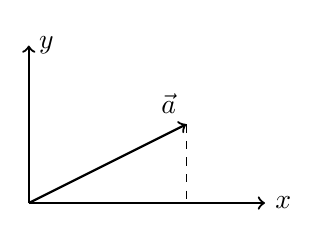
\begin{tikzpicture}
	\draw[thick, ->] (0,0)--(3,0) node[right] {$x$};
	\draw[thick, ->] (0,0)--(0,2) node[right] {$y$};
	\draw[thick, ->] (0,0)--(2,1) node[anchor = south east] {$\vec{a}$};
	\draw[dashed] (2,1)--(2,0);
	\end{tikzpicture}
\end{figure}

\prp{2.15.2. Властивості}\\
1) $\ker P = L_2$ \hspace{1cm} $\Im P = L_1$\\
2) $P^2 = P$\\
3) $L = \Im P  \oplus  \ker P$\\
\proof
1) $\forall z \in \ker P \iff Pz = x = 0 \iff z = y \in L_2$
$\forall w \in \Im P \iff w = Pz = x \in L_1$
\bigskip \\
2) $P^2z = P(Pz) = Px = P(x+0)=x=Pz$
\bigskip \\
3) \textit{випливає з означення} \qed
\bigskip \\
\prp{2.15.3.} Задано $P: L \to L$ - такий оператор, що $P^2 = P$\\
Тоді $P$ - оператор проєктування\\
\proof
1) Покажемо, що $\Im P \cap \ker P = \{0\}$\\
Дійсно, $\forall z \in (\Im P \cap \ker P) \Rightarrow \begin{cases} z \in \Im P \\ z \in \ker P \end{cases} \Rightarrow \begin{cases} z = Pw \\ Pz = 0 \end{cases}$\\
$\Rightarrow 0 = Pz = P^2z = P(Pz) = Pw = z$
\bigskip \\
2) Доведемо, що $L = \Im P  \oplus  \ker P$\\
Зафіксуємо елемент $w = z - Pz$, $z \in L$\\
Тоді $Pw = Pz - P(Pz) = Pz - P^2z = Pz - Pz = 0 \Rightarrow w \in \ker P$\\
$\Rightarrow z = \underset{\in \Im P}{Pz} + \underset{\in \ker P}{w}$\\
Отже, $\forall z \in L: \exists! x \in \Im P = L_1, \exists! y \in \ker P = L_2: z = x+y$\\
Оскільки $x \in \Im P$, то $x = Pw$\\
$\Rightarrow Pz = P(Pw+y) = P^2 w = Pw = x$\\
Остаточно, $P$ - оператор проєктування \qed
\bigskip \\
\rm{2.15.3.} Задано $P: L \to L$ - оператор проєктування, $L = \underset{=L_1}{\ker P}  \oplus  \underset{=L_2}{\Im P}$\\
$L_1,L_2$ - інваріантні підпростори (це вже було). Тоді $P = P|_{L_1}  \oplus  P|_{L_2}$\\
Дізнаємось, хто ці $P|_{L_1}, P|_{L_2}$\\
$z \in L_1 \Rightarrow z = x = x+0 \Rightarrow P|_{L_1}z = Pz = x = z$\\
Тобто $P|_{L_1} = I$ - тотожній оператор\\
$z \in L_2 \Rightarrow z = y \in \ker P \Rightarrow P|_{L_2} = Pz = Py = 0$\\
Тобто $P|_{L_2} = O$ - нульовий оператор\\
Тобто $P = I  \oplus  O$
\bigskip \\
Тепер покажемо, що є матрицею для оператора $P$\\
Нехай $\{e_1,\dots,e_k\}$ - базис $\Im P$ та $\{e_{k+1},\dots,e_n\}$ - базис $\ker P$\\
$Pe_1 = e_1 \dots Pe_k = e_k$\\
$Pe_{k+1} = 0 \dots Pe_n = 0$\\
Отже, маємо таку матрицю:\\
$\mathbb{P} = \begin{pmatrix}
1 & \dots & 0 & \vline & 0 & \dots & 0 \\
\vdots & \ddots & \vdots & \vline & \vdots & \ddots & \vdots \\
0 & \dots & 1 & \vline & 0 & \dots & 0 \\
\hline
0 & \dots & 0 & \vline & 0 & \dots & 0 \\
\vdots & \ddots & \vdots & \vline & \vdots & \ddots & \vdots \\
0 & \dots & 0 & \vline & 0 & \dots & 0 \\
\end{pmatrix} = \begin{pmatrix}
\mathbb{I}  & \vline & \mathbb{O} \\
 \hline
\mathbb{O} & \vline & \mathbb{O}
\end{pmatrix}$
\fi

\newpage
%\fi
% Дії з лінійними просторами (2)

% Нова ера з матрицями
%\iffalse
\setcounter{section}{3}
\setcounter{subsection}{0}
\section{Нова ера з матрицями}
\subsection{Власні числа та власні вектори}
\begin{definition}
Нехай $A \in \mathcal{L}(L)$.\\
\textbf{Власним вектором} оператора $A$ називається такий ненульовий елемент $f \in L$, для якого
\begin{align*}
\exists \lambda \in \mathbb{R}: Af = \lambda f.
\end{align*}
Водночас $\lambda$ називається \textbf{власним числом}\footnote{Англійською відповідно називаються eigenvector та eingenvalue (слово ''eigen'' взялось з німецької мови та переклдається як ''власний'').} оператора $A$.
\end{definition}

\begin{remark}
Із означення випливає, що власному вектору відповідає \emph{єдине} власне число в силу лінійності оператора. А власному числу може відповідати безліч власних векторів (\textit{див.\ нижче }\prpref{eigenspace_is_subspace})
\end{remark}

\begin{example}
Нехай оператор $A \colon \mathbb{R}^3 \to \mathbb{R}^3$ задається формулою:
\[
A \vec{x} = [\vec{x},\vec{a}].
\]
Тут записаний векторний добуток та $\vec{a} \in \mathbb{R}^3$ --- фіксований. Знайдемо власні числа та власні вектори оператора $A$.
\bigskip \\
Шукаємо такий вектор $\vec{f}$, щоб виконувалась рівність
\[
A \vec{f} = \lambda \vec{f} \implies [\vec{f},\vec{a}] = \lambda \vec{f}.
\]
Вектор $[\vec{f},\vec{a}]$ перпендикулярний до $\vec{f}$, але водночас дорівнює цьому вектору, який домножений на скаляр $\lambda$. Тож рівність виконується лише при $\lambda = 0$ --- знайшли власне число.\\
Числу $\lambda = 0$  відповідають власні вектори $A\vec{f} = \vec{0} \vec{f} = \vec{0}$, тобто $[\vec{f},\vec{a}] = \vec{0}$. Дана рівність означає, що $\vec{f} \parallel \vec{a}$. Отже, власними векторами будуть всі вектори, що паралельні $\vec{a}$.
\end{example}
\noindent
Зараз опишемо універсальний спосіб, як шукати власні вектори та власні числа.

\begin{corollary}
Справедливе наступне:
\begin{center}
$f$ --- власний вектор, якому відповідає власне число $\lambda \iff f \in \ker (A-\lambda I)$.
\end{center}
(\textit{випливає з означення власного вектора}).
\end{corollary}

\begin{proposition}
Нехай $A \in \mathcal{L}(L)$, якому відповідає матриця $\mathbb{A}$. Тоді
\begin{center}
$\lambda$ --- власне число оператора $A \iff \det(\mathbb{A} - \lambda \mathbb{I}) = 0$.
\end{center}
\end{proposition}

\begin{remark}
Дуже важливе питання має стояти, відносно якого базису записувати матрицю оператора. Насправді, різниці нема, нижче буде відповідне твердження.
\end{remark}

\begin{proof}
\rightproof Дано: $\lambda$ --- власне число $A$. Тоді існує ненульовий вектор $f \in \ker (A-\lambda I)$, тобто $\ker (A-\lambda I) \neq \{0\}$,  значить оператор $(A-\lambda I)$ не буде оборотним, а тому його матриця $\mathbb{A} - \lambda \mathbb{I}$ вироджена, тобто $\det (\mathbb{A} - \lambda \mathbb{I}) = 0$.
\bigskip \\
\leftproof Дано: $\det(\mathbb{A} - \lambda \mathbb{I}) = 0$, тобто оператор $A-\lambda I$ не оборотний, тому існує ненульовий вектор $f \in \ker (A-\lambda I)$, значить $f$ --- власний вектор та $\lambda$ --- власне число.
\end{proof}

\begin{proposition}
\label{change_of_basis_characteristic_polynomial}
Нехай $A \in \mathcal{L}(L)$, якому відповідають матриці $\mathbb{A}_f, \mathbb{A}_g$ в різних базисах $L$. Тоді
\begin{align*}
\det(\mathbb{A}_f - \lambda \mathbb{I}) = \det(\mathbb{A}_g - \lambda \mathbb{I}).
\end{align*}
\iffalse
Тобто неважливо, який там базис в просторі $L$, характеристичний многочлен той самий.
\fi
\end{proposition}

\begin{proof}
Матриці $\mathbb{A}_f, \mathbb{A}_g$ пов'язані тотожністю та діаграмою:
\begin{center}
\begin{tikzcd}
\mathbb{R}^n_f \arrow{rrr}{\mathbb{A}_{f}} \arrow{dd}[swap]{\mathbb{U}_{f \to g}} & & & \mathbb{R}^n_f \arrow{dd}{\mathbb{U}_{f \to g}} \\
& \arrow{lu}[swap]{J_f} L \arrow{r}{A} \arrow{ld}{J_g} & L \arrow{ru}{J_f} \arrow{rd}[swap]{J_g} \\
\mathbb{R}^n_g \arrow{rrr}{\mathbb{A}_{g}} & & & \mathbb{R}^n_g
\end{tikzcd}
\end{center}
\begin{align*}
\mathbb{A}_f = \mathbb{U}^{-1}_{f \to g} \mathbb{A}_g \mathbb{U}_{f \to g}.
\end{align*}
Нам відомо, що $\mathbb{U}_{f \to g}$ буде завжди невиродженою, тому дозволений такий ланцюг рівностей:
\begin{align*}
\det(\mathbb{A}_f - \lambda \mathbb{I}) = \det(\mathbb{U}^{-1}_{f \to g} \mathbb{A}_g \mathbb{U}_{f \to g} - \lambda \mathbb{I}) = \det(\mathbb{U}^{-1}_{f \to g} \mathbb{A}_g \mathbb{U}_{f \to g} - \lambda \mathbb{U}^{-1}_{f \to g} \mathbb{U}_{f \to g}) \\ = \det(\mathbb{U}^{-1}_{f \to g}(\mathbb{A}_g-\lambda \mathbb{I})\mathbb{U}_{f \to g}) = \det \mathbb{U}_{f \to g} \det \mathbb{U}_{f \to g}^{-1} \det (\mathbb{A}_g - \lambda \mathbb{I}) = \det (\mathbb{A}_g - \lambda \mathbb{I}).
\end{align*}
Отже, довели інваріантність відносно вибору базису.
\end{proof}

% don't need this
\iffalse
\begin{proposition}[Додаткові властивості власних чисел та векторів]
Нехай $A \in \mathcal{L}(L)$. Тоді:
\begin{enumerate}[nosep, wide=0pt, label={\arabic*)}]
\item $f$ --- власний вектор оператора $A$ з власним числом $\lambda \iff$ $f$ -- власний вектор оператора $(A - \mu I)$ з власним числом $(\lambda - \mu)$;
\item Якщо $\{g_1,\dots,g_n\}$ --- базис $L$ та $\mathbb{A}_g$ --- матриця $A$ для нашого базису, то $\lambda$ --- власне число $A$ $\iff$ $\lambda$ --- власне число $\mathbb{A}_g$ та $f$ -- власний вектор $A$ з власним числом $\lambda$ $\iff$ $J_g f$ --- власний вектор $\mathbb{A}_g$.
\end{enumerate}
\end{proposition}

\begin{proof}
\begin{enumerate}[topsep =0pt, wide=0pt, label={\arabic*)},topsep=-\parskip]
\item $f$ -- власний вектор $A$ з власним числом $\lambda \iff Af = \lambda f \iff Af - \mu f = \lambda f - \mu f \iff \\ \iff Af - \mu If = (\lambda - \mu)f \iff (A-\mu I)f = (\lambda - \mu)f \iff$ $f$ -- власний вектор $(A- \mu I)$ з власним число $(\lambda - \mu)$.

\item Маємо наступну картину:\\
\begin{tikzcd}
L \arrow{r}{A} \arrow{d}[swap]{J_g} & L \arrow{d}{J_g} \\
\mathbb{R}^n \arrow{r}{\mathbb{A}_g} & \mathbb{R}^n
\end{tikzcd}\\
Тоді $Af = J_g^{-1} \mathbb{A}_g J_g f = \lambda f$. Обидві частини множимо на $J_g \implies \mathbb{A}_g (J_g f) = \lambda (J_g f)$. \qedhere
\end{enumerate}
\end{proof}
\fi

\begin{definition}
Нехай $A \in \mathcal{L}(L)$, в якому $\lambda$ --- власне число.\\
\textbf{Власним підпростором}\footnote{Англійською такий підпростір називають eigenspace.} оператора $A$ називають множину всіх власних векторів з відповідним власним числом $\lambda$ та нульвоим вектором.\\
\textit{Позначення}: $L_{\lambda}$.
\end{definition}

\begin{corollary}
\label{eigenspace_is_subspace}
$L_\lambda = \ker(A-\lambda I)$.\\
(\textit{таким чином, $L_{\lambda}$ --- автоматично інваріантний підпростір лінійного простору $L$.})
\end{corollary}

\begin{remark}
Далі якщо розглянути $A|_{L_{\lambda}}$, то він матиме лише єдине власне число $\lambda$ (\textit{бо кожному власному вектору з $L_{\lambda}$ ставиться єдине лише власне число $\lambda$}).
\end{remark}

\begin{proposition}
Нехай $A \in \mathcal{L}(L)$ та $f_1,\dots,f_k$ --- власні вектори з попарно різними власними числами. Тоді $\{f_1,\dots,f_k\}$ --- л.н.з.
\end{proposition}

\begin{proof}
Доведення проведемо за МІ по кількості власних векторів.
\begin{enumerate}[nosep,wide=0pt,label={\Roman*.}]
\item \textit{База індукції}. При $k=1$ маємо $\{f_1\}$ --- л.н.з. автоматично.
\item \textit{Припущення індукції}. Нехай $\{f_1,\dots,f_k\}$ --- л.н.з. для деякого $k$.
\item \textit{Крок індукції}. Доведемо, що система $\{f_1,\dots,f_k, f_{k+1}\}$ --- л.н.з. Нехай
\[
\alpha_1 f_1 + \dots + \alpha_k f_k + \alpha_{k+1} f_{k+1} = 0.
\]
Подіємо оператором $A$ на обидві частини рівності. Ліва частина буде такою:
\begin{align*}
A(\alpha_1 f_1 + \dots + \alpha_k f_k + \alpha_{k+1} f_{k+1}) & = \alpha_1 Af_1 + \dots + \alpha_k Af_k + \alpha_{k+1} Af_{k+1} \\
& = \alpha_1 \lambda_1 f_1 + \dots + \alpha_k \lambda_k f_k + \alpha_{k+1} \lambda_{k+1} f_{k+1}.
\end{align*}
Разом одержимо рівняння
\[
\alpha_1 \lambda_1 f_1 + \dots + \alpha_k \lambda_k f_k + \alpha_{k+1} \lambda_{k+1} f_{k+1} = 0.
\]
Із найпершого рівняння можна виразити $\alpha_{k+1} f_{k+1}$, тоді
\[
\alpha_{k+1}f_{k+1} = -\alpha_1 f_1 - \dots - \alpha_k f_k.
\]
Його підставимо в рівняння, яке отримала після дії оператором --- отримаємо:
\[
\alpha_1 (\lambda_1 - \lambda_{k+1})f_1 + \dots + \alpha_k (\lambda_k - \lambda_{k+1})f_k = 0 \overset{\textrm{л.н.з.}}{\implies} \alpha_1(\lambda_1 - \lambda_{k+1})=0, \dots, \alpha_k(\lambda_k - \lambda_{k+1}) = 0.
\]
Оскільки власні числа попарно різні, то звідси $\alpha_1 = \dots = \alpha_k = 0$. Отримані значення підставимо в найперше рівняння. Там отримаємо $\alpha_{k+1} = 0$.\\
Остаточно, $\{f_1,\dots,f_k, f_{k+1}\}$ --- л.н.з.
\end{enumerate}
МІ доведено.
\end{proof}

\subsection{Характеристичний многочлен}
\begin{definition}
Нехай $A \in \mathcal{L}(L)$. \\
\textbf{Характеристичним многочленом} називається вираз
\begin{align*}
\chi(\lambda) = \det(A - \lambda I)\footnotemark.
\end{align*}
Саме рівняння називається \textbf{характеристичним рівнянням}\footnote{Я тепер пишу всередині визначника оператор $A - \lambda I$, оскільки нема різниці, відносно якого базису будувати матрицю.} .
\end{definition}

Ми нарешті побудували алгоритм, як шукати власне число, а згодом власний вектор.

\begin{example}
\label{find_eigenvectors}
Знайдемо всі власні числа та власні вектори матриці
\[
\mathbb{A} = \begin{pmatrix}
4 & -1 & -2 \\
2 & 1 & -2 \\
1 & -1 & 1
\end{pmatrix}.
\]
\begin{enumerate}[wide=0pt,label={\Roman*.}]
\item \textit{Пошук власних чисел}. \\
Дана процедура проводиться через характеристичне рівняння
\[
\det (\mathbb{A} - \lambda \mathbb{I}) = 0.
\]
Розпишемо цей многочлен детальніше:
\begin{multline*}
\det (\mathbb{A} - \lambda \mathbb{I}) = \det \begin{pmatrix}
4-\lambda & -1 & -2 \\
2 & 1-\lambda & -2 \\
1 & -1 & 1-\lambda
\end{pmatrix} \\
= (4-\lambda)(1-\lambda)(1-\lambda) + 2 + 2 + 2(1-\lambda) -2(4-\lambda) +2(1-\lambda) = -\lambda^3 + 6 \lambda^2 - 11 \lambda + 6.
\end{multline*}
Разом отримали кубічне рівняння, яке можна самостійно добити:
\[
-\lambda^3 + 6 \lambda^2 - 11 \lambda + 6 = 0 \implies (\lambda - 1)(\lambda -2)(\lambda - 3) = 0.
\]
Отже, $\{1,2,3\}$ задає множину всіх власних чисел оператора $A$.

\item \textit{Пошук власних векторів}.\\
Треба пройтись по кожному власному числу. Власних векторів буде багато, тому тут радше ми шукаємо власний підпростір.
\begin{itemize}[wide=0pt]
\item $\lambda_1 = 1$.
Тоді маємо наступне:
\[
(\mathbb{A} - \lambda_1 \mathbb{I})\vec{f} =\begin{pmatrix}
3 & -1 & -2 \\
2 & 0 & -2 \\
1 & -1 & 0
\end{pmatrix} \vec{f} = \vec{0} \implies \begin{cases} 2f_1 - 2f_3 = 0; \\ f_1 - f_2 = 0. \end{cases} \implies f_1 = f_2 = f_3. 
\]
Таким чином, власний підпростір матиме вигляд: 
\[
L_{\lambda_1} = \linspan\left\{ \begin{pmatrix}
1 \\ 1 \\ 1
\end{pmatrix} \right\}.
\]

\item $\lambda_2 = 2$
Тоді маємо наступне:
\[
(\mathbb{A} - \lambda_2 \mathbb{I})\vec{f} =\begin{pmatrix}
2 & -1 & -2 \\
2 & -1 & -2 \\
1 & -1 & -1
\end{pmatrix} \vec{f} = \vec{0} \implies \begin{cases} 2f_1 - f_2 - 2f_3 = 0; \\ f_1 - f_2 - f_3 = 0. \end{cases} \implies \begin{cases} f_1 = f_3 \\ f_2 = 0. \end{cases}
\]
Таким чином, власний підпростір матиме вигляд: 
\[
L_{\lambda_2} = \linspan\left\{ \begin{pmatrix}
1 \\ 0 \\ 1
\end{pmatrix} \right\}.
\]

\item $\lambda_3 = 3$.
Тоді маємо наступне:
\[
(\mathbb{A} - \lambda_3 \mathbb{I})\vec{f} =\begin{pmatrix}
1 & -1 & -2 \\
2 & -2 & -2 \\
1 & -1 & -2
\end{pmatrix} \vec{f} = \vec{0} \implies \begin{cases} 2f_1 - 2f_2 - 2f_3 = 0; \\ f_1 - f_2 - 2f_3 = 0. \end{cases} \implies \begin{cases} f_1 = f_2 \\ f_3 = 0. \end{cases}
\]
Таким чином, власний підпростір матиме вигляд:
\[
L_{\lambda_3} = \linspan\left\{ \begin{pmatrix}
1 \\ 1 \\ 0
\end{pmatrix} \right\}.
\]
\end{itemize}
\end{enumerate}
\end{example}

\begin{example}
Знайти власні числа оператора $A \colon \mathbb{R}_2[x] \to \mathbb{R}_2[x]$, що задається як
\[
A(ax^2+bx+c) = bx^2 + cx.
\]
Нам потрібна матриця оператора, для цього оберемо базис. Ми довели, що характеристичний многочлен від базиса не залежить, тож оберемо зручний $\{1,x,x^2\}$. Тоді
\[
\begin{gathered} A1 = 0 \cdot 1 + 1 \cdot x + 0 \cdot x^2; \\ Ax = 0 \cdot 1 + 0 \cdot x + 1 \cdot x^2; \\ Ax^2 = 0 \cdot 1 + 0 \cdot x + 0 \cdot x^2. \end{gathered} \implies \mathbb{A} = \begin{pmatrix}
0 & 0 & 0 \\
1 & 0 & 0 \\
0 & 1 & 0
\end{pmatrix}.
\]
Тож $\det (\mathbb{A}-\lambda \mathbb{I}) = -\lambda^3$, а тому $\lambda = 0$ --- єдине власне число.
\end{example}

\begin{theorem}
Характеристичний многочлен має таку формулу:
\begin{align*}
\chi(\lambda) = \displaystyle (-1)^n \lambda^n + (-1)^{n-1} \tr \mathbb{A} \cdot \lambda^{n-1} + \sum_{k=2}^{n-1} \left( \sum_{1 \leq j_1 < j_2 < \dots < j_k \leq n} (-1)^{n-k} M_{j_1 \dots j_k}^{j_1 \dots j_k} \right) \lambda^{n-k} + \det \mathbb{A}.
\end{align*}
\textit{Словесно опишу многочлен: вільний коефіцієнт --- це $\det \mathbb{A}$; коефіцієнт при $\lambda$ --- це сума всіх можливих мінорів порядка $n-1$; коефіцієнт при $\lambda^2$ --- це сума всіх можливих мінорів порядка $n-2$ тощо. Кожний одночлен чередується знаком, починаючи з вільного коефіцієнта.}
\end{theorem}

\begin{remark}
Розглянемо випадок матриці $\mathbb{A}$ розмірності $2 \times 2$ для розуміння.
\[
\det (\mathbb{A} - \lambda \mathbb{I}) = \det \begin{pmatrix}
a_{11}-\lambda & a_{12} \\
a_{21} & a_{22} - \lambda
\end{pmatrix} = \lambda^2 - (a_{11}+a_{22})\lambda + \det \mathbb{A}.
\]

Далі розглянемо матрицю $\mathbb{A}$ розмірності $3 \times 3$, аналогічно для повного розуміння.
\begin{align*}
\det (\mathbb{A} - \lambda \mathbb{I}) = \det \begin{pmatrix}
a_{11}-\lambda & a_{12} & a_{13} \\
a_{21} & a_{22}-\lambda & a_{23} \\
a_{31} & a_{32} & a_{33}-\lambda \\
\end{pmatrix} = -\lambda^3 + (a_{11}+a_{22}+a_{33})\lambda^2 - \\ - \left(\underset{=M_{12}^{12}}{\det \begin{pmatrix}
a_{11} & a_{12} \\
a_{21} & a_{22}
\end{pmatrix}} - \underset{=M_{13}^{13}}{\det \begin{pmatrix}
a_{11} & a_{13} \\
a_{31} & a_{33}
\end{pmatrix}} + \underset{=M_{23}^{23}}{\det \begin{pmatrix}
a_{22} & a_{23} \\
a_{32} & a_{33}
\end{pmatrix}} \right)\lambda + \det \mathbb{A}.
\end{align*}
Зауважимо, що коефіцієнт при $\lambda$ є сумою головних мінорів (\textit{тобто тих мінорів, де номера рядка та стовпчиків співпадають}).
\end{remark}

\begin{proof}
Тепер розглянемо матрицю $\mathbb{A}$ загальної розмірності $n \times n$.
\[
\det (\mathbb{A} - \lambda \mathbb{I}) = \det \begin{pmatrix}
a_{11}-\lambda & a_{12} & \dots & a_{1n} \\
a_{21} & a_{22} - \lambda & \dots & a_{2n} \\
\vdots & \vdots & \ddots & \vdots \\
a_{n1} & a_{n2} & \dots & a_{nn}-\lambda
\end{pmatrix}.
\]
Аналізуємо цю матрицю:
\begin{itemize}[nosep,wide=0pt]
\item доданок при $\lambda^n$ отримується при множенні тільки елементів головної діагоналі, тобто маємо коефіцієнт $(-1)^n$:
\[
\begin{pmatrix}
a_{11}-\textcolor{red}{\lambda} & a_{12} & \dots & a_{1n} \\
a_{21} & a_{22}-\textcolor{red}{\lambda} & \dots & a_{2n} \\
\vdots & \vdots & \ddots & \vdots \\
a_{n1} & a_{n2} & \dots & a_{nn}-\textcolor{red}{\lambda}
\end{pmatrix}.
\]
\item доданок при $\lambda^{n-1}$ отримується при множенні всіх елементів головної діагоналі, крім, можливо, одного, по черзі, тобто маємо коефіцієнти: 
\[
(-1)^{n-1}a_{11} + (-1)^{n-1}a_{22} + \dots + (-1)^{n-1}a_{nn} = (-1)^{n-1}(a_{11}+a_{22}+\dots+a_{nn}).
\]
Схематично це ось так:
\begin{align*}
\begin{pmatrix}
\textcolor{red}{a_{11}}-\lambda & a_{12} & \dots & a_{1n} \\
a_{21} & a_{22}-\textcolor{red}{\lambda} & \dots & a_{2n} \\
\vdots & \vdots & \ddots & \vdots \\
a_{n1} & a_{n2} & \dots & a_{nn}-\textcolor{red}{\lambda}
\end{pmatrix},\ \begin{pmatrix}
a_{11}-\textcolor{red}{\lambda} & a_{12} & \dots & a_{1n} \\
a_{21} & \textcolor{red}{a_{22}}-\lambda & \dots & a_{2n} \\
\vdots & \vdots & \ddots & \vdots \\
a_{n1} & a_{n2} & \dots & a_{nn}-\textcolor{red}{\lambda}
\end{pmatrix},\ \dots,\\
\begin{pmatrix}
a_{11}-\textcolor{red}{\lambda} & a_{12} & \dots & a_{1n} \\
a_{21} & a_{22}-\textcolor{red}{\lambda} & \dots & a_{2n} \\
\vdots & \vdots & \ddots & \vdots \\
a_{n1} & a_{n2} & \dots & \textcolor{red}{a_{nn}}-\lambda
\end{pmatrix}.
\end{align*}
\item доданок при $\lambda^{n-2}$ отримується при множенні всіх елементів головної діагоналі, крім, можливо, двох, по черзі. Наприклад, розглянемо один із доданків, в якому множимо елементи головної діагоналі з номерами $3,4,\dots,n$, при множенні цих елементів обираємо $\lambda^{n-2}$, залишається цей вираз помножити на
\[
\det \begin{pmatrix}
a_{11}-\lambda & a_{12} \\
a_{21} & a_{22}-\lambda
\end{pmatrix} = \lambda^2 - (a_{11}+a_{22})\lambda + \det \begin{pmatrix}
a_{11} & a_{12} \\
a_{21} & a_{22}
\end{pmatrix}.
\]
Оскільки нам потрібний степінь $n-2$, то ми обираємо останній доданок, що є $M_{12}^{12}$.\\
Для інших випадків все аналогічно. Загалом маємо коефіцієнт при $\lambda^{n-2}:$
\[
(-1)^{n-2} (M_{12}^{12} + M_{13}^{13} + \dots + M_{1n}^{1n} + M_{23}^{23} + \dots + M_{2n}^{2n} + \dots + M_{n-1,n}^{n-1,n} + M_{nn}^{nn}) = (-1)^{n-2} \displaystyle \sum_{1 \leq j < m \leq n} M_{jm}^{jm}.
\]
У кінці отримали суму всіх головних мінорів 2-го порядку. Схематично все це робиться так:
\begin{align*}
\begin{pmatrix}
\textcolor{red}{a_{11}}-\lambda & \textcolor{red}{a_{12}} & a_{13} & \dots & a_{1n} \\
\textcolor{red}{a_{21}} & \textcolor{red}{a_{22}}-\lambda & a_{23} & \dots & a_{2n} \\
a_{31} & a_{32} & a_{33}-\textcolor{red}{\lambda} & \dots & a_{3n} \\
\vdots & \vdots & \vdots & \ddots & \vdots \\
a_{n1} & a_{n2} & a_{n3} & \dots & a_{nn}-\textcolor{red}{\lambda}
\end{pmatrix} ,\
\begin{pmatrix}
\textcolor{red}{a_{11}}-\lambda & a_{12} & \textcolor{red}{a_{13}} & \dots & a_{1n} \\
a_{21} & a_{22} - \textcolor{red}{\lambda} & a_{23} & \dots & a_{2n} \\
\textcolor{red}{a_{31}} & a_{32} & \textcolor{red}{a_{33}}-\lambda & \dots & a_{3n} \\
\vdots & \vdots & \vdots & \ddots & \vdots \\
a_{n1} & a_{n2} & a_{n3} & \dots & a_{nn}-\textcolor{red}{\lambda}
\end{pmatrix} ,\
\dots, \\
\begin{pmatrix}
\textcolor{red}{a_{11}}-\lambda & a_{12} & a_{13} & \dots & \textcolor{red}{a_{1n}} \\
a_{21} & a_{22} - \textcolor{red}{\lambda} & a_{23} & \dots & a_{2n} \\
a_{31} & a_{32} & a_{33}-\textcolor{red}{\lambda} & \dots & a_{3n} \\
\vdots & \vdots & \vdots & \ddots & \vdots \\
\textcolor{red}{a_{n1}} & a_{n2} & a_{n3} & \dots & \textcolor{red}{a_{nn}}-\lambda
\end{pmatrix},\ \begin{pmatrix}
a_{11} - \textcolor{red}{\lambda} & a_{12} & a_{13} & \dots & a_{1n} \\
a_{21} & \textcolor{red}{a_{22}} - \lambda & \textcolor{red}{a_{23}} & \dots & a_{2n} \\
a_{31} & \textcolor{red}{a_{32}} & \textcolor{red}{a_{33}}-\lambda & \dots & a_{3n} \\
\vdots & \vdots & \vdots & \ddots & \vdots \\
a_{n1} & a_{n2} & a_{n3} & \dots & a_{nn}-\textcolor{red}{\lambda}
\end{pmatrix},\
\dots,
\end{align*}

\begin{align*}
\begin{pmatrix}
a_{11} - \textcolor{red}{\lambda} & a_{12} & a_{13} & \dots & a_{1n} \\
a_{21} & \textcolor{red}{a_{22}} - \lambda & a_{23} & \dots & \textcolor{red}{a_{2n}} \\
a_{31} & a_{32} & a_{33} - \textcolor{red}{\lambda} & \dots & a_{3n} \\
\vdots & \vdots & \vdots & \ddots & \vdots \\
a_{n1} & \textcolor{red}{a_{n2}} & a_{n3} & \dots & \textcolor{red}{a_{nn}}-\lambda
\end{pmatrix},\ \dots ,\ \dots, \begin{pmatrix}
a_{11}-\textcolor{red}{\lambda} & a_{12} & \dots & a_{1n} \\
a_{21} & a_{22} - \textcolor{red}{\lambda} & \dots & a_{2n} \\
\vdots & \vdots & \textcolor{red}{\ddots} & \textcolor{red}{\vdots} \\
a_{n1} & a_{n2} & \textcolor{red}{\dots} & \textcolor{red}{a_{nn}}-\lambda
\end{pmatrix}.
\end{align*}
\item все аналогічно для $\lambda^{n-3}$, коефіцієнтом буде
\[
(-1)^{n-3} \displaystyle \sum_{1 \leq j < m < p \leq n} M_{jmp}^{jmp},
\]
де тут зібралась сума всіх головних мінорів 3-го порядку.\\
\vdots
\item нарешті, коефіцієнтом вільного доданку буде якраз $\det \mathbb{A}$.
\[
\begin{pmatrix}
\textcolor{red}{a_{11}}-\lambda & \textcolor{red}{a_{12}} & \textcolor{red}{\dots} & \textcolor{red}{a_{1n}} \\
\textcolor{red}{a_{21}} & \textcolor{red}{a_{22}} - \lambda & \textcolor{red}{\dots} & \textcolor{red}{a_{2n}} \\
\textcolor{red}{\vdots} & \textcolor{red}{\vdots} & \textcolor{red}{\ddots} & \textcolor{red}{\vdots} \\
\textcolor{red}{a_{n1}} & \textcolor{red}{a_{n2}} & \textcolor{red}{\dots} & \textcolor{red}{a_{nn}}-\lambda
\end{pmatrix}.
\]
\end{itemize}
Збираючи все в кучку, отримаємо наступне:
\begin{multline*}
\det (\mathbb{A} - \lambda \mathbb{I}) = \displaystyle (-1)^n \lambda^n + (-1)^{n-1} (a_{11} + a_{22} + \dots + a_{nn}) \lambda^{n-1} + (-1)^{n-2} \sum_{1 \leq j < m \leq n} M_{jm}^{jm} \lambda^{n-2} \\ + (-1)^{n-3} \sum_{1 \leq j < m < p \leq n} M_{jmp}^{jmp} \lambda^{n-3} + \dots + \det \mathbb{A} \\
= (-1)^n \lambda^n + \sum_{k=1}^{n-1} (-1)^{n-k} \left( \sum_{1 \leq j_1 < j_2 < \dots < j_k} M_{j_1j_2\dots j_k}^{j_1j_2\dots j_k} \lambda^{n-k} \right) + \det \mathbb{A}. \qedhere
\end{multline*}
\end{proof}

\begin{corollary}
Існує інший способ, як обчислити слід матриці:
\begin{align*}
\tr \mathbb{A} = \displaystyle\sum_{i=1}^n \lambda_i.
\end{align*}
(\textit{за умовою, що $\chi(\lambda)$ розкладається на лінійні множники, на множині $\mathbb{C}$ це завжди можна}).
\end{corollary}

\begin{proof}
Дійсно, уже з'ясували, що коефцієнтом многочлена $\chi(\lambda)$ при $\lambda^{n-1}$ буде якраз $\tr \mathbb{A}$. За умовою, що допускаємо розклад $\chi(\lambda)$ на лінійні множники, тобто
\[
\chi(\lambda) = (\lambda-\lambda_1) \dots (\lambda - \lambda_n),
\]
то, прирівнюючи коефіцієнти многочленів, одержимо бажану формулу.
\end{proof}

\begin{example}
За щойно доведеною формулою знайдемо характеристичний многочлен для той самої матриці 
\[
\mathbb{A} = \begin{pmatrix}
4 & -1 & -2 \\
2 & 1 & -2 \\
1 & -1 & 1
\end{pmatrix}.
\]
Маємо ось таке:
\begin{align*}
\det (\mathbb{A} - \lambda \mathbb{I}) = -\lambda^3 + (4+1+1)\lambda^2 - \left( \begin{vmatrix}
4 & -1 \\
2 & 1
\end{vmatrix} + \begin{vmatrix}
4 & -2 \\
1 & 1
\end{vmatrix} + \begin{vmatrix}
1 & -2 \\
-1 & 1
\end{vmatrix} \right) \lambda + \begin{vmatrix}
4 & -1 & -2 \\
2 & 1 & -2 \\
1 & -1 & 1
\end{vmatrix} \\
=-\lambda^3 + 6\lambda^2 - (6+6-1)\lambda + (4+2+4+2-8+2) = -\lambda^3 + 6\lambda^2 -11\lambda + 6.
\end{align*}
\end{example}

\subsection{Діагоналізація матриці, алгебраїчне та геометричне кратне}
\begin{definition}
Нехай $A \in \mathcal{L}(L,L)$. \\
Оператор $A$ називають \textbf{діагоналізовним}, якщо існує базис, відносно якого матриця оператора базисі є діагоналізовною, тобто
\begin{align*}
\mathbb{A} = \begin{pmatrix}
a_{11} & \dots & 0 \\
\vdots & \ddots & \vdots \\
0 & \dots & a_{nn}
\end{pmatrix}.
\end{align*}
\end{definition}

Перш ніж наводити якісь приклади, треба знайти інший способ зрозуміти, коли оператор буде діагоналізовним.

\begin{definition}
Нехай $A \in \mathcal{L}(L)$ та $\lambda_0$ --- власне число.\\
\textbf{Алгебраїчним кратним} назвемо кратність кореня $\lambda_0$ характеристичного многочлена.\\
\textbf{Геометричним кратним} назвемо розмірність власного підпростору, тобто $\dim L_{\lambda_0}$.\\
\textit{Відповідні позначення}: $a_{\lambda_0},\ g_{\lambda_0}$.
\end{definition}

\begin{lemma}
Нехай $A \in \mathcal{L}(L)$ та $M$ --- $A$-інваріантний підпростір. Тоді $\chi_{A|_M}(\lambda) \mid \chi_A(\lambda)$ (\textit{один характеристичний многочлен ділить інший}).
\end{lemma}

\begin{proof}
Оскільки $M$ --- інваріантний відносно $A$, то існує базис, де
\[
\mathbb{A} = \begin{pmatrix}
\mathbb{A}|_{M} & \vline & * \\
\hline
\mathbb{O} & \vline & \mathbb{A}_{L/_M}
\end{pmatrix}.
\]
Згадавши деякі властивості визначника, одержимо наступне:
\[
\det (\mathbb{A} - \lambda \mathbb{I}) = \det \begin{pmatrix}
\mathbb{A}|_{M}- \lambda \mathbb{I} & \vline & \mathbb{C} \\
\hline
\mathbb{O} & \vline & \mathbb{A}_{L/_M}- \lambda \mathbb{I}
\end{pmatrix} = \det(\mathbb{A}|_M-\lambda \mathbb{I}) \det (\mathbb{A}_{L/_M} - \lambda \mathbb{I}).
\]
Що й доводить твердження. Тобто $\chi_{A|_M}(\lambda) \mid \chi_A(\lambda)$.
\end{proof}

\begin{corollary}
Нехай $A \in \mathcal{L}(L)$ та $\lambda_0$ --- власне число. Тоді $a_{\lambda_0} \geq g_{\lambda_0}$.
\end{corollary}

\begin{proof}
Розглянемо простір $L_{\lambda_0}$, який інваріантний, позначимо $\dim L_{\lambda_0} = k$. Відомо, що $A|_{L_{\lambda_0}}$ має лише єдине власне число $\lambda_0$, тому $\chi_{A|_{\lambda_0}}(\lambda) = (\lambda-\lambda_0)^k$. Оскільки $\chi_{A|_{\lambda_0}} \mid \chi_A$, то маємо наступне:
\[
\chi_A(\lambda) = (\lambda-\lambda_0)^k \cdot p(\lambda).
\]
Тому кратність кореня $\lambda_0$ уж точно не менше за $k$. Тобто $a_{\lambda_0} \geq k = \dim L_{\lambda_0} = g_{\lambda_0}$.
\end{proof}

\begin{example}
Якщо побачити \exref{non_diagonalizable_because_not_enough_dim}, то там $a_{\lambda=-2} = 2$, але $g_{\lambda = -2} = 1$. Забігаючи наперед, саме через різну кратність ми не маємо діагоналізовності матриці.
\end{example}

\begin{proposition}
Нехай $A \in \mathcal{L}(L)$ та $\lambda_1,\dots,\lambda_k$ --- різні власні числа. Тоді власні підпростори $L_{\lambda_1},\dots, L_{\lambda_k}$ утворюють пряму суму.
\end{proposition}

\begin{proof}
Для прямої суми треба показати, що 
\[
L_{\lambda_i} \cap \left( L_{\lambda_1} + \underset{\text{без }i}{\dots} + L_{\lambda_k} \right) = \{0\}, \quad i = 1,\dots,k.
\]
Зрозуміло, що там нулевий елемент лежить. Не встрачаючи загальності, розглянемо випадок $i = 1$.\\
!Припустимо, що $x \in L_{\lambda_1} \cap (L_{\lambda_2} + \dots + L_{\lambda_k})$, який ненулевий. Оскільки $x \in L_{\lambda_1}$, то $x$ --- власний вектор для власного числа $\lambda_1$. Також 
\[
x = f_2 + \dots + f_k
\]
за означенням суми. Із цієї рівності випливає, що система $\{x,f_2,\dots,f_k\}$ --- л.з. система. Проте, оскільки $\lambda_1,\dots,\lambda_k$ --- різні, дана система має бути л.н.з. --- суперечність!
\end{proof}

\begin{theorem}[Критерій діагонізовності матриці]
Нехай $A \in \mathcal{L}(L)$. Задані умови еквівалентні:
\begin{enumerate}[nosep,wide=0pt,label={\arabic*)}]
\item $A$ --- діагоналізовний;
\item $\chi_A(\lambda) = \displaystyle\prod_{i=1}^k (\lambda_i - \lambda)^{\alpha_i}$, причому для кожного власного числа $\lambda_i$ маємо $a_{\lambda_i} = g_{\lambda_i}$;
\item $L = L_{\lambda_1} \oplus \dots \oplus L_{\lambda_k}$;
\item існує базис простору $L$ із суто власних векторів.
\end{enumerate}
\end{theorem}

\begin{proof}
$\boxed{1) \Rightarrow 2)}$ Дано: $A$ --- діагоналізовний, тобто
\[ 
\mathbb{A} = \begin{pmatrix}
\mu_1 & \dots & 0 \\
\vdots & \ddots & \vdots \\
0 & \dots & \mu_n
\end{pmatrix}.
\]
Звідси випливає, що 
\[
\chi_A(\lambda) = \det (\mathbb{A}-\lambda \mathbb{I}) = (\mu_1 - \lambda) \dots (\mu_n - \lambda).
\]
Але оскільки деякі $\mu_1,\dots,\mu_n$ можуть збігатися, то ми запишемо в такому вигляді:\\
\[
\chi_A(\lambda) = \displaystyle\prod_{i=1}^k (\lambda_i - \lambda)^{\alpha_i},
\]
де $\lambda_i \neq \lambda_j$ при $i \neq j$. Оскільки $\lambda_i$ --- власне число, то тоді $a_{\lambda_i} \geq g_{\lambda_i}$.\\
Даній матриці $\mathbb{A}$ відповідає базис $\{f_1,\dots,f_n\}$, серед векторів оберемо підсистему $\{f_{i_1},\dots,f_{i_{\alpha_i}}\}$, у яких власне число $\lambda_i$ (\textit{це також л.н.з. система}). Звідси $\linspan \{f_{i_1},\dots,f_{i_{\alpha_i}}\} \subset L_{\lambda_i}$, але тоді $g_{\lambda_i} = \dim L_{\lambda_i} \geq \alpha_i = a_i$.
\bigskip \\
$\boxed{2) \Rightarrow 3)}$ Дано: $\chi_A(\lambda) = \displaystyle\prod_{i=1}^k (\lambda_i - \lambda)^{\alpha_i}$, причому $a_{\lambda_i} = g_{\lambda_i}$. Тобто $\dim L_{\lambda_i} = a_{\lambda_i}$. По-перше, 
\[
a_{\lambda_1} + \dots + a_{\lambda_k} = \alpha_1 + \dots + \alpha_k = n,
\]
оскільки степінь многочлена буде $n$; по-друге, оскільки $L_{\lambda_1},\dots, L_{\lambda_k}$ утворюють пряму суму, то об'єднавши їхні базиси, отримаємо базис $L$, просто тому що кількість базисних елементів $n$ штук. Тоді за \thref{direct_sum_iff_union_of_bases_is_basis}, $L = L_{\lambda_1} \oplus \dots \oplus L_{\lambda_k}$.
\bigskip \\
$\boxed{3) \Rightarrow 4)}$ Дано: $L = L_{\lambda_1} \oplus \dots \oplus L_{\lambda_k}$. Нехай $\{h_1^i,\dots,h^i_{m_i}\}$ --- базис $L_{\lambda_i}$, тоді за \thref{direct_sum_iff_union_of_bases_is_basis}, буде базис $L$, який складається з $n$ елементів, кожний з яких --- власний вектор.
\bigskip \\
$\boxed{4) \Rightarrow 1)}$ Дано: $\{f_1,\dots,f_n\}$ --- базис власних векторів. Кожний з власних векторів має своє власне число. Побудуємо тоді матрицю оператора:
\begin{align*}
Af_1 = \lambda_1 f_1 = \lambda_1 f_1 + 0 f_2 + \dots + 0 f_n;\\
Af_2 = \lambda_2 f_2 = 0 f_1 + \lambda_2 f_2 + \dots + 0 f_n;\\
\vdots\\
Af_n = \lambda_n f_n = 0 f_1 + 0 f_2 + \dots + \lambda_n f_n.
\end{align*}
Тоді матриця оператора $A$ в базисі власних векторів має вигляд:
\[
\mathbb{A}_f = \begin{pmatrix}
\lambda_1 & 0 & \dots & 0 \\
0 & \lambda_2 & \dots & 0 \\
\vdots & \vdots & \ddots & \vdots \\
0 & 0 & \dots & \lambda_n
\end{pmatrix}.
\]
Отже, матрицю діагоналізували.
\end{proof}

\begin{example}
Повернимось до \exref{find_eigenvectors}. У оператора, що був заданий матрицею $\mathbb{A}$, ми знайшли 3 власних числа: $\lambda_1 = 1, \lambda_2 = 2,\lambda_3 = 3$. Також ми знайшли власні підпростори, від кожного з яких оберемо базисний власний вектор:
\begin{align*}
\vec{f}_1 = \begin{pmatrix}
1 \\ 1 \\ 1
\end{pmatrix},\ \vec{f}_2 = \begin{pmatrix}
1 \\ 0 \\ 1
\end{pmatrix},\ \vec{f}_3 = \begin{pmatrix}
1 \\ 1 \\ 0
\end{pmatrix}.
\end{align*}
Вектори $\{\vec{f}_1,\vec{f}_2,\vec{f}_3\}$ утворюють базис в $\mathbb{R}^3$. Тому наш оператор має діагоналізовану матрицю 
\[
\mathbb{D} = \begin{pmatrix}
1 & 0 & 0 \\
0 & 2 & 0 \\
0 & 0 & 3
\end{pmatrix}.
\]
Записали по порядку власні числа для кожного власного вектора.
\end{example}

\iffalse
Ба більше, ми можемо розкрити деякі цікаві факти\\
\begin{tikzcd}
\mathbb{R}^3_f \arrow{r}{\mathbb{A}_f} \arrow{d}[swap]{U} & \mathbb{R}^3_f \arrow{d}{U} \\
\mathbb{R}^3_e \arrow{r}{A} & \mathbb{R}^3_e
\end{tikzcd}\\
Тут $U = \begin{pmatrix}
1 & 1 & 1 \\
1 & 0 & 1 \\
1 & 1 & 0 \\
\end{pmatrix}$\\
З картинки можна знайти:\\
$A = U \mathbb{A}_f U^{-1}$\\
$A^2 = A\cdot A = U \mathbb{A}_f U^{-1} U \mathbb{A}_f U^{-1} = U \mathbb{A}_f^2 U^{-1}$\\
$A^3 = A^2 \cdot A = U \mathbb{A}^2_f U^{-1} U \mathbb{A}_f U^{-1} = U \mathbb{A}_f^3 U^{-1}$\\
Ну і т.д.
\fi

\begin{remark}
У діагоналізовній матриці не обов'язково, щоб власні числа відрізнялись.
\end{remark}

\begin{example}
Зокрема розглянемо оператор, який задається матрицею 
\[
\mathbb{A} = \begin{pmatrix}
2 & 0 & 0 \\
4 & 2 & 2 \\
-2 & 0 & 1
\end{pmatrix}.
\]
Його характеристичний многочлен 
\[
\det (\mathbb{A}-\lambda \mathbb{I}) = (\lambda-1)(\lambda-2)^2.
\]
Бачимо, що для матриці $3 \times 3$ ми маємо лише два власних числа. Щодо власних векторів, маємо такі підпростори
\begin{align*}
L_1 = \linspan \left\{ \begin{pmatrix}
0 \\ -2 \\ 1
\end{pmatrix} \right\},\quad L_2 = \linspan \left\{ \begin{pmatrix}
-1 \\ 0 \\ 2
\end{pmatrix}, \begin{pmatrix}
0 \\ 1 \\ 0
\end{pmatrix} \right\}.
\end{align*}
Всі ці три вектори вони утворюють базис, останні два з яких мають однакові власні числа. Тому можна записати діагоналізовану матрицю 
\[
\mathbb{D} = \begin{pmatrix}
1 & 0 & 0 \\
0 & 2 & 0 \\
0 & 0 & 2
\end{pmatrix}.
\]
\end{example}

\begin{remark}
Не кожна матриця може бути діагоналізовною. Два приклади нижче.
\end{remark}

\begin{example}
Зокрема розглянемо матрицю оператора поворота на $\varphi \in (0,\pi)$ радіан: 
\[
R = \begin{pmatrix}
\cos \varphi & -\sin \varphi \\
\sin \varphi & \cos \varphi
\end{pmatrix}.
\] 
Його характеристичний многочлен має вигляд
\[
\det (R - \lambda I) = (\cos \varphi-\lambda)^2 + \sin^2 \varphi = \lambda^2 - 2\lambda \cos \varphi + 1 = 0.
\]
Тут дискримінант буде від'ємним при заданих кутах, а тому не має розв'язків, а тому не має власних чисел. Хоча тут можна ситуацію виправити, розглянувши комплексні числа.
\end{example}

\begin{example}
\label{non_diagonalizable_because_not_enough_dim}
Розглянемо тепер ось таку матрицю
\[
\mathbb{A} = \begin{pmatrix}
0 & -6 & -4 \\
5 & -11 & -6 \\
-6 & 9 & 4
\end{pmatrix}.
\]
Одразу скажу, що
\[
\det (\mathbb{A} - \lambda \mathbb{I}) = -(\lambda+2)^2(\lambda+3)=0,
\]
а також має такі власні підпростори:
\[
L_{-2} = \linspan \left\{ \begin{pmatrix}
0 \\ 2 \\ -3
\end{pmatrix} \right\}, \qquad
L_{\lambda = -3} = \linspan \left\{ \begin{pmatrix}
2 \\ -1 \\ 3
\end{pmatrix} \right\}.
\]
Оскільки розмірність в нас $3$, то для діагоналізовності треба базис з трьох векторів. Будь-які вектори $f_1 \in L_{-2}, f_2 \in L_{-3}$ вже будуть л.н.з., але не можна знайти $f_3$ (\textit{який відповідає одному з двох власних чисел}), щоб ці три вектори стали л.н.з. (\textit{перехід до комплексних чисел не допоможе}).
\end{example}

Наостанок залишу теорему, яка не зовсім стосується до даного пункту, але є загальною версією діагоналізації матриці.

\begin{theorem}[Теорема Жордана]
Нехай $A \in \mathcal{L}(L)$, де $L$ --- лінійний простір над $\mathbb{C}$. Тоді існує базис $L$, який позначу за $J$, для якого матриця оператора виглядає таким чином:
\begin{align*}
 \mathbb{A}_{J} =
  \tikz[baseline=(M.west)]{%
    \node[matrix of math nodes,matrix anchor=west,left delimiter=(,right delimiter=),ampersand replacement=\&] (M) {%
      J(\lambda_1) \& \mathbb{O} \& \dots \& \mathbb{O} \\
      \mathbb{O} \& J(\lambda_2) \& \dots \& \mathbb{O} \\
      \vdots \& \vdots \& \ddots \& \vdots \\
      \mathbb{O} \& \mathbb{O} \& \dots \& J(\lambda_m) \\
    };
    \node[draw,fit=(M-1-1)(M-1-1),inner sep=-1pt] {};
    \node[draw,fit=(M-2-2)(M-2-2),inner sep=-1pt] {};
    \node[draw,fit=(M-4-4)(M-4-4),inner sep=-1pt] {};
  }.
\end{align*}
Дана матриця називається приймає так звану \textbf{жорданова форма} (\textit{не обов'язково, щоб всюди $\lambda_i$ були різними}). На діагоналі в нас матриці $J(\lambda_i)$ виглядають так:
\[
J(\lambda) = \begin{pmatrix}
\lambda & 1 & 0 & \dots & 0 & 0 \\
0 & \lambda & 1 & \dots & 0 & 0 \\
0 & 0 & \lambda & \dots & 0 & 0 \\
\vdots & \vdots & \vdots & \ddots & \vdots & \vdots \\
0 & 0 & 0 & \dots & \lambda & 1 \\
0 & 0 & 0 & \dots & 0 & \lambda \\
\end{pmatrix}.
\] 
Дана матриця називається \textbf{жордановою клітиною}. Нарешті, матриця $\mathbb{A}_J$ -- єдина з точністю до перестановки жорданових клітин (при цьому базис не єдиний).
\end{theorem}

Для доведення даної теореми необхідно пройти наступні два підрозділи.

\begin{remark}
Розглянемо зв'язок матриці оператора $A \in \mathcal{L}(L)$ в деякому базисі та жордановою формою. Маємо ось таку діаграму:
\begin{figure}[H]
\centering
\begin{tikzcd}
\mathbb{C}^n_e \arrow{rrr}{\mathbb{A}_e} \arrow{dd}[swap]{\mathbb{U}} & & & \mathbb{C}^n_e \arrow{dd}{\mathbb{U}} \\
& \arrow{lu} L \arrow{r}{A} \arrow{ld} & L \arrow{ru} \arrow{rd} \\
\mathbb{C}^n_{J} \arrow{rrr}{\mathbb{A}_{J}} & & & \mathbb{C}^n_{J}
\end{tikzcd}
\end{figure}
Розглядаємо базисні елементи жорданового базису. Будуємо матрицю $\mathbb{U}$ оператора переходу від одного базису до іншого. Отримаємо зв'язок:
\begin{align*}
\mathbb{A}_e = \mathbb{U} \mathbb{A}_{J} \mathbb{U}^{-1}.
\end{align*}
\end{remark}

%From Bohdanov and Stefin lecutres
\iffalse
\begin{theorem}
Задано $A: L \to L$ - лінійний оператор, $\dim L = n$. Нехай воно має власне число $\lambda$. Тоді існує $(n-1)$-вимірний інваріантний підпростір відносно $A$.
\end{theorem}

\begin{proof}
Оскільки $\lambda$ - власне число $A$, то тоді $\ker (A-\lambda I) = L_{\lambda} \neq \{0\}$, а значить $\dim \Im (A-\lambda I) < n$.\\
Можемо взяти $M$ такий, що $\Im (A-\lambda I)$ буде підпростором $M$, причому $\dim M = n-1$. Це й буде нашим шуканим інваріантним підпростором, дійсно\\
$\forall x \in M: (A-\lambda I)x \in \Im (A-\lambda I) \implies (A-\lambda I)x \in M$.\\
Тоді $M$ - $(A-\lambda I)$-інваріантний, а тому за попереднім твердженням, $M$ - $A$-інваріантний.
\end{proof}

\begin{theorem}
Задано $A: L \to L$ - лінійний оператор, нехай $\det (A-\lambda I)$ допускає розклад на лінійні множники.\\
Тоді існує ланцюг інваріантних підпросторів $\{0\} \subset L_1 \subset L_2 \subset \dots \subset L_n = L$.\\
При цьому $\dim L_i = i$.
\end{theorem}

\begin{proof}
Доведення по МІ за $\dim L$.\\
I. \textit{База індукції.} Маємо $\dim L = 1$, тоді має існувати власне число, для якої утворюється $L_{\lambda}$. Ланцюг $\{0\} \subset L_{\lambda} = L$.\\
II. \textit{Припущення індукції.} Нехай для $\dim L = n-1$ твердження виконано.\\
III. \textit{Крок індукції.} Доведемо для $\dim L = n$. За попередньою теоремою, існує $(n-1)$-вимірний інваріантний підпростір $L_{n-1} \subset L$. Розглянемо $A|_{L_1}: L_1 \to L_1$. Тоді $\det (A|_{L_1}-\lambda I) | \det(A-\lambda I)$, звідси $\det (A|_{L_1}-\lambda I)$ також має бути розкладеним на лінійні множники.\\
Значить, за припущенням МІ, $\exists \{0\} \subset L_1 \subset \dots \subset L_{n-1}$, що й закінчує доведення.\\
МІ доведено.
\end{proof}

\begin{corollary}
У такому випадку матриця оператора $A$ буде верхньо-трикутною.
\end{corollary}
\fi

\iffalse
\subsubsection*{Анулюючі многочлени}
\begin{definition}
Задано $A: L \to L$ - лінійний оператор та $f \in \mathbb{R}[x] (\mathbb{C}[x])$.\\
Многочлен $f$ називається \textbf{анулюючим} для оператора $A$, якщо
\begin{align*}
f(A) = O
\end{align*}
де $O$ - нульовий оператор.\\
Задане означення можна переписати й для матриць операторів.
\end{definition}

\begin{remark}
Кожна матриця (і оператори теж) $\mathbb{A} \in Mat(n \times n)$ завжди має анулюючий многочлен.\\
Дійсно, розглянемо матриці $\mathbb{I}, \mathbb{A}, \dots, \mathbb{A}^{n^2}$. Ця система - л.з., тому\\
$\exists c_0,c_1,\dots,c_{n^2} \in \mathbb{R}: \alpha_0 \mathbb{I} + \alpha_1 \mathbb{A} + \dots + \alpha_{n^2} \mathbb{A}^{n^2} = 0$.\\
Покладемо многочлен $f(x) = \alpha_0 + \alpha_1 x + \dots + \alpha_{n^2}x^{n^2}$ - який же буде анулюючим для матриці $\mathbb{A}$.
\end{remark}

\begin{definition}
Задано $A: L \to L$ - лінійний оператор та $f \in \mathbb{R}[x] (\mathbb{C}[x])$ - анулюючий.\\
Анулюючий многочлен з мінімально можливим степенем називають \textbf{мінімальним}.\\
Позначення: $\mu_A(x)$.
\end{definition}

\begin{proposition}
Будь-який анулюючий многочлен ділиться націло на мінімальний многочлен.
\end{proposition}

\begin{proof}
Маємо $f(x) = q(x) \mu_A(x) + r(x)$.\\
!Припустимо, що $\deg r(x) < \deg \mu_A(x)$. Тоді підставимо оператор $A$ - в рівняння:\\
$f(A) = q(A) \mu_A(A) + r(A) \implies r(A) = O$, тобто $r$ - також анулюючий. Суперечність!
\end{proof}

\begin{corollary}
$\det (A-\lambda I) \vdots \mu_A(x)$.\\
\textit{Випливає з теореми Гамільтона-Келі.}
\end{corollary}

\begin{proposition}
Задано $\lambda_0$ - корінь характеристичного многочлена $\det(A-\lambda I)$. Тоді $\lambda_0$ - корінь мінімального многочлена.
\end{proposition}

\begin{proof}
За умовою задачі, $\lambda_0$ - власне число, тож $Ax = \lambda_0 x$ для деякого $x \neq 0$.\\
За минулим наслідком, $\det(A-\lambda I) = q(x)\mu_A(x)$, підставимо оператор $A$\\
$\det(A-\lambda I)|_{\lambda = A} = q(A) \mu_A(A)$, а потім дані оператори застосуємо для $x$.\\
$\mu_A(A)x = 0$ як анулюючий многочлен, також\\
$\mu_A(A)x = \displaystyle\sum_{i=0}^n \alpha_i A^ix = \mu_A(\lambda) x = 0$.\\
Оскільки $x \neq 0$, то звідси $\mu_A(\lambda) = 0$.
\end{proof}

Трошки нагадування: $A,B \in \mathbb{R}[x]$ називаються \textbf{взаємно простими}, якщо $\gcd(A,B)=1$.\\
Було доведено, що $Au + Bv = 1$, для деяких $u,v \in \mathbb{R}[x]$.

\begin{theorem}
Задано $A: L \to L$ - лінійний оператор та $f$ - анулюючий многочлен, що записується як $f = f_1 \cdot f_2$, де $f_1,f_2 \in \mathbb{R}[x]$ - взаємно прості.\\
Тоді $L = \ker f_1(A)  \oplus  \ker f_2(A)$, причому обидва вони - $A$-інваріантні.
\end{theorem}

\begin{proof}
Маємо $f_1(x)u(x) + f_2(x)v(x) = 1$ для декяих $u,v \in \mathbb{R}[x]$. Тоді звідси\\
$f_1(A)u(A) + f_2(A)v(A) = I$.\\
Подіємо тепер обидві частини на елемент $x \in L$\\
$f_1(A)u(A)x + f_2(A)v(A)x = Ix$.\\
$f_1(A)y_1 + f_2(A)y_2 = x$. \\
Лишилось довести, що $f_1(A) y_1 \in \ker f_2(A), f_2(A) y_2 \in \ker f_1(A)$. І дійсно,\\
$f_2(A) [f_1(A)y_1] = f(A) y_1 = O y_1 = 0$\\
$f_1(A) = [f_2(A)y_2] = f(A) y_2 = O y_2 = 0$.\\
Отже, $x \in \ker f_1(A) + \ker f_2(A)$.\\
Нехай тепер $x \in \ker f_1(A) \cap \ker f_2(A)$. Тоді\\
$x = Ix = (u(A)f_1(A)+v(A)f_2(A))x = u(A)f_1(A)x + v(A)f_2(A)x = 0 + 0 = 0$.
\bigskip \\
\textit{Про інваріантність доведу згодом.}
\end{proof}

\begin{corollary}
Задано $A: L \to L$ - лінійний оператор та $f$ - анулюючий многочлен, що записується як $f = f_1 \cdot f_2 \cdots f_n$, де $f_1,f_2,\dots,f_n \in \mathbb{R}[x]$ - попарно взаємно прості.\\
Тоді $L = \ker f_1(A)  \oplus  \ker f_2(A)  \oplus  \dots  \oplus  \ker f_n(A)$, причому всі вони - $A$-інваріантні.
\end{corollary}
\fi

\subsection{Кореневі вектори}
\begin{definition}
Нехай $A \in \mathcal{L}(L)$, в якому $\lambda \in \mathbb{R}$ --- деяке число.\\
Вектор $f$ називається \textbf{кореневим}\footnote{Англійською називають це generalized eigenvector.}, якщо
\begin{align*}
(A-\lambda I)^k f = 0,\quad k \in \mathbb{N} \cup \{0\}.
\end{align*}
Найменше $k \in \mathbb{N} \cup \{0\}$, що обнуляє вектор, називається \textbf{висотою}.
\end{definition}
\noindent

\begin{remark}
Деякі частинні випадки:
\begin{itemize}[nosep,wide=0pt,label={--}]
\item висота $= 0 \implies$ кореневим вектором буде лише вектор $0$;
\item висота $= 1 \implies$ кореневими векторами будуть власні вектори з власним числом $\lambda$ (\textit{таким чином, кореневі вектори --- це певне узагальнення})
\end{itemize}
\end{remark}

\begin{remark}
Якщо $f$ --- кореневий вектор висоти $k$, то $(A-\lambda I)f$ --- кореневий вектор висоти $k-1$.
\end{remark}

\begin{remark}
Із означення випливає, що $\lambda$ --- власне число. 
\bigskip \\
Дійсно, якщо $f$ --- кореневий вектор, то $(A-\lambda I)^k f = 0$, але тоді $(A-\lambda I)^{k-1} f \neq 0$. Звідси маємо, що $(A-\lambda I) (A-\lambda I)^{k-1} f = 0$, тобто $(A-\lambda I)^{k-1} f$ --- власний вектор $A$ з власним числом $\lambda$.
\end{remark}

\begin{remark}
Множина кореневих векторів висоти не більше за $k$ збігається з $\ker(A-\lambda I)^k$, яка є підпростором в $L$.
\end{remark}
\noindent
Таким чином, ми маємо такий ланюцг ядер:
\[
\{0\} \subset \underset{= L_\lambda}{\ker(A-\lambda I)} \subset \ker(A-\lambda I)^2 \subset \dots \subset \ker(A-\lambda I)^k \subset \dots
\]
Зокрема якщо існує $f$ --- кореневий вектор висоти $k$, то звідси
\[
\{0\} \subsetneq \underset{= L_\lambda}{\ker(A-\lambda I)} \subsetneq \ker(A-\lambda I)^2 \subsetneq \dots \subsetneq \ker(A-\lambda I)^k.
\]
Стоять строгі включення, тому що $k$ --- мінімальне число, де $(A-\lambda I)^k$ онулює вектор $f$, тоді в жодному разі вже $f \notin \ker(A-\lambda I)^{k-1}$ (\textit{такі ж міркування можна провести для вектора $(A-\lambda I)f$ висоти $k-1$}).

\begin{definition}
Нехай $A \in \mathcal{L}(L)$ --- лінійний оператор, у якого $\lambda \in \mathbb{R}$ --- власне число.\\
\textbf{Кореневим підпростором}\footnote{Ну, я думаю, здогадуєтесь, що англійською це generalized eigenspace.} оператора $A$ з власним числом $\lambda$ називають множину всіх кореневих векторів.\\
\textit{Позначення}: $L^\lambda$.
\end{definition}

\begin{corollary}
$L^\lambda = \displaystyle\bigcup_{i=1}^\infty \ker (A-\lambda I)^i$.\\
\textit{(випливає із ланцюга ядер вище.)}
\end{corollary}

\begin{proposition}
$L^\lambda$ --- дійсно підпростір лінійного простору $L$.
\end{proposition}

\begin{proof}
Нехай $u,v \in L^\lambda$, тоді маємо 
\[
(A-\lambda I)^{k_1}u = 0,\quad (A-\lambda I)^{k_2}v = 0
\]
для деяких $k_1,k_2 \in \mathbb{N}$. Оберемо число $k = \max \{k_1,k_2\}$, звідси випливає, що
\[
(A-\lambda I)^k (\alpha u + \beta v) = 
\alpha (A-\lambda I)^k u + \beta (A-\lambda I)^k v = 0 + 0 = 0.
\]
Таким чином, $\alpha u + \beta v \in L^\lambda$.
\end{proof}

\iffalse
%didn't kinda understand proof
\begin{proposition}
Задано $A: L \to L$ - лінійний оператор та $\dim L = n$. Тоді\\
$\{0\} \subset \underset{=L_\lambda}{\ker (A-\lambda I)} \subset \ker (A-\lambda I)^2 \subset \dots \subset \underset{=L^\lambda}{\ker (A-\lambda I)^n}$.\\
І далі $\ker (A-\lambda I)^n = \ker(A-\lambda I)^{n+1} = \ker(A-\lambda I)^{n+2} = \dots$.
\end{proposition}

\begin{proof}
\textit{Не до кінця зрозумів.}
\end{proof}
\fi

\begin{lemma}
Нехай $A \in \mathcal{L}(L)$ та $M$ --- інваріантний підпростір. Тоді $M$ --- інваріантний підпростір відносно $A-\lambda I$ для будь-якого $\lambda \in \mathbb{R}$.
\end{lemma}

\begin{proof}
Якщо $x \in M$, то за умовою $Ax \in M$, а тому $(A-\lambda I) = Ax - \lambda x \in M$.
\end{proof}

\begin{proposition}[Властивості кореневих підпросторів]
Нехай $A \in \mathcal{L}(L)$, у якого $\lambda \in \mathbb{R}$ --- власне число. Тоді:
\begin{enumerate}[nosep,wide=0pt,label={\arabic*)}]
\item $L^\lambda$ --- інваріантний відносно $A$;
\item $(A-\mu I)|_{L^\lambda}$ --- невироджений при $\mu \neq \lambda$;
\item $\dim L^{\lambda_0} = a_{\lambda_0}$, де $a_{\lambda_0}$ --- алгебраїчна кратність характеристичного многочлена оператора $A$.
\end{enumerate}
\end{proposition}

%TODO check proof correctness
\begin{proof}
\begin{enumerate}[topsep=0pt,wide=0pt,label={\arabic*)}]
\item Якщо взяти базис в просторі $L^\lambda$, то тоді кожний з базисних елементів має свою висоту, тому ми зафіксуємо максимальну висоту $m$. Звідси для кожного $x \in L^{\lambda}$ отримаємо
\[
(A-\lambda I)^m x = 0.
\]
Тобто ми одержали, що насправді
\[
L^\lambda = \ker (A-\lambda I)^m.
\]
Тепер нехай $x \in L^{\lambda}$, хочемо довести, що $Ax \in L^{\lambda}$. Дійсно, 
\[
(A - \lambda I)^m (Ax) = A (A-\lambda I)^m x = A0 = 0.
\]
Отже, $L^\lambda$ -- $A$-інваріантний.

\item Оскільки $L^\lambda$ уже $A$-інваріантний, то зокрема $(A-\mu I)$-інваріантний, тому можемо розглянути звуження $(A-\mu I)|_{L^\lambda}$. Для невиродженості досить довести, що $\ker (A-\mu I)|_{L^\lambda} = \{0\}$ (\textit{надалі я не буду писати $|_{L^{\lambda}}$ для зручності}).\\
Нехай $x \in \ker (A-\mu I)$. Тоді $(A-\mu I)x = 0$, внаслідок чого
\[
(A-\lambda I)x = (A-\mu I + \mu I - \lambda I)x = (A-\mu I) + (\mu -\lambda)x = (\mu-\lambda)x.
\]
Оскільки $x$ --- кореневий вектор, то 
\[
(A-\lambda I)^m x = (\mu - \lambda)^m x = 0
\]
для деякого $m \in \mathbb{N}$. У силу того, що $\mu \neq \lambda$, то єдиний варіант --- вимагати $x = 0$.

%TODO put somewhere below
\iffalse
\bigskip \\
Фактично кажучи, цією властивістю ми кажемо, що оператор $A|_{L^\lambda}$ має лише власне число $\lambda$ -- і більше ніяке. Тому характеристичний многочлен матиме вигляд:\\
$\det(\mathbb{A}|_{L^{\lambda}} - t \mathbb{I}) = (\lambda - t)^n$. Тут $\dim L^{\lambda} = n$. Але тут $n$ -- алгебраїчне кратне числа $\lambda$ характеристичного многочлена $A|_{L^\lambda}$, тобто це не схоже на третю властивість.
\fi

\item Оскільки $L^{\lambda_0}$ є інваріантним відносно $A$, то існує базис
\begin{align*}
A = \begin{pmatrix}
A|_{L^{\lambda_0}} & * \\
O & A_{L/_{L^{\lambda_0}}}
\end{pmatrix}.
\end{align*}
Уже відомо, що тоді $\chi_{A|_{L^\lambda}} \mid \chi_A$, але якщо більш детально, то
\[
\chi_A(\lambda) = (\lambda-\lambda_0)^k \cdot \chi_{A_{L/_{L^{\lambda_0}}}}.
\]
У цьому випадку $\dim L^{\lambda_0} = k$. Щоб довести, що $k = a_{\lambda_0}$, треба показати, що характеристичний многочлен $\chi_{A_{L/_{L^{\lambda_0}}}}(\lambda)$ не містить кореня $\lambda_0$.\\
!Припустимо, що $\chi_{A_{L/_{L^{\lambda_0}}}}(\lambda_0) = 0$, тоді $\lambda_0$ --- власне число оператора $A_{L/_{L^{\lambda_0}}}$, тому оберемо ненульовий власний вектор $g + L^{\lambda_0}$, для якого
\[
A_{L/_{L^{\lambda_0}}}(g+L^{\lambda_0}) = Ag + L^{\lambda_0} = \lambda g + L^{\lambda_0}.
\]
Дана рівність каже, що $(A-\lambda I)g \in L^{\lambda_0}$, тому зокрема $g \in L^{\lambda_0}$. Однак тоді $g + L^{\lambda_0} = L^{\lambda_0}$, ну тобто власний вектор нульовий --- суперечність!\\
Отже, закінчили доведення того, що $\dim L^{\lambda_0} = a_{\lambda_0}$. \qedhere
\end{enumerate}
\end{proof}

\begin{remark}
Третя властивість підкреслює: алгебраїчна кратність кореня $\lambda_0$ характеристичного многочлена оператора $A|_{L^{\lambda_0}}$ співпадає з алгебраїчною кратністю кореня $\lambda_0$ характеристичного многочлена оператора $A$.
\end{remark}

\begin{proposition}
Нехай $A \in \mathcal{L}(L)$ та $\lambda_1,\dots,\lambda_s$ --- різні власні числа. Тоді $L^{\lambda_1}, \dots, L^{\lambda_s}$ утворюють пряму суму.
\end{proposition}

\begin{proof}
Доведення по МІ за кількістю власних чисел.
\begin{enumerate}[nosep,wide=0pt,label={\Roman*.}]
\item \textit{База індукції.} При $s = 1$ нецікаво.

\item \textit{Припущення індукції.} Нехай $L^{\lambda_1},\dots ,L^{\lambda_{s-1}}$ утворюють пряму суму.

\item \textit{Крок індукції.} Покажемо, що $L^{\lambda_1},\dots, L^{\lambda_{s-1}},L^{\lambda_s}$ також утворюють пряму суму. Нехай $v_i \in L^{\lambda_i}$ задані такі, що 
\[
v_1+\dots+v_s = 0.
\]
Оскільки $v_s \in L^{\lambda_s}$, то $(A-\lambda_s I)^m v_s = 0$ для деякого $m \in \mathbb{N}$. Подіємо цим оператором на рівняння вище --- отримаємо
\[
w_1 + \dots + w_{s-1} = 0,
\]
де $w_i = (A-\lambda_s I)^m v_i \in L^{\lambda_i}$. Належність випливає з інваріантності кореневого підпростора. Оскільки $L^{\lambda_1},\dots,L^{\lambda_{s-1}}$ утворюють пряму суму, то звідси випливає, що $w_1,\dots,w_{s-1} = 0$. Тобто 
\[
w_i = (A-\lambda_s I)^m v_i = 0,
\]
але оскільки $(A-\lambda_s I)$ --- невироджений на $L^{\lambda_i}$, як наслідок  $(A-\lambda_s I)^m$ --- невироджений, то звідси $v_i = 0$. Підставимо в найперше рівняння --- отримаємо $v_s = 0$.
\end{enumerate}
МІ доведено.
\end{proof}

\begin{theorem}
\label{space_decomposition_into_generalized_eigenspace}
Нехай $A \in \mathcal{L}(L)$, де $L$ --- лінійний простір над $\mathbb{C}$. Припустимо $\dim L = n$. Тоді 
\[
L = L^{\lambda_1} \oplus L^{\lambda_2} \oplus \dots \oplus L^{\lambda_m}.
\]
\end{theorem}

\begin{proof}
Нехай характеристичний многочлен має власні числа $\lambda_1,\dots,\lambda_m$. Уже відомо, що $L^{\lambda_1},\dots ,L^{\lambda_{m}}$ утворюють пряму суму. Зауважимо, що \[
L^{\lambda_1} \oplus L^{\lambda_2} \oplus \dots \oplus L^{\lambda_m} \subset L.
\]
Також маємо 
\[
\dim (L^{\lambda_1} \oplus L^{\lambda_2} \oplus \dots \oplus \dim L^{\lambda_m}) = \dim L^{\lambda_1} + \dots + L^{\lambda_m} = a_{\lambda_1} + \dots + a_{\lambda_m} = n = \dim L,
\]
тому що сумуючи алегбраїчні кратності, отримаємо степінь многочлена. Такми чином, 
\[
L = L^{\lambda_1} \oplus L^{\lambda_2} \oplus \dots \oplus L^{\lambda_m}. \qedhere
\]
\end{proof}
\noindent
Ця теорема відіграє важливу роль в подальшому розвитку доведення теореми Жордана. Якщо ми продовжимо розглядати оператор $A \in \mathcal{L}(L)$, де $L$ --- лінійний простір над $\mathbb{C}$, то матрицю лінійного оператора можна записати ось так:
\[
 \mathbb{A} =
  \tikz[baseline=(M.west)]{%
    \node[matrix of math nodes,matrix anchor=west,left delimiter=(,right delimiter=),ampersand replacement=\&] (M) {%
      \mathbb{A}|_{L^{\lambda_1}} \& \mathbb{O} \& \dots \& \mathbb{O} \\
      \mathbb{O} \& \mathbb{A}|_{L^{\lambda_2}} \& \dots \& \mathbb{O} \\
      \vdots \& \vdots \& \ddots \& \vdots \\
      \mathbb{O} \& \mathbb{O} \& \dots \& \mathbb{A}|_{L^{\lambda_m}} \\
    };
    \node[draw,fit=(M-1-1)(M-1-1),inner sep=-1pt] {};
    \node[draw,fit=(M-2-2)(M-2-2),inner sep=-1pt] {};
    \node[draw,fit=(M-4-4)(M-4-4),inner sep=-1pt] {};
  }.
\]
Залишилось з'ясувати, як виглядатиме матриця оператора $A|_{L^{\lambda_i}}$, який має єдине власне число $\lambda_i$.

\iffalse
\begin{remark}
Будь-який власний вектор $f$ з власним числом $\lambda$  буде кореневим вектором висоти $1$. І дійсно,\\
$(A-\lambda I)f = Af - \lambda f = \lambda f - \lambda f = 0$.\\
Як наслідок, $L_\lambda \subset L^\lambda$.
\end{remark}

\begin{proposition}
$L^\lambda$ - підпростір лінійного простору $L$.\\
\textit{Вправа: довести.}
\end{proposition}

\begin{proposition}
$\lambda$ - власне число оператора $A \iff L^\lambda \neq \{0\}$.
\end{proposition}

\begin{proof}
\rightproof Дано: $\lambda$ - власне число, тоді $f$ - власний вектор, який автоматично є кореневим. Отже, $L^\lambda \neq \{0\}$.
\bigskip \\
\leftproof Дано: $L^\lambda \neq \{0\}$.\\
Тоді знайдеться кореневий вектор $f \neq 0$ з висотою $k$, для якого $(A-\lambda I)^k f = 0$.\\
Позначимо $g = (A-\lambda I)^{k-1} f$. Зауважимо, що $g \neq 0$, бо в інакшому випадку висотою буде $k-1$, а не $k$, як в умові. Тоді $(A-\lambda I) g = 0 \implies Ag = \lambda g$. Тобто $g$ - власний вектор, що відповідає власному числу $\lambda$.
\end{proof}

\begin{remark}
Надалі розглядаємо лише ті кореневі підпростори $L^\lambda$, де $\lambda$ - власне число.
\end{remark}

\begin{theorem}
Задано $A: L \to L$ - лінійний оператор з власним числом $\lambda$. Тоді\\
a) $L^\lambda$ - $A$-інваріантний підпростір;\\
б) $A|_{L^\lambda}$ має лише власне число $\lambda$.
\end{theorem}

\begin{proof}
\iffalse
a) Якщо взяти базис в $L^\lambda$, то тоді кожний з базисних елементів має свою висоту. Ми зафіксуємо максимальну висоту $m$, і тоді звідси $\forall x \in L^\lambda: (A-\lambda I)^m x = 0$. Звідси випливає, що \\ $L^\lambda = \ker (A-\lambda I)^m$. Ми позначимо $B = (A-\lambda I)^m$. Оскільки $A$ з $A$ та $A$ з $I$ комутують між собою, то звідси $AB = BA$.
\fi
а) Нехай $x \in L^\lambda$, тобто $(A-\lambda I)^k x = 0$ для деякого $k \in \mathbb{N}$.\\
Доведемо, що $Ax \in L^\lambda$. А для цього треба зауважити, що $(A-\lambda I)^k Ax = A(A-\lambda I)^k x = A0 = 0$.
\bigskip \\
б) !Припустимо, що $A|_{L^\lambda}$ має якесь інше власне число $\mu \neq \lambda$. Тоді мається власний вектор $g \in L^\lambda$, для якого $A|_{L^\lambda} g = \mu g$.\\
Тоді $(A|_{L^\lambda}-\lambda I)g = A|_{L^\lambda}g - \lambda g = \mu g - \lambda g = (\mu - \lambda)g$.\\
Але оскільки $g \in L^\lambda$, то тоді $(A-\lambda I)^m g = 0$, для деякого $m \in \mathbb{N}$.\\
$0 = (A|_{L^\lambda}-\lambda I)^m g = (A-\lambda I)^m g = (\mu -\lambda)^m g$. Суперечність! Тому що $g \neq 0, \mu - \lambda \neq 0$.
\end{proof}

\begin{theorem}
Задано $A: L \to L$ - лінійний оператор, для якого характеристичний многочлен розкладається на лінійні множники.\\
Тоді $L = L^{\lambda_1}  \oplus  L^{\lambda_2}  \oplus  \dots  \oplus  L^{\lambda_k}$.
\end{theorem}

\begin{proof}
Маємо $\det(A-\lambda I) = (\lambda-\lambda_1)^{m_1} (\lambda-\lambda_2)^{m_2} \dots (\lambda-\lambda_k)^{m_k}$. Множиники $(\lambda-\lambda_1)^{m_1},\dots,(\lambda-\lambda_k)^{m_k}$ будуть попарно взаємно простими в силу того, що $\lambda_i \neq \lambda_j$. Тоді оскільки $\det (A-\lambda I)$ - анулюючий многочлен, то тоді звідси\\
$L = \ker(A-\lambda_1 I)^{m_1}  \oplus  \dots  \oplus  \ker(A-\lambda_k I)^{m_k}$.\\
Але оскільки $\ker (A-\lambda_i I)^{m_i} \subset L^{\lambda_i}$, то звідси випливає, що (поки неясно)\\
$L = L^{\lambda_1} + \dots + L^{\lambda_k}$.\\
(доведення в пряму суму теж поки не ясно).
\end{proof}
\fi

\subsection{Нільпотентні оператори}
\begin{definition}
Оператор $B \in \mathcal{L}(L)$ називається \textbf{нільпотентним}, якщо
\begin{align*}
\exists k \in \mathbb{N}: B^k = O.
\end{align*}
\end{definition}

\begin{example}
Кілька прикладів:
\begin{enumerate}[nosep,wide=0pt,label={\arabic*)}]
\item Оператор $B \colon \mathbb{R}_n[x] \to \mathbb{R}_n[x]$, який задається як $(Af)(x) = f'(x)$, буде нільпотентним.
\item Оператор $B = (A-\lambda I)|_{L^\lambda} \colon L^{\lambda} \to L^{\lambda}$ буде також нільпотентним\footnote{Зокрема через цей приклад і виникла потреба писати цей підрозділ.}.
\end{enumerate}
\end{example}

\begin{proposition}
Нільпотентний оператор має лише власне число $\lambda = 0$.
\end{proposition}

\begin{proof}
Нехай $f$ --- власний вектор нільпотентного оператора $B$, тобто $Af = \lambda f$. Тоді $B^k f = \lambda^k f = 0$. Оскільки $f \neq 0$, то єдиний варіант --- це $\lambda = 0$.
\end{proof}

\begin{corollary}
Всі вектори з $L$ --- кореневі певної висоти для нільпотентного оператора $B$. Інакше кажучи, $L^{\lambda =  0} = L$.
\end{corollary}

\begin{definition}
Нехай $A \in \mathcal{L}(L)$ та $f$ --- деякий елемент.\\
\textbf{Циклічним підпростором, що породжений елементом}\footnote{У деталі про циклічні підпростори не буду копатися, але деякі факти для випадку кореневих векторів якраз знадобляться.} $f$, називається множина
\begin{align*}
U = \linspan\{f,Af,A^2f,\dots\}.
\end{align*}
\end{definition}

\begin{proposition}
Циклічний підпростір --- найменший $A$-інваріантний підпростір, що містить $f$.
\end{proposition}

\begin{proof}
\begin{enumerate}[topsep=0pt,wide=0pt,label={\Roman*.}]
\item \textit{$U$ --- інваріантний}.\\
Нехай $x \in U$, тобто маємо розклад
\[
x = \alpha_0 f + \alpha_1 Af + \alpha_2 A^2 f + \dots
\]
Якщо подіяти на цей елемент оператором $A$, одержимо
\[
Ax = 0\cdot f + \alpha_0 Af + \alpha_1 A^2f + \alpha_2 A^3 f + \dots 
\]
Таким чином, $Ax \in U$.

\item \textit{$U$ --- найменший}.\\
Нехай $W$ --- ще один інваріантний, що містить $f$, але $W \subset U$. Покажемо, що $U \subset W$.\\
Оскільки $f \in W$, то в силу інваріантності 
\[
Af \in W,\ A^2f \in W,\ \dots
\]
Таким чином, для всіх $x \in U$ матимемо
\[
x = \alpha_0 f + \alpha_1 Af + \dots \in W
\]
Це й доводить, що $W = U$. \qedhere
\end{enumerate}
\end{proof}

\begin{lemma}
Нехай $B \in \mathcal{L}(L)$ --- нільпотентний та $f \in L$ --- кореневий вектор висоти $k>0$. Тоді система $\{f,Bf,\dots,B^{k-1}f\}$ --- л.н.з.
\end{lemma}

\begin{proof}
Доведемо за МІ по кількості елементів зі системи.
\begin{enumerate}[nosep,wide=0pt,label={\Roman*.}]
\item \textit{База індукції.} При $k = 1$ --- одна система з ненулевого вектора --- л.н.з.
\item \textit{Припущення індукції.} Лема виконана для векторів висоти менших за $k$. 
\item \textit{Крок індукції.} Доведемо, що для $k$ лема виконана. Припустимо, що
\[
\beta_0 f + \beta_1 Bf + \dots + \beta_{k-1}B^{k-1}f = 0.
\]
Подіємо оператором $B$ на дане рівняння --- отримаємо
\[
\beta_0 Bf + \beta_1 B^2f + \dots + \beta_{k-2}B^{k-1}f = 0.
\]
Зробимо позначення 
\[
Bf = g,\ B^2f = Bg,\ \dots,\ B^{k-1}f = B^{k-2}g.
\]
Причому важливо зауважити, що будуть також кореневими (\textit{див зауваження}).
\[
\beta_0 g + \beta_1 Bg + \dots + \beta_{k-2} B^{k-2}g = 0.
\]
За припущенням МІ система $\{g,Bg,\dots,B^{k-2}g\}$ --- л.н.з., а тому $\beta_0 = \dots = \beta_{k-2} = 0$. Підставимо в початкове рівняння --- отримаємо $\beta_{k-1} = 0$.
\end{enumerate}
МІ доведено.
\end{proof}

\begin{corollary}
Нехай $B \in \mathcal{L}(L)$ --- нільпотентний оператор, $\dim L = k$, а також $f$ --- кореневий вектор висоти $k$. Тоді $\{f,Bf,\dots,B^{k-1}f\}$ --- базис для циклічного підпростору $U$, породженого $f$.
\bigskip \\
Якщо позначити $e_j = B^{k-j}f$, то ми отримаємо такий ланцюг:
\begin{center}
\begin{tikzcd}
0 & e_1 \arrow{l}{B} & e_2 \arrow{l}{B} & e_3 \arrow{l}{B} & \dots \arrow{l}{B} & e_{k}. \arrow{l}{B}
\end{tikzcd}
\end{center}
\end{corollary}
\noindent
Тоді для оператора $B|_{U} \colon U \to U$ можна записати матрицю оператора в базисі $\{e_1,\dots,e_k\}$ так:
\[
\mathbb{B}|_{U} \overset{\text{позн.}}{=} J_k = \begin{pmatrix}
0 & 1 & 0 & \dots & 0 & 0 \\
0 & 0 & 1 & \dots & 0 & 0 \\
0 & 0 & 0 & \dots & 0 & 0 \\
\vdots & \vdots & \vdots & \ddots & \vdots & \vdots \\
0 & 0 & 0 & \dots & 0 & 1 \\
0 & 0 & 0 & \dots & 0 & 0 \\
\end{pmatrix}
\]
Отримали так звану \textbf{нільпотентну клітину Жордана}.

\begin{remark}
Зауважимо, що $\rank J_k = k-1$, як стовпчиковий ранг --- це ще нам знадобиться.
\end{remark}

\begin{theorem}
\label{space_decomposition_into_cyclic_subspaces}
Нехай $B \in \mathcal{L}(L,L)$ --- нільпотентний оператор та $\dim L = n$. Тоді існує розклад 
\[
L = U_1 \oplus \dots \oplus U_p,
\] 
де кожний $U_i$ --- циклічний підпростір разом з $\dim U_i = k_i$.
\end{theorem}

\begin{corollary}
Якщо в кожному $U_i$ взяти базис цих ланцюгів, то об'єднавши, отримаємо базис $L$, а згідно з підрозділом 2.13. отримаємо матрицю оператора $B$ в такому вигляді:
\begin{align*}
\mathbb{B} =
  \tikz[baseline=(M.west)]{%
    \node[matrix of math nodes,matrix anchor=west,left delimiter=(,right delimiter=),ampersand replacement=\&] (M) {%
      J_{k_1} \& \mathbb{O} \& \dots \& \mathbb{O} \\
      \mathbb{O} \& J_{k_2} \& \dots \& \mathbb{O} \\
      \vdots \& \vdots \& \ddots \& \vdots \\
      \mathbb{O} \& \mathbb{O} \& \dots \& J_{k_p} \\
    };
    \node[draw,fit=(M-1-1)(M-1-1),inner sep=-1pt] {};
    \node[draw,fit=(M-2-2)(M-2-2),inner sep=-1pt] {};
    \node[draw,fit=(M-4-4)(M-4-4),inner sep=-1pt] {};
  },
\end{align*}
де $J_{k_i}$ --- нільпотентна клітина Жордана.
\end{corollary}

\begin{proof}
Доведення продедемо за МІ по розмірності $\dim L$.
\begin{enumerate}[nosep,wide=0pt,label={\Roman*.}]
\item \textit{База індукції.} Маємо $\dim L = 1$. Тоді оскільки $\lambda = 0$ --- власне число, то існує ненульовий власний вектор $f$. Тоді $Bf = 0$, а тому циклічним підпростором буде $\linspan \{f\}$.
\item \textit{Припущення індукції.} Теорема виконується для $\dim L < n$.
\item \textit{Крок індукції.} Доведемо теорему для $\dim L = n$. Оскільки $\Im B$ (\textit{як відомо}) --- інваріантний підпростір відносно $B$, то ми будемо розглядати $B|_{\Im B}$, який також нільпотентний. І дійсно,
\[ 
\Im B \subset L \implies B^k|_{\Im B} = O.
\]
Також оскільки $\lambda = 0$ --- власне число, то звідси 
\[
\dim \Im B = \dim L - \dim \ker B < n.
\]
За припущенням МІ для нільпотентного оператора $B|_{\Im B}$ існує розклад \[
\Im B = W_1 \oplus \dots \oplus W_q,
\]
де $W_i$ --- циклічні підпростори та $\dim W_i = k_i$. Маємо таку картину:
\begin{figure}[H]
\centering
\begin{tikzcd}[row sep=tiny]
0 & e^1_1 \arrow{l}{B} & e^1_2 \arrow{l}{B} & \dots \arrow{l}{B} & e_{k_1}^1 \arrow{l}{B} \\
0 & e^2_1 \arrow{l}{B} & e^2_2 \arrow{l}{B} & \dots \arrow{l}{B} & e_{k_2}^2 \arrow{l}{B} \\
& & & & \vdots \\
0 & e^q_1 \arrow{l}{B} & e^q_2 \arrow{l}{B} & \dots \arrow{l}{B} & e_{k_q}^q \arrow{l}{B}
\end{tikzcd}
\end{figure}
Кожний з ланцюгів утворює в себе базис. Оскільки $W_1,\dots,W_q$ утворюють пряму суму, то звідси вони разом утворюють базис. Внаслідок чого система $\{\underset{\in W_1}{e_1^1},\dots,\underset{\in W_q}{e_1^q}\}$ має бути л.н.з. Але насправді, дана система --- базис в $\ker B|_{\Im B}$. Тому що якщо розглянути матрицю оператора $\mathbb{B}|_{\Im B}$, а вона виглядає як (\textit{див. наслідок вище})
\[
 \mathbb{B}|_{\Im B} =
  \tikz[baseline=(M.west)]{%
    \node[matrix of math nodes,matrix anchor=west,left delimiter=(,right delimiter=),ampersand replacement=\&] (M) {%
      J_{k_1} \& \mathbb{O} \& \dots \& \mathbb{O} \\
      \mathbb{O} \& J_{k_2} \& \dots \& \mathbb{O} \\
      \vdots \& \vdots \& \ddots \& \vdots \\
      \mathbb{O} \& \mathbb{O} \& \dots \& J_{k_q} \\
    };
    \node[draw,fit=(M-1-1)(M-1-1),inner sep=-1pt] {};
    \node[draw,fit=(M-2-2)(M-2-2),inner sep=-1pt] {};
    \node[draw,fit=(M-4-4)(M-4-4),inner sep=-1pt] {};
  },
\]
то бачимо, що 
\[
\rank \mathbb{B}|_{\Im B} = \dim \Im B|_{\Im B} = (k_1-1) + (k_2-1) + \dots + (k_q-1) = (k_1 + \dots + k_q) - q = \dim \Im B + q.
\]
Отже, 
\[
q = \ker B|_{\Im B} = \dim \Im B - \dim \Im B|_{\Im B}.
\]
Оскільки $\ker B|_{\Im B} \subset \ker B$, тоді розширимо до базису $\{e_1^1,\dots,e_1^q,g_1,\dots,g_t\}$. Також $e_{k_1}^1 \in \Im B$, то звідси $\exists x_1 \in L: Bx_1 = e_{k_1}^1$ (\textit{аналогічно й для $e_{k_2}^2,\dots,e_{k_q}^q$}).  У нас буде розширена версія системи:
\begin{figure}[H]
\centering
\begin{tikzcd}[row sep = tiny]
0 & e^1_1 \arrow{l}{B} & e^1_2 \arrow{l}{B} & \dots \arrow{l}{B} & e_{k_1}^1 \arrow{l}{B} & x_1 \arrow{l}{B} \\
0 & e^2_1 \arrow{l}{B} & e^2_2 \arrow{l}{B} & \dots \arrow{l}{B} & e_{k_2}^2 \arrow{l}{B} & x_2 \arrow{l}{B} \\
& & & & \vdots \\
0 & e^q_1 \arrow{l}{B} & e^q_2 \arrow{l}{B} & \dots \arrow{l}{B} & e_{k_q}^q \arrow{l}{B} & x_q \arrow{l}{B}
\end{tikzcd} \\
\begin{tikzcd}
0 & \textcolor{red}{g_1} \arrow{l}{B} & \dots & 0 & \textcolor{red}{g_t} \arrow{l}{B} &
\end{tikzcd}
\end{figure}
Кожний з цих ланцюгів позначу за $U_i$, червоні позначу за $P_j$. Доведемо, що $U_1,\dots,U_q,P_1,\dots,P_t$ утворюють пряму суму. Отже, нехай
\[
u_1 + \dots + u_q + p_1 + \dots + p_t = 0,
\]
у цьому випадку маємо
\begin{align*}
u_i \in U_i \implies u_i = \alpha_1^i e_1^i + \dots + \alpha_{k_i}^i e_{k_i}^i + \beta_i x_i; \\
p_i \in P_i \implies p_i = \gamma_i g_i.
\end{align*}
Разом одержимо ось таке жахіття:
\[
(\alpha_1^1 e_1^1 + \dots + \alpha_{k_1}^1 e_{k_1}^1 + \beta_1 x_1) + \dots + (\alpha_1^q e_1^q + \dots + \alpha_{k_q}^q e_{k_q}^q + \beta_q x_q) + \gamma_1 g_1 + \dots + \gamma_t g_t = 0.
\]
Подіємо оператором $B$ на цю лінійну комбінацію. Тоді кожний вектор зсунеться, згідно з діаграмою вище --- отримаємо:
\[
(\alpha_2^1 e_1^1 + \dots + \alpha_{k_1}^1 e_{k_1-1}^1 + \beta_1 e_{k_1}^1) + \dots + (\alpha_2^q e_1^q + \dots + \alpha_{k_q}^1 e_{k_q-1}^q + \beta_q e_{k_q}^q) = 0.
\]
Ці вектори утворюють базис, уже зазначили про це вище. Звідси випливає, що
\[
\alpha_2^1=\dots=\alpha_{k_1}^1 = \beta_1 = 0, \dots, \alpha_2^q=\dots=\alpha_{k_q}^1 = \beta_q = 0.
\]
Підставимо ці числа --- маємо:
\[
\alpha_1^1e_1^1 + \dots + \alpha_1^qe_1^q + \gamma_1 g_1 + \dots + \gamma_t g_t = 0.
\]
Уже відомо, що $\{e_1^1,\dots,e_1^q, g_1,\dots,g_t\}$ --- базис, а тому 
\[
\alpha_1^1 = \dots = \alpha_1^q = 0.
\]
Значить звідси 
\[
u_1 = \dots = u_q = 0, \gamma_1 = \dots = \gamma_t = 0,
\]
що й доводить утворення прямої суми. Далі покажемо, що 
\[
L = U_1 \oplus \dots \oplus U_q \oplus P_1 \oplus \dots \oplus P_t.
\]
Тут не треба, мабуть, пояснювати, що
\[
U_1 \oplus \dots \oplus U_q \oplus P_1 \oplus \dots \oplus P_t \subset L.
\]
Ба більше, якщо розписати розмірність, то
\begin{align*}
\dim (U_1 \oplus \dots \oplus U_q \oplus P_1 \oplus \dots \oplus P_t) = \dim U_1 + \dots + \dim U_q + \dim P_1 + \dots + \dim P_t \\
= (k_1+1) + \dots + (k_q+1) + 1 + \dots + 1 \\
= (k_1+\dots+k_q) + q + t = \dim \Im B + (q+t) = \dim \Im B + \dim \ker B = \dim L.
\end{align*}
Отже, $L = U_1 \oplus \dots \oplus U_q \oplus P_1 \oplus \dots \oplus P_t$.
\end{enumerate}
МІ доведено.
\end{proof}

\begin{remark}
Насправді, ми вже довели першу частину теорему Жордана --- це існування матриці. Спочатку користуємось \thref{space_decomposition_into_generalized_eigenspace}, а згодом \thref{space_decomposition_into_cyclic_subspaces}.
\end{remark}

Залишилось тільки показати єдиність такої форми. А це буде в наступному підрозділі.

\begin{example}
Задана матриця оператора 
\[
\mathbb{A} = \begin{pmatrix}
0 & 1 & 0 & 0 \\
-1 & 2 & 0 & 0 \\
-2 & 2 & 1 & 0 \\
0 & 1 & 0 & -1
\end{pmatrix}.
\]
Знайдемо її жорданову форму.
\[
\det(\mathbb{A}-\lambda \mathbb{I}) = \dots = (\lambda - 1)^3(\lambda + 1) = 0.
\]
\begin{itemize}[wide=0pt]
\item $\lambda = -1$.
\[
(\mathbb{A} - \lambda \mathbb{I}) \vec{f} = \begin{pmatrix}
1 & 1 & 0 & 0 \\
-1 & 3 & 0 & 0 \\
-2 & 2 & 2 & 0 \\
0 & 1 & 0 & 0
\end{pmatrix} \vec{f} = \vec{0}.
\]
\[
\begin{pmatrix}
1 & 1 & 0 & 0 \\
-1 & 3 & 0 & 0 \\
-2 & 2 & 2 & 0 \\
0 & 1 & 0 & 0
\end{pmatrix} \sim \begin{pmatrix}
1 & 1 & 0 & 0 \\
0 & 4 & 0 & 0 \\
0 & 4 & 2 & 0 \\
0 & 1 & 0 & 0
\end{pmatrix} \sim \begin{pmatrix}
1 & 1 & 0 & 0 \\
0 & 1 & 0 & 0 \\
0 & 2 & 1 & 0 \\
0 & 1 & 0 & 0
\end{pmatrix} \sim \begin{pmatrix}
1 & 1 & 0 & 0 \\
0 & 1 & 0 & 0 \\
0 & 0 & 1 & 0 \\
0 & 0 & 0 & 0
\end{pmatrix}.
\]
\[
\vec{f} = \begin{pmatrix}
0 \\ 0 \\ 0 \\ f_4
\end{pmatrix} = f_1 \begin{pmatrix}
0 \\ 0 \\ 0 \\ 1
\end{pmatrix} \implies \vec{f} \in \linspan \left\{ \begin{pmatrix}
0 \\ 0 \\ 0 \\ 1
\end{pmatrix} \right\}.
\]
Можемо взяти власний вектор 
\[
\vec{f}_1 = \begin{pmatrix}
0 \\ 0 \\ 0 \\ 1
\end{pmatrix}.
\]

\item $\lambda = 1$.
\[
(\mathbb{A} - \lambda \mathbb{I}) \vec{f} = \begin{pmatrix}
-1 & 1 & 0 & 0 \\
-1 & 1 & 0 & 0 \\
-2 & 2 & 0 & 0 \\
0 & 1 & 0 & -2
\end{pmatrix} \vec{f} = \vec{0}.
\]
\[
\begin{pmatrix}
-1 & 1 & 0 & 0 \\
-1 & 1 & 0 & 0 \\
-2 & 2 & 0 & 0 \\
0 & 1 & 0 & -2
\end{pmatrix} \sim \begin{pmatrix}
-1 & 1 & 0 & 0 \\
0 & 1 & 0 & -2 \\
0 & 0 & 0 & 0 \\
0 & 0 & 0 & 0 \\
\end{pmatrix}.
\]
\[
\vec{f} = \begin{pmatrix}
f_2 \\ f_2 \\ f_3 \\ \dfrac{f_2}{2}
\end{pmatrix} = f_2 \begin{pmatrix}
1 \\ 1 \\ 0 \\ \dfrac{1}{2}
\end{pmatrix} + f_3 \begin{pmatrix}
0 \\ 0 \\ 1 \\ 0
\end{pmatrix} = f_2 \begin{pmatrix}
2 \\ 2 \\ 0 \\ 1
\end{pmatrix} + f_3 \begin{pmatrix}
0 \\ 0 \\ 1 \\ 0
\end{pmatrix} \implies \vec{f} \in \linspan\left\{ \begin{pmatrix}
2 \\ 2 \\ 0 \\ 1
\end{pmatrix}, \begin{pmatrix}
0 \\ 0 \\ 1 \\ 0
\end{pmatrix} \right\}.
\]
Кількість л.н.з. векторів недостатня для базису. Тому має існувати кореневий.
\[
(\mathbb{A} - \lambda \mathbb{I}) \vec{h} = \begin{pmatrix}
-1 & 1 & 0 & 0 \\
-1 & 1 & 0 & 0 \\
-2 & 2 & 0 & 0 \\
0 & 1 & 0 & -2
\end{pmatrix} \vec{h} = \vec{f}.
\]
\[
\begin{pmatrix}
-1 & 1 & 0 & 0 & \vline & f_1 \\
-1 & 1 & 0 & 0 & \vline & f_2 \\
-2 & 2 & 0 & 0 & \vline & f_3 \\
0 & 1 & 0 & -2 & \vline & f_4
\end{pmatrix} \sim \begin{pmatrix}
-1 & 1 & 0 & 0 & \vline & f_1 \\
0 & 1 & 0 & -2 & \vline & f_4 \\
0 & 0 & 0 & 0 & \vline & f_2 - f_1 \\
0 & 0 & 0 & 0 & \vline & f_3 - 2f_1 \\
\end{pmatrix}.
\]
Щоб система була сумісною, ми вимагатимемо
\[
\begin{cases} f_2 - f_1 = 0; \\ f_3 - 2f_1 = 0; \end{cases} \implies \begin{cases} f_1 = f_2; \\ f_3 = 2f_1. \end{cases}
\]
Під такі умови можемо взяти власний вектор
\[
\vec{f}_2 = \begin{pmatrix}
2 \\ 2 \\ 4 \\ 1
\end{pmatrix}.
\]
Тоді для нього знайдуться такі кореневі вектори:
\[
\vec{h} = \begin{pmatrix}
-1 + 2h_4 \\ 1 + 2h_4 \\ h_3 \\ h_4
\end{pmatrix} = \begin{pmatrix}
-1 \\ 1 \\ 0 \\ 0
\end{pmatrix} + h_3 \begin{pmatrix}
0 \\ 0 \\ 1 \\ 0
\end{pmatrix} + h_4 \begin{pmatrix}
2 \\ 2 \\ 0 \\ 1 
\end{pmatrix} \implies \vec{h} \in \linspan \left\{ \begin{pmatrix}
-1 \\ 1 \\ 0 \\ 0
\end{pmatrix}, \begin{pmatrix}
0 \\ 0 \\ 1 \\ 0
\end{pmatrix}, \begin{pmatrix}
2 \\ 2 \\ 0 \\ 1
\end{pmatrix} \right\}.
\]
Жодний із перших двох векторів лінійної оболонки вже не має продовження.
\end{itemize}
Таким чином, ми отримаємо таку форму:
\[
\mathbb{A}_J = \begin{pmatrix}
-1 & 0 & 0 & 0 \\
0 & 1 & 1 & 0 \\
0 & 0 & 1 & 0 \\
0 & 0 & 0 & 1
\end{pmatrix}.
\]
\end{example}

\subsection{Властивості жорданової форми матриці}
Нехай $\lambda_0$ --- власне число. Оператор $A$ звузимо до $A|_{L^{\lambda_0}}$, а потім розглянемо $B = A|_{L^{\lambda_0}} - \lambda_0 I$, який буде нільпотентним. Тоді, як відомо,
\[
L^{\lambda_0} = U_1 \oplus \dots \oplus U_q, 
\]
внаслідок чого в нас є така діаграма:
\begin{figure}[H]
\centering
\begin{tikzcd}[row sep=tiny]
0 & e^1_1 \arrow{l}{B} & e^1_2 \arrow{l}{B} & \dots \arrow{l}{B} & e_{k_1}^1 \arrow{l}{B} \\
0 & e^2_1 \arrow{l}{B} & e^2_2 \arrow{l}{B} & \dots \arrow{l}{B} & e_{k_2}^2 \arrow{l}{B} \\
& & & & \vdots \\
0 & e^q_1 \arrow{l}{B} & e^q_2 \arrow{l}{B} & \dots \arrow{l}{B} & e_{k_q}^q \arrow{l}{B}
\end{tikzcd}
\end{figure}

\begin{proposition}
Кількість клітин Жордана, що відповідають числу $\lambda_0$, дорівнює $\dim \ker B$.
\end{proposition}

\begin{proof}
Кожний ланцюг, як відомо, --- це вже клітина Жордана. Кількість таких ланцюгів у нас $q = \dim \ker B$ штук. 
\end{proof}

\begin{proposition}
Кількість клітин Жордана для числа $\lambda_0$, розмірність клітин яких не менше за $m \times m$, дорівноює 
\[
r_m = \dim \ker B^m - \dim \ker B^{m-1}.
\]
\end{proposition}

\begin{proof}
Ланцюг кількості ненульових векторів не менше за $m$ --- це клітина Жордана розміра не менше за $m \times m$. Простір $\ker B^m$ містить вектори висоти не більше за $m$, водночас простір $\ker B^{m-1}$ містить вектори висоти не більше за $m-1$. Оскільки $\ker B^{m-1} \subset \ker B^m$, то якщо відняти їхні розмірності, тобто отримати число $r_m$, ми залишаємо лише вектори висоти рівно $m$, а там якраз клітина Жордана розміра $m \times m$ або більше.
\end{proof}

\begin{proposition}
Кількість клітин Жордана для числа $\lambda_0$, розмірність якої рівно $m \times m$, дорівнює 
\[
R_m = r_m - r_{m+1}.
\]
\end{proposition}

\begin{proof}
Дійсно, $r_m$ --- кількість клітин Жордана, розмірність якої не менше $m \times m$. Також $r_{m+1}$ --- кількість клітин Жордана, розмірність якої не менше $(m+1) \times (m+1)$. Отже, $R_m = r_m - r_{m+1}$ --- наша бажана відповідь.
\end{proof}

\begin{example}
До прикладу візьмемо оператор $A \colon \mathbb{R}^8 \to \mathbb{R}^8$ з відповідною матрицею та її жордановою нормальною формою
\[
\mathbb{A} = \begin{pmatrix}
2 & 0 & 1 & 0 & -1 & 0 & 0 & 0 \\
0 & 2 & 0 & 0 & 0 & 0 & 0 & 0 \\
0 & 0 & 1 & 0 & 1 & 0 & 0 & 0 \\
0 & 0 & 0 & 5 & 0 & -9 & 0 & 0 \\
2 & 0 & 1 & 0 & 3 & 0 & 0 & 0 \\
0 & 0 & 0 & 1 & 0 & -1 & 0 & 0 \\
0 & 0 & 0 & 0 & 0 & 0 & 4 & 4 \\
0 & 0 & 0 & 0 & 0 & 0 & 0 & 4 \\
\end{pmatrix} \hspace{4cm} \mathbb{A}_J = \begin{pmatrix}
2 & 1 & 0 & 0 & 0 & 0 & 0 & 0 \\
0 & 2 & 0 & 0 & 0 & 0 & 0 & 0 \\
0 & 0 & 2 & 1 & 0 & 0 & 0 & 0 \\
0 & 0 & 0 & 2 & 1 & 0 & 0 & 0 \\
0 & 0 & 0 & 0 & 2 & 0 & 0 & 0 \\
0 & 0 & 0 & 0 & 0 & 2 & 0 & 0 \\
0 & 0 & 0 & 0 & 0 & 0 & 4 & 1 \\
0 & 0 & 0 & 0 & 0 & 0 & 0 & 4 \\
\end{pmatrix}.
\]
Під час пошуку власних чисел, ми отримаємо $\lambda = 2$ кратності 6 та $\lambda = 4$ кратності 2.\\
Якщо закрити руками другу матрицю, то може виникнути питання: скільки клітин Жордана буде для $\lambda = 2$? Записуємо матрицю 
\[
\mathbb{A}-2 \mathbb{I} = \begin{pmatrix}
0 & 0 & 1 & 0 & -1 & 0 & 0 & 0 \\
0 & 0 & 0 & 0 & 0 & 0 & 0 & 0 \\
0 & 0 & -1 & 0 & 1 & 0 & 0 & 0 \\
0 & 0 & 0 & 3 & 0 & -9 & 0 & 0 \\
2 & 0 & 1 & 0 & 1 & 0 & 0 & 0 \\
0 & 0 & 0 & 1 & 0 & -3 & 0 & 0 \\
0 & 0 & 0 & 0 & 0 & 0 & 2 & 4 \\
0 & 0 & 0 & 0 & 0 & 0 & 0 & 2 \\
\end{pmatrix}.
\]
Спочатку треба знайти ранг матриці, який я одразу дам: 
\[
\rank \left(\mathbb{A}-2 \mathbb{I} \right) = 5,
\]
звідси $\dim \Im (A-2I) = 5$, а отже, $\dim \ker (A-2I) = 3$.\\
Відповідь: всього 3 клітин Жордана (\textit{що й демонструє розклад}).
\bigskip \\
Інше питання: скільки всього клітин Жордана буде для $\lambda = 2$, розмірність матриць яких не менше $2 \times 2$? Уже знаємо $\dim \ker (A-2I) = 3$. Далі беремо матрицю 
\[
(\mathbb{A} - 2 \mathbb{I})^2 = \begin{pmatrix}
-2 & 0 & -2 & 0 & 0 & 0 & 0 & 0 \\
0 & 0 & 0 & 0 & 0 & 0 & 0 & 0 \\
2 & 0 & 2 & 0 & 0 & 0 & 0 & 0 \\
0 & 0 & 0 & 0 & 0 & 0 & 0 & 0 \\
2 & 0 & 2 & 0 & 0 & 0 & 0 & 0 \\
0 & 0 & 0 & 0 & 0 & 0 & 0 & 0 \\
0 & 0 & 0 & 0 & 0 & 0 & 4 & 16 \\
0 & 0 & 0 & 0 & 0 & 0 & 0 & 4 \\
\end{pmatrix}.
\] Тут $\rank (\mathbb{A}-2 \mathbb{I})^2 = 3$, тобто $\dim \Im (A-2 I)^2 = 3 \implies \dim \ker (A-2I)^2 = 5$.\\
Відповідь: всього $\dim \ker (A-2I)^2 - \dim \ker A-2I = 5 - 3 = 2$ клітин.
\bigskip \\
Скільки вього клітин Жордана, розмірність якої $2 \times 2$? Відповідь: $R_2 = r_1 - r_2 = 3 - 2 = 1$.
\end{example}
\iffalse

\begin{proposition}
Нехай $\lambda_0$ -- власне число. Сумарна розмірність клітин Жордана дорівнює кратності власних чисел як кореня характеристичного полінома $\det (\mathbb{A} - \lambda \mathbb{I})$.
\end{proposition}

\begin{proof}
Зв'язок матриці оператора $A: L \to L$ в деякому базисі та жордановою формою має таку формулу: $\mathbb{A} = \mathbb{U} \mathbb{A}_J \mathbb{U}^{-1}$. Тоді за \prpref{change_of_basis_characteristic_polynomial}, $\det (\mathbb{A}-\lambda \mathbb{I}) = \det (\mathbb{A}_J -\lambda \mathbb{I})$.\\
$\det (\mathbb{A} - \lambda \mathbb{I}) = \det (\mathbb{A}_{J} - \lambda \mathbb{I}) = \det \begin{pmatrix}
J(\lambda_1) - \lambda \mathbb{I} & \dots & 0 \\
\vdots & \ddots & \vdots \\
0 & \dots & J(\lambda_p) - \lambda \mathbb{I}
\end{pmatrix} = \\ = \det(J(\lambda_1)-\lambda \mathbb{I}) \det(J(\lambda_2)-\lambda \mathbb{I}) \dots \det(J(\lambda_m)-\lambda \mathbb{I}) \boxed{=} \\
$
$J(\lambda_j)-\lambda \mathbb{I} = \begin{pmatrix}
\lambda_j & 1 & 0 & \dots & 0 \\
0 & \lambda_j & 1 & \dots & 0 \\
\vdots & \vdots & \vdots & \ddots & \vdots \\
0 & 0 & 0 & \dots & \lambda_j
\end{pmatrix} - \lambda \begin{pmatrix}
1 & \dots & 0 \\
\vdots & \ddots & \vdots \\
0 & \dots & 1 \\
\end{pmatrix} = \begin{pmatrix}
\lambda_j - \lambda & 1 & 0 & \dots & 0 \\
0 & \lambda_j - \lambda & 1 & \dots & 0 \\
\vdots & \vdots & \vdots & \ddots & \vdots \\
0 & 0 & 0 & \dots & \lambda_j - \lambda
\end{pmatrix}$\\
Звідси якщо розмірність клітин $J(\lambda_j)$ дорівнює $k_j \times k_j$, то $\det (J(\lambda_j) - \lambda I) = (\lambda_j - \lambda)^{k_j}$, тобто $k_j$ - кратність кореня.\\
$\boxed{=} (\lambda_1-\lambda)^{k_1}(\lambda_2-\lambda)^{k_2} \dots (\lambda_m-\lambda)^{k_m}$.
\end{proof}
\fi

\begin{remark}
Нарешті, доведемо тут єдиність матриці з теореми Жордана.\\
Ми отримали, що кількість клітин Жордана та кількість клітин Жордана фіксованої розмірності ніяк не залежать від обраного базису, бо ми тільки опирались на розмірність векторних просторів --- і все.
\end{remark}

Офіційно: теорема Жордана повністю доведена. \qed

\iffalse
\begin{center}
\textbf{Повернімось знову до п. 4.4.}
\end{center}
\noindent
Використовуючи властивості 1,3, ми отримали: кількість клітин Жордана та кількість клітин Жордана фіксовної розмірності жодним чином не залежало він обраного базису. Бо коли ми створювали матрицю нільпотентного оператора, то нам сильно базис й не був потрібним.\\
Таким чином, задається єдиність Жорданової матриці. Теорема повністю доведена.
\fi

\iffalse
\begin{theorem}[Єдиність форми Жордана]
Жорданова форма оператора $A: L \to L$ визначена єдиним чином із точністю до перестановок клітин Жордана.\\
Тобто форма Жордана не залежить від обраного базису власних та приєднаних векторів.
\end{theorem}

\begin{proof}
Кількість клітин для кожного власного числа та заданою розмірністю $k \times k$ визначається числом $R_k$. Отже, для $A$ це визначається однозначно.\\
Наостанок: переставленню клітин у Жорданової формі відповідає переставлення ланцюжків з власного та башти приєднаних до нього векторів.
\end{proof}
\fi

\subsection{Застосування жорданової форми, теорема Гамільтона-Келі}
Одне зі застосувань буде в диференціальних рівняннях: там щоб розв'язати системи таких диференціальних рівнянь, треба займатися діагоналізацією або вже зводити до жорданової форми.\\
Однак тут мене буде цікавити застосування саме лінійної алгебри.

\subsubsection*{Многочлен від операторів}
\begin{definition}
Нехай $A \in \mathcal{L}(L)$ та $f \in \mathbb{R}[x]$ (або $\mathbb{C}[x]$), його розпишемо явно:
\[
f(x) = a_n x^n + \dots + a_1 x + a_0.
\]
\textbf{Многочленом від оператора} $A$ називають такий оператор:
\begin{align*}
f(A) = a_n A^n + \dots + a_1 A + a_o I.
\end{align*}
\end{definition}

\begin{remark}
Оператор $f(A) \in \mathcal{L}(L)$ (\textit{тут зрозуміло чому}).
\end{remark}

\begin{remark}
Також якщо оператор $A$ має матрицю $\mathbb{A}$ в деякому базисі, то матриця оператора $f(A)$ задається ось так:
\begin{align*}
f(\mathbb{A}) = a_n \mathbb{A}^n + \dots + a_1 \mathbb{A} + a_0 \mathbb{I}.
\end{align*}
\end{remark}

\begin{definition}
Нехай $A \in \mathcal{L}(L)$ та $f \in \mathbb{R}[x]$.\\
Многочлен $f$ називається \textbf{анулюючим} для оператора $A$, якщо
\begin{align*}
f(A) = O,
\end{align*}
де $O$ --- нульовий оператор.
\end{definition}

\begin{definition}
\textbf{Мінімальним многочленом} оператора $A \in \mathcal{L}(L)$ назвемо найменший анулюючим многочленом ненульового степеня зі старшим коефіцієнтом $1$.\\
\textit{Позначення}: $\mu_A(x)$.
\end{definition}

\begin{proposition}
Для кожного $A \in \mathcal{L}(L)$ існує єдиний мінімальний многочлен.
\end{proposition}

\begin{proof}
\begin{enumerate}[topsep=0pt,wide=0pt,label={\Roman*.}]
\item \textit{Існування}.\\
Позначимо $\dim L = n$. Тоді відомо, що $\dim \mathcal{L}(L) = n^2$, а значить система $\{I,A,A^2,\dots,A^{n^2}\}$ буде л.з., а за означенням існують $a_0,a_1,a_2,\dots,a_{n^2}$, де не всі нульові, для яких 
\[
a_0I + a_1A + a_2A^2 + \dots + a_{n^2} A^{n^2} = O.
\]
Отже, ми вже знайшли ненульовий анулуючий многочлен 
\[
f(x) = a_0 + a_1x + \dots + a_{n^2}t^{n^2},
\]
причому $\deg f \leq n^2$. Серед всіх існуючих анулюючих многочленів оберемо той, у якого найменший можливий степін, а потім поділимо на його старший ненульовий коефіцієнт --- це й буде нашим шуканим $\mu_A$.

\item \textit{Єдиність (від супротивного неважко, якщо довести твердження нижче)}. \qedhere
\end{enumerate}
\end{proof}

\begin{proposition}
$f$ --- анулюючий многочлен для $A \in \mathcal{L}(L) \iff \mu_A \mid f$.
\end{proposition}

\begin{proof}
\rightproof Дано: $f$ --- анулюючий многочлен. Поділимо $f$ на $\mu_A$ з остачею, тоді
\[
f(x) = q(x)\mu_A(x) + r(x),
\]
де $\deg r < \deg \mu$ або $r \equiv 0$. Перший випадок не є можливим, тому що 
\[
f(A) = q(A) \mu_A(A) + r(A) \implies r(A) = 0,
\]
але водночас $r$ --- анулюючий многочлен, який зобов'язаний мати степінь $\deg r \geq \deg \mu$. Отже, обов'язково $r \equiv 0$, а це доводить $\mu_A \mid f$.
\bigskip \\
\leftproof Дано: $\mu_A \mid f \implies f(x) = q(x) \mu_A(x)$. Тоді ясно, що $f(A) = 0$, тобто $f$ --- анулюючий.
\end{proof}

Тепер запишемо, як можна швиденько обчислити матрицю від многочлена від оператора.

\begin{theorem}
Нехай $A \in \mathcal{L}(L)$ над $\mathbb{C}$ та $f \in \mathbb{C}[x]$. Тоді справедливе наступне:
\begin{align*}
\mathbb{A}_{J} =
  \tikz[baseline=(M.west)]{%
    \node[matrix of math nodes,matrix anchor=west,left delimiter=(,right delimiter=),ampersand replacement=\&] (M) {%
      J(\lambda_1) \& \mathbb{O} \& \dots \& \mathbb{O} \\
      \mathbb{O} \& J(\lambda_2) \& \dots \& \mathbb{O} \\
      \vdots \& \vdots \& \ddots \& \vdots \\
      \mathbb{O} \& \mathbb{O} \& \dots \& J(\lambda_m) \\
    };
    \node[draw,fit=(M-1-1)(M-1-1),inner sep=-1pt] {};
    \node[draw,fit=(M-2-2)(M-2-2),inner sep=-1pt] {};
    \node[draw,fit=(M-4-4)(M-4-4),inner sep=-1pt] {};
  } \implies f(\mathbb{A}_{J}) =
  \tikz[baseline=(M.west)]{%
    \node[matrix of math nodes,matrix anchor=west,left delimiter=(,right delimiter=),ampersand replacement=\&] (M) {%
      f(J(\lambda_1)) \& \mathbb{O} \& \dots \& \mathbb{O} \\
      \mathbb{O} \& f(J(\lambda_2)) \& \dots \& \mathbb{O} \\
      \vdots \& \vdots \& \ddots \& \vdots \\
      \mathbb{O} \& \mathbb{O} \& \dots \& f(J(\lambda_m)) \\
    };
    \node[draw,fit=(M-1-1)(M-1-1),inner sep=-1pt] {};
    \node[draw,fit=(M-2-2)(M-2-2),inner sep=-1pt] {};
    \node[draw,fit=(M-4-4)(M-4-4),inner sep=-1pt] {};
  }.
\end{align*}
\end{theorem}

\begin{remark}
$f$ --- анулюючий в $A \iff f$ --- анулюючий в $J(\lambda_i)$.
\end{remark}

\begin{proof}
Відомо із теореми Жордана, що має місце рівність
\[
\mathbb{A} = \mathbb{U} \mathbb{A}_{J} \mathbb{U}^{-1}.
\] Тоді можемо отримати наступне для всіх $k \geq 1$:
\begin{align*}
\mathbb{A}^2 = (\mathbb{U} \mathbb{A}_{J} \mathbb{U}^{-1}) (\mathbb{U} \mathbb{A}_{J} \mathbb{U}^{-1}) = \mathbb{U} \mathbb{A}^2_{J} \mathbb{U}^{-1}; \\
\vdots \\
\mathbb{A}^k = \mathbb{U} \mathbb{A}^k_{J} \mathbb{U}^{-1}.
\end{align*}
За цим результатом обчислимо многочлен від матриці:
\[
f(\mathbb{A}) = f\left(\mathbb{U} \mathbb{A}_{J} \mathbb{U}^{-1} \right) = a_n \mathbb{U}\mathbb{A}^n \mathbb{U}^{-1} + \dots + a_1 \mathbb{U}\mathbb{A} \mathbb{U}^{-1} + a_o \mathbb{I} = \mathbb{U}(a_n \mathbb{A}^n_{J} + \dots + a_1 \mathbb{A}_{J} + a_o \mathbb{I})\mathbb{U}^{-1} = \mathbb{U}f(\mathbb{A}_{J})\mathbb{U}^{-1}.
\]
Маючи вигляд $\mathbb{A}_J$, якщо його звести в деякий степінь $k \geq 1$, то одержимо
\[ \mathbb{A}^k_{J} =
  \tikz[baseline=(M.west)]{%
    \node[matrix of math nodes,matrix anchor=west,left delimiter=(,right delimiter=),ampersand replacement=\&] (M) {%
      J^k(\lambda_1) \& \mathbb{O} \& \dots \& \mathbb{O} \\
      \mathbb{O} \& J^k(\lambda_2) \& \dots \& \mathbb{O} \\
      \vdots \& \vdots \& \ddots \& \vdots \\
      \mathbb{O} \& \mathbb{O} \& \dots \& J^k(\lambda_m) \\
    };
    \node[draw,fit=(M-1-1)(M-1-1),inner sep=-1pt] {};
    \node[draw,fit=(M-2-2)(M-2-2),inner sep=-1pt] {};
    \node[draw,fit=(M-4-4)(M-4-4),inner sep=-1pt] {};
  }.
\]
Таким чином, 
\[
 f(\mathbb{A}_{J}) = a_n \mathbb{A}^n_{J} + \dots + a_1 \mathbb{A}_{J} + a_0 \mathbb{I} = \dots =
  \tikz[baseline=(M.west)]{%
    \node[matrix of math nodes,matrix anchor=west,left delimiter=(,right delimiter=),ampersand replacement=\&] (M) {%
      f(J(\lambda_1)) \& \mathbb{O} \& \dots \& \mathbb{O} \\
      \mathbb{O} \& f(J(\lambda_2)) \& \dots \& \mathbb{O} \\
      \vdots \& \vdots \& \ddots \& \vdots \\
      \mathbb{O} \& \mathbb{O} \& \dots \& f(J(\lambda_m)) \\
    };
    \node[draw,fit=(M-1-1)(M-1-1),inner sep=-1pt] {};
    \node[draw,fit=(M-2-2)(M-2-2),inner sep=-1pt] {};
    \node[draw,fit=(M-4-4)(M-4-4),inner sep=-1pt] {};
  }. \qedhere
  \]
 \end{proof}
 
\begin{theorem}
Нехай $A \in \mathcal{L}(L)$ над $\mathbb{C}$ та $f \in \mathbb{C}[x]$. Розглянемо якесь власне число $\lambda$. Тоді
\begin{align*}
f(J(\lambda) = \begin{pmatrix}
 f(\lambda) & \dfrac{f'(\lambda)}{1!} & \dfrac{f''(\lambda)}{2!} & \dots & \dfrac{f^{(k-1)}(\lambda)}{(k-1)!} \\
 0 & f(\lambda) & \dfrac{f'(\lambda)}{1!} & \dots & \dfrac{f^{(k-2)}(\lambda)}{(k-2)!} \\
 0 & 0 & f(\lambda) & \dots & \dfrac{f^{(k-3)}(\lambda)}{(k-3)!} \\
 \vdots & \vdots & \vdots & \ddots & \vdots \\
 0 & 0 & 0 & \dots & f(\lambda) 
\end{pmatrix}.
\end{align*}
\end{theorem}

\begin{remark}
$f$ --- анулюючий в $J(\lambda) \iff f$ має корінь $\lambda$ кратності принаймні $k$.
\end{remark}

\begin{proof}
Наш початковий многочлен $f$ розкладемо формулою Тейлора в $\lambda$:
\[
f(x) = f(\lambda) + \dfrac{f'(\lambda)}{1!}(x-\lambda) + \dots + \dfrac{f^{(n)}(\lambda)}{n!}(x-\lambda)^n.
\]
Саме таким розкладом ми знайдемо бажане:
\[
f(J(\lambda)) = f(\lambda)I + \dfrac{f'(\lambda)}{1!}(J(\lambda) - \lambda I) + \dots + \dfrac{f^{(n)}(\lambda)}{n!}(J(\lambda)-\lambda I)^n \boxed{=}
\]
Тут треба зауважити, що $J(\lambda) - \lambda I = J_k$ --- нільпотентна клітина Жордана, тоді
\[
\boxed{=} f(\lambda)I + \dfrac{f'(\lambda)}{1!}J_k + \dots + \dfrac{f^{(n)}(\lambda)}{n!}J^n_k.
\]
З'ясуємо, що таке $J_k^m$ при $m \in \mathbb{N}$. При зведенні в степінь $m$ ми переносимо діагональ з одиниць на $m-1$ клітин ліворуч (\textit{якщо діагональ одиниць уже покидає матрицю, то буде лише нульова матриця}). А далі в формулі можуть виникнути два випадки:
\begin{itemize}[wide=0pt,nosep,wide=0pt]
\item $k \geq n$.\\
Тоді матимемо наступне:
\[
f(J(\lambda)) = f(\lambda)J_k + \dots + \dfrac{f^{(k-1)}(\lambda)}{(k-1)!}J^{k-1}_k.
\]

\item $k < n$.\\
Тоді матимемо наступне:
\[
f(J(\lambda)) = f(\lambda)J_k + \dots + \dfrac{f^{(n)}(\lambda)}{n!}J_n^k.
\]
Але в цьому випадку $f^{(n+1)}(\lambda) = \dots = f^{(k)}(\lambda) = 0$ (\textit{оскільки $\deg f = n$}). Отже, все одно буде матриця той самої форми, як в першому випадку.
\end{itemize}
Таким чином, одержимо $f(J(\lambda))$ в тому вигляді, якому хотіли.
\end{proof}

\begin{corollary}
$\mu_{J(\lambda)}(x) = (\lambda-x)^k$.
\end{corollary}

\begin{proof}
Оскільки $\mu_{J(\lambda)}$ --- анулюючий в $J(\lambda)$, то $\mu_{J(\lambda)}$ має корінь кратності принаймні $k$, тому $(x-\lambda)^k \mid \mu_{J(\lambda)}$.\\
Із іншого боку, $(x-\lambda)^k$ буде сам анулюючим многочленом для $\mu_{J(\lambda)}$, тоді $\mu_{J(\lambda)} \mid (x-\lambda)^k$.
\end{proof}

\begin{proposition}
$\mu_A = \lcm(\mu_{J(\lambda_1)}, \dots, \mu_{J(\lambda_k)})$.
\end{proposition}

\begin{proof}
Спочатку покажемо, що $\mu_A$ буде спільним кратним $\mu_{J(\lambda_1)},\dots,\mu_{J(\lambda_k)}$. Дійсно, зауважимо, що $\mu_A$ буде анулюючим для $J(\lambda_i)$, оскільки $\mu_A$ --- анулюючий для $A$. Звідси одержимо $\mu_{J(\lambda_i)} \mid \mu_A$, але тоді $\lcm(\mu_{J(\lambda_1)}, \dots, \mu_{J(\lambda_k)}) \mid \mu_A$.\\
Із іншого боку, оскільки $\mu_{J(\lambda_i)} \mid \lcm(\mu_{J(\lambda_1)}, \dots, \mu_{J(\lambda_k)})$, то тоді ось це найменше спільне кратне буде анулюючим для $J(\lambda_i)$, а тому буде анулюючим для $A$, а значить $\mu_A \mid \lcm(\mu_{J(\lambda_1)}, \dots, \mu_{J(\lambda_k)})$.
\end{proof}

\begin{corollary}
Нехай $A \in \mathcal{L}(L)$, де $L$ --- лінійний простір над $\mathbb{C}$. Нехай $\lambda_1,\dots,\lambda_s$ --- різні власні числа. Тоді
\[
 \mu_{\mathbb{A}_J}(x) = \displaystyle\prod_{i=1}^s (x - \lambda_i)^{k_i},
 \]
 де $k_i$ --- найбільший розмір клітини Жордана за власним числом $\lambda_i$ в жордановій нормальній формі. Причому $\deg \mu_{\mathbb{A}_J} \leq \dim L$.
\end{corollary}

\begin{theorem}[Теорема Гамільтона-Келі]
Нехай $A \in \mathcal{L}(L)$, де $L$ --- лінійний простір над $\mathbb{C}$. Тоді $\chi_A (A) = O$, де $O$ --- нульовий оператор\footnote{Насправді, ця теорема працює й для $\mathbb{R}$ або навіть для кожного поля, де характеристичний многочлен $\chi_A$ не факторизується, але потрібна додаткова теорія про розширення полів; і тим не менш, спочатку треба довести цей випадок, перш ніж іти до узагальнення.}.
\end{theorem}

\begin{proof}
Маємо характеристичний многочлен 
\[
\chi_A(x) = (x-\lambda_1)^{\alpha_1} \dots (x-\lambda_m)^{\alpha_m}.
\] Запишемо так, щоб власні числа розрізнялись:
\[
\chi_A(x) = (x-\lambda_1)^{n_1} \dots (x-\lambda_s)^{n_s}.
\]
Тут числа $n_i$ --- сума всіх розмірів клітин Жордана для $\lambda_i$. Водночас, користуючись попередніми позначеннями, $k_i$ --- найбільший розмір клітини Жордана. Тому $n_i \geq k_i$.\\
Таким чином, $\mu_A(x) \mid \chi_A(x)$ в силу щойно отриманої нерівності, отже $\chi_A$ --- анулюючий для $A$.
\end{proof}

\begin{remark}
Неправильним доведенням теореми Гамільтона-Келі є такі міркування: оскільки $\chi_A(x) = \det(A-xI)$, то підставимо замість $x$ оператор та одержимо $\chi_A(A) = \det(A-AI) = O$. Принаймні це неправильно через те, що $\det$ має число повертати, а не оператор.
\end{remark}

\iffalse
\begin{remark}
Насправді, дана теорема виконується для довільного поля. Не просто для тих полів, де характеристичний многочлен розкладається на лінійні множники. Але це поза темою.
\end{remark}
\fi
\noindent
Особлива увага до функції $f \in C^{\infty}(\mathbb{R})$. Виникає питання, як знайти $f(A)$. Сама процедура аналогічна, а функція $f$ розкладається за Тейлором. Але існує єдина проблема --- збіжність. Питання збіжності порушується уже на курсі функана.

\subsection{Деякі додаткові твердження}
(\textit{можна сміливо пропускати, якщо не маєте нагоди це читати.})\\
Зауважу, що в даному pdf ці результати використовуватися не будуть. Однак вони точно знадобляться, коли зіштовхнетеся з алгебрами Лі.

\begin{proposition}
Нехай $L$ --- лінійний простір та $B \in \mathcal{L}(L)$ --- нільпотентний. Тоді існує такий базис $L$, що матриця оператора $\mathbb{B}$ --- строго верхньотрикутна.
\end{proposition}

\begin{proof}
Доведення розбивається на дві частини.
\begin{enumerate}[wide=0pt,label={\Roman*.}]
\item \textit{Існує ненулевий елемент $x \in L$, для якого $Bx = 0$}.\\
Оскільки $B$ --- нільпотентний, то існує $m \in \mathbb{N}$, для якого $B^m = O$. Оберемо найменше можливе $m$. Позначимо вектор $x = B^{m-1}w \neq 0$ (\textit{за мінімальністю}). Власне, звідси $Bx = 0$.

\item \textit{Знайдеться базис $L$, щоб матриця $\mathbb{B}$ була строго верхьотрикутною}.\\
Проведемо це доведення за МІ по $\dim L$.
\begin{enumerate}[nosep,wide=0pt,label={\roman*.}]
\item \textit{База індукції}. Зазначимо, що тоді $L = \linspan\{x\}$, де елемент $x$ --- шуканий за І. Тоді звідси $\mathbb{B} = (0)$.
\item \textit{Припщуення індукції}. Твердження виконується для $\dim L \neq n$.
\item \textit{Крок індукції}. Нехай $\dim L = n+1$. Позначимо підпростір $M = \linspan\{w\}$. Далі розглядатимемо $L/_M$, причому $\dim L/_M = n$. Оператор $B$ породжує лінійний оператор $\overline{B} \colon L/_M \to L/_M$ ось таким чином: $\overline{B}(x+M) = Bx + M$ (\textit{який, до речі, теж нільпотентний}). За припущенням МІ існує базис $\{x_1 + M, \dots , x_n + M\}$, для якого $\overline{\mathbb{B}}$ --- строго верхньотрикутна матриця. Якщо детально розписати, то буде 
\[
B(x_j + M) = \alpha_1 x_1 + \dots + \alpha_{j-1} x_{j-1} + M.
\]
Побудуємо базис $\{x,x_1,\dots,x_n\}$ простору $L$ (\textit{вправав: довести, що це утворює базис}). Тоді далі 
\[
B(x_j) = \alpha_0 x + \alpha_1 x_1 + \dots + \alpha_{j-1} x_{j-1}.
\]
МІ доведено. \qedhere
\end{enumerate}
\end{enumerate}
\end{proof}

\begin{theorem}
Нехай $A \in \mathcal{L}(L,L)$, де $L$ --- лінійний простір над $\mathbb{C}$. Тоді існує єдиний розклад оператора
\begin{align*}
A = A_d + A_n,
\end{align*}
де $A_d$ --- діагоналізовний оператор та $A_n$ --- нільпотентний оператор. Крім того, оператори $A_d,A_n$ комутують між собою.
\end{theorem}

\begin{remark}
Насправді $A_d$ також комутує з $A$. Дійсно,
\[
A A_d = (A_d + A_n) A_d = A_d A_d + A_n A_d = A_d A_d + A_d A_n = A_d (A_d + A_n) = A_d A.
\]
Абсолютно аналогічним чином можна за $A_n$ сказати.
\end{remark}

\begin{proof}
\begin{enumerate}[topsep=0pt,wide=0pt,label={\Roman*.}]
\item \textit{Існування}.\\
За теоремою Жордана маємо розклад $L = L^{\lambda_1} \oplus \dots \oplus L^{\lambda_k}$. Визначимо оператор
\[
A_d = \lambda_1 I_{V_1} \oplus \dots \oplus \lambda_k I_{V_k}.
\]
Цілком зрозуміло, що матриця даного оператора $\mathbb{A}_d$ матиме діагональний вигляд. Отже, $A_d$ --- діагоналізовний оператор. Водночас позначимо $A_n = A - A_d$. Тимчасово звузимо до ${A_n}|_{V_i}$ та зауважимо, що матриця матиме вигляд
\[ 
{\mathbb{A}_n}|_{V_i} = \begin{pmatrix}
0 & 1 & \dots & 0 & 0 \\
0 & 0 & \dots & 0 & 0\\
\vdots & \vdots & \ddots & \vdots \\
0 & 0 & \dots & 0 & 1 \\
0 & 0 & \dots & 0 & 0
\end{pmatrix},
\]
яка є нільпотентною. Тому $A_n$ --- нільпотентний оператор.\\
Щоб довести, що $A_n, A_d$ комутують між собою, досить просто матриці перемножити.

\item \textit{Єдиність}.\\
!Припустимо, що існує інший розклад $A = A_d' + A_n'$. Зокрема отримуємо $A_d' - A_d = A_n - A_n'$. По-перше, $A_d' - A_d$ --- досі діагоналізовний оператор; а по-друге, $A_n - A_n'$ --- досі нільпотентний, але це буде довести трошки важче. По-перше, $A_d,A_d'$ між собою комутують (\textit{як діагоналізовні матриці}), внаслідок чого $A_d,A_n'$ між собою комутують, а після чого $A_n,A_n'$ між собою комутують. Оскільки $A_n,A_n'$ комуюуть, то можна скористатися біномом Ньютона та, підібравши необхідний степінь, довести нільпотентність $A_n - A_n'$.\\
Отже, $A_d - A_d'$ --- нільпотентний та діагоналізовний одночасно. Залишається єдина можливість --- це $A_d - A_d' = O$, тому $A_d = A_d'$. Після чого $A_n = A_n'$ --- суперечність! \qedhere
\end{enumerate}
\end{proof}

\newpage
%\fi
% Нова ера з матрицями

% Евклідові простори та інше
%\iffalse
\section{Все про евклідові простори та інше}
\subsection{Евклідові (унітарні) простори}
\begin{definition}
\label{def_sesquilinear_functional}
Нехай $L$ --- лінійний простір над $\mathbb{C}$.\\
Відображення $\varphi \colon L \times L \to \mathbb{C}$ називається \textbf{півторалінійним функціоналом}, якщо для нього виконані такі властивості:
\begin{align*}
\begin{tabular}{cl}
1) & $\forall x,y,z \in L: \forall \alpha,\beta \in \mathbb{C}: \varphi (\alpha x + \beta y, z) = \alpha \varphi (x,z) + \beta \varphi (y,z);$\\
2) & $\forall x,y,z \in L: \forall \alpha, \beta \in \mathbb{C}: \varphi (x, \alpha y + \beta z) = \overline{\alpha} \varphi (x,y) + \overline{\beta} \varphi (x,z).$\\
	\end{tabular}
\end{align*}
Відображення називають \textbf{білінійним функціоналом}, коли в пункті 2) $\overline{\alpha},\overline{\beta}$ замінюються на $\alpha,\beta$. Тобто виконується лінійність уже й за другим аргументом. Здебільшого такий випадок розглядається в лінійному просторі над $\mathbb{R}$.
\end{definition}

\begin{example}
\label{bilinear_functional}
Розглянемо приклади білінійних функціоналів:\\
\begin{tabular}{cll}
1) & $L = \mathbb{R}^3$ & $\varphi(\vec{x},\vec{y}) = (\vec{x},\vec{y})$;\\
2) & $L = \mathbb{R}[x]$ & $\varphi(f,g) = \displaystyle \int_a^b f(x)g(x)\,dx$;\\
3) & $L = \Mat_{n \times n}(\mathbb{R})$ & $\varphi(A,B) = \tr(AB)$.
\end{tabular}
\end{example}

\begin{example}
\label{one_half_functional}
Розглянемо приклади півторалінійних функціоналів:\\
\begin{tabular}{cll}
1) & $L = \mathbb{C}^2$ & $\varphi(\vec{z},\vec{w}) = z_1 \overline{w_1} + z_2 \overline{w_2}$;\\
2) & $L = \mathbb{C}[x]$ & $\varphi(f,g) = \displaystyle \int_a^b f(x) \overline{g}(x)\,dx$;\\
3) & $L = \Mat_{n \times n}(\mathbb{C})$ & $\varphi(A,B) = \tr(A \overline{B}^T)$.
\end{tabular}
\end{example}

\begin{definition}
\textbf{Унітарним простором} називають скінченний лінійний простір $E$ над $\mathbb{C}$, на якому задано півторалінійний функціонал $(\cdot, \cdot) \colon E \times E \to \mathbb{C}$, для якого виконуються такі властивості:
\begin{align*}
\begin{tabular}{cl}
1) & $\forall x \in E: (x, x) \geq 0;$\\
2) & $(x, x) = 0 \iff x = 0;$\\
3) & $\forall x,y \in E: (x, y) = \overline{(y, x)}.$
\end{tabular}
\end{align*}
Такий функціонал називають \textbf{скалярним добутком}\footnote{Скалярний добуток в іноземній літературі ще часто позначають за $\left< \cdot, \cdot \right>$, у трикутних дужках.}.
\bigskip \\
\textbf{Евклідовим простором} назвемо все те саме; тільки в нас вже лінійний простір $E$ над $\mathbb{R}$, а також там задається білінійний функціонал $(\cdot, \cdot) \colon E \times E \to \mathbb{R}$, всі властивості повторюються.
\end{definition}

\begin{remark}
Важливо зауважити, що $(x,x) = \overline{(x,x)}$ завдяки пункту 3), а тому число $(x,x) \in \mathbb{R}$. Тоді нерівність в пункті 1) буде коректною.\\
Також якщо ми маємо евклідів простір, то $(x,y) = (y,x)$ в силу того, що $(y,x) = \overline{(y,x)}$, бо $(y,x) \in \mathbb{R}$.
\end{remark}

\begin{example}
Приклади 1), 2) в \exref{bilinear_functional}, \exref{one_half_functional} лінійні простори є відповідно евклідовими, унітарними, а задані функціонали --- це скалярні добутки.\\
Доведу лише для 1) \exref{one_half_functional}. Перевіряємо всі властивості:
\begin{center}
1) $\varphi(\vec{z},\vec{z}) = z_1 \overline{z_1} + z_2 \overline{z_2} = |z_1|^2 + |z_2|^2 \in \mathbb{R}$ та $\varphi(\vec{z},\vec{z}) \geq 0$;\\
2) $\varphi(\vec{z},\vec{z}) = 0 \iff |z_1|^2 + |z_2|^2 = 0 \iff \begin{cases} z_1 = 0 \\ z_2 = 0 \end{cases} \iff \vec{z} = \vec{0}$;\\
3) $\varphi(\vec{z},\vec{w}) = z_1 \overline{w_1} + z_2 \overline{w_2} = \overline{\overline{z_1} w_1 + \overline{z_2} w_2} = \overline{\varphi(\vec{w},\vec{z}})$.
\end{center}
Отже, $z_1 \overline{w_1} + z_2 \overline{w_2} = (\vec{z},\vec{w})$.
\bigskip \\
Зауважимо, що евклідів або унітарний простір може бути нескінченним. Див. приклад 2).
\end{example}

\begin{remark}
Варто зазначити, що для унітарного (\textit{та еквлідового}) простору може бути визначено декілька скалярних добутків.
\end{remark}

\begin{example}
Зокрема для $E = \mathbb{R}_n[x]$ ми маємо такі скалярні добутки:
\begin{enumerate}[nosep,wide=0pt,label={\arabic*)}]
\item $(f,g) = \displaystyle\int_a^b f(x)g(x)\,dx$;
\item $(f,g) = a_0 b_0 + a_1 b_1 + \dots + a_n b_n$, де $a_i,b_i$ --- відповідно коефіцієнти $f,g$;
\item $(f,g) = f(t_0)g(t_0) + f(t_1)g(t_1) + \dots + f(t_n)g(t_n)$, де $t_i \in \mathbb{R}$.
\end{enumerate}
\end{example}

\begin{theorem}[Нерівність Коші-Буняковського]
Нехай $(E, (\cdot , \cdot))$ --- евклідів або унітарний простір. Тоді\footnote{У англомовних літературах це називають нерівністю Коші-Шварца.}
\begin{align*}
 \forall x,y \in E: |(x,y)|^2 \leq (x,x)(y,y).
 \end{align*}
\end{theorem}

\begin{proof}
\iffalse
I. \textit{Випадок евклідового простору.}\\
Розглянемо вираз $(x+ty, x+ty) \geq 0$, виконано $\forall t \in \mathbb{R}$. Розпишемо ліву частини за властивостями функціоналу - отримаємо:\\
$(x,x) + t(x,y) + t(y,x) + t^2(y,y) = t^2(y,y) + 2t(x,y) + (x,x) \geq 0$\\
$D = 4(x,y)^2 - 4(x,x)(y,y) \leq 0$, оскільки нерівність завжди виконана $\implies (x,y)^2 \leq (x,x)(y,y)$.
\bigskip \\
II. \textit{Випадок унітарного простору.}\\
\fi
Оскільки $(x,y)$ буде комплексним числом, запишемо його в показниковій формі:
\[
(x,y) = |(x,y)|e^{i \varphi},
\]
де кут $\varphi = \arg (x+iy)$. Розглянемо вираз
\[
(x+te^{i\varphi}y,x + t e^{i\varphi}y) \geq 0,
\]
яке виконано для всіх $t \in \mathbb{R}$. Розпишемо ліву частини за властивостями функціоналу --- отримаємо:
\[
(x,x)+(x,te^{i\varphi}y) + (te^{i\varphi}y,x)+(te^{i\varphi}y, te^{i\varphi}y)
= (x,x) + \overline{t e^{i\varphi}}(x,y) + te^{i \varphi} (y,x) + te^{i \varphi} \overline{t e^{i\varphi}} (y,y) \boxed{=}
\]
Пригадаємо трохи комплексного аналізу, а саме $\overline{e^{i\varphi}} = e^{-i\varphi}$, а далі
\[
\boxed{=} (x,x) + te^{-i\varphi}(x,y) + te^{i\varphi}(y,x) + t^2(y,y) \boxed{=}
\]
Оскільки $(x,y) = |(x,y)|e^{i \varphi}$, то звідси $e^{-i \varphi}(x,y) = |(x,y)|$; також $e^{i\varphi}(y,x) = \overline{e^{-i\varphi}} \overline{(x,y)} = \overline{|(x,y)|} = |(x,y)|$ разом буде
\[
\boxed{=} (x,x) + 2t|(x,y)| + t^2(y,y) \geq 0.
\]
Отримали квадратну нерівність, із дискримінантом
\[
D = 4|(x,y)|^2 - 4(x,x)(y,y) \leq 0,
\]
оскільки нерівність завжди виконана. Із цього випливає якраз бажана оцінка.
\end{proof}

\begin{remark}
$|(x,y)|^2 = (x,x)(y,y) \iff y = \alpha x$, де $\alpha \in \mathbb{C}$ або $\mathbb{R}$ (\textit{коротше, $x,y$ --- колінеарні}).
\end{remark}

\begin{example}
Зокрема маємо скалярний добуток \[
(f,g) = \displaystyle\int_a^b f(x)g(x)\,dx
\]
в просторі многочленів $\mathbb{R}[x]$ (\textit{або навіть в просторі $C([a,b])$}). За нерівністю Коші-Буняковського 
\[
\displaystyle\int_a^b f(x)g(x)\,dx \leq \int_a^b f^2(x)\,dx \int_a^b g^2(x)\,dx.
\]
\end{example}

\subsection{Стисло про нормовані та метричні простори\footnote{Детально про нормовані та метричні простори можна подивитися в pdf про функціональний аналіз. Тут лише наведуться означення та найнеобхідніші результати.}}
\begin{definition}
\textbf{Нормованим простором}\footnote{Нормований простір означає, грубо кажучи, що ми тепер маємо змогу обчислювати довжину деякого вектора.} називають лінійний простір $N$ із заданою на ньому функцією $\|\cdot\| \colon N \to \mathbb{R}$, для якої виконуються такі властивості:
\begin{align*}
\begin{tabular}{cl}
1) & $\forall x \in E: \|x\| \geq 0 ,\qquad \|x\| = 0 \iff x = 0$;\\
3) & $\forall x \in E: \forall \lambda \in \mathbb{R} (\text{ або }\mathbb{C}): \|\lambda x\| = |\lambda| \cdot \|x\|;$\\
4) & $\forall x,y \in E: \|x+y\| \leq \|x\|+\|y\|.$
\end{tabular}
\end{align*}
Така функція називається \textbf{нормою}.
\end{definition}

\begin{example}
Розглянемо декілька прикладів нормованих просторів:\\
\begin{tabular}{ll}
1. $N = \mathbb{R}^n$, & $\|\vec{x}\| = \displaystyle \sum_{j=1}^n |x_j|$.\\
2. $N = \mathbb{C}^n$, & $\|\vec{z}\| = \displaystyle \sqrt[p]{\sum_{j=1}^n |z_j|^p},\ p>1$.\\
3. $N = C([a,b])$, & $\|f\| = \displaystyle \max_{[a,b]} |f(x)|$.
\end{tabular}
\end{example}

\begin{proposition}
Нехай $(E,(\cdot,\cdot))$ --- унітарний чи евклідів простір. Тоді простір є нормованим, а сама норма задається формулою: 
\[
\|x\| = \sqrt{(x,x)}.
\]
\end{proposition}

\begin{proof}
\begin{enumerate}[topsep=0pt,wide=0pt,label={\arabic*)}]
\item $\|x\| \geq 0$, оскільки $\sqrt{(x,x)} \geq 0$. Крім того,
\[
\|x\| = 0 \iff \sqrt{(x,x)} = 0 \iff (x,x) = 0 \iff x = 0.
\]
\item Якщо $\lambda \in \mathbb{R}$ або $\lambda \in \mathbb{C}$, то в будь-якому випадку 
\[
\|\lambda x\| = \sqrt{(\lambda x, \lambda x)} = \sqrt{|\lambda|^2 (x,x)} = |\lambda| \sqrt{(x,x)} = |\lambda| \cdot \|x\|.
\]
\item Нарешті, найскладніше,
\begin{align*}
\|x+y\| = \sqrt{(x+y,x+y)} = \sqrt{(x,x) + (x,y) + (y,x) + (y,y)} \\ = \sqrt{(x,x) + (x,y) + \overline{(x,y)} + (y,y)} = \sqrt{(x,x) + 2 \Re (x,y) + (y,y)} \ \boxed{\leq}
\end{align*}
Зауважимо, що $2 \Re (x,y) \leq 2|(x,y)|$, знову треба згадати комплексний аналіз,
\begin{align*}
\boxed{\leq} \sqrt{(x,x) + 2|(x,y)| + (y,y)} \overset{\text{нер-ть К-Б}}{\leq} \sqrt{(x,x) + 2 \sqrt{(x,x)} \sqrt{(y,y)} + (y,y)} \\ = \sqrt{\left(\sqrt{(x,x)}+\sqrt{(y,y)} \right)^2} = \sqrt{(x,x)} + \sqrt{(y,y)} = \|x\| + \|y\|.
\end{align*}
\end{enumerate}
Отже, евклідовий простір є нормованим простором із заданою нормою.
\end{proof}

%redundant I think
\begin{definition}
\textbf{Метричним простором}\footnote{Метричний простір дозволяє обчислювати відстань між двома векторами.} називають множину $X \neq \emptyset$ із заданою на ній функцією $\rho \colon X \times X \to \mathbb{R}$, для якої виконуються такі властивості:
\begin{align*}
\begin{tabular}{cl}
1) & $\forall x,y \in X: \rho(x,y) \geq 0$, \qquad $\rho(x,y) = 0 \iff x = y$;\\
2) & $\forall x,y \in X: \rho(x,y) = \rho(y,x)$;\\
3) & $\forall x,y,z \in X: \rho(x,y) \leq \rho(x,z) + \rho(z,x)$.
\end{tabular}
\end{align*}
Така функція називається \textbf{метрикою}.
\end{definition}

\begin{proposition}
Нехай $N$ --- довільний нормований простір. Тоді $N$ буде метричним простором, а відстань задається формулою: 
\[
\rho (x,y) = \|x-y\|.
\]
\end{proposition}

\begin{proof}
\begin{enumerate}[topsep=0pt,label={\arabic*)},wide=0pt]
\item $\rho(x,y) \geq 0$, оскільки $\|x-y\| \geq 0$. Крім того,
\[
\rho(x,y) = 0 \iff \|x-y\| = 0 \iff x-y = 0 \iff x=y;
\]
\item Тут все цілком прямолінійно: 
\[
\rho(x,y) = \|x-y\| = \|-(y-x)\| = |-1| \|y-x\| = \rho(y,x).
\]
\item Ось тут потрібна остання аксіома норми:
\[
\rho(x,y) = \|x-y\| = \|x-z+z-y\| \leq \|x-z\| + \|z-y\| = \rho(x,z) + \rho(z,y).
\]
\end{enumerate}
Отже, нормований простір є метричним простором із заданою метрикою.
\end{proof}

\begin{corollary}
$\rho(x,y) = \sqrt{(x-y,x-y)}$.
\end{corollary}

\begin{definition}
Нехай $(E,(\cdot,\cdot))$ --- евклідів простір.\\
\textbf{Косінусом кута між елементами} $x,y$ називається число:
\begin{align*}
\cos \alpha = \dfrac{(x,y)}{\|x\| \|y\|}.
\end{align*}
\end{definition}

\begin{remark}
Формальне означення косінуса --- коректне, оскільки
\[
|\cos \alpha| = \abs{\dfrac{(x,y)}{\|x\| \|y\|}} = \dfrac{(x,y)}{\|x\| \|y\|} \overset{\text{нер-ть К-Б}}{\leq} \dfrac{\|x\| \|y\|}{\|x\| \|y\|} = 1.
\]
\end{remark}

\subsection{Ортогональні системи, процес Грама-Шмідта\footnote{Даний підрозділ можна повторити й для унітарних просторів --- все абсолютно однакове. Просто переважно ці речі робляться дійсних (тобто в евклідових в нашому випадку) просторах.}}
\begin{definition}
Нехай $(E,(\cdot, \cdot))$ --- евклідів простір.\\
Елементи $x,y \in E$ називаються \textbf{ортогональними}, якщо
\begin{align*}
(x,y) = 0.
\end{align*}
\textit{Позначення}: $x \perp y$.
\end{definition}

\begin{example}
Зокрема у евклідового простору $\mathbb{R}[x]$ зі скалярним добуток 
\[
(f,g) = \displaystyle\int_{-1}^1 f(x)g(x)\,dx
\]
ми зауважимо, що многочлени $x \perp x^2$, оскільки 
\[
(x,x^2) = \displaystyle\int_{-1}^1 x^3\,dx = 0.
\]
\end{example}

\begin{remark}
$0 \perp x$ для кожного вектора $x \in E$.
\end{remark}

\begin{definition}
Нехай $E$ --- евклідів простір.\\
Система елементів $\{x_1,\dots,x_n\}$ називається \textbf{ортогональною}, якщо
\begin{align*}
\forall j \neq k: x_j \perp x_k.
\end{align*}
Система елементів $\{x_1,\dots,x_n\}$ називається \textbf{нормованою}, якщо
\begin{align*}
\forall j: \|x_j\| = 1.
\end{align*}
Система, що є ортогональною та нормованою, називають \textbf{ортонормованою}.
\end{definition}

\begin{proposition}
Нехай $E$ --- евклідів простір та система без нульового вектора $\{x_1,\dots,x_m\}$ --- ортогональна. Тоді дана система --- л.н.з.
\end{proposition}

\begin{proof}
Припустимо, що
\[
\alpha_1 x_1 + \dots + \alpha_m x_m = 0.
\]
Запишемо добуток $(\alpha_1 x_1 + \dots + \alpha_n x_n, x_j)$, де елемент $x_j$ --- довільний з системи. Із одного боку,
\[
(\alpha_1 x_1 + \dots + \alpha_n x_n, x_j) = (0,x_j) = 0.
\]
Із іншого,
\[
(\alpha_1 x_1 + \dots + \alpha_n x_n, x_j) = \alpha_1 (x_1,x_j) + \dots + \alpha_j (x_j,x_j) + \dots + \alpha_m (x_m,x_j).
\]
Таким чином, маємо ось таке:
\[
\alpha_1 (x_1,x_j) + \dots + \alpha_j (x_j,x_j) + \dots + \alpha_m (x_m,x_j) = 0.
\]
У силу ортогональности маємо $(x_j,x_k) = 0$ яке виконано для всіх $j \neq k$. Тоді
\[
\alpha_j (x_j,x_j) = 0 \implies \alpha_j = 0.
\]
І це виконано для всіх $j$, а отже $\{x_1,\dots,x_m\}$ буде л.н.з.
\end{proof}

\begin{proposition}
\label{orthogonal_to_orthonormal}
Нехай $E$ --- евклідів простір та система без нульового вектора $\{x_1,\dots,x_m\}$ --- ортогональна. Тоді система $\{e_1,\dots,e_m\}$ --- ортонормована, де
\begin{align*}
e_j = \dfrac{x_j}{\|x_j\|}.
\end{align*}
\end{proposition}

\begin{corollary}
Ортонормована система --- л.н.з.
\end{corollary}

\subsubsection*{Процес ортогоналізації Грама-Шмідта}
Нехай $E$ --- евклідів простір та $\{x_1,\dots,x_m\}$ --- довільна система векторів. Побудуємо еквівалентну їй ортогональну систему $\{\widetilde{e_1},\dots, \widetilde{e_m} \}$.
\begin{enumerate}[wide=0pt,label={\arabic*)}]
\item Покладемо перший вектор $\widetilde{e_1}=x_1$.
\item Другий вектор запишемо як $\widetilde{e_2} = x_2 - \alpha_{21} \widetilde{e_1}$. Знайдемо $\alpha_{21}$ з умови $\widetilde{e_2} \perp \widetilde{e_1}$.
\[
0 = (\widetilde{e_2}, \widetilde{e_1}) = (x_2-\alpha_{21}\widetilde{e_1}, \widetilde{e_1}) = (x_2, \widetilde{e_1})-\alpha_{21} (\widetilde{e_1},\widetilde{e_1}) \implies \alpha_{21} = \dfrac{(x_2,\widetilde{e_1})}{(\widetilde{e_1},\widetilde{e_1})}.
\]
\item Третій вектор запишемо як $\widetilde{e_3} = x_3 - \alpha_{31} \widetilde{e_1} - \alpha_{32} \widetilde{e_2}$. Знайдемо $\alpha_{31}, \alpha_{32}$ з умов $\widetilde{e_3} \perp \widetilde{e_1}, \widetilde{e_2} \perp \widetilde{e_1}$.
\begin{center}
$\begin{cases}
(\widetilde{e_3}, \widetilde{e_1}) = 0 \\
(\widetilde{e_3}, \widetilde{e_2}) = 0
\end{cases}
\implies$
аналогічним чином отримаємо $\alpha_{31} = \dfrac{(x_3, \widetilde{e_1})}{(\widetilde{e_1},\widetilde{e_1})}, \qquad \alpha_{32} = \dfrac{(x_3, \widetilde{e_2})}{(\widetilde{e_2},\widetilde{e_2})}$.\\
$\vdots$
\end{center}
\end{enumerate}
Узагальнюючи, отримаємо наступне:
\[
\widetilde{e_k} = x_k - \alpha_{k1} \widetilde{e_1} - \dots - \alpha_{k k-1} \widetilde{e_{k-1}} = x_k - \displaystyle\sum_{s=1}^{k=1} \alpha_{ks} \widetilde{e_s},
\]
де всюди коефіцієнти обчислюються за формулою
\[
\alpha_{ks} = \dfrac{(x_k, \widetilde{e_s})}{(\widetilde{e_s},\widetilde{e_s})},
\] де число $s = 1,\dots,k-1$. Більш того, зрозуміло, що $\{x_1,\dots,x_k\} \sim \{\widetilde{e_1},\dots, \widetilde{e_k}\}$. Оці всі дослідження справедливі для всіх $k = \overline{1,m}$.
\bigskip \\
На кожному кроці якщо система $\{x_1,\dots,x_k\}$ була л.н.з., то оскільки $\{x_1,\dots,x_k\} \sim \{\widetilde{e_1},\dots,\widetilde{e_k}\}$, тоді $\rank \{\widetilde{e_1},\dots,\widetilde{e_k}\} = k$, а тому система $\{\widetilde{e_1},\dots,\widetilde{e_k}\}$ теж буде л.н.з.
\bigskip \\
Припустимо, що під час ортогоналізації в нас було $\{x_1,\dots,x_k\}$ л.н.з., а потім $\{x_1,\dots,x_k, x_{k+1}\}$ --- раптом л.з., тоді точно $x_{k+1} \in \linspan \{x_1,\dots,x_k\} \implies \linspan \{x_1,\dots,x_k\} = \linspan \{x_1,\dots,x_k,x_{k+1}\}$. Звідси випливає, що $\{\widetilde{e_1},\dots,\widetilde{e_k}\} \sim \{x_1,\dots,x_k\} \sim \{x_1,\dots,x_k,x_{k+1}\} \sim \{\widetilde{e_1},\dots,\widetilde{e_k},\widetilde{e_{k+1}}\}$. Звідси $\rank \{\widetilde{e_1},\dots,\widetilde{e_k},\widetilde{e_{k+1}}\} = k$, тож звідси $\widetilde{e_{k+1}} = 0$.\\
\textit{Бо якщо $\widetilde{e_{k+1}} \neq 0$, система стане л.н.з., а ранг системи збільшиться на одиничку.}\\
У цьому випадку елемент $x_{k+1}$ ми викидуємо в смітник та продовжуємо ортогоналізацію. Отже, з цих двох абзаців, отримали:

\begin{corollary}
Система $\{x_1,\dots,x_k\}$ --- л.н.з. $\iff \{\widetilde{e_1},\dots,\widetilde{e_k}\}$ --- л.н.з.
\end{corollary}
\noindent
Остання дія --- це ортонормуємо нашу систему за \prpref{orthogonal_to_orthonormal} і отримаємо бажану ортонормовану систему $\{e_1,\dots,e_k\}$.
\bigskip \\
Процес ортогоналізації позначатиму далі так:
\begin{align*}
\{x_1,\dots,x_m\} \xrightarrow{\text{Gram-Schmidt}} \{e_1,\dots,e_m\}.
\end{align*}

\begin{example}
Ортонормізувати систему $\{ \vec{a}_1, \vec{a}_2, \vec{a}_3\}$ процесом Грама-Шмідта, де
\begin{align*}
\vec{a}_1 = \begin{pmatrix}
1 & 1 & 0
\end{pmatrix}^T, \qquad \vec{a}_2 = \begin{pmatrix}
1 & 2 & 0
\end{pmatrix}^T, \qquad \vec{a}_3 = \begin{pmatrix}
0 & 1 & 2
\end{pmatrix}^T.
\end{align*}
Робити все будемо так само, як описували вище.
\[
\vec{e}_1 = \vec{a}_1 = \begin{pmatrix}
1 \\ 1 \\ 0
\end{pmatrix};
\]
\[
\vec{e}_2 = \vec{a}_2 - \dfrac{(\vec{a}_2,\vec{e}_1)}{(\vec{e}_1,\vec{e}_1)} \vec{e}_1 = \begin{pmatrix}
1 \\ 2 \\ 0
\end{pmatrix} - \dfrac{3}{2} \begin{pmatrix}
1 \\ 1 \\ 0
\end{pmatrix} = \begin{pmatrix}
-0.5 \\ 0.5 \\ 0
\end{pmatrix};
\]
\[
\vec{e}_3 = \vec{a}_3 - \dfrac{(\vec{a}_3,\vec{e}_1)}{(\vec{e}_1,\vec{e}_1)} \vec{e}_1 - \dfrac{(\vec{a}_3,\vec{e}_2)}{(\vec{e}_2,\vec{e}_2)} \vec{e}_2 = \begin{pmatrix}
0 \\ 1 \\ 2
\end{pmatrix} - \dfrac{1}{2} \begin{pmatrix}
1 \\ 1 \\ 0
\end{pmatrix} - \dfrac{0.5}{0.5} \begin{pmatrix}
-0.5 \\ 0.5 \\ 0
\end{pmatrix} = \begin{pmatrix}
0 \\ 0 \\ 2
\end{pmatrix}.
\]
А далі нормалізуємо вектори:
\[
\vec{f}_1 = \dfrac{\vec{e}_1}{\sqrt{(\vec{e}_1,\vec{e}_1)}} = \dfrac{1}{\sqrt{2}} \begin{pmatrix}
1 \\ 1 \\ 0
\end{pmatrix} = \begin{pmatrix}
\dfrac{\sqrt{2}}{2} \\ \dfrac{\sqrt{2}}{2} \\ 0
\end{pmatrix};
\]
\[
\vec{f}_2 = \dfrac{\vec{e}_2}{\sqrt{(\vec{e}_2,\vec{e}_2)}} = \dfrac{1}{\frac{1}{\sqrt{2}}} \begin{pmatrix}
-\dfrac{1}{2} \\ -\dfrac{1}{2} \\ 0
\end{pmatrix} = \begin{pmatrix}
\dfrac{-\sqrt{2}}{2} \\ \dfrac{\sqrt{2}}{2} \\ 0
\end{pmatrix};
\]
\[
\vec{f}_3 = \dfrac{\vec{e}_3}{\sqrt{(\vec{e}_3,\vec{e}_3)}} = \dfrac{1}{2} \begin{pmatrix}
0 \\ 0 \\ 2
\end{pmatrix} = \begin{pmatrix}
0 \\ 0 \\ 1
\end{pmatrix}.
\]
\end{example}

\begin{lemma}[Розклад Фур'є]
Нехай $E$ --- евклідів простір, $x \in E$ та $\{e_1,\dots,e_n\}$ --- ортонормований базис. Тоді 
\[
x = (x,e_1) e_1 + \dots + (x,e_n) e_n.
\]
\end{lemma}

\begin{proof}
Нехай $x \in E$, тоді за базисом 
\[
x = \alpha_1 e_1 + \dots + \alpha_n e_n.
\]
Запишемо скалярний добуток $(x,e_k)$, де $k = 1,\dots,n$.
\[
(x,e_k) = (\alpha_1 e_1 + \dots + \alpha_n e_n), e_k) = \alpha_1 (e_1,e_k) + \dots + \alpha_k (e_k,e_k) + \dots + \alpha_n (e_n,e_k) = \alpha_k.
\]
Тобто $\alpha_k = (x,e_k)$, де $k = 1,\dots,n$. Таким чином, розклад має форму:
\[
x = (x,e_1) e_1 + \dots + (x,e_n) e_n. \qedhere
\]
\end{proof}

\subsection{Матриця Грама}
Нехай $(E,(\cdot,\cdot))$ --- евклідів (\textit{рідше унітарний}) простір та $\{f_1,\dots,f_n\}$ --- л.н.з. система. Тоді елемент $x \in E$ має єдиний розклад
\[ 
x = \alpha_1 f_1 + \dots + \alpha_n f_n.
\]
Мета: знайти коефіцієнти $\alpha_1,\dots,\alpha_n$, використовуючи скалярний добуток.
\begin{align*}
(x,f_1) = (\alpha_1 f_1 + \alpha_2 f_2 + \dots + \alpha_n f_n, f_1) = \alpha_1 (f_1,f_1) + \alpha_2 (f_2,f_1) \dots + \alpha_n (f_1,f_n); \\
(x,f_2) = (\alpha_1 f_1 + \alpha_2 f_2 + \dots + \alpha_n f_n, f_2) = \alpha_1 (f_1,f_2) + \alpha_2 (f_2,f_2) \dots + \alpha_n (f_2,f_n); \\
\vdots \\
(x,f_n) = (\alpha_1 f_1 + \alpha_2 f_2 + \dots + \alpha_n f_n, f_n) = \alpha_1 (f_1,f_n) + \alpha_2 (f_2,f_n) \dots + \alpha_n (f_n,f_n).\end{align*}
Таким чином, отримали систему рівнянь:
\[
\begin{cases}
\alpha_1 (f_1,f_1) + \alpha_2 (f_2,f_1) \dots + \alpha_n (f_1,f_n) = (x,f_1); \\
\alpha_1 (f_1,f_2) + \alpha_2 (f_2,f_2) \dots + \alpha_n (f_2,f_n) = (x,f_2); \\
\vdots \\
\alpha_1 (f_1,f_n) + \alpha_2 (f_2,f_n) \dots + \alpha_n (f_n,f_n) = (x,f_n).
\end{cases}
\]
Запишемо це в матричному вигляді:
\[
\Gamma \vec{\alpha} = [\vec{x}],
\]
де ми записали
\begin{align*}
\Gamma = \begin{pmatrix}
(f_1,f_1) & (f_2,f_1) & \dots & (f_n,f_1) \\
(f_1,f_2) & (f_2,f_2) & \dots & (f_n,f_2) \\
\vdots & \vdots & \ddots & \vdots \\
(f_1,f_n) & (f_2,f_n) & \dots & (f_n,f_n)
\end{pmatrix}, \qquad
\vec{\alpha} = \begin{pmatrix}
\alpha_1 \\ \alpha_2 \\ \vdots \\ \alpha_n
\end{pmatrix}, \qquad
[\vec{x}] = \begin{pmatrix}
(x,f_1) \\ (x,f_2) \\ \vdots \\ (x,f_n)
\end{pmatrix}.
\end{align*}
Матриця $\Gamma$, або ще позначають $\Gamma[f_1,\dots,f_n]$, називається \textbf{матрицею Грама}.\\
Оскільки для кожного $x \in E$ існують єдині $\alpha_1,\dots,\alpha_n$, то система має єдиний розв'язок, тобто існує обернена матриця $\Gamma^{-1}$, тому
\[
\vec{\alpha} = \Gamma^{-1} [\vec{x}].
\]
Припустимо, що тепер система $\{f_1,\dots,f_n\}$ лінійно залежна. Тоді існують не всі нульові $\alpha_1,\dots,\alpha_n$, для яких $\alpha_1 f_1 + \dots + \alpha_n f_n = 0$. Аналогічно запишемо скалярні добутки --- отримаємо:
\begin{align*}
\begin{cases}
\alpha_1 (f_1,f_1) + \alpha_2 (f_2,f_1) \dots + \alpha_n (f_1,f_n) = (0,f_1) = 0; \\
\alpha_1 (f_1,f_2) + \alpha_2 (f_2,f_2) \dots + \alpha_n (f_2,f_n) = (0,f_2) = 0; \\
\vdots \\
\alpha_1 (f_1,f_n) + \alpha_2 (f_2,f_n) \dots + \alpha_n (f_n,f_n) = (0,f_n) = 0.
\end{cases}
\end{align*}
Ми отримали однорідне рівння, що має не єдиний розв'язок. Таким чином, отримаємо:

\begin{proposition}
$\{f_1,\dots,f_n\}$ --- л.н.з. система $\iff \det \Gamma[f_1,\dots,f_n] \neq 0$.
\end{proposition}

\begin{proposition}[Властивості матриці Грама]
Нехай $E$ --- евкілдів простір та $\{f_1,\dots,f_n\}$ --- система векторів. Тоді:
\begin{enumerate}[nosep, wide=0pt, label={\arabic*)}]
\item $\rank \{f_1,\dots,f_n\} = \rank \Gamma [f_1,\dots,f_n]$;
\item Нехай $\{f_1,\dots,f_n\}$ --- лінійно незалежні вектори та $V = \linspan\{f_1,\dots,f_n\}$ --- підпростір $E$. Тоді
\[
 \forall x \in E: \rho(x,V) = \sqrt{\dfrac{\det(\Gamma[f_1,\dots,f_n,x])}{\det(\Gamma[f_1,\dots,f_n])}}.
 \]
\item Нехай $\{\vec{v}_1,\dots,\vec{v}_n\}$ --- система $\mathbb{R}^n$, тоді об'єм, що побудований цими векторами \[
V = \sqrt{\det(\Gamma[\vec{v}_1,\dots,\vec{v}_n])}.
\]
\item для будь-якої перестановки маємо \[
\det(\Gamma[f_1,\dots,f_n]) = \det(\Gamma[f_{i_1},\dots,f_{i_n}]).
\]
\end{enumerate}
\end{proposition}

\begin{proof}
\begin{enumerate}[topsep=0pt, wide=0pt, label={\arabic*)}]
\item Якщо $\rank\{f_1,\dots,f_n\} = n$, тобто ми маємо базис $\{f_1,\dots,f_n\}$, то за міркуваннями вище існуватиме $\Gamma^{-1}[f_1,\dots,f_n]$, ну тобто $\rank\Gamma[f_1,\dots,f_n] = n$.\\
Нехай $\rank\{f_1,\dots,f_n\} = k < n$. Не втрачаючи загальності, нехай $\{f_1,\dots,f_k\}$ --- базис, тобто впорядковано. Значить, за міркуваннями вище $\det \Gamma[f_1,\dots,f_k] \neq 0$. Тоді $\{f_1,\dots,f_k,\widetilde{f}\}$ уже буде л.з., а тому $\det \Gamma[f_1,\dots,f_k,\widetilde{f}] = 0$ для кожного $\tilde{f}$. Зауважимо, що $\det \Gamma[f_1,\dots,f_k]$ --- мінор $k$\textit{-го} порядку та $\det \Gamma[f_1,\dots,f_k, \widetilde{f}]$ --- всі мінори $(k+1)$\textit{-го} порядку. За теоремою про базисний мінор $\rank \Gamma[f_1,\dots,f_n] = k$.
\item \textit{(див.\ підрозділ нижче про відстань від простору до елемента.)}
\item Доведення за МІ за кількістю елементів.
\begin{enumerate}[nosep,wide=0pt,label={\Roman*.}]
\item \textit{База індукції.} Маємо $n = 2$, тобто хочемо довести, що \[
S_{\vec{v}_1,\vec{v}_2} = \sqrt{\det(\Gamma[\vec{v}_1,\vec{v}_2])}.
\]
Площа паралелограма обчислюється за формулою 
\[
S_{\vec{v}_1,\vec{v}_2} = \| \vec{v}_1 \| \| \vec{v}_2 \| \sin \alpha,
\]
де $\alpha$ --- кут між векторами. Але
\begin{align*}
S^2_{\vec{v}_1,\vec{v}_2} = \| \vec{v}_1 \|^2 \| \vec{v}_2 \|^2 \sin^2 \alpha = \| \vec{v}_1 \|^2 \| \vec{v}_2 \|^2 - \| \vec{v}_1 \|^2 \| \vec{v}_2 \|^2 \cos^2 \alpha = \| \vec{v}_1 \|^2 \| \vec{v}_2 \|^2 - (\vec{v}_1,\vec{v}_2)^2 = \\ = (\vec{v}_1,\vec{v}_1) (\vec{v}_2,\vec{v}_2) - (\vec{v}_1,\vec{v}_2)^2 = \det \begin{pmatrix}
(\vec{v}_1,\vec{v}_1) & (\vec{v}_2,\vec{v}_1) \\
(\vec{v}_1,\vec{v}_2) & (\vec{v}_2,\vec{v}_2)
\end{pmatrix} = \det \Gamma[\vec{v}_1,\vec{v}_2].
\end{align*}
\item \textit{Припущення індукції.} Нехай для $n$ формула виконується.
\item \textit{Крок індукції.} Позначимо $k_{\vec{v}_1,\dots,\vec{v}_n,\vec{v}_{n+1}}$ за парарлелепіпед. Ми можемо опустити висоту $h$ на основу $k_{\vec{v}_1,\dots,\vec{v}_n}$. Тоді за властивістю 2) ми маємо 
\[
h = \sqrt{\dfrac{\det(\Gamma[\vec{v}_1,\dots,\vec{v}_n,\vec{v}_{n+1}])}{\det(\Gamma[\vec{v}_1,\dots,\vec{v}_n])}}.
\]
Із іншого боку, $k_{\vec{v}_1,\dots,\vec{v}_n,\vec{v}_{n+1}} = h \cdot k_{\vec{v}_1,\dots,\vec{v}_n}$. За припущенням МІ, 
\[
k_{\vec{v}_1,\dots,\vec{v}_n} = \sqrt{\det(\Gamma[\vec{v}_1,\dots,\vec{v}_n])}.
\]
Також сюди ми підставимо висоту $h$, звідси
\[
k_{\vec{v}_1,\dots,\vec{v}_n,\vec{v}_{n+1}} = \sqrt{\dfrac{\det(\Gamma[\vec{v}_1,\dots,\vec{v}_n,\vec{v}_{n+1}])}{\det(\Gamma[\vec{v}_1,\dots,\vec{v}_n])}} \cdot \sqrt{\det(\Gamma[\vec{v}_1,\dots,\vec{v}_n])} = \sqrt{\det(\Gamma[\vec{v}_1,\dots,\vec{v}_n, \vec{v}_{n+1}])}.
\]
\end{enumerate}
МІ доведено.
\item Формула випливає з 3) та зтого факту, що немає значення, як конструювати паралелепіпед: або $k_{\vec{v_1},\dots,\vec{v_n}}$, або $k_{\vec{v_{i_1}},\dots,\vec{v_{i_n}}}$, об'єм залишиться одним й тим самим. \qedhere
\end{enumerate}
\end{proof}

\subsection{Ортогональні підпростори, ортогональне доповнення\footnote{Даний підрозділ можна повторити й для унітарних просторів --- все абсолютно однакове. Просто переважно ці речі робляться в евклідових просторах.}}
\begin{definition}
Нехай $E$ --- евклідів простір та $L_1,L_2$ --- підпростори.\\
Підпростори $L_1,L_2$ називаються \textbf{ортогональними}, якщо
\begin{align*}
\forall x \in L_1, \forall y \in L_2: x \perp y.
\end{align*}
\textit{Позначення}: $L_1 \perp L_2$.
\end{definition}

\begin{example}
Маємо $E = \mathbb{R}^3$  з класничним скалярним добутком. Маємо два підпростори $L_1 = XOY$, $L_2 = OZ$. Зрозуміло, що $L_1 \perp L_2$. До речі, виникає враження, що $L_1,L_2$ одночасно утворюють пряму суму --- це не випадковість.
\end{example}

\begin{proposition}
Нехай $E$ --- евклідів простір та підпростори $L_1,L_2$. Відомо, що $L_1 \perp L_2$. Тоді $L_1, L_2$ утворюють пряму суму.
\end{proposition}

\begin{proof}
Все доволі прямолінійно:
\[
z \in L_1 \cap L_2 \implies \begin{cases} z \in L_1 \\ z \in L_2 \end{cases} \implies (z,z) = 0 \implies z = 0 \implies L_1 \cap L_2 = \{0\}. \qedhere
\]
\end{proof}
\noindent
У цьому випадку пряму суму $L_1  \oplus  L_2$ називають \textbf{ортогональною сумою}.\\
\textit{Позначення}: $L_1 \bigoplus L_2$.

\begin{definition}
Нехай $E$ --- евклідів простір та $L$ --- підпростір.\\
\textbf{Ортогональним доповненням до} $L$ називається множина
\begin{align*}
L^{\perp} = \{y \in E: \forall x \in L: x \perp y\}.
\end{align*}
\end{definition}

\begin{proposition}
Нехай $E$ --- евклідів простір та $L$ --- підпростір. Тоді $L^{\perp}$ --- теж підпростір.
\end{proposition}

\begin{proof}
Нехай $y_1,y_2 \in L^{\perp}$ та $\alpha,\beta \in \mathbb{R}$. Тоді
\[
\forall x \in L: (x, \alpha y_1+ \beta y_2) = \alpha (x,y_1) + \beta (x,y_2) = \alpha \cdot 0 + \beta \cdot 0 = 0 \implies x \perp \alpha y_1 + \beta y_2.
\]
Значить, $\alpha y_1 + \beta y_2 \in L^{\perp}$.
\end{proof}

\begin{corollary}
$L \perp L^\perp$. Внаслідок чого вони утворюють ортогональну суму.
\end{corollary}

\begin{theorem}[Ортогональний розклад евклідового простору\footnote{Доведення буде майже чесним, оскільки розглядаються лише скінченно вимірні простори. Для нескінченно вимірного випадку дивись функціональний аналіз.}]
Задано $E$ --- евклідів простір та $L$ --- підпростір. Тоді $E = L \bigoplus L^{\perp}$, причому такий розклад буде єдиним.
\end{theorem}

\begin{proof}
\begin{enumerate}[topsep=0pt,wide=0pt,label={\Roman*.}]
\item \textit{Існування}.\\
Нехай $\{e_1,\dots,e_k\}$ --- ортонормований базис простора $L$. Доповнимо його до $\{e_1,\dots,e_k,f_{k+1},\dots,f_n\}$, що буде базисом простору $E$. Не факт, що ця система ортонормована, тому застосуємо процес:
\[
\{e_1,\dots,e_k,f_{k+1},\dots, f_n\} \xrightarrow{\text{Gram-Schmidt}} \{e_1,\dots,e_k, e_{k+1},\dots,e_n\}.
\]
Одержали тепер ортонормований базис в $E$ (\textit{перші $k$ елементи взагалі не змінюються, це легко показати}). Доведемо, що $\{e_{k+1},\dots, e_n\}$ --- базис $L^\perp$.
\begin{enumerate}[nosep,wide=0pt,label={\roman*)}]
\item \textit{Те, що вона л.н.з., це зрозуміло}.
\item Нехай $y \in L^\perp$, тоді $y \in E$, а значить 
\[
y = \alpha_1 e_1 + \dots + \alpha_k e_k + \alpha_{k+1} e_{k+1} + \dots + \alpha_n e_n.
\]
Обчислимо скалярні добутки $(y,e_j)$, де $j=1,\dots,k$.\\
Із одного боку, оскільки $e_j \in L$, то звідси $(y,e_j) = 0$.\\
Із іншого боку, 
\begin{align*}
(y,e_j) = (\alpha_1 e_1 + \dots + \alpha_j e_j + \dots + \alpha_k e_k + \alpha_{k+1} e_{k+1} + \dots + \alpha_n e_n, e_j) \\
= \alpha_1 (e_1,e_j) + \dots + \alpha_j (e_j,e_j) + \dots + \alpha_k (e_k,e_j) + \alpha_{k+1} (e_{k+1},e_j) + \dots + \alpha_n (e_n,e_j) = \alpha_j.
\end{align*}
Отже, $\alpha_j = 0$, де $j=1,\dots,k$. Звідси отримуємо $y = \alpha_{k+1} e_{k+1} + \dots + \alpha_n e_n$.
\end{enumerate}
Отже, $\{e_{k+1},\dots, e_n\}$ --- базис $L^\perp$. Звідси за \thref{direct_sum_iff_union_of_bases_is_basis} $E= L  \oplus  L^{\perp}$. Але оскільки $
L \perp L^\perp$, то вони утворюють ортогональну суму, звідси $E = L \bigoplus L^\perp$.

\item \textit{Єдиність}.\\
!Припустимо, що можна розкласти $E = L \oplus M$. Тоді зауважимо, що $M \subset L^\perp$. Більш того,
\[ 
\begin{cases}
\dim M = \dim E - \dim L \\
\dim L^{\perp} = \dim E - \dim L
\end{cases} \implies \dim M = \dim L^\perp.
\]
Звідси маємо $M = L^\perp$. Суперечність! \qedhere
\end{enumerate}
\end{proof}

\begin{remark}
Інколи використовують позначення: $E \ominus L = L^{\perp}$.
\end{remark}

\begin{proposition}[Властивості ортогонального доповнення]
Нехай $E$ --- евклідів простір та $L,L_1,L_2$ --- підпростори. Тоді:
\begin{enumerate}[nosep, wide=0pt, label={\arabic*)}]
\item $E^{\perp} = \{0\},$ \qquad $\{0\}^{\perp} = E$;
\item $(L^{\perp})^{\perp} = L$;
\item $L_1 \subset L_2 \implies L_2^{\perp} \subset L_1^{\perp}$;
\item $(L_1+L_2)^{\perp} = L_1^{\perp} \cap L_2^{\perp}$;
\item $(L_1 \cap L_2)^{\perp} = L_1^{\perp} + L_2^{\perp}$.
\end{enumerate}
\end{proposition}

\begin{proof}
\begin{enumerate}[topsep=0pt, wide=0pt, label={\arabic*)}]
\item Якщо $y \in E^{\perp}$, то тоді $z \perp y$ для кожного $z \in E$, зокрема при $z = y$ маємо $y \perp y \implies y = 0$.\\
Якщо $y \in E$, то ясно, що $(y,0) = 0$, тому звідси $y \in \{0\}^\perp$. 

\item Простір $E$ можна розкласти двома способами:
\begin{align*}
E = L \bigoplus L^{\perp}, \\
E = L^{\perp} \bigoplus (L^{\perp})^{\perp}.
\end{align*}
Із єдиності розкладу випливає, що $(L^{\perp})^{\perp} = L$.

\item Нехай $y \in L_2^{\perp}$. Зафіксуємо $x \in L_1$, тоді маємо $x \in L_2$, внаслідок чого $y \perp x$, а тому $y \in L_1^{\perp}$. Отже, $L_2^{\perp} \subset L_1^{\perp}$.

\item Треба довести наступне.\\
\textit{$(L_1+L_2)^\perp \subset L_1^\perp \cap L_2^{\perp}$}.\\
Нехай $z \in (L_1+L_2)^\perp$, тоді $z \perp x$ для кожного $x = x_1 + x_2$. Оберемо $x_1 \in L_1,\ x_2 = 0$. Тоді $z \perp x_1$, а тому $z \in L_1^\perp$. Аналогічно оберемо $x_1 = 0, x_2 \in L_2$. Тоді $z \perp x_2$, а тому $z \in L_2^\perp$. Отже, $z \in L_1^\perp \cap L_2^\perp$.
\bigskip \\
\textit{$(L_1+L_2)^\perp \supset L_1^\perp \cap L_2^\perp$.}\\
Нехай $z \in L_1^\perp \cap L_2^\perp$. Тоді $z \perp x_1$ та $z \perp x_2$ для кожних $x_1 \in L_1,\ x_2 \in L_2$. Зафіксуємо вектор $x = x_1+x_2 \in L_1+L_2$, тоді $z \perp x$, внаслідок чого $z \in (L_1+L_2)^\perp$.
\iffalse
3) $\forall z \in (L_1+L_2)^{\perp}: \forall x \in L_1, y \in L_2: x+y \in L_1+L_2: (z,x+y) = 0$\\
Тому $(z,x+y) = 0 \iff \begin{cases} (z,x) = 0 \\ (z,y) = 0 \end{cases} \iff \begin{cases} z \in L_1^{\perp} \\ z \in L_2^{\perp} \end{cases} \iff z \in L_1^{\perp} \cap L_2^{\perp}$
\fi
\item Позначимо $L_1^{\perp} = M_1,\ L_2^{\perp} = M_2$. Тоді $L_1 = M_1^{\perp},\ L_2 = M_2^{\perp}$ за властивістю 2). Із властивості 3)
\[
(M_1+M_2)^{\perp} = M_1^{\perp} \cap M_2^{\perp} \implies (L_1^{\perp} + L_2^{\perp})^{\perp} = L_1 \cap L_2.
\]
Отже, одержимо наступне:
\[
L_1^{\perp} + L_2^{\perp}=((L_1^{\perp} + L_2^{\perp})^{\perp})^{\perp} = (L_1 \cap L_2)^{\perp}. \qedhere
\]
\end{enumerate}
\end{proof}
\noindent

\begin{definition}
Ми вже з'ясували, що для евклідового простору $E$ та підпростору $L$ можна виписати ортогональний розклад $E = L \bigoplus L^\perp$. А це означає, що для кожної точки $z \in E$ існують єдині вектори $x \in L, y \in L^\perp$, для яких $z = x+y$.\\
Елемент $x$ називають \textbf{ортогональною проєкцією} елемента $z$ на $L$.\\
\textit{Позначення}: $x = \pr_L z$.\\
Елемент $y$ називають \textbf{ортогональним складником} елемента $z$ відносно $L$.\\
\textit{Позначення}: $y = \ort_L z$.
\end{definition}

\begin{remark}
Отже, елемент $z \in E$ за наявністю підпростора $L$ розкладається як
\begin{align*}
z = \pr_L z + \ort_L z.
\end{align*}
\end{remark}

\begin{example}
\label{how_to_find_proj_and_ort}
Нехай $E = \mathbb{R}^4$ зі стандартним скалярним добутком. Розглянемо підпростір $L = \linspan\{ \vec{a}_1, \vec{a}_2 \}$, де
\[
\vec{a}_1 = \begin{pmatrix}
-1 & 3 & 2 & -2
\end{pmatrix}^T, \quad \vec{a}_2 = \begin{pmatrix}
-2 & -1 & 1 & 3
\end{pmatrix}^T.
\]
Знайти ортогональну проєкцію та ортогональний складник вектора $\vec{z} = \begin{pmatrix}
0 & 3 & 1 & -6
\end{pmatrix}^T$.
\bigskip \\
Маємо $\vec{z} = \pr_L \vec{z} + \ort_L \vec{z}$, звідси $\ort_L \vec{z} = \vec{z} - \pr_L \vec{z}$. Оскільки $\pr_L \vec{z} \in L$, то він розкладається як $\pr_L \vec{z} = \alpha_1 \vec{a}_1 + \alpha_2 \vec{a}_2$. Тоді звідси випливає, що
\[
\ort_L \vec{z} = \vec{z} - \alpha_1 \vec{a}_1 - \alpha_2 \vec{a}_2.
\]
Оскільки $\ort_L \vec{z} \in L^\perp$, то звідси $\begin{cases} (\ort_L \vec{z}, \vec{a}_1) = 0; \\ (\ort_L \vec{z}, \vec{a}_2) = 0. \end{cases}$ Розпишемо кожний скалярний добуток:
\begin{align*}
(\ort_L \vec{z}, \vec{a}_1) = (\vec{z} - \alpha_1 \vec{a}_1 - \alpha_2 \vec{a}_2, \vec{a}_1) = (\vec{z}, \vec{a}_2) - \alpha_1 (\vec{a}_1,\vec{a}_1) - \alpha_2 (\vec{a}_2, \vec{a}_1) = 23 - 18 \alpha_1 +5\alpha_2 = 0; \\
(\ort_L \vec{z}, \vec{a}_2) = (\vec{z} - \alpha_1 \vec{a}_1 - \alpha_2 \vec{a}_2, \vec{a}_2) = (\vec{z}, \vec{a}_2) - \alpha_1 (\vec{a}_1,\vec{a}_2) - \alpha_2 (\vec{a}_2, \vec{a}_2) = -20 +5 \alpha_1 - 15 \alpha_2 = 0.
\end{align*}
Прийшли до простої системи рівнянь:
\begin{align*}
\begin{cases} -18\alpha_1 + 5\alpha_2 = -23; \\ 5\alpha_1-15\alpha_2 = 20.  \end{cases} \implies \begin{cases} \alpha_1 = 1; \\ \alpha_2 = -1. \end{cases}
\end{align*}
Отже, знайшли вектори
\begin{align*}
\pr_L \vec{z} = \vec{a}_1 - \vec{a}_2 = \begin{pmatrix}
1 & 4 & 1 & -5
\end{pmatrix}^T;\\
\ort_L \vec{z} = \vec{z} - \pr_L \vec{z} = \begin{pmatrix}
-1 & -1 & 0 & -1
\end{pmatrix}^T.
\end{align*}
\end{example}

\subsubsection*{Загальний пошук ортогональної проєкції та складника}
Нехай $E$ --- евклідів простір. Розглянемо $L = \linspan\{a_1,\dots,a_m\}$, всі вектори всередині л.н.з. Маємо $x \in E$, тоді $z = \pr_L z + \ort_L z$.\\
Оскільки $\pr_L z \in L$, то тоді 
\[
\pr_L z = \alpha_1 a_1 + \dots + \alpha_m a_m.
\]
Значить, одержимо, що
\[
\ort_L z = z - \pr_L z = \displaystyle z - \alpha_1 a_1 - \dots - \alpha_m a_m.
\]
Оскільки $\ort_L z \in L^\perp$, а елементи $a_1,\dots,a_m \in L$, то звідси $\ort_L \perp a_1, \dots, \ort_L z \perp a_m$. Іншими словами, $(\ort_L z,a_1) = 0, \dots, (\ort_L z,a_m) = 0$. Якщо підставити $\ort_L z$, одержимо таку систему:
\begin{align*}
\begin{cases}
(\displaystyle z - \alpha_1 a_1 - \dots - \alpha_m a_m, a_1) = 0; \\
\vdots \\
(\displaystyle z - \alpha_1 a_1 - \dots - \alpha_m a_m,a_m) = 0. \\
\end{cases} \implies
\begin{cases}
\alpha_1 (a_1,a_1) + \dots + \alpha_m (a_m,a_1) = (z,a_1); \\
\vdots \\
\alpha_1 (a_1,a_m) + \dots + \alpha_m (a_m,a_m) = (z,a_m).
\end{cases}
\end{align*}
Матрицею даної системи є ніщо інше, як матриця Грама $\Gamma[a_1,\dots,a_m]$. Оскільки $\{a_1,\dots,a_m\}$ --- л.н.з., то існує $\Gamma^{-1}$, а тому існує єдиний розв'язок.\\
Таким чином, ми зможемо однозначно отримати $\pr_L z$ та $\ort_L z$ після знаходження $\alpha_1,\dots,\alpha_m$.

\begin{example}
Повернімось до \exref{how_to_find_proj_and_ort} та ще раз знайдемо проєкцію та складник.\\
Маємо $\pr_L \vec{z} = \alpha_1 \vec{a}_1 + \alpha_2 \vec{a}_2$, тобто нам просто треба знайти $\vec{\alpha} = \begin{pmatrix}
\alpha_1 \\ \alpha_2
\end{pmatrix}$. Спочатку обчислимо матрицю Грама для векторів $\vec{a}_1,\vec{a}_2$ --- одержимо:
\[
\Gamma[\vec{a}_1,\vec{a}_2] = \begin{pmatrix}
(\vec{a}_1,\vec{a}_1) & \vec{a}_2, \vec{a}_1) \\
(\vec{a}_1,\vec{a}_2) & \vec{a}_2, \vec{a}_2) 
\end{pmatrix} = \begin{pmatrix}
18 & -5 \\
-5 & 15
\end{pmatrix}.
\]
Також маємо стовпчикову матрицю
\[ 
[\vec{z}] = \begin{pmatrix}
(\vec{z},\vec{a}_1) \\
\vec{z},\vec{a}_2)
\end{pmatrix} = \begin{pmatrix}
23 \\ -20
\end{pmatrix}.
\]
А далі розв'яжемо систему рівнянь 
\[
\Gamma[\vec{a}_1,\vec{a}_2] \vec{\alpha} = [\vec{z}] \implies \vec{\alpha} = \Gamma^{-1}[\vec{a}_1,\vec{a}_2] [\vec{z}] = \begin{pmatrix}
1 \\ -1
\end{pmatrix}.
\]
Власне, звідси $\pr_L \vec{z} = 1 \cdot \vec{a}_1 + (-1) \vec{a}_2$, а далі й $\ort_L \vec{z}$ можна знайти.
\end{example}
\noindent
Можна піти далі та розглянути по-іншому систему рівнянь. Перенесемо всю праву частину:
\[
\begin{cases}
\alpha_1 (a_1,a_1) + \dots + \alpha_m (a_m,a_1) + (-1) (z,a_1) = 0; \\
\vdots \\
\alpha_1 (a_1,a_m) + \dots + \alpha_m (a_m,a_m) + (-1) (z,a_m) = 0; \\
\alpha_1 a_1 + \dots + \alpha_m a_m + (-1) \pr_L z = 0.
\end{cases}.
\]
Дане рівняння є однорідним та має ненульовий розв'язок $(\alpha_1,\dots,\alpha_m,-1)$, а тому звідси визначник коефіцієнтів нулевий, тобто
\[
\det \begin{pmatrix}
(a_1,a_1) & \dots & (a_m,a_1) & (z,a_1) \\
\vdots & \ddots & \vdots & \vdots \\
(a_1,a_m) & \dots & (a_m,a_m) & (z,a_m) \\
a_1 & \dots & a_m & \pr_L z
\end{pmatrix} = 0.
\]
Або це можна записати ось таким чином:
\[
\pr_L z \det \begin{pmatrix}
(a_1,a_1) & \dots & (a_m,a_1) \\
\vdots & \ddots & \vdots \\
(a_1,a_m) & \dots & (a_m,a_m)
\end{pmatrix} + \det \begin{pmatrix}
(a_1,a_1) & \dots & (a_m,a_1) & (z,a_1) \\
\vdots & \ddots & \vdots & \vdots \\
(a_1,a_m) & \dots & (a_m,a_m) & (z,a_m) \\
a_1 & \dots & a_m & 0
\end{pmatrix} = 0.
\]
Звідси ми зможемо знайти проєкцію таким чином:
\begin{align*}
\pr_L z = -\dfrac{\det \left(\begin{array}{@{}c|c@{}}
\Gamma[a_1,\dots,a_m] & \begin{matrix} (z,a_1) \\ \vdots \\ (z,a_m) \end{matrix} \\
\hline
\begin{matrix} a_1 & \dots & a_m \end{matrix} & 0
\end{array}\right)}{\det\Gamma[a_1,\dots,a_m]}.
\end{align*}

\begin{definition}
Нехай $E$ --- евклідів простір та $L$ --- підпростір.\\
\textbf{Відстанню від вектора $z$ до простору $L$} називається таке число:
\begin{align*}
\rho (z,L) = \inf_{y \in L} \rho(z,y).
\end{align*}
Але, знаючи, що $\rho(z,y) = \| z-y \|$, маємо формулу 
\[
\rho(z,L) =\displaystyle \inf_{y \in L} \| z-y\|.
\]
\end{definition}

\begin{theorem}[Екстремальна властивість проєкції]
Нехай $E$ --- скінченновимірний евклідів простір та $L$ --- підпростір. Тоді 
\[
\rho(z,L) = \| \ort_L z \|,
\]
причому ця відстань досягається на векторі $y = \pr_L z$.
\end{theorem}

\begin{proof}
Маємо $z = \pr_L z + \ort_L z$. Зафіксуємо будь-який $y \in L$. Оцінимо відстань:
\begin{align*}
\|z-y\|^2 = \|\pr_L z + \ort_L z - y\|^2 = (\ort_L z + [\pr_L z - y], \ort_L z + [\pr_L z - y]) = \\ = (\ort_L z, \ort_L z) + (\pr_L z - y,\ort_L z) + (\ort_L z,\pr_L z - y) + (\pr_L z-y, \pr_L z-y) \boxed{=}
\end{align*}
Зауважимо, що $\ort_L z \in L^\perp$, а $\pr_L z - y \in L$. Тому $(\pr_L z-y,\ort_L z) = (\ort_L z, \pr_L z -y) = 0$.
\[
\boxed{=} \ \|\ort_L z\|^2 + \|\pr_L z - y\|^2 \geq \|\ort_L z\|^2.
\]
Таким чином, для всіх $y \in L$ одержимо 
\[
\|\ort_L z\| \leq \|z-y\| \implies \|\ort_L z\| = \displaystyle\inf_{y \in L} \|z-y\| = \rho(z,L).
\]
Згідно з ланцюга нерівності, $\rho (z,L)$ досягається при $y = \pr_L z$.
\end{proof}
\noindent
Повернімось до того, що ми знайшли проєкцію через матриці Грама. Тепер обчислимо ортогональний складник:
\[
\ort_L z = z - \pr_L z = \dfrac{\det \left(\begin{array}{@{}c|c@{}}
\Gamma[a_1,\dots,a_m] & \begin{matrix} (z,a_1) \\ \vdots \\ (z,a_m) \end{matrix} \\
\hline
\begin{matrix} a_1 & \dots & a_m \end{matrix} & z
\end{array}\right)}{\det\Gamma[a_1,\dots,a_m]}.
\]
А далі залишилося знайти довжину цього вектора:
\begin{align*}
\| \ort_L z\|^2 = (\ort_L z, \ort_L z) = (\ort_L z, z - \pr_L z) = (\ort_L z, z) \\ = \dfrac{\det \left(\begin{array}{@{}c|c@{}}
\Gamma[a_1,\dots,a_m] & \begin{matrix} (z,a_1) \\ \vdots \\ (z,a_m) \end{matrix} \\
\hline
\begin{matrix} (a_1,z) & \dots & (a_m,z) \end{matrix} & (z,z)
\end{array}\right)}{\det\Gamma[a_1,\dots,a_m]} = \dfrac{\det\Gamma[a_1,\dots,a_m,z]}{\det\Gamma[a_1,\dots,a_m]}.
\end{align*}
Отже, отримали формулу: \[
\rho(z,L) = \sqrt{\dfrac{\det\Gamma[a_1,\dots,a_m,z]}{\det\Gamma[a_1,\dots,a_m]}},
\]
а це властивість 2) матриці Грама, яку я обіцяв.

\subsection{Ізоморфізм евклідових просторів}
\begin{definition}
Нехай $(E_1,(\cdot,\cdot)_1),\ (E_2,(\cdot,\cdot)_2)$ --- два унітарних простори. Вони називаються \textbf{ізоморфними}, якщо існує ізоморфізм (\textit{саме лінійних просторів}) $U \colon E_1 \to E_2$, для якого виконується така умова:
\begin{align*}
\forall x,y \in E_1: (Ux,Uy)_2 = (x,y)_1.
\end{align*}
Іншими словами, лінійний оператор $U$ зберігає скалярний добуток.\\
\textit{Позначення}: $E_1 \cong E_2$.
\end{definition}

\begin{remark}
Взагалі-то кажучи, умови для цього означення можна послабити. Ми можемо від лінійного оператора $U \colon E_1 \to E_2$ лише вимагати, щоб виконувалась умова
\[
\Im U = E_2.
\]
Ми тоді можемо автоматично отримати умову $\ker U = \{0\}$ (\textit{а отже, автоматично $U$ стане ізоморфізмом)}. Дійсно,
\[
x \in \ker U \implies Ux = 0 \implies 0 = (Ux,Ux)_2 = (x,x)_1 \implies x = 0.
\]
\end{remark}

\begin{example}
Відомо, що $\mathbb{R}_{2}[x] \cong \mathbb{R}^3$ як лінійні простори. Визначимо скалярні добутки
\begin{align*}
(f,g) = a_0b_0 + a_1b_1 + a_{2}b_{2}, \\
(\vec{x},\vec{y}) = x_1y_1 + x_2y_2 + x_3y_3.
\end{align*}
Доведемо, що $(f,g) = (Uf,Ug)$, де $U$ --- ізоморфізм між цими просторами.
\bigskip \\
Фіксуємо канонічні базиси $\{1,x,x^2\}$ та $\{\vec{e}_1,\vec{e}_2,\vec{e}_3\}$. Маємо
\begin{align*}
f(x) = a_0 + a_1 x + a_2 x^2, \qquad g(x) = b_0 + b_1 x + b_2 x^2.
\end{align*}
Звідси
\begin{align*}
(Uf)(x) = a_0 \vec{e}_1 + a_1 \vec{e}_2 + a_2 \vec{e}_3, \qquad (Ug)(x) = b_0 \vec{e}_1 + b_1 \vec{e}_2 + b_2 \vec{e}_3.
\end{align*}
Отже, одержиом
\[
(Uf,Ug) = a_0b_0 + a_1b_1 + a_2b_2 = (f,g).
\]
Відносно цих скалярних добутків $\mathbb{R}_{2}[x] \cong \mathbb{R}^3$ як евклідові простори.
\end{example}

\begin{theorem}
Нехай $(E_1,(\cdot,\cdot)_1),\ (E_2,(\cdot,\cdot)_2)$ --- два унітарних простори. Тоді
\begin{center}
$E_1 \cong E_2$ (\textit{як унітарні простори}) $\iff \dim E_1 = \dim E_2$.
\end{center}
\end{theorem}

\begin{proof}
\rightproof Дано: $E_1 \cong E_2$, тобто існує ізоморфізм $U \colon E_1 \to E_2$ лінійних просторів $\implies \dim E_1 = \dim E_2$.
\bigskip \\
\leftproof Дано: $\dim E_1 = \dim E_2$.\\
Оберемо $\{f_1,\dots,f_n\}$ --- ортонормований базис $E_1$ та $\{g_1,\dots,g_n\}$ --- ортонормований базис $E_2$. Побудуємо ізоморфізм лінійних просторів $U \colon E_1 \to E_2$ правилом 
\[
U(f_k) = g_k,\ k = 1,\dots,n
\] 
(\textit{це справді ізоморфізм, щось уже було подібне}). Покажемо, що $U$ --- ізоморфізм саме евклідових просторів.\\
Нехай $x,y \in E_1$, тоді розкладаємо за базисом:
\[
x = x_1 f_1 + \dots + x_n f_n, \qquad y = y_1 f_1 + \dots + y_n f_n.
\]
Тепер подіємо оператором
\[
Ux = U(x_1 f_1+\dots+x_n f_n) = x_1 g_1 + \dots + x_n g_n, \quad Uy = U(y_1 f_1+\dots+y_n f_n) = y_1 g_1 + \dots + y_n g_n.
\]
Нарешті, починаємо пошук скалярного добутку:
\begin{align*}
(Ux,Uy)_2 = (x_1 g_1+\dots+x_n g_n, y_1 g_1 + \dots + y_n g_n)_2 \\
= x_1 \overline{y_1} (g_1,g_1)_2 + \dots + x_1 \overline{y_n} (g_1,g_n)_2 + \dots + x_n \overline{y_1} (g_n, g_1)_2 + \dots + x_n \overline{y_n} (g_n,g_n)_2 \boxed{=}
\end{align*}
Оскільки базис ортонормований, то $(g_j,g_k)_2 = 0 = (f_j,f_k)_1$ при $j \neq k$ та $(g_j,g_j)_2 = 1 = (f_j,f_j)_1$ для всіх $j$.
\begin{align*}
\boxed{=} x_1 \overline{y_1} (f_1,f_1)_1 + \dots + x_1 \overline{y_n} (f_1,f_n)_1 + \dots + x_n \overline{y_1} (f_n, f_1)_1 + \dots + x_n \overline{y_n} (f_n,f_n)_1 \\
= (x_1f_1+\dots+x_nf_n, y_1f_1+\dots+y_nf_n)_1 = (x,y)_1.
\end{align*}
Отже, $U \colon E_1 \to E_2$ --- ізоморфізм евклідових просторів.
\end{proof}

\begin{remark}
Не обов'язково брати саме ортонормований базис. Головне, щоб виконувалась рівність $(g_j,g_k)_2 = (f_j,f_k)_1$, тобто матриці Грама співпадали.
\end{remark}

\subsection{Спряжені простори, оператори та матриці в унітарних просторах}
Перед цим нам необхідні такі теореми, аби можна було дати майбутнє означення:
\begin{theorem}[Теорема Ріса\footnote{Це частинний випадок справжньої теореми Ріса, що розглядається в функціональному аналізі.}]
Нехай $(E,(\cdot,\cdot))$ -- унітарний (або евклідів) скінченновимірний простір та $\varphi \in E^*$. Тоді існує єдиний вектор $f \in E$, для якого $\forall x \in E:$
\begin{align*}
\varphi(x) = (x,f).
\end{align*}
\end{theorem}

\begin{proof}
\begin{enumerate}[topsep=0pt,wide=0pt,label={\Roman*.}]
\item \textit{Існування.}\\
Якщо $\varphi \equiv 0$, то зрозуміло, що існує $f = 0$.\\
Якщо $\varphi \not\equiv 0$, то тоді зафіксуємо ортонормований базис $\{e_1,\dots,e_n\}$ в $E$. Покладемо 
\[
f = \overline{\varphi(e_1)}e_1 + \dots + \overline{\varphi(e_n)}e_n.
\]
Тоді для кожного $x \in L$ одержимо
\begin{align*}
\varphi(x) = \varphi(x_1 e_1+\dots+x_n e_n) = x_1 \varphi(e_1) + \dots + x_n \varphi(e_n).
\end{align*}
Із іншого боку, обчислимо скалярний добуток
\[
(x,f) = (x,\overline{\varphi(e_1)}e_1 + \dots + \overline{\varphi(e_n)}e_n) = \varphi(e_1) (x,e_1) + \dots + \varphi(e_n)(x,e_n) \boxed{=}
\]
Треба зазначити, що
\[
(x,e_j) = (x_1 e_1 + \dots + x_j e_j + \dots + x_n e_n, e_j) = x_1 (e_1,e_j) + \dots + x_j (e_j,e_j) + \dots + x_n (e_n,e_j) = x_j.
\]
Тепер доб'ємо рівність
\[
\boxed{=} x_1 \varphi(e_1) + \dots + x_n \varphi(e_n).
\]
Таким чином, воїстину $\varphi(x) = (x,f)$.

\item \textit{Єдиність.}\\
!Припустимо, що існує ще один вектор $\widetilde{f} \in E$, для якого $\varphi(x) = (x,\widetilde{f})$. Тоді $\forall x \in E$
\[
0 = \varphi(x) - \varphi(x) = (x,f) - (x,\widetilde{f}) = (x,f-\widetilde{f}).
\]
Отже, $f-\widetilde{f} \in E^\perp = \{0\} \implies \widetilde{f} = f$. Суперечність! \qedhere
\end{enumerate}
\end{proof}

\begin{remark}
По суті, теорема Ріса стверджує, що $E \cong E^*$ канонічним\footnote{Якщо канонічний ізоморфізм, то як я казав, часто пишуть $E = E^*$.} чином.
\end{remark}

\iffalse
\subsection{Анулятори}
\begin{definition}
Задано $E$ - лінійний простір та $F$ - підпростір.\\
\textbf{Анулятором $F$ на $E^*$} називають множину:
\begin{align*}
F^\circ = \{ g \in E^* \mid g(x) \equiv 0 \text{ на }F \}
\end{align*}
Тобто ми збираємо всі функціонали із $E$, що на $F$ нульові.
\end{definition}

\begin{remark}
$F^\circ$ - підпростір лінійного простору $E^*$.
\end{remark}

\begin{remark}
Ми вже знаємо, що канонічним чином $E \cong E^{**}$. Якщо тепер $E^*$ - лінійний простір та $F \subset E^*$ - підпростір, то анулятором $F^{*}$ на $E^{**}$ буде така множина:\\
$F^\circ = \{ x^{**} \in E^{**} \mid x^{**} \equiv 0 \text{ на }F \}$.\\
Утім $x^{**} = x$, тобто це можна сприймати як $x \in E$, а також $x^{**}(f) = f(x) = 0, \forall f \in F$. Отже,
\begin{align*}
F^\circ = \{ x \in E \mid f(x) = 0, \forall f \in F \}
\end{align*}
\end{remark}

\begin{theorem}
Задано $E$ - скінченний лінійний простір та $F$ - підпростір. Тоді \\ $\dim F + \dim F^\circ = \dim E$.
\end{theorem}

\begin{proof}
Маємо $\{f_1,\dots,f_k\}$ - базис $F$, далі розширимо до базису $\{f_1,\dots,f_k,e_1,\dots,e_l\}$ - базис $E$. Для нього підбираємо в $E$ дуальний базис $\{\varphi_1,\dots,\varphi_k,\psi_1,\dots,\psi_l\}$. Тоді доведемо, що $\{\psi_1,\dots,\psi_l\}$ - базис $F^\circ$.
\bigskip \\
Тільки перш за все варто переконатися, що $\psi_j \in F^\circ$. Дійсно, за побудовою, $\psi_j(f_i) = 0, \forall 1 \leq i \leq k$, а тому звідси $\forall x \in F: \psi_j(x) = 0$, тобто $\psi_j$ і справді анулюючий функціонал. Далі, те, що $\{\psi_1,\dots,\psi_l\}$ - л.н.з., це цілком зрозуміло. Залишилось довести повноту.\\
Нехай $\xi \in U^\circ$, тоді $\xi \in E^*$, тобто $\xi \equiv \alpha_1 \varphi_1 + \dots + \alpha_k \varphi_k + \beta_1 \psi_1 + \dots + \beta_l \psi_l$. Нам треба довести, що $\alpha_1,\dots,\alpha_k = 0$. Відомо, що $\xi(f_j) = 0$, тоді звідси $0 = \alpha_j$. Отже, $\xi \equiv \beta_1 \psi_1 + \dots + \beta_1  \psi_l$.\\
Після цього доводимо базис, а рівність розмірностей зрозуміла.
\end{proof}

\begin{proposition}[Властивість ануляторів]
Задано $E$ - лінійний простір та $F$ - підпростір. Тоді виконуються такі пункти:
\begin{enumerate}[nosep, wide=0pt, label={\arabic*)}]
\item $(F^{\circ})^{\circ} = F$
\item $F \subset F^* \implies (F^*)^\circ \subset F^\circ$
\item $F = F^* \iff F^\circ = (F^*)^\circ$
\item $(F+F^*)^\circ = F^\circ \cap (F^*)^\circ$
\item $(F \cap F^*)^\circ = F^\circ + (F^*)^\circ$
\end{enumerate}
\end{proposition}

\begin{proof}
Покажемо виконання кожної властивості.
\begin{enumerate}[topsep=-\parskip, wide=0pt, label={\arabic*)}]
\item Спочатку розпишу, що означає ліва множина:\\
$(F^\circ)^\circ = \{ x^{**} \in E^{**} \mid x^{**} \equiv 0 \text{ на } F^\circ \} = \{x \in E \mid f(x) = 0, \forall f \in F^\circ\}$.\\
Нехай $x \in F$, тоді $\forall f \in F^\circ : f(x) = 0$. А це означає, що $x \in (F^\circ)^\circ$, тобто $F \subset (F^\circ)^\circ$.\\
Далі $\dim F = \dim (F^\circ)^\circ$, тому що $\dim (F^{\circ})^\circ = \dim E^* - \dim F^\circ = \dim E - \dim E + \dim F = \dim F$.\\
Отже, $(F^{\circ})^{\circ} = F$.
\item Нехай $x \in (F^*)^\circ$. Тоді звідси випливає, що $\forall f \in F^*: f(x) = 0$.\\
Нехай $g \in F$, тоді $g \in F^*$, а тому звідси $g(x) = 0$. Отже, $x \in F^\circ$.
\item \textit{Випливає з властивості 2).}
\item Дано:
\end{enumerate}
Всі властивості доведені.
\end{proof}
\fi

\begin{theorem} Нехай $(E,(\cdot,\cdot)),\ (G,(\cdot,\cdot))$ --- унітарні (евклідові) скінченновимірні простори та $A \in \mathcal{L}(E,G)$. Тоді існує єдиний оператор $B \in \mathcal{L}(G,E)$, для якого $\forall x \in E,\ \forall y \in G:$
\begin{align*}
(Ax,y)_G = (x,By)_E.
\end{align*}
\end{theorem}

\begin{proof}
\begin{enumerate}[topsep=0pt,wide=0pt,label={\Roman*.}]
\item \textit{Існування.}\\
Зафіксуємо $y \in G$, отримаємо $(Ax,y) = \psi_y(x)$, де $\psi_y \in E^*$. Тоді за теоремою Ріса йому відповідає однозначно $f_y \in E$, для якого $\forall x \in E: \psi_y(x) = (x,f_y)$. Ми сконструювали оператор $B \colon G \to E$ таким чином,
\[ 
By = f_y.
\] 
Тобто звідси уже одержили рівність $(Ax,y)_G = (x,By)_E$. Залишилось показати, що $B \in \mathcal{L}(G,E)$.\\
Нехай $y_1,y_2 \in G$ та $\alpha_1,\alpha_2 \in \mathbb{C}$, тоді звідси
\begin{align*}
(Ax,\alpha_1 y_1 + \alpha_2 y_2) = (x,B(\alpha_1 y_1 + \alpha_2 y_2);\\
(Ax,\alpha_1 y_1 + \alpha_2 y_2) = \bar{\alpha_1} (Ax,y_1) + \bar{\alpha_2} (Ax,y_2) = \bar{\alpha_1} (x,By_1) + \bar{\alpha_2} (x,By_2) = (x,\alpha_1 By_1 + \alpha_2 By_2).
\end{align*}
Отже, $B(\alpha_1 y_1 + \alpha_2 y_2) = \alpha_1 By_1 + \alpha_2 By_2$.

\item \textit{Єдиність.}\\
!Припустимо, що існує ще один оператор $\widetilde{B} \in \mathcal{L}(G,E)$, для якого $(Ax,y)_G = (x,\widetilde{B}y)_E$. Тоді
\[
\forall x,y \in G: 0 = (Ax,y)_G - (Ax,y)_G = (x,By)_E - (x,\widetilde{B}y)_E = (x,(B-\widetilde{B})y)_E.
\]
Отже, $(B-\widetilde{B})y \in E^\perp = \{0\} \implies \widetilde{B} = B$. Суперечність! \qedhere
\end{enumerate}
\end{proof}
\noindent \textit{Дана теорема дає підстави сформулювати нове означення}:

\begin{definition}
Нехай $(E,(\cdot,\cdot)), (G,(\cdot,\cdot))$ --- унітарні скінченновимірні простори та $A \in \mathcal{L}(E,G)$.\\
Оператор $B \in \mathcal{L}(G,E)$ називається \textbf{спряженим\footnote{Англійською це називають adjoint operator.} до} $A$, якщо
\begin{align*}
\forall x \in E, \forall y \in G: (Ax,y)_G = (x,By)_E.
\end{align*}
\textit{Позначення}: $B = A^*$.
\end{definition}

\begin{proposition}[Властивості спряженого оператора]
Нехай $E,G$ --- унітарні скінченновимірні простори. Тоді:
\begin{enumerate}[nosep,wide=0pt,label={\arabic*)},start=0]
\item $I^* = I$, \qquad $O^* = O$;
\item $(A+B)^* = A^* + B^*$;
\item $(\alpha A)^* = \overline{\alpha} A^*$;
\item $(AB)^* = B^* A^*$;
\iffalse \item $(x,Ay) = (A^*x,y)$;\fi
\item $(A^*)^* = A$.
\end{enumerate}
\end{proposition}

\begin{proof}
\begin{enumerate}[topsep=0pt, wide=0pt, label={\arabic*)}, start=0]
\item Із одного боку,
\[
\forall x \in E, \forall y \in G: (Ix,y)_G = (x,y)_G = (x, Iy)_E.
\] 
Із іншого боку, 
\[ 
(Ix,y)_G = (x,I^*y)_E.
\] 
Отже $I = I^*$ (\textit{повністю аналогічно доводиться для $O$}).

\item Маємо такий ланцюг рівностей:
\begin{align*}
(x,(A+B)^*y)_E = ((A+B)x,y)_G = (Ax+Bx,y)_G = (Ax,y)_G + (Bx, y)_G \\ = (x,A^* y)_E+(x,B^* y)_E = (x,(A^*+B^*)y)_E.
\end{align*}
Отже, $(A+B)^* = A^* + B^*$.
\item \textit{аналогічно доводиться як 1)}
\item Маємо такий ланцюг рівностей: 
\begin{align*}
(x,(AB)^*y)_E = (ABx, y)_H \overset{Bx = z}{=} (Az,y)_H = (z, A^*y)_G \\ = (Bx, A^*y)_G \overset{A^* y = w}{=} (Bx,w)_G = (x, B^* w)_E = (x, B^* A^* y)_E.
\end{align*}
Отже, $(AB)^* = B^* A^*$.
\iffalse \item $(x,Ay) = \overline{(Ay, x)} = \overline{(y, A^*x)} = (A^*x, y)$. \fi
\item Маємо такий ланцюг рівностей:
\[
((A^*)^*x,y)_E = (x,A^*y)_G = \overline{(A^*y,x)_G} = \overline{(y,Ax)_E} = (Ax,y)_E.
\]
Отже, $(A^*)^* = A$. \qedhere
\end{enumerate}
\end{proof}

\begin{theorem}
\label{euclid_decomposition}
Нехай $E$ --- евклідів простір та $A \in \mathcal{L}(E)$. Тоді
\begin{align*}
E = \ker A^* \bigoplus \Im A, \qquad E = \ker A \bigoplus \Im A^*.
\end{align*}
\end{theorem}

\begin{proof}
Для першої рівності ми доведемо, що $\ker A^* \perp \Im A$. Нехай $x \in \ker A^*$, тобто $A^*x = 0$. Нехай $y \in \Im A$, тобто $y = Aw,w \in E$. Звідси 
\[
(x,y) = (x, Aw) = (A^*x, w) = (0, w) = 0 \implies x \perp y.
\]
Для другої рівності маємо наступне:
\[
\ker A^* = (\Im A)^{\perp} \implies E = \Im A \bigoplus (\Im A)^{\perp} = \ker A^* \bigoplus \Im A. \qedhere
\]
\end{proof}
\noindent
Нехай $(E,(\cdot,\cdot))$ --- евклідів простір та $\{f_1,\dots,f_n\}$ --- деякий базис. Нехай $x \in E$, тоді
\[ 
x = \alpha_1 f_1 + \dots + \alpha_n f_n.
\]
Ми вже отримали факт, що $\Gamma \vec{\alpha} = [\vec{x}]$, де
\[
\Gamma = \begin{pmatrix}
(f_1,f_1) & (f_2,f_1) & \dots & (f_n,f_1) \\
(f_1,f_2) & (f_2,f_2) & \dots & (f_n,f_2) \\
\vdots & \vdots & \ddots & \vdots \\
(f_1,f_n) & (f_2,f_n) & \dots & (f_n,f_n)
\end{pmatrix}, \qquad
\vec{\alpha} = \begin{pmatrix}
\alpha_1 \\ \alpha_2 \\ \vdots \\ \alpha_n
\end{pmatrix}, \qquad
[\vec{x}] = \begin{pmatrix}
(x,f_1) \\ (x,f_2) \\ \vdots \\ (x,f_n)
\end{pmatrix}.
\]
Розглянемо оператор $A \in \mathcal{L}(E,G)$. Побудуємо його матрицю в базисі $\{g_1,\dots,g_n\}$ простора $G$.
\[
Af_1 = a_{11}g_1 + a_{21}g_2 + \dots + a_{n1}g_n.
\]
Коефіцієнти $a_{11},a_{21},\dots,a_{n1}$ знаходяться за алгоритмом через матриці Грама. Позначу 
\[
\vec{a}_1 = \begin{pmatrix}
a_{11} \\ a_{21} \\ \vdots \\ a_{n1}
\end{pmatrix}, \qquad
[\overrightarrow{Af}_1] = \begin{pmatrix}
(Af_1,g_1) \\ (Af_1,g_2) \\ \vdots \\ (Af_1,g_n)
\end{pmatrix}.
\]
Тоді $a_{11},a_{21},\dots,a_{n1}$ знаходимо в рівнянні 
\[
\Gamma \vec{a}_1 = [\overrightarrow{Af}_1] \implies \vec{a}_1 = \Gamma^{-1} [\overrightarrow{Af}_1].
\]
Такі самі процедури для $Af_2,\dots,Af_n$, де ми шукаємо $\vec{a}_2, \dots, \vec{a}_n$. Тоді матриця має вигляд:
\[
\mathbb{A} = \begin{pmatrix}
\vec{a}_1 & \vec{a}_2 & \dots & \vec{a}_n
\end{pmatrix} = \begin{pmatrix}
\Gamma^{-1} [\overrightarrow{Af}_1] & \Gamma^{-1} [\overrightarrow{Af}_2] & \dots & \Gamma^{-1} [\overrightarrow{Af}_n]
\end{pmatrix} = \Gamma^{-1} [A].
\]
Тут зробив позначення 
\[
[A] = \begin{pmatrix}
[\overrightarrow{Af}_1] & [\overrightarrow{Af}_2] & \dots & [\overrightarrow{Af}_n]
\end{pmatrix} = \begin{pmatrix}
(Af_1,g_1) & (Af_2,g_1) & \dots & (Af_n,g_1) \\
(Af_1,g_2) & (Af_2,g_2) & \dots & (Af_n,g_2) \\
\vdots & \vdots & \ddots & \vdots \\
(Af_1,g_n) & (Af_2,g_n) & \dots & (Af_n,g_n) \\
\end{pmatrix}.
\]
Аналогічні побудови проведемо для спряженого оператора $A^* \in \mathcal{L}(G,E)$. Тоді 
\[
\mathbb{A}^* = \Gamma^{-1} [A^*],
\] 
де було позначено
\[
[A^*] = \begin{pmatrix}
[\overrightarrow{A^*g}_1] & [\overrightarrow{A^*g}_2] & \dots & [\overrightarrow{A^*g}_n]
\end{pmatrix} = \begin{pmatrix}
(A^*g_1,f_1) & (A^*g_2,f_1) & \dots & (A^*g_n,f_1) \\
(A^*g_1,f_2) & (A^*g_2,f_2) & \dots & (A^*g_n,f_2) \\
\vdots & \vdots & \ddots & \vdots \\
(A^*g_1,f_n) & (A^*g_2,f_n) & \dots & (A^*g_n,f_n) \\
\end{pmatrix}.
\]
Пограємось з матрицею $[A^*]$ більш детально:
\begin{align*}
[A^*] = \begin{pmatrix}
(A^*g_1, f_1) & (A^*g_2, f_1) & \dots & (A^*g_n, f_1) \\
(A^*g_1, f_2) & (A^*g_2, f_2) & \dots & (A^*g_n, f_2) \\
\vdots & \vdots & \ddots & \vdots \\
(A^*g_1, f_n) & (A^*g_2, f_n) & \dots & (A^*g_n, f_n) \\
\end{pmatrix} =
\begin{pmatrix}
(g_1, Af_1) & (g_2, Af_1) & \dots & (g_n, Af_1) \\
(g_1, Af_2) & (g_2, Af_2) & \dots & (g_n, Af_2) \\
\vdots & \vdots & \ddots & \vdots \\
(g_1, Af_n) & (g_2, Af_n) & \dots & (g_n, Af_n) \\
\end{pmatrix} \\ =
\begin{pmatrix}
\overline{(Af_1, g_1)} & \overline{(Af_2, g_1)} & \dots & \overline{(Af_n, g_1)} \\
\overline{(Af_1, g_2)} & \overline{(Af_2, g_2)} & \dots & \overline{(Af_n, g_2)} \\
\vdots & \vdots & \ddots & \vdots \\
\overline{(Af_1, g_n)} & \overline{(Af_2, g_n)} & \dots & \overline{(Af_n, g_n)} \\
\end{pmatrix}^T \overset{\text{позн.}}{=}
\overline{\begin{pmatrix}
(Af_1, g_1) & (Af_2, g_1) & \dots & (Af_n, g_1) \\
(Af_1, g_2) & (Af_2, g_2) & \dots & (Af_n, g_2) \\
\vdots & \vdots & \ddots & \vdots \\
(Af_1, g_n) & (Af_2, g_n) & \dots & (Af_n, g_n) \\
\end{pmatrix}}^T = ([\overline{A}])^T.
\end{align*}
Тоді маємо 
\[
[A^*] = ([\overline{A}])^T = (\overline{\Gamma \mathbb{A}})^T \implies \mathbb{A}^* = \Gamma^{-1} [A^*] = \Gamma^{-1} \overline{\mathbb{A}}^T \overline{\Gamma}^T.
\]
Нарешті, зауважимо, що
\begin{align*}
\overline{\Gamma}^T = \overline{\begin{pmatrix}
(f_1,f_1) & (f_2,f_1) & \dots & (f_n,f_1) \\
(f_1,f_2) & (f_2,f_2) & \dots & (f_n,f_2) \\
\vdots & \vdots & \ddots & \vdots \\
(f_1,f_n) & (f_2,f_n) & \dots & (f_n,f_n)
\end{pmatrix}}^T = \begin{pmatrix}
\overline{(f_1,f_1)} & \overline{(f_2,f_1)} & \dots & \overline{(f_n,f_1)} \\
\overline{(f_1,f_2)} & \overline{(f_2,f_2)} & \dots & \overline{(f_n,f_2)} \\
\vdots & \vdots & \ddots & \vdots \\
\overline{(f_1,f_n)} & \overline{(f_2,f_n)} & \dots & \overline{(f_n,f_n)} \\
\end{pmatrix}^T \\ = \begin{pmatrix}
(f_1,f_1) & (f_1,f_2) & \dots & (f_1,f_n) \\
(f_2,f_1) & (f_2,f_2) & \dots & (f_2,f_n) \\
\vdots & \vdots & \ddots & \vdots \\
(f_n,f_1) & (f_n,f_2) & \dots & (f_n,f_n)
\end{pmatrix}^T = \Gamma.
\end{align*}

\begin{proposition}
Таким чином, ми отримали:
\begin{enumerate}[nosep,wide=0pt,label={\arabic*)}]
\item  $\overline{\Gamma}^T = \Gamma$;
\item $\mathbb{A^*} = \Gamma^{-1} \mathbb{\overline{A}}^T \Gamma$.
\end{enumerate}
\end{proposition}

\iffalse
\begin{remark}
Тепер в евкілдовому просторі нехай $\{e_1,\dots,e_n\}$ - ортонормований базис. Тоді $\Gamma = \mathbb{I}$, а отже, $\mathbb{A^*} = \mathbb{\overline{A}}^T$.
\end{remark}
\fi

\subsection{Самоспряжений оператор}
\begin{definition}
Нехай $E$ --- унітарний простір. Оператор $A \in \mathcal{L}(E)$ називають \textbf{самоспряженим\footnote{Знову за англійське, це називають self-adjoint operator.}}, якщо
\begin{align*}
A^* = A.
\end{align*}
\end{definition}

\begin{proposition}[Властивості самоспряжених операторів]
Нехай $E$ --- унітарний простір та $A,B$ --- самоспряжені оператори. Тоді:
\begin{enumerate}[nosep,wide=0pt,label={\arabic*)},start=0]
\item $I$ та $O$ --- самоспряжені;
\item $A+B$ --- самоспряжений та $\forall \alpha \in \mathbb{R}: \alpha A$ --- самоспряжений;
\item $AB$ --- самоспряжений за умовою, що $AB = BA$;
\item $\forall x,y \in E: (Ax,y) = (x,Ay)$.
\end{enumerate}
\textit{Всі вони випливають із властивостей спряжених операторів.}
\end{proposition}

\begin{theorem}
\label{euclid_decomposition_2}
Нехай $E$ --- унітраний простір та $A \in \mathcal{L}(E)$ --- самоспряжений. Тоді
\begin{align*}
E = \ker A \bigoplus \Im A.
\end{align*}
\textit{Випливає з } \thref{euclid_decomposition}.
\end{theorem}

\begin{remark}
Ми знаємо, що для спряженого оператора $\mathbb{A}^* = \Gamma^{-1} \overline{\mathbb{A}}^T \Gamma$. Але оскільки $A$ --- самоспряжений, то тоді звідси $\mathbb{A}^* = \overline{\mathbb{A}}^T$. Матрицю, від якої беруть спряження та транспонованість, називають ще \textbf{ермітовою}.
\end{remark}

\begin{remark}
Матриця Грама є ермітовою.
\end{remark}

\begin{proposition}[Властивості власних чисел і векторів для самоспряжених операторів\footnote{Фіга собі довга назва, блін...}]
Нехай $E$ --- унітарний простір та $A \in \mathcal{L}(E)$ --- сапоспряжений. Тоді:
\begin{enumerate}[nosep,wide=0pt,label={\arabic*)}]
\item Якщо $\lambda$ --- власне число $A$, тоді $\lambda \in \mathbb{R}$;
\item Якщо $f_1,f_2$ --- власні вектори з різними власними числами $\lambda_1, \lambda_2$, то $f_1 \perp f_2$.
\end{enumerate}
\end{proposition}

\begin{proof}
\begin{enumerate}[topsep=0pt, wide=0pt, label={\arabic*)}]
\item Нехай $f$ --- власний вектор для власного числа $\lambda$, тобто $Af = \lambda f$. Оскільки $f \neq 0$, то
\[ 
(f,f) \neq 0 \implies \lambda (f,f) = (\lambda f, f) = (Af,f) = (f,Af) = (f, \lambda f) = \overline{\lambda} (f,f) \implies \lambda = \overline{\lambda} \implies \lambda \in \mathbb{R}.
\]
\item Зауважимо, що
\[
\lambda_1 (f_1,f_2) = (\lambda_1 f_1, f_2) = (Af_1, f_2) = (f_2, Af_1) = (f_1, \lambda_2 f_2) = \overline{\lambda_2} (f_1,f_2) = \lambda_2 (f_1,f_2) \implies (f_1,f_2) = 0.
\]
Остання рівність й означає, що $f_1 \perp f_2$. \qedhere
\end{enumerate}
\end{proof}

\begin{theorem}
Нехай $E$ --- унітарний простір, а $B \in \mathcal{L}(E)$ --- самоспряжений та нільпотентний. Тоді $B = O$.
\end{theorem}

\begin{proof}
Оскільки $B$ --- нільпотентний, то $B^k = 0$. Якщо припустити, що $k > 1$, то $E$ містить базис, який в свою чергу містить принаймні один ланцюг довжини більше одного вектора:
\begin{figure}[H]
\centering
\begin{tikzcd}[row sep=tiny]
0 & e^1_1 \arrow{l}{B} & e^1_2 \arrow{l}{B} & \dots \arrow{l}{B} & e_{k_1}^1 \arrow{l}{B}
\end{tikzcd}
\end{figure}
Водночас оскільки $B$ --- самоспряжений, то маємо наступне:
\[
0 = (Be_1^1,e_1^2) = (e_1^1,Be_1^2) = (e_1^1,e_1^1) \implies e_1^1 = 0.
\]
Однак $e_1^1$ не може бути нульовим, тому припущення про $k > 1$ некоректне. Залишається $k = 1$.
\end{proof}

\begin{theorem}[Спектральна теорема]
Нехай $E$ --- унітарний простір та $A \in \mathcal{L}(E)$ --- самоспряжений. Тоді в просторі $E$ існує ортонормований базис із власних векторів $A$ (\textit{отже, цей оператор можна діагоналізувати}).
\end{theorem}

\begin{proof}
Пригадаємо, що матрицю $A$ можна записати в вигляді
\[
 \mathbb{A} =
  \tikz[baseline=(M.west)]{%
    \node[matrix of math nodes,matrix anchor=west,left delimiter=(,right delimiter=),ampersand replacement=\&] (M) {%
      \mathbb{A}|_{L^{\lambda_1}} \& \mathbb{O} \& \dots \& \mathbb{O} \\
      \mathbb{O} \& \mathbb{A}|_{L^{\lambda_2}} \& \dots \& \mathbb{O} \\
      \vdots \& \vdots \& \ddots \& \vdots \\
      \mathbb{O} \& \mathbb{O} \& \dots \& \mathbb{A}|_{L^{\lambda_m}} \\
    };
    \node[draw,fit=(M-1-1)(M-1-1),inner sep=-1pt] {};
    \node[draw,fit=(M-2-2)(M-2-2),inner sep=-1pt] {};
    \node[draw,fit=(M-4-4)(M-4-4),inner sep=-1pt] {};
  }.
\]
Всі оператори $A|_{L^{\lambda}} - \lambda I$ будуть нільпотентними та досі самоспряженими, тому $A|_{L^{\lambda}} = \lambda I$. Отже, матриця $\mathbb{A}$ насправді буде діагоналізовною, а тому
\[
E = L_{\lambda_1} \oplus \dots \oplus L_{\lambda_m}.
\]
Оберемо кожний базис та ортонормуємо за процедурою Грама-Шмідта, вони залишаться власними векторами з цими ж власними числами. Далі склеїмо їх до базису всього простору.
\end{proof}

\iffalse
%TODO check proof
%inductive proof
\begin{proof}
Індукція за $\dim E$.\\
I. \textit{База індукції.} Маємо $\dim E = 1$. Знайдеться власне число $\lambda$, якому відповідає власний вектор $f$. Встановимо $e = \dfrac{f}{\|f\|}$ - нормований. Зрозуміло, що $e$ -- теж власний вектор власного числа $\lambda$.\\
Отже, ми побудували ортонормований базис $\{e\}$.
\bigskip \\
II. \textit{Припущення індукції.} Нехай для $\dim E < n$ теорема виконується.\\
III. \textit{Крок індукції.} Перевіримо для $\dim E = n$. Нехай $\lambda_0$ -- власне число $A$, розглянемо оператор $B = A - \lambda_0 I$ -- теж самоспряжений за властивостями. Тоді за \thref{euclid_decomposition_2}, маємо $E = \ker B \bigoplus \Im B$.\\
1) Оскільки $\ker B \neq \{0\}$, то нехай $\{e_1,\dots,e_k\}$ -- ортонормований (уже застосували процес) базис $\ker B$. Всі вони є власними векторами власного числа $\lambda_0$.\\
2) $\Im B$ є інваріантним для $A$. Дійсно:\\
$\forall y \in \Im B: y = Bx = (A-\lambda_0 I)x \implies Ay = A(A-\lambda_0 I)x = (A-\lambda_0 I)(Ax) = B(Ax) \in \Im B$.\\
Тоді ми розглянемо  $A|_{\Im B}$ - звужений оператор -- теж самоспряжений. Дійсно,\\
$\forall y_1,y_2 \in \Im B: (A|_{\Im B} y_1, y_2) = (Ay_1, y_2) = (y_1, Ay_2) = (y_1, A|_{\Im B} y_2)$.\\
Оскільки $\dim \Im B < \dim E = n$, то за припущенням індукції, існує $\{e_{k+1},\dots,e_n\}$ -- ортонормований базис власних векторів $A|_{\Im B}$.\\
Але $\lambda_j e_j = A|_{\Im B} e_j = Ae_j$.\\
Отже, $\{e_{k+1},\dots,e_n\}$ -- ортонормований базис власних векторів $A$ в $\Im B$.\\
Розглянемо $\{e_1,\dots,e_k,e_{k+1},\dots,e_n\}$. Оскільки $E = \ker B \bigoplus \Im B$, то $\{e_1,\dots,e_k,e_{k+1},\dots,e_n\}$ -- ортонормований базис в $E$ та всі вони є власними векторами для $A$.\\
МІ доведено.
\end{proof}
\fi

\begin{proposition}
Нехай $E$ --- виключно унітарний простір та $B \in \mathcal{L}(E)$. Тоді існують єдині самоспряжені оператори $B_1,B_2$, для яких
\begin{align*}
B = B_1 + i B_2.
\end{align*}
\end{proposition}

\begin{proof}
\begin{enumerate}[topsep=0pt,wide=0pt,label={\Roman*.}]
\item \textit{Існування.}\\
Розкладемо самоспряжений оператор $B$ таким чином:
\[
B = \dfrac{B+B^*}{2}+ i \dfrac{B-B^*}{2i}.
\]
Перший оператор позначимо за $B_1$ та другий --- за $B_2$. Тоді
\begin{align*}
B_1 = \dfrac{B+B^*}{2} \implies (B_1)^* = \left( \dfrac{B+B^*}{2} \right)^* = \dfrac{B+B^*}{2} = B_1; \\
B_2 = \dfrac{B-B^*}{2i} \implies (B_2)^* = \left( \dfrac{B^*-B}{2i} \right)^* = \dfrac{B^*-B}{-2i} = \dfrac{B-B^8}{2i} = B_2.
\end{align*}
Тобто ми знайшли самоспряжені оператори, для яких $B = B_1 + iB_2$.

\item \textit{Єдиність.}\\
!Припустимо, що існують інші пари самоспряжених операторів $B_3, B_4$, для яких $B = B_3 + i B_4$. Тоді 
\[
B_1 + iB_2 = B_3 + iB_3 \iff B_1-B_3 = i(B_4-B_2).
\]
Водночас
\[
B_1-B_3=(B_1-B_3)^* = (i(B_4-B_2))^* = -i(B_4-B_2)^* = -i(B_4-B_2) = -(B_1+B_3).
\]
Звідси $B_1 = B_3$, а тому $B_2 = B_4$ --- суперечність! \qedhere
\end{enumerate}
\end{proof}

\begin{proposition}
Нехай $E$ --- виключно евклідів простір та $B \in \mathcal{L}(E)$. Тоді існують єдиний самоспряжений оператор $B_1$ та єдиний кососамоспряжений оператор $B_2$ (\textit{тобто $B_2^* = -B_2$}), для яких
\begin{align*}
B = B_1 + B_2.
\end{align*}
\end{proposition}

\begin{proof}
Запишемо $B$ таким чином:
\[
B = \dfrac{B+B^*}{2} + \dfrac{B-B^*}{2} = B_1 + B_2.
\]
(\textit{вправа: довести, що ці оператори спряжений та кососпряжений відповідно, а також довести єдиність такого розкладу}).
\end{proof}

\subsection{Унітарний оператор}
\begin{definition}
Нехай $E$ --- унітарний простір. Оператор $U \in \mathcal{L}(E)$ називають \textbf{унітарним}, якщо
\begin{align*}
\forall x,y \in E: (Ux,Uy) = (x,y).
\end{align*}
Якщо простір евклідів, то часто такий оператор називають \textbf{ортогональним}.
\end{definition}

\begin{proposition}[Властивості унітарних операторі]
Нехай $E$ --- унітарний простір та $U \in \mathcal{L}(E)$. Тоді:
\begin{enumerate}[nosep,wide=0pt,label={\arabic*)}]
\item Якщо $U$ --- унітарний, то $\ker U = \{0\}$, \qquad $\Im U = E$;
\item $U$ --- унітарний $\iff U^* = U^{-1}$;
\item Якщо $U$ --- унітарний, то $U^*$ --- унітарний теж;
\item $U$ --- унітарний $\iff$ $U$ переводить ортонормований базис в ортонормований.
\end{enumerate}
\end{proposition}

\begin{proof}
\begin{enumerate}[topsep=0pt, wide=0pt, label={\arabic*)}]
\item Доведення в один рядок: 
\[
x \in \ker U \implies Ux = 0 \implies 0 = (Ux, Ux) = (x,x) \implies x = 0.
\]

\item Доведення в обидва сторони.\\
\rightproof Дано: $U$ --- унітарний. Тоді властивість 1) каже, що існує $U^{-1}$. Нехай $x,y \in E$, тоді
\[
(Ix,y) = (x,y) = (Ux,Uy) = (U^*(Ux), y) = (U^*Ux,y).
\]
Отже, одержали $U^*U = I$, тобто $U^* = U^{-1}$.
\bigskip \\
\leftproof Дано: $U^* = U^{-1}$. Нехай $x,y \in E$, тоді
\[
(x,y) = (Ix, y) = (U^{-1}Ux, y) = (U^*Ux,y) = (Ux, Uy).
\]
Отже, $U$ --- унітарний.

\item Нехай $x,y \in E$, тоді 
\[
(x,y) = (Ix,y) = (UU^{-1}x,y) = (UU^* x,y) = (U^*x,U^*y).
\]
Отже $U^*$ --- також унітарний.

\item Доведення в обидва сторони.\\
\rightproof Дано: $U$ --- унітарний. Нехай $\{f_1,\dots,f_n\}$ --- якийсь ортонормований базис. Система $\{g_1 = Uf_1, \dots, g_n = Uf_n\}$ --- базис та також ортонормована. Дійсно,
\[
(g_j,g_k) = (Uf_j, Uf_k) = (f_j,f_k) = \begin{cases} 1 & j = k \\ 0 & j \neq k \end{cases}.
\]
\bigskip \\
\leftproof Дано: $\{f_1,\dots,f_n\}$, $\{g_1,\dots,g_n\}$ --- два ортонормованих базиси, де $Uf_j = g_j$ --- умова перевода з одного базису в інший. Нехай $x,y \in E$, тоді
\[
x = \displaystyle \sum_{j=1}^n x_j f_j, \qquad
y = \displaystyle \sum_{k=1}^n y_k f_k.
\]
Подіємо оператором $U$ на кожний вектор:
\[
Ux = \displaystyle U\left(\sum_{j=1}^n x_j f_j \right) = \sum_{j=1}^n x_j g_j, \qquad
Uy = \displaystyle U\left(\sum_{k=1}^n y_k f_k \right) = \sum_{k=1}^n y_k g_k.
\]
Перевіримо на умову унітарності:
\[
(Ux, Uy) = \left(\sum_{j=1}^n x_j g_j, \sum_{k=1}^n y_k g_k \right) = \sum_{j=1}^n \sum_{k=1}^n x_j \overline{y_k} (g_j,g_k) \boxed{=}
\]
Оскільки обидві базиси ортонормовані, то $(g_j,g_k) = (f_j,f_k) = \begin{cases} 1 & j = k \\ 0 & j \neq k \end{cases}$.
\[
\boxed{=} \displaystyle \sum_{j=1}^n \sum_{k=1}^n x_j \overline{y_k} (f_j,f_k) = \left(\sum_{j=1}^n x_jf_j, \sum_{k=1}^n y_k f_k \right) = (x,y).
\]
Остаточно, $U$ --- унітарний оператор. \qedhere
\end{enumerate}
\end{proof}

\subsection{Оператор ортогонального проєктування}
Нехай $E$ --- унітарний простір та $L$ --- підпростір. Уже відомо, що $E = L \bigoplus L^{\perp}$. Тоді кожний $x \in E$ єдиним чином розкладається в $x = \pr_L x + \ort_L x$.

\begin{definition}
\textbf{Оператором ортогонального проєктування} назвемо оператор $P_L \colon E \to E$ за таким правилом:
\begin{align*}
P_L x = \pr_L x
\end{align*}
Цілком зрозуміло, що $P_L \in \mathcal{L}(E)$.
\end{definition}

\begin{proposition}[Властивості ортпроєктора]
Нехай $P_L$ --- ортпроєкт. Тоді:
\begin{enumerate}[nosep,wide=0pt,label={\arabic*)}]
\item $P_L$ --- ідемпотентний\footnote{Оператор $A$ називають \textbf{ідемпотентним}, якщо $A^2 = A$.};
\item $P_L$ --- самоспряжений;
\item Нехай $A \in \mathcal{L}(E)$ такий, що $A$ --- ідемпотентний та самоспряжений. Тоді $A$ буде ортпроєктом на підпростір $L = \Im A$ простора $E$.
\end{enumerate}
\end{proposition}

\begin{proof}
\begin{enumerate}[topsep=0pt,wide=0pt,label={\arabic*)}]
\item Доведення в один рядок:
\[
P^2_L x = P_L (P_L x) = P_L (\pr_L x) = \pr_L x = P_L x.
\]

\item Доведення в два рядки, але теж неважко:
\begin{align*}
(P_L x, y) = (\pr_L x, \pr_L y + \ort_L y) = (\pr_L x,\pr_L y) + (\pr_L x,\ort_L y) = (\pr_L x,\pr_L y) \\ = (\pr_L x, \pr_L y) + (\ort_L x, \pr_L y) = (\pr_L x + \ort_L x, \pr_L y) = (x, P_L y).
\end{align*}
Це означає, що $P^*_L = P_L$.

\item Розглянемо $L = \Im A$, тоді відомо, що $L^\perp = \ker A$ для самоспряжених операторів. Розглянемо $x \in E$, тоді
\[
x = \pr_L + \ort_L,
\]
але якщо подіяти оператором $A$, одержимо в силу ідемпотентності
\[
Ax = A \pr_L x + A \ort_L x = \pr_L x + 0 = \pr_L x.
\]
Таким чином, $A$ поводить себе як ортпроєктор. \qedhere
\end{enumerate}

\end{proof}

\begin{proposition}
Нехай $P_L \in \mathcal{L}(E)$ --- ортпроєктор. Тоді для кожного $x \in E$ 
\[\|P_L x\| \leq \|x\|.
\]
\end{proposition}

\begin{proof}
Дійсно, маємо такий ланцюг:
\begin{align*}
\|x\|^2 = (x,x) = (\pr_L x + \ort_L x, \pr_L x + \ort_L x) = (\pr_L x, \pr_L x) + (\ort_L x, \ort_L, x) \\ = \|P_L x\|^2 + \|\ort_L x\|^2 \geq \|P_L x\|^2.
\end{align*}
Довели бажану оцінку.
\end{proof}

\begin{proposition}[Інші властивості]
Справедливе наступне:
\begin{enumerate}[nosep,wide=0pt,label={\arabic*)}]
\item Нехай $P_L$ --- ортпроєктор, тоді $P_{L^{\perp}} = I - P_L$ --- також ортпроєктор.
\item Нехай $P_L, P_M$ --- два ортпроєктори, тоді $P_L + P_M$ --- ортпроєктор $\iff P_L P_M = O$.
\item Нехай $P_L, P_M$ --- два ортпроєктори, тоді $P_L P_M$ --- ортпроєктор $\iff P_L P_M = P_M P_L$.
\item Нехай $P_L, P_M$ --- два ортпроєктори, тоді $P_L - P_M$ --- ортпроєктор $\iff P_L P_M = P_M$.
\end{enumerate}
\end{proposition}

\begin{proof}
\begin{enumerate}[topsep=0pt,wide=0pt,label={\arabic*)}]
\item По-перше, зауважимо, що виконується наступне:
\begin{align*}
(I - P_L)^2 = I - 2P_L + P_L^2 = I - 2P_L + P_L = I - P_L; \\
(I - P_L)^* = I^* - P_L^* = I - P_L.
\end{align*}
Тож звідси $I - P_L = P_M$, де $M = \Im (I-P_L)$. Треба лише довести, що $M = L^\perp$.\\
Нехай $z \in M$, тобто $z = (I-P_L)x = x - \pr_L x$, причому $x \in E$. Тепер, $x = z + \pr_L x$. Оскільки $E = L \bigoplus L^{\perp}$, то звідси $x = \ort_L x + \pr_L x$. У силу єдиності розкладу, $z = \ort_L x \implies z \in L^\perp$.\\
Нехай $z \in L^\perp$, тобто $P_L z = 0$, а тому звідси $z = z - P_L z = (I-P_L)z$. Значить, $z \in M$.\\
Отже, $M = L^\perp$, тому отримуємо $I - P_L = P_{L^\perp}$.

\item Доведення в обидві сторони:\\
\rightproof Дано: $P_L + P_M$ --- ортпроєктор.\\
Із одного боку, маємо 
\[
(P_L + P_M)^2 = P_L^2 + P_M^2 + P_L P_M + P_M P_L = P_L + P_M + P_L P_M + P_M P_L.
\]
Із іншого боку, маємо за умовою 
\[
(P_L + P_M)^2) = P_L + P_M.
\]
Отже, отримали $P_L P_M + P_M P_L = O$. Помножимо ліворуч та праворуч на $P_L$ --- отримаємо:
\[
P_L P_M P_L + P_L P_M P_L = O \implies P_L P_M P_L = O.
\]
Зауважимо, що з цієї рівності ми одержимо
\[
P_L P_M P_L = P_L P_M P_M P_L = (P_L P_M) (P_L P_M)^* = O.
\]
Нарешті, ми цю рівність застосуємо, щоб довести бажане. Для кожного $x \in E$
\[
(P_L P_M x, P_L P_M x) = (P_L P_M (P_L P_M)^* x, x) = (Ox,x) = 0.
\]
Тобто звідси $P_LP_M x = 0$ при всіх $x \in E$. Аналогічно можна довести, що $P_M P_L = O$.
\bigskip \\
\leftproof Дано: $P_LP_M = O$. Тоді маємо:
\begin{align*}
(P_L + P_M)^2 = P_L^2 + P_L P_M + P_M P_L + P_M^2 = P_L + O + O^* = P_M = P_L + P_M; \\
(P_L + P_M)^* = P_L^* + P_M^* = P_L + P_M.
\end{align*}
Із цього випливає, що $P_L + P_M$ буде ортогональним проєктором на $K =\Im(P_L+P_M)$. Доведемо, що $K = L \bigoplus M$, і тоді звідси $P_L + P_M = P_{L \bigoplus M}$.\\
Спочатку доведемо, що $L \perp M$. І дійсно, беремо $x \in L, y \in M$, тоді
\[
(x,y) = (P_L x, P_M y) = (x, P_L P_M y) = (x,0) = 0 \implies x \perp y.
\]
Таким чином, $K = L \bigoplus M$.

\item Доведення в обидві сторони:\\
\rightproof Дано: $P_L P_M$ --- ортпроєктор. Тоді звідси
\[ 
P_L P_M = P_L^* P_M^* = (P_M P_L)^* = P_M P_L.
\]

\leftproof Дано: $P_LP_M = P_MP_L$. Тоді маємо:
\begin{align*}
(P_L P_M)^2 = (P_L P_M) (P_L P_M) = P_L P_M P_M P_L = P_L P_M P_L = P_L P_L P_M = P_L P_M;\\
(P_L P_M)^* = P_M^* P_L^* = P_M P_L = P_L P_M.
\end{align*}
Із цього випливає, що $P_LP_M$ буде ортогональним проєктором на $K = \Im (P_L P_M)$. Доведемо, що $K = L \cap M$, і тоді звідси $P_L P_M = P_{L \cap M}$.\\
Нехай $z \in K$, тобто $z = P_LP_M x$, але водночас $z = P_MP_L x$. Із поведінки проєкції випливає, що $z \in L \cap M$.\\
Нехай $z \in L \cap M$, тоді $z = P_L P_M z$, звідси автоматично $z \in K$.

\item Доведення в обидві сторони:\\
\rightproof Дано: $P_L - P_M$ --- ортпроєктор. Але тоді $I - (P_L - P_M) = (I - P_L) + P_M$ також ортпроєктор. Тоді за щойно доведеним 2), $(I-P_L) P_M = O \implies P_LP_M = P_M$.
\bigskip \\
\leftproof Дано: $P_L P_M = P_M$. Тоді аналогічно легко доводиться, що $(P_L-P_M)^2 = (P_L-P_M)^* = P_L-P_M$. Тому звідси $P_L - P_M$ буде ортогональним проєктором на $K = \Im(P_L - P_M)$. Доведемо, що $K \oplus M = L$. Дійсно,
\[
((P_L-P_M)x,P_My) = (P_M(P_L-P_M)x,y) = (0,y) = 0 \implies K \perp M.
\] Більше того, 
\[
x \in L \implies x = P_L x = P_L x - P_M x + P_M x = (P_L - P_M)x + P_M x.
\qedhere
\]
\end{enumerate}
\end{proof}

\begin{remark}
Важливо, що для двох ортпроєкторів $P_L,P_M$, якщо $P_L P_M = O$, то $L \perp M$.
\end{remark}

\begin{proposition}
Нехай $E$ --- унітарний простір та $P_1,\dots,P_k$ --- ортпроєктори. Тоді
\begin{center}
$P_1 + \dots + P_k = P$ --- ортпроєктор $\iff P_i P_j = O$ при $i \neq j$.
\end{center}
\end{proposition}

\begin{proof}
\rightproof Дано: $P$ --- ортпроєктор. Зафіксуємо $x \in \Im P_i$, тоді звідси
\begin{align*}
\|x\|^2 \geq \|Px\|^2 = (Px,Px) = (Px,x) = \displaystyle\left( \sum_{i=1}^k P_i x, x \right) = \sum_{i=1}^k (P_i x, x) \\ = \sum_{i=1}^k (P_i x, P_i x) = \sum_{i=1}^k \|P_i x\|^2 \geq \| P_i x \|^2 = \|x\|^2.
\end{align*}
Значить, 
\[
\|x\|^2 = \|P_i x\|^2 = \displaystyle\sum_{i=1}^k \|P_i x\|^2.
\]
Із цієї рівності отримаємо $P_j x = 0$ при $j \neq i$. Отже, для кожного $y \in E$ маємо $P_j P_i y = 0$.
\bigskip \\
\leftproof Дано: $P_i P_j = O$ для всіх $i \neq j$. Звідси
\begin{align*}
P^2 = (P_1 + \dots + P_k)(P_1 + \dots + P_k) = P_1^2 + \dots + P_k^2 + \sum_{i \neq j} P_i P_j = P_1 + \dots + P_k; \\
P^* = (P_1 + \dots + P_k)^* = P_1^* + \dots + P_k^* = P_1 + \dots + P_k.
\end{align*}
Отже, $P$ --- ортпроєктор. При цьому якщо $P_1 = P_{L_1},\dots, P_k = P_{L_k}$, то звідси $P = P_{L_1 \bigoplus \dots \bigoplus L_k}$.
\end{proof}

\begin{corollary}
Нехай $P_1,\dots,P_k$ --- такі ортпроєктори, що $P_1 + \dots + P_k = I$. Тоді $P_i P_j = O$ при всіх $i \neq j$. Також якщо $P_i = P_{L_i}$, то звідси $L_1 \bigoplus \dots \bigoplus L_k = E$.
\end{corollary}
\noindent
Ще раз окремо розглянемо евклідів простір $E$ та підпростір $L$. Оберемо ортонормований базис $\{f_1,\dots,f_k\}$ простору $L$ та розиширимо до ортонормованого базису $\{f_1,\dots,f_k,f_{k+1},\dots,f_n\}$ простора $E$.  Розглянемо ортпроєктор $P_L$. Знайдемо матричне представлення.
\begin{align*}
P_L f_1 = f_1 \qquad P_L f_{k+1} = 0;\\
\vdots \\
P_L f_k = f_k \qquad P_L f_n = 0.
\end{align*}
Починаючи з $k+1$-го вектора тут нулі, тому що $f_{k+1},\dots,f_n \in L^\perp$ в силу того, що $E = L \bigoplus L^\perp$.\\
Значить, матриця виглядатиме ось таким чином:
\[
\mathbb{P} = \left(\begin{array}{@{}c|c@{}}
\mathbb{I}_k & \mathbb{O} \\
\hline
\mathbb{O} & \mathbb{O}
\end{array}\right).
\]

\begin{remark}
Можна по-іншому розписати спектральну теорему.\\
Нехай $A \in \mathcal{L}(E)$ --- самоспряжений, $\lambda_1,\dots,\lambda_s$ --- його власні числа та $P_i = P_{L_{\lambda_i}}$. Тоді
\begin{align*}
A = \lambda_1 P_1 + \dots + \lambda_s P_s.
\end{align*}

По-перше, у нас всі $P_iP_j = O$, просто тому що всі власні вектори, яким відповідають різним власним значенням, ортогональні. Рівність $I = P_1 + \dots + P_s$ виконується в силу існування базису оператора $A$ та розкладу $E = L_{\lambda_1} \oplus \dots \oplus L_{\lambda_s}$.
\[
Ax = A \displaystyle\left( \sum_{k=1}^s P_k \right) x = A \sum_{k=1}^s P_k x = \sum_{k=1}^s A x_k = \sum_{k=1}^s \lambda_k x_k = \sum_{k=1}^s \lambda_k P_k x = \left( \lambda_k P_k \right) x.
\]
\end{remark}

% Евклідові простори та інше
\newpage
%\fi

% Квадратичні форми
% \iffalse
\section{Квадратичні форми}
\subsection{Білінійні форми}
\begin{definition}
Нехай $L$ --- лінійний простір.\\
\textbf{Білінійною формою} будемо називати $2$-лінійний функціонал $A \colon L \times L \to \mathbb{R}\footnote{Нагадую, що замість $\mathbb{R}$ можна $\mathbb{C}$}$. (див.\ \defref{def_polylinear_functional}).
\end{definition}

\begin{definition}
Нехай $L$ --- лінійний простір та $A$ --- білінійна форма.\\
Білінійна форма називається \textbf{симетричною}, якщо
\begin{align*}
A(x,y) = A(y,x).
\end{align*}
Білінійна форма називається \textbf{кососиметричною}\footnote{Англійською skew-symmetric}, якщо
\begin{align*}
A(x,y) = -A(y,x).
\end{align*}
(\textit{ці означення уже десь були, але хотілось нагадати}).
\end{definition}

\begin{proposition}
Нехай $L$ --- лінійний простір, а $A$ --- симетрична та кососиметрична білінійна форма. Тоді $A \equiv 0$.
\end{proposition}

\begin{proof}
Доведення в один рядок:
\[
A(x,y) \overset{\text{skew}}{=} -A(y,x) \overset{\text{sym}}{=} -A(x,y) \implies A(x,y) = 0. \qedhere
\]
\end{proof}

\begin{proposition}
Нехай $L$ --- лінійний простір та $A$ --- білінійна форма. Тоді $A$ можна представити єдиним чином в вигляді суми симетричної та кососиметричної форми, тобто
\begin{align*}
A(x,y) = A_{\text{sym}}(x,y) + A_{\text{skew}}(x,y).
\end{align*}
\end{proposition}

\begin{proof}
\begin{enumerate}[topsep=0pt,wide=0pt,label={\Roman*.)}]
\item \textit{Існування.}\\
Встановимо такі форми:
\begin{align*}
A_{\text{sym}}(x,y) = \dfrac{1}{2} \left( A(x,y) + A(y,x) \right); \\
A_{\text{skew}}(x,y) = \dfrac{1}{2} \left( A(x,y) - A(y,x) \right).
\end{align*}
Легко довести, що $A_{\text{sym}}$ --- симетрична, $A_{\text{skew}}$ --- кососиметрична та $A_{\text{sym}}(x,y) + A_{\text{skew}}(x,y) = A(x,y)$.

\item \textit{Єдиність.}\\
!Припустимо, що $A(x,y) = \widetilde{A}_{\text{sym}}(x,y) + \widetilde{A}_{\text{skew}}(x,y)$, тобто є інший розклад. Тоді
\[
0 = A(x,y) - A(x,y) = (A_{\text{sym}}(x,y) + A_{\text{skew}}(x,y)) - (\widetilde{A}_{\text{sym}}(x,y) + \widetilde{A}_{\text{skew}}(x,y)).
\]
Звідси одержимо, що
\[
A_{\text{sym}}(x,y) - \widetilde{A}_{\text{sym}}(x,y) = \widetilde{A}_{\text{skew}}(x,y) - A_{\text{skew}}(x,y).
\]
Ліва частина є симетричною та кососиметричною одночасно, тоді 
\[
A_{\text{sym}}(x,y) - \widetilde{A}_{\text{sym}}(x,y) = 0 \implies \widetilde{A}_{\text{sym}}(x,y) = A_{\text{sym}}(x,y).
\]
Значить, $\widetilde{A}_{\text{skew}}(x,y) = A_{\text{skew}}(x,y)$. Суперечність! \qedhere
\end{enumerate}
\end{proof}
\noindent

\textit{Позначення}: $\mathcal{B}(L)$ --- множина всіх білінійних форм.

\begin{proposition}
$\mathcal{B}(L)$ буде лінійним простором, де операція додавання та множення на скаляр визначається таким чином: маємо $A,B \colon L \times L \to L$ --- дві білінійні форми, тоді\\
$A+B \colon L \times L \to \mathbb{R}$ --- теж білінійна форма, яка визначається як $(A+B)(x,y) = A(x,y) + B(x,y)$;\\
$\lambda A \colon L \times L \to \mathbb{R}$ --- теж білінійна форма, яка визначається як $(\lambda A)(x,y) = \lambda A(x,y)$.\\
\textit{Вправа: довести, що $A+B, \lambda A$ справді будуть білінійними формами, внаслідок чого показати, що $\mathcal{B}(L)$ утворює лінійний простір.}
\end{proposition}

\textit{Позначення}: $\mathcal{B}^+(L)$ --- множина симетричних білінійних форм, задані на лінійному просторі $L$.\\
\textit{Позначення}: $\mathcal{B}^-(L)$ --- множина кососиметричних білінійних форм, задані на лінійному просторі $L$.

\begin{corollary}
$\mathcal{B}(L) = \mathcal{B}^+(L)  \oplus  \mathcal{B}^-(L)$.
\end{corollary}

\noindent
Нехай $L$ --- лінійний простір та $\{f_1,\dots,f_n\}$ --- базис та $B$ -- білінійна форма.
\begin{align*}
x \in L \implies x = \xi_1 f_1 + \dots + \xi_n f_n; \\
y \in L \implies y = \eta_1 f_1 + \dots + \eta_n f_n.
\end{align*}
Тому білінійну форму розпишемо так:
\[
B(x,y) = B(\xi_1 f_1 + \dots + \xi_n f_n, \eta_1 f_1 + \dots + \eta_n f_n) = \displaystyle\sum_{i,j=1}^n \xi_i \eta_j b_{ij},
\]
де $b_{ij} = B(f_i,f_j)$.

Таким чином, білінійну форму можна задати однозначно формулою:
\begin{align*}
B(x,y) = \sum_{i,j=1}^n \xi_i \eta_j b_{ij}.
\end{align*}
Формулу можна записати в матричному вигляді:
\begin{align*}
B(x,y) & = \displaystyle\sum_{i,j=1}^n \xi_i \eta_j b_{ij} = \xi_1 \left( \eta_1 b_{11} + \eta_2 b_{12} + \dots + \eta_n b_{1n} \right) + \dots + \xi_n \left( \eta_1 b_{n1} + \eta_2 b_{n2} + \dots + \eta_n b_{nn} \right) \\ & = \begin{pmatrix}
\xi_1 & \xi_2 & \dots & \xi_n
\end{pmatrix} \begin{pmatrix}
\eta_1 b_{11} + \eta_2 b_{12} + \dots + \eta_n b_{1n} \\
\eta_2 b_{12} + \eta_2 b_{22} + \dots + \eta_n b_{2n} \\
\vdots \\
\eta_1 b_{n1} + \eta_2 b_{n2} + \dots + \eta_n b_{nn} \\
\end{pmatrix} = \begin{pmatrix}
\xi_1 & \xi_2 & \dots & \xi_n
\end{pmatrix} \begin{pmatrix}
b_{11} & b_{12} & \dots & b_{1n} \\
b_{21} & b_{22} & \dots & b_{2n} \\
\vdots & \vdots & \ddots & \vdots \\
b_{n1} & b_{n2} & \dots & b_{nn} \\
\end{pmatrix} \begin{pmatrix}
\eta_1 \\ \eta_2 \\ \vdots \\ \eta_n
\end{pmatrix}.
\end{align*}
Позначимо також 
\[
\mathbb{B} = \begin{pmatrix}
b_{11} & \dots & b_{1n} \\
\vdots & \ddots & \vdots \\
b_{n1} & \dots & b_{nn}
\end{pmatrix}.
\]
Тоді отримаємо таку форму:
\begin{align*}
B(x,y) = \bm{\xi}^T \mathbb{B} \bm{\eta}
\end{align*}
де $\bm{\xi} = \begin{pmatrix}
\xi_1 \\ \vdots \\ \xi_n
\end{pmatrix}$ та $\bm{\eta} = \begin{pmatrix}
\eta_1 \\ \vdots \\ \eta_n
\end{pmatrix}$.\\
Відповімо на питання, чи є такий розклад єдиним. \\
!Припускаємо, що існує деяка інша матриця $\widetilde{\mathbb{B}}$, для якої $B(x,y) = \bm{\xi} \widetilde{\mathbb{B}} \bm{\eta}$. Тоді $\bm{\xi}^T \widetilde{\mathbb{B}} \bm{\eta} = \bm{\xi} \mathbb{B} \bm{\eta}$, рівність виконана $\forall x,y \in L$. Підставимо тоді $f_i$ та $f_j$ 0-- отримаємо $\widetilde{b_{ij}} = b_{ij} $. Суперечність!\\
\textit{Висновок:} будь-яку білінійну форму в деякому базисі представляється матрицею єдиним чином.
\bigskip \\
Поставимо зворотне питання: чи задають матриці білійні форми в заданому базисі?\\
Нехай $\{f_1,\dots,f_n\}$ --- базис $L$ та матриця $\mathbb{B}$ задані. Встановимо форму $B(x,y) = \displaystyle\sum_{i,j=1}^n b_{ij}\xi_i \eta_j$.\\
Зрозуміло, що дана форма є білінійною.\\
\textit{Висновок:} будь-яка матриця задає білійну форму в деякому базисі.

\begin{remark}
Розглянемо особливі випадки:
\begin{itemize}[label={-}, nosep, wide=0pt]
\item при симетричній білінійній формі отримаємо $b_{ij} = b_{ji}$ --- \textbf{симетричну матрицю} $\mathbb{B}$.
\item при кососиметричній білінійній формі отримаємо $b_{ij} = -b_{ji}$ --- \textbf{кососиметричну матрицю} $\mathbb{B}$. Причому на головній діагоналі будуть нулі, оскільки $b_{ii} = -b_{ii}$ через умову кососиметричності.
\end{itemize}
Навпаки, якщо матриця була симетричною (\textit{кососиметричною}), то буде білінійна симетрична (\textit{кососиметрична}) форма.
\end{remark}

\begin{proposition}
Нехай $L$ --- лінійний простір та $B(x,y)$ --- білінійна форма, що відповідає матриці $\mathbb{B}$. Тоді білінійній формі $\widetilde{B}(x,y) = B(y,x)$ відповідає матриця $\widetilde{\mathbb{B}} = \mathbb{B}^T$.
\end{proposition}

\begin{proof}
Маємо $B(x,y) = \bm{\xi}^T \mathbb{B} \bm{\eta}$. Тоді $\widetilde{B}(x,y) = B(y,x) = \bm{\eta}^T \mathbb{B} \bm{\xi}$. Перепишемо в зручному вигляді, щоб був спочатку $\bm{\xi}$, а потім $\bm{\eta}$ --- отримаємо:
\[
\widetilde{B}(x,y) = \displaystyle\sum_{i,j=1}^n \eta_i \xi_j b_{ij} = \displaystyle\sum_{j,i=1}^n \xi_j \eta_i b_{ij} = \bm{\xi}^T \begin{pmatrix}
b_{11} & b_{21} & \dots & b_{n1} \\
b_{12} & b_{22} & \dots & b_{n2} \\
\vdots & \vdots & \ddots & \vdots \\
b_{1n} & b_{2n} & \dots & b_{nn} \\
\end{pmatrix} \bm{\eta} = \bm{\xi}^T \mathbb{B}^T \bm{\eta} = B(y,x). \qedhere
\]
\end{proof}

\begin{corollary}
Задано матрицю $\mathbb{A} \in \Mat_{n \times n}(\mathbb{R})$. Тоді 
\[
\mathbb{A} = \dfrac{\mathbb{A} + \mathbb{A}^T}{2} + \dfrac{\mathbb{A} - \mathbb{A}^T}{2}.
\]
\end{corollary}

\begin{proof}
Маємо $A$ --- деяку білінійну форму, якій відповідає матриця $\mathbb{A}$. Тоді $A(x,y) = A_{\text{sym}}(x,y) + A_{\text{skew}}(x,y)$.
\[
A_{\text{sym}}(x,y) = \dfrac{A(x,y) + A(y,x)}{2} = \dfrac{\bm{\xi}^T \mathbb{A} \bm{\eta} + \bm{\xi}^T \mathbb{A}^T \bm{\eta}}{2} = \bm{\xi}^T \left( \dfrac{\mathbb{A} + \mathbb{A}^T}{2} \right) \bm{\eta}.
\]
\[
A_{\text{skew}}(x,y) = \dfrac{A(x,y) - A(y,x)}{2} = \dfrac{\bm{\xi}^T \mathbb{A} \bm{\eta} - \bm{\xi}^T \mathbb{A}^T \bm{\eta}}{2} = \bm{\xi}^T \left( \dfrac{\mathbb{A} - \mathbb{A}^T}{2} \right) \bm{\eta}.
\]
Отже, $A(x,y) = \bm{\xi}^T \mathbb{A} \bm{\eta}$. Таким чином, маємо бажаний розклад матриці.
\end{proof}
\noindent
Нехай $L$ --- лінійний простір, $\{f_1,\dots,f_n\}$, $\{g_1,\dots,g_n\}$ --- два різних базиси та $B$ --- білінійна форма.\\
У базисі $\{f_1,\dots,f_n\}$ білінійна форма задається $B_1(x,y) = \bm{\xi}^T_f \mathbb{B}_f \bm{\eta}_f$.\\
У базисі $\{g_1,\dots,g_n\}$ білінійна форма задається $B_2(x,y) = \bm{\xi}^T_g \mathbb{B}_g \bm{\eta}_g$.\\
Припустимо, що $\mathbb{B}_g$ задана. Мета: знайти білінійну форму $B_1$, тобто $\mathbb{B}_f$.\\
Але ми знаємо, що ми можемо побудувати матрицю переходу $\mathbb{U}_{f \to g}$, тоді $\mathbb{U}_{f \to g} \bm{\xi}_f = \bm{\xi}_g \implies \\ $ 
$\bm{\xi}_g^T = \bm{\eta}_f^T \mathbb{U}_{f \to g}^T$ \qquad $\mathbb{U}_{f \to g} \bm{\eta}_f = \bm{\eta}_g$.\\
Підставимо ці два значення в друге рівняння білінійної форми. Отримаємо:
\[
B_2(x,y) = \bm{\xi}_g^T \mathbb{B}_g \bm{\eta}_g = \bm{\xi}_f^T \mathbb{U}^T_{f \to g} \mathbb{B}_g \mathbb{U}_{f \to g} \bm{\eta}_f \overset{*}{=} B_1(x,y).
\]
У силу єдиного представлення форми через матрицю та рівності $\overset{*}{=}$ отримаємо:
\begin{align*}
\mathbb{B}_f = \mathbb{U}^T_{f \to g} \mathbb{B}_g \mathbb{U}_{f \to g}
\end{align*}

\begin{example}
Розглянемо білінійну форму $B(\vec{x},\vec{y}) = 2x_1y_1 + 3x_1y_2 + y_1x_2$ в просторі $\mathbb{R}^2$.\\
У канонічному базисі $\{\vec{e}_1,\vec{e}_2\}$ буде матриця $\mathbb{B}_e = \begin{pmatrix}
2 & 3 \\
1 & 0
\end{pmatrix}$.\\
Розглянемо базис $\{ \vec{f}_1, \vec{f}_1 \}$, де $\vec{f_1} = \begin{pmatrix}
1 \\ 2
\end{pmatrix}, \vec{f}_2 = \begin{pmatrix}
-1 \\ 3
\end{pmatrix}$. Йому відповідає матриця $\mathbb{B}_f$, яку треба знайти.\\
Матриця $\mathbb{U}_{f \to e} = \begin{pmatrix}
1 & -1 \\
2 & 3
\end{pmatrix}$. Тоді
\[
\mathbb{B}_f = \mathbb{U}^T_{f \to e} \mathbb{B}_e \mathbb{U}_{f \to e} = \begin{pmatrix}
10 & 5 \\
-5 & -10
\end{pmatrix}.
\]
Значить, $B_f(\vec{x},\vec{y}) = 10x_1y_1 + 5x_1y_2 - 5x_2y_1 - 10y_1y_2$.
\end{example}

\begin{corollary}
$\rank \mathbb{B}_f = \rank \mathbb{B}_g$.
\end{corollary}

\subsection{Квадратичні форми}
\begin{definition}
Нехай $L$ --- лінійний простір та $B$ --- білінійна форма.\\
\textbf{Квадратичною формою} називають форму $A \colon L \to \mathbb{R}$, що приймає такий вигляд:
\begin{align*}
A(x) = B(x,x).
\end{align*}
\end{definition}

\begin{example}
Маємо білінійну форму $B(x,y) = x_1y_1 + 2x_1y_2 + 3x_2y_1 + 2x_2y_2$. Можемо поставити їй квадратичну форму $A(x) = x_1^2 + 5x_1x_2 + 2x_2^2$.\\
Якщо візьмемо іншу білінійну форму $\widetilde{B}(x,y) = x_1y_1 + x_1y_2 + 4x_2y_1 + 2x_2y_2$, то ми отримаємо ту саму квадратичну форму $A(x)$.
\end{example}

\begin{remark}
Отже, приклад каже, що за квадратичною формою ми не зможемо однозначно поставити в відповідність білінійну форму.
\end{remark}

\begin{remark}
Квадратичну форму ще можна позначати за $A(x_1,\dots,x_n)$, де всередині стоять координати елемента $x$ у відповідному базисі.
\end{remark}

\begin{proposition}[Поляризаційна формула]
Нехай $L$ --- лінійний простір та $A = B(x,x)$ --- квадратична форма від симетричної білінійної форми $B$. Тоді 
\[
2B(x,y) = A(x+y) - A(x) - A(y).
\]
\textit{Вказівка: розписати $A(x+y)$.}
\end{proposition}

\begin{theorem}
Існує взаємно однозначна відповідність між симетричними білінійними формами та квадратичними формами.
\end{theorem}

\begin{proof}
Маємо симетричну форму $B_{\text{sym}}(x,y)$. Підставимо $y = x$, то тоді $B_{\text{sym}}(x,x) = A(x)$ --- отримали квадратичну форму.\\
Маємо квадратичну форму $A(x)$. Використовуючи поляризаційну формулу, ми отримаємо $2B_{\text{sym}}(x,y) = A(x+y) - A(x) - A(y)$ --- отримали (\textit{а точніше відновили}) симетричну білінійну форму. \\
Таким чином, ми побудували взаємну однозначність
\begin{tikzcd}[every arrow/.append style={shift left}, column sep = huge]
A(x) \arrow{rr}{\textrm{поляризаційна ф-ла}} && B_{\text{sym}}(x,y) \arrow{ll}{\textrm{побудова}}
\end{tikzcd}.
\end{proof}

\begin{remark}
Надалі, визначаючи квадратичну форму, ми будемо ставити симетричну білінійну форму.
\end{remark}

\noindent
Із означення білійної квадратичної форми випливає, що квадратична форма в базисі $\{f_1,\dots,f_n\}$ простору $L$ може бути записана так:
\begin{align*}
A(x) = \displaystyle\sum_{i,j=1}^n a_{ij} \xi_i \xi_j.
\end{align*}
де $a_{ij} = B_{\text{sym}}(f_i,f_j)$. Кожній квадратичній формі відповідає симетрична матриця
\begin{align*}
\mathbb{A} = \begin{pmatrix}
a_{11} & \dots & a_{1n} \\
\vdots & \ddots & \vdots \\
a_{n1} & \dots & a_{nn}
\end{pmatrix}.
\end{align*}
Тоді квадратична форма записується і ось так:
\begin{align*}
A(x) = \vec{x}^T \mathbb{A} \vec{x}.
\end{align*}
\noindent
Зауважимо, що $a_{ij} = a_{ji}$ в силу симетричності білінійної форми --- отримали так звану \textbf{симетричну матрицю}. Зауважимо, що $\mathbb{A}^T = \mathbb{A}$ в такому разі.

\begin{definition}
Нехай $L$ --- лінійний простір та $A = B(x,x)$ --- квадратична форма від симетричної білінійної форми $B$. Квадратична форма називається:
\begin{itemize}[wide=0pt,nosep]
\item \textbf{додатноозначеною}, якщо $\forall x \in L: x \neq 0: A(x) > 0$;
\item \textbf{від'ємноозначеною}, якщо $\forall x \in L: x \neq 0: A(x) < 0$.
\end{itemize}
Одна з двох форм у такому разі називається \textbf{знакоозначеними}.
\bigskip \\
Квадратична форма називається \textbf{знакозмінною}, якщо $\exists x,y \in L: A(x) >0, A(y) < 0$.\\
Квадратична форма називається \textbf{квазізнакоозначеною}, якщо $\forall x \in L: A(x) \geq 0$ (або $A(x) \leq 0$), але при цьому $\exists x^* \in L: x^* \neq 0: A(x^*) = 0$.
\end{definition}

\subsection{Зведення квадратичної форми до суми квадратів}
Маємо квадратичну форму
\begin{align*}
A(x) = \displaystyle\sum_{i,j=1}^n a_{ij} \xi_i \xi_j \\ = (a_{11}\xi_1^2 + a_{12}\xi_1\xi_2 + \dots + a_{1n}\xi_1 \xi_n) + (a_{21}\xi_2\xi_1 + a_{22}\xi_2^2 + \dots + a_{2n}\xi_2 \xi_n) + \dots + (a_{n1}\xi_n \xi_1 + a_{n2}\xi_n\xi_2 + \dots + a_{nn}\xi_n^2).
\end{align*}
Вважаємо, що $A(x) \not\equiv 0$. \\
Мета: звести квадратичну форму до вигляду 
\[
A(x) = \lambda_1 \eta_1^2 + \lambda_2 \eta_2^2 + \dots + \lambda_n \eta_n^2.
\]

\subsubsection{Метод Лагранжа}
Розглянемо два можливі випадки:
\begin{enumerate}[wide=0pt,label={\Roman*.}]
\item $a_{11} = 0$ (\textit{у такому разі припускається, що $a_{1j} \neq 0, j \neq 1$}). \\
Не втрачаючи загальності, ми розглянемо $a_{1\textcolor{red}{2}} \neq 0$. Тоді робимо таку заміну:
\[
\xi_1 = \xi_1' - \xi_{\textcolor{red}{2}}',\qquad \xi_{\textcolor{red}{2}} = \xi_1' + \xi_{\textcolor{red}{2}}',\qquad \xi_3 = \xi_3',\dots,\xi_n = \xi_n'.
\]
Отримаємо ось таку квадратичну форму:
\begin{align*}
A(x) = 2a_{12} (\xi_1' - \xi_2') (\xi_1' + \xi_2') + 2a_{13} (\xi_1'-\xi_2') \xi_3' + \dots + 2a_{1n} (\xi_1' - \xi_2')\xi_n' + \\ + a_{22}\xi_2^2 + 2a_{23}(\xi_1'+\xi_2') \xi_3' + \dots + 2a_{2n}(\xi_1'+\xi_2')\xi_n + \displaystyle\sum_{i,j=3}^n a_{ij} \xi_i' \xi_j' = \dots = \displaystyle\sum_{i,j=1}^n a_{ij}' \xi_i' \xi_j'.
\end{align*}

Коефіцієнт тепер при ${\xi_1'}^2$, тобто $a_{11}' = 2a_{1\textcolor{red}{2}} \neq 0$.

\item $a_{11} \neq 0$. \\
Тоді з квадратичної форми відокремлюємо групу доданків, що містять $\xi_1$, тобто записуємо окремо 
\[
a_{11}\xi_1^2 + 2a_{12} \xi_1 \xi_2 + \dots + 2a_{1n} \xi_1 \xi_n.
\]
Зробимо над ним таке перетворення:
\begin{align*}
a_{11}\xi_1^2 + 2a_{12} \xi_1 \xi_2 + \dots + 2a_{1n} \xi_1 \xi_n \\
= a_{11} \left( \xi_1^2 + 2 \xi_1 \dfrac{1}{a_{11}} (a_{12} \xi_2 + \dots + a_{1n} \xi_n) + \textcolor{red}{\dfrac{1}{a_{11}^2} (a_{12} \xi_2 + \dots + a_{1n} \xi_n)^2 - \dfrac{1}{a_{11}^2} (a_{12} \xi_2 + \dots + a_{1n} \xi_n)^2} \right) \\
= a_{11} \left( \xi_1 + \dfrac{a_{12}}{a_{11}} \xi_2 + \dots + \dfrac{a_{1n}}{a_{11}} \xi_n \right)^2 - \dfrac{1}{a_{11}} \left( a_{12} \xi_2 + \dots + a_{1n} \xi_n \right)^2 \boxed{=}
\end{align*}
Позначу $\eta_1 = \xi_1 + \dfrac{a_{12}}{a_{11}} \xi_2 + \dots + \dfrac{a_{1n}}{a_{11}} \xi_n$, а решта просто заміна літери: $\xi_2 = \eta_2, \dots, \xi_n = \eta_n$.
\begin{align*}
\boxed{=} a_{11}\eta_1^2 - \dfrac{a_{12}^2}{a_{11}} \eta_2^2 - \dots - \dfrac{a_{1n}^2}{a_{11}} \eta_n^2 - 2 \dfrac{a_{12} a_{13}}{a_{11}}\eta_2 \eta_3 - \dots - 2 \dfrac{a_{1 n-1} a_{1n}}{a_{11}} \eta_{n-1}\eta_n.
\end{align*}
Таким чином, отримаємо квадратичну форму
\begin{align*}
A(x) = a_{11}\eta_1^2 + \displaystyle\sum_{i,j=2}^n a_{ij} \eta_i \eta_j - \dfrac{a_{12}^2}{a_{11}} \eta_2^2 - \dots - \dfrac{a_{1n}^2}{a_{11}} \eta_n^2 - 2 \dfrac{a_{12} a_{13}}{a_{11}}\eta_2 \eta_3 - \dots - 2 \dfrac{a_{1 n-1} a_{1n}}{a_{11}} \eta_{n-1}\eta_n \\ = a_{11}\eta_1^2 + \displaystyle\sum_{i,j=2}^n a_{ij}^* \eta_i \eta_j.
\end{align*}

А потім розглянемо квадратичну форму 
\[
A'(x) = \sum_{i,j=2}^n a_{ij}^* \eta_i \eta_j
\]
та робимо ті самі процедури, якщо $A'(x) \not\equiv 0$. При цьому координата $\eta_1$ не буде змінюватись. Кількість таких процедур буде скінченна, до $n$ разів. Тоді ми й отримаємо бажаний результат:
\[
A(x) = \lambda_1 \eta_1^2 + \dots + \lambda_n \eta_n^2.
\]
(\textit{не обов'язково всі $\lambda_i$ ненульові}).
\end{enumerate}

\begin{example}
Маємо квадратичну форму 
\[
A(\vec{x}) = x_1 x_2 + x_2 x_3 + x_3 x_4 + x_4 x_1.
\]
Зведемо її до канонічного вигляду.\\
Маємо $a_{11} = 0$, але $a_{12} \neq 0$, тому робимо заміну
\[ 
x_1 = x_1' - x_2',\ x_2 = x_1' + x_2',\ x_3 = x_3', x_4 = x_4'.
\]
Тоді розписуємо квадратичну форму так:
\[
A(\vec{x}) = (x_1'-x_2')(x_1'+x_2') + (x_1'+x_2')x_3' + x_3' x_4' + x_4' (x_1' - x_2') = {x_1'}^2 - {x_2'}^2 + x_1'x_3' + x_2'x_3' + x_3' x_4' + x_4' x_1' - x_4' x_2'.
\]
Тепер коефіцієнт при ${x_1'}^2$ ненульовий, тому візьмемо всі доданки разом з $x_1'$ та виділяємо квадрати:
\begin{align*}
{x_1'}^2 + x_1'x_3' + x_1'x_4' = {x_1'}^2 + 2 x_1' \left( \dfrac{x_3'}{2} + \dfrac{x_4'}{2} \right) + \textcolor{red}{\left( \dfrac{x_3'}{2} + \dfrac{x_4'}{2} \right)^2 - \left(\dfrac{x_3'}{2} + \dfrac{x_4'}{2} \right)^2} \\
= \left( x_1' + \left( \dfrac{x_3'}{2} + \dfrac{x_4'}{2} \right) \right)^2 - \left( \dfrac{x_3'}{2} + \dfrac{x_4'}{2} \right)^2 \boxed{=}.
\end{align*}
Проведемо таку заміну: 
\[
y_1 = x_1' + \left( \dfrac{x_3'}{2} + \dfrac{x_4'}{2} \right),\ y_2 = x_2',\ y_3 = x_3',\ y_4 = x_4'.
\]
Тоді розпишеться як
\[
\boxed{=} y_1^2  - \dfrac{y_3^2}{4} - \dfrac{y_4^2}{4} - \dfrac{1}{2}y_3y_4.
\]
Разом отримаємо 
\[
A(\vec{x}) = y_1^2 - y_2^2 + y_2y_3 - y_2y_4 - \dfrac{y_3^2}{4} - \dfrac{y_4^2}{4} + \dfrac{y_3y_4}{2}.
\]
Коефіцієнт при $y_2^2$ ненульовий, тому збираємо всі доданки разом з $y_2$ та виділяємо квадрати:
\begin{align*}
-y_2^2 + y_2y_3 - y_2y_4 = -\left(y_2^2 +2y_2 \left( -\dfrac{y_3}{2} + \dfrac{y_4}{2} \right) + \textcolor{red}{\left( -\dfrac{y_3}{2} + \dfrac{y_4}{2} \right)^2 - \left( -\dfrac{y_3}{2} + \dfrac{y_4}{2} \right)^2} \right) \\ 
= - \left( \left( y_2 + \left( \dfrac{-y_3}{2} + \dfrac{y_4}{2} \right) \right)^2 - \dfrac{y_3^2}{4} - \dfrac{y_4^2}{2} + \dfrac{y_3y_4}{2} \right) = -w_2^2 + \dfrac{w_3^2}{4} + \dfrac{w_4^2}{4} - \dfrac{w_3 w_4}{2}.
\end{align*}
Разом отримаємо \[
A(\vec{x}) = w_1^2 - w_2^2 + \dfrac{w_3^2}{4} + \dfrac{w_4^2}{4} - \dfrac{w_3w_4}{2} - \dfrac{w_3^2}{2} - \dfrac{w_4^2}{4} + \dfrac{w_3w_4}{2}.
\]
Остаточно
\[
A(\vec{x}) = w_1^2 - w_2^2.
\]
\end{example}

\begin{example}
Спробуємо $A(\vec{x}) = x_1x_2 + x_2x_3 + x_3x_4 + x_4x_1$ звести до канонічного вигляду через матриці. Ми можемо нашу форму записати через матрицю 
\[
\mathbb{A} = \dfrac{1}{2} \begin{pmatrix}
0 & 1 & 0 & 1 \\
1 & 0 & 1 & 0 \\
0 & 1 & 0 & 1 \\
1 & 0 & 1 & 0
\end{pmatrix}.
\]
Оскільки $a_{11} = 0$ та $a_{12} \neq 0$, то ми робимо заміну
\[
 x_1 = x_1' - x_2',\ x_2 = x_1' + x_2',\ x_3 = x_3',\ x_4 = x_4'.
\] 
Це буде означати, що ми переходимо з базису $\{\vec{e}_1,\vec{e}_2,\vec{e}_3,\vec{e}_4\}$ до базису $\{\vec{e}_1',\vec{e}_2',\vec{e}_3',\vec{}_4'\}$, де
\[ 
\vec{e}'_1 = \begin{pmatrix}
1 & 1 & 0 & 0
\end{pmatrix}^T,\ \vec{e}'_2 = \begin{pmatrix}
-1 & 1 & 0 & 0
\end{pmatrix}^T,
\]
а решта $\vec{e}'_3 = \vec{e}_3,\ \vec{e}'_4 = \vec{e}_4$. Необхідна нам матриця виглядає так: 
\[
\mathbb{U}_{e' \to e} = \begin{pmatrix}
1 & -1 & 0 & 0 \\
1 & 1 & 0 & 0 \\
0 & 0 & 1 & 0 \\
0 & 0 & 0 & 1
\end{pmatrix}.
\]
Звідси випливає, що
\[ 
\mathbb{A}_{e'} = \mathbb{U}_{e' \to e}^T \mathbb{A}_e \mathbb{U}_{e' \to e} = \dfrac{1}{2} \begin{pmatrix}
2 & 0 & 1 & 1 \\
0 & -2 & 1 & -1 \\
1 & 1 & 0 & 1 \\
1 & -1 & 1 & 0
\end{pmatrix}.
\]
Оскільки тепер $a_{11} \neq 0$, то ми далі робимо заміну лише на першу координату: 
\[
y_1 = x_1' + \left( \dfrac{1}{2}x_3' + \dfrac{1}{2}x_4' \right).
\]
Щоб було більш інтуїтивно, ми просто взяли всі числа першого рядка та помножили відповідно на $x_1',x_2',x_3',x_4'$. Тоді ми отримаємо матрицю 
\[
\mathbb{U}_{e' \to y} = \dfrac{1}{2} \begin{pmatrix}
2 & 0 & 1 & 1 \\
0 & 1 & 0 & 0 \\
0 & 0 & 1 & 0 \\
0 & 0 & 0 & 1
\end{pmatrix}.
\]
Тоді звідси випливає, що 
\[
\mathbb{A}_y = \mathbb{U}^T_{y \to e'} \mathbb{A}_{e'} \mathbb{U}_{y \to e'} = \dfrac{1}{4} \begin{pmatrix}
4 & 0 & 0 & 0 \\
0 & -4 & 2 & -2 \\
0 & 2 & -1 & 1 \\
0 & -2 & 1 & -1
\end{pmatrix}.
\]
Оскільки тепер $a_{22} \neq 0$, то ми далі робимо заміну лише на другу координату: 
\[
w_2 = -y_2 + \dfrac{y_3}{2} - \dfrac{y_4}{2}.
\]
Аналогічним чином ми отримаємо 
\[
\mathbb{A}_w = \begin{pmatrix}
1 & 0 & 0 & 0 \\
0 & -1 & 0 & 0 \\
0 & 0 & 0 & 0 \\
0 & 0 & 0 & 0
\end{pmatrix}.
\] 
Саме ця матриця задає ту саму квадратичну форму $A(\vec{x}) = w_1^2 - w_2^2$.
\end{example}

\subsubsection{Метод Якобі}
\begin{definition}
Нехай задано матрицю 
\[
\mathbb{A} = \begin{pmatrix}
a_{11} & a_{12} & \dots & a_{1n} \\
a_{21} & a_{22} & \dots & a_{2n} \\
\vdots & \vdots & \ddots & \vdots \\
a_{n1} & a_{n2} & \dots & a_{nn} 
\end{pmatrix}.
\]
Визначимо \textbf{кутові мінори} матриці $\mathbb{A}$ ось таким чином:
\begin{align*}
\Delta_1 = \det (a_{11}),\ \Delta_2 = \det \begin{pmatrix}
a_{11} & a_{12} \\
a_{21} & a_{22}
\end{pmatrix}, \dots,\ \Delta_n = \det \begin{pmatrix}
a_{11} & a_{12} & \dots & a_{1n} \\
a_{21} & a_{22} & \dots & a_{2n} \\
\vdots & \vdots & \ddots & \vdots \\
a_{n1} & a_{n2} & \dots & a_{nn} 
\end{pmatrix}.
\end{align*}
\end{definition}
\noindent
Маємо квадратичну форму $A(x) = B(x,x)$, що відповідає матриці $\mathbb{A} = (a_{ij})$. Для методу Якобі вважаємо, що всі кутові мінори ненульові. Побудуємо базис $\{f_1,\dots,f_n\}$, таким дивним чином:
\begin{align*}
f_1 = e_1;\\
f_2 = \alpha_{21}e_1 + e_2;\\
\vdots\\
f_n = \alpha_{n1}e_1 + \alpha_{n2}e_2 + \dots + e_n,
\end{align*}
де $\alpha_{21}, \hspace{1cm} \alpha_{31}, \alpha_{32}, \hspace{1cm} \dots \hspace{1cm} \alpha_{n1}, \alpha_{n2}, \dots, \alpha_{nn-1}$ є невідомими коефіцієнтами. Це дійсно базис, оскільки визначник коефіцієнтів ненульовий (\textit{попри те, що невідомі коефіцієнти}).\\
Будемо шукати коефіцієнти за умовою, щоб $B(f_i,f_j) = 0,\ i < j$, тобто ці умови, завдяки яким квадратична форма стане канонічною.\\
Розглянемо поки що деякий вектор $f_j,\ j = \overline{2,n}$. Розпишемо рівняння $B(f_i,f_j) = 0$ для всіх можливих $i < j$.
\begin{align*}
B(f_1,f_j) = B(e_1,f_j) = 0.\\
B(f_2,f_j) = B(\alpha_{21}e_1+e_2,f_j) = \alpha_{21} B(e_1,f_j) + B(e_2,f_j) = B(e_1,f_j) = 0 \implies B(e_2,f_j) = 0.\\
B(f_3,f_j) = B(\alpha_{31}e_1 + \alpha_{32}e_2+e_3,f_j) = \alpha_{31}B(e_1,f_j) + \alpha_{32}B(e_2,f_j) + B(e_3,f_j) = B(e_3,f_j) = 0 \implies B(e_3,f_j)=0. \\
\vdots \\
B(f_{j-1},f_j) = B(\alpha_{j-1,1}e_1+\alpha_{j-1,2}e_2+\dots+e_{j-1},f_j)
= \alpha_{j-1,1}B(e_1,f_j) + \alpha_{j-1,2}B(e_2,f_j) + \dots + B(e_{j-1},f_j) \\ = \alpha_{j-1,1}B(f_1,f_j) + \alpha_{j-1,2}B(f_2,f_j) + \dots + B(e_{j-1},f_j) = B(e_{j-1},f_j) = 0 \implies B(e_{j-1},f_j) = 0.\\
\end{align*}
Отримали систему 
\[
\begin{cases} B(e_1,f_j) = 0; \\ B(e_2,f_j) = 0; \\ \vdots \\ B(e_{j-1},f_j) = 0. \end{cases} \implies 
\begin{cases}
a_{11}\alpha_{j1} + a_{12}\alpha_{j2} + \dots + a_{1,j-1}\alpha_{j,j-1} = - a_{1j};\\
a_{21}\alpha_{j1} + a_{22}\alpha_{j2} + \dots + a_{2,j-1}\alpha_{j,j-1} = - a_{2j};\\
\vdots \\
a_{j-1,1}\alpha_{j1} + a_{j-1,2}\alpha_{j2} + \dots + a_{j-1,j-1}\alpha_{j,j-1} = -a_{j-1,j}.
\end{cases}.
\]
Зауважимо, що система має єдиний розв'язок, тому що ми маємо визначник коефіцієнтів, який відповідає кутовому мінору $\Delta_{j-1} \neq 0$. \\
Зроблю заздалегідь таке позначення: $\Delta_{j-1,i}^*$ --- кутовий мінор, де замість $i$-го стовпчика буде стовпчик, що складається з чисел правої частини системи, тобто $-a_{1j},-a_{2j},\dots,-a_{j-1,j}$. \\
Але хочу переставити стовпчики так, щоб другий індекс був по порядку, тобто $1,2,\dots,i-1,i~{+1},\dots,j$ --- такий визначник я позначу за $\Delta_{j-1,i}$. Тоді 
\[
\Delta_{j-1,i}^* = (-1)^{j-i} \Delta_{j-1,i} = (-1)^{j+i} \Delta_{j-1,i}.
\]
Далі, формулою Крамера отримаємо:
\[
\begin{cases}
\alpha_{j1} = \dfrac{\Delta_{j-1,1}^*}{\Delta_{j-1}} = \dfrac{(-1)^{j+1}\Delta_{j-1,1}}{\Delta_{j-1}}; \\
\alpha_{j2} = \dfrac{\Delta_{j-1,2}^*}{\Delta_{j-1}} = \dfrac{(-1)^{j+2} \Delta_{j-1,2}}{\Delta_{j-1}}; \\
\vdots \\
\alpha_{j,j-1} = \dfrac{\Delta_{j-1,j-1}^*}{\Delta_{j-1}} = \dfrac{(-1)^{j+j-1} \Delta_{j-1,j-1}}{\Delta_{j-1}}. \\
\end{cases}.
\]
А далі робимо перехід до нового базису --- отримаємо квадратичну форму канонічного вигляду:
\[
A(x) = \lambda_1 \eta_1^2 + \lambda_2 \eta_2^2 + \dots + \lambda_n \eta_n^2.
\]
Залишилось на основі знайдених коефіцієнтів знайти, чому дорівнюють $\lambda_j$.
\begin{align*}
\lambda_j = B(f_j,f_j) = B(\alpha_{j1}e_1 + \alpha_{j2}e_2 + \dots + \alpha_{j,j-1}e_{j-1}+e_j, f_j) = B(e_j,f_j) \\ 
= B(e_j, \alpha_{j1}e_1 + \alpha_{j2}e_2 + \dots + \alpha_{j,j-1}e_{j-1}+e_j) = \alpha_{j1}a_{j1} + \alpha_{j2}a_{j2} + \dots + \alpha_{j,j-1}a_{j,j-1} + a_{jj} \\
= \dfrac{(-1)^{j+1} \Delta_{j-1,1}}{\Delta_{j-1}}a_{j1} + \dfrac{(-1)^{j+2} \Delta_{j-1,2}}{\Delta_{j-1}}a_{j2} + \dots + \dfrac{(-1)^{j+j-1} \Delta_{j-1,j-1}}{\Delta_{j-1}}a_{j,j-1} + a_{jj} \\
= \dfrac{1}{\Delta_{j-1}} \left( (-1)^{j+1}a_{j1}\Delta_{j-1,1} + (-1)^{j+2}a_{j2}\Delta_{j-1,2} + \dots + (-1)^{j+j-1}a_{j,j-1}\Delta_{j-1,j-1} + (-1)^{j+j}a_{jj}\Delta_{j-1} \right) \boxed{=}
\end{align*}
Якщо уважно придивитись, то в дужках записано розклад визначника, а точніше кутового мінору $\Delta_j$, за $j$\textit{-м} рядком.
\[
\boxed{=} \dfrac{\Delta_j}{\Delta_{j-1}}.
\]
Отже, для $j= \overline{2,n}$ маємо 
\[
\lambda_j = \dfrac{\Delta_j}{\Delta_{j-1}}.
\]
Якщо $j=1$, то 
\[
\lambda_1 = B(f_1,f_1) = B(e_1,e_1) = a_{11} = \Delta_1 \implies \lambda_1 = \Delta_1.
\]
Таким чином, ми отримали ось такий розклад в канонічному вигляді:
\begin{align*}
A(x) = \Delta_1 x_1^2 + \dfrac{\Delta_2}{\Delta_1} x_2^2 + \dots + \dfrac{\Delta_n}{\Delta_{n-1}} x_n^2.
\end{align*}

\begin{example}
Маємо квадратичну форму 
\[
A(\vec{x}) = x_1^2 + 6x_1x_2 + 5x_2^2 - 4x_1x_3 - 16x_2x_3 + 5x_3^2.
\]
Зведемо її до канонічного вигляду. Матриця 
\[
\mathbb{A} = \begin{pmatrix}
1 & 3 & -2 \\
3 & 5 & -8 \\
-2 & -8 & 5
\end{pmatrix},
\]
кутові мінори $\Delta_1 = 1, \Delta_2 = -4, \Delta_3 = -64$. Таким чином, 
\[
A(\vec{y}) = y_1^2 - 4y_2^2 + 16y_3^2.
\]
\end{example}

\subsection{Закон інерції квадратичних форм}
\begin{definition}
Нехай $L$ --- лінійний простір ($\dim L = n$) та $A$ --- канонічна квадратична форма.\\
Така форма називається \textbf{нормальною}, якщо вона приймає такий вигляд:
\begin{align*}
A(x) = \xi_1^2 + \dots + \xi_k^2 - \xi_{k+1}^2 - \dots - \xi_{m}^2 + 0 \xi_{m+1}^2 + \dots + 0 \xi_n^2.
\end{align*}
Тобто коефіцієнти при $\xi_i^2$ приймає одне з трьох значень: $+1,-1,0$.
\end{definition}

\begin{remark}
Ми вже можемо кожну квадратичну форму звести до канонічного вигляду. Але будь-яку канонічну форму можна нормалізувати (\textit{цілком зрозуміло як}).
\end{remark}

\begin{theorem}[Закон інерції]
Нехай $L$ --- лінійний простір та $A$ --- нормальна канонічна квадратична форма. Тоді кількість доданків з від'ємними та додатними коефіцієнтами не залежить від способу зведення до цієї форми.
\end{theorem}

\begin{proof}
Маємо базис $\{f_1,\dots,f_n\}$ в $L$, що має таке представлення:
\[ 
A(x) = \xi_1^2 + \dots + \xi_k^2 - \xi_{k+1}^2 - \dots - \xi_{k+m}^2.
\]
Маємо базис $\{g_1,\dots,g_n\}$ в $L$, що має таке представлення: 
\[
A(x) = \eta_1^2 + \dots + \eta_p^2 - \eta_{p+1}^2 - \dots - \eta_{p+q}^2.
\]
Хочемо довести, що $k=p, m=q$. Оскільки ранг матриці в першому базисі збігається з рангом другої матриці, то загальна кількість доданків однакова. Тобто нам досить довести $k=p$, тобто кількість додатних доданків в двух формах однакова.\\
!Припустимо, що $k > p$. Ми розглянемо простори 
\[
P = \linspan\{f_1,\dots,f_k\}, \qquad N = \linspan\{g_{p+1},\dots,g_n\}.
\]
Ми знаємо, що 
\[
\dim P + \dim N = \dim (P+N) + \dim (P \cap N).
\] 
Простір $N+P$ буде підпростором $L$ (\textit{зрозуміло}), тому $\dim (P+N) \leq \dim L = n$. Отже, 
\[
k + (n-p) \leq n + \dim (P \cap N) \implies \dim (P \cap N) = k - p > 0 \implies P \cap N \neq \{0\}.
\]
Значить, існує деякий елемент $x \in P \cap N$. \\
Якщо $x \in P$, то 
\[
x = \gamma_1 f_1 + \dots + \gamma_k f_k \implies A(x) = \gamma_1^2 + \dots + \gamma_k^2 > 0.
\]
Якщо $x \in N$, то 
\[
x = \delta_{p+1} g_{p+1} + \dots + \delta_n g_n \implies A(x) = -\delta_{p+1} - \dots - \delta_{p+q} < 0.
\]
Тобто одночасно $A(x) > 0$ та $A(x) < 0$. Суперечність!\\
Таким чином, $k \leq p$. Аналогічно від супротивного можна довести, що $k \geq p$. Остаточно $k=p$. 
\end{proof}

\begin{theorem}
Нехай $L$ --- лінійний простір, $\dim L = n$ та $A$ --- квадратична форма. Нехай $p,q$ --- відповідно кількість доданких з додатними, від'ємними коефіцієнтами к нормальній канонічній формі. Тоді
\begin{center}
$A$ --- додатноозначена $\iff p = n$.\\
$A$ --- від'ємноозначена $\iff q = n$.
\end{center}
\end{theorem}

\begin{proof}
\rightproof Дано: $A$ --- додатноозначена, тобто $A(x) > 0$.\\
!Припустимо, що $p < n$. Тобто квадратична форма має вигляд 
\[
A(x) = \eta_1^2 + \dots + \eta_p^2 - \eta_{p+1}^2 - \dots - \eta_l^2.
\]
Тоді існує елемент 
\[
x = 0f_1 + \dots + 0f_p + \beta_{p+1}f_{p+1} + \dots + \beta_n f_n,
\]
для якого 
\[
A(x) = -\eta_{p+1}^2 - \dots - \eta_l^2 \leq 0.
\]
Суперечність!
\bigskip \\
\leftproof Дано: $p = n$, тобто квадратична форма має вигляд 
\[
A(x) = \eta_1^2 + \dots + \eta_n^2.
\]
Зрозуміло, що 
\[
\forall x \in L: A(x) > 0, \qquad A(x) = 0 \iff \eta_i = 0, i = \overline{1,n},
\]
тобто це можливо лише для $x = 0$. Отже, $A$ --- додатноозначена.
\bigskip \\
Абсолютно аналогічні міркування для другого випадку теореми.
\end{proof}

\begin{theorem}[Критерій Силвестра]
Нехай $L$ --- лінійний простір та $A$ --- квадратична форма, яка має матрицю 
\[
\mathbb{A} = \begin{pmatrix}
a_{11} & a_{12} & \dots & a_{1n} \\
a_{21} & a_{22} & \dots & a_{2n} \\
\vdots & \vdots & \ddots & \vdots \\
a_{n1} & a_{n2} & \dots & a_{nn}
\end{pmatrix}.
\]
Тоді маємо наступне:
\begin{center}
$A$ --- додатноозначена $\iff \Delta_1 > 0, \Delta_2 > 0, \dots, \Delta_n > 0$.\\
$A$ --- від'ємноозначена $\iff -\Delta_1 > 0, \Delta_2 > 0, \dots, (-1)^n\Delta_n > 0$.
\end{center}
Всюди $\Delta_1,\dots,\Delta_n$ --- кутові мінори матриці $\mathbb{A}$.
\end{theorem}

\begin{proof}
\rightproof Дано: $A$ --- додатноозначена. Розкладемо її за методом Якобі, але спочатку треба попіклуватись про те, що $\Delta_i \neq 0, i = \overline{1,n}$.\\
!Припустимо, що існує $\Delta_k = 0$. Тоді система нижче має ненульовий розв'язок $\vec{\xi} \neq \vec{0}$:
\[
\begin{cases}
a_{11}\xi_1 + \dots + a_{1k}\xi_k = 0 \ | \cdot \xi_1 \\
\vdots \\
a_{k1}\xi_1 + \dots + a_{kk}\xi_k = 0 \ | \cdot \xi_k \\
\end{cases} \implies \displaystyle\sum_{i,j=1}^k a_{ij}\xi_i \xi_j = 0.
\]
Тоді якщо візьмемо елемент 
\[
x = \xi_1 f_1 + \dots + \xi_k f_k \in L,
\]
то звідси $A(x) = 0$. Суперечність!\\
Таким чином, $\forall i=\overline{1,n}: \Delta_i \neq 0$. А тепер запишемо квадратичну форму в канонічному вигляді:
\[
A(x) = \Delta_1 x_1^2 + \dfrac{\Delta_2}{\Delta_1} x_2^2 + \dots + \dfrac{\Delta_n}{\Delta_{n-1}} x_n^2.
\]
Отже, за попередньою теоремою всі коефіцієнти додатні, власне звідси \[
\Delta_1>0,\Delta_2>0,\dots,\Delta_n>0.
\]

\leftproof Дано: $\Delta_1>0,\Delta_2>0,\dots,\Delta_n>0$. Запишемо квадратичну форму $A$ методом Якобі:
\[
A(x) = \Delta_1 x_1^2 + \dfrac{\Delta_2}{\Delta_1} x_2^2 + \dots + \dfrac{\Delta_n}{\Delta_{n-1}} x_n^2.
\]
Оскільки всі коефіцієнти додатні, то за попередньою теоремою $A$ --- додатноозначена.
\end{proof}

\subsection{Квадратичні форми в евклідовому просторі}
\begin{theorem}
Нехай $(E,(\cdot,\cdot))$ --- евклідів простір та $B(x,y)$ --- симетрична білінійна форма. Тоді існує ортонормований базис $\{e_1,\dots,e_n\}$, для якого квадратична форма $A(x) = B(x,x)$ запишеться таким чином:
\begin{align*}
A(x) = \displaystyle\sum_{k=1}^n \lambda_k \xi_k^2,
\end{align*}
де $\lambda_k$ --- власні числа.
\end{theorem}

\begin{proof}
Оскільки $B$ --- білінійна форма, то за теоремою Ріса існує $A \colon E \to E$, для якого $B(x,y) = (Ax,y)$. Причому $A$ --- самоспряжений оператор. За спектральною теоремою існує ортонормований базис $\{e_1,\dots,e_n\}$ із власних векторів оператора $A$. Маємо 
\[
x \in E \implies x = \xi_1 e_1 + \dots + \xi_n e_n.
\] 
Тоді 
\[
Ax = \lambda_1 \xi_1 e_1 + \dots + \lambda_n \xi_n e_n.
\]
Залишилось записати квадратичну форму.
\[
A(x) = (Ax,x) = (\lambda_1 \xi_1 e_1 + \dots + \lambda_n \xi_n e_n, \xi_1 e_1 + \dots + \xi_n e_n) = \lambda_1 \xi_1^2 + \dots + \lambda_n \xi_n^2 = \displaystyle\sum_{k=1}^n \lambda_k \xi_k^2.
\qedhere
\]
\end{proof}

\iffalse
\subsection{Півторалінійні форми та квадратичні форми (узагальнення)}
\begin{definition}
Задано $L$ -- лінійний простір (уже суто комплексний).\\
\textbf{Півторалінійною формою} будемо називати півторалінійний функціонал $A \colon L \times L \to \mathbb{C}$. (див.\ \defref{def_sesquilinear_functional})
\end{definition}

\begin{definition}
Задано $L$ -- комплексний лінійний простір та $A$ -- півторалінійна форма.\\
Півторалінійна форма називається \textbf{ермітовою (hermitian)}, якщо
\begin{align*}
A(x,y) = \overline{A(y,x)}
\end{align*}
\end{definition}
\noindent
Задамо $L$ -- комплексний лінійний простір, $\{f_1,\dots,f_n\}$ -- базис та $S$ -- півторалінійна форма.\\
$x \in L \implies x = \xi_1 f_1 + \dots + \xi_n f_n$\\
$y \in L \implies y = \eta_1 f_1 + \dots + \eta_n f_n$\\
$S(x,y) = S(\xi_1 f_1 + \dots + \xi_n f_n, \eta_1 f_1 + \dots + \eta_n f_n) = \displaystyle\sum_{i,j=1}^n \xi_i \overline{\eta_j} s_{ij}$, де $s_{ij} = S(f_i,f_j)$.\\
Таким чином, півторалінійну форму можна задати однозначно формулою:
\begin{align*}
S(x,y) = \sum_{i,j=1}^n \xi_i \overline{\eta_j} s_{ij}
\end{align*}
Формулу можна записати в матричному вигляді:\\
$S(x,y) = \displaystyle\sum_{i,j=1}^n \xi_i \overline{\eta_j} s_{ij} = \xi_1 \left( \overline{\eta_1} s_{11} + \overline{\eta_2} s_{12} + \dots + \overline{\eta_n} s_{1n} \right) + \dots + \xi_n \left( \overline{\eta_1} s_{n1} + \overline{\eta_2} s_{n2} + \dots + \overline{\eta_n} s_{nn} \right) = \\ = \begin{pmatrix}
\xi_1 & \xi_2 & \dots & \xi_n
\end{pmatrix} \begin{pmatrix}
\overline{\eta_1} s_{11} + \overline{\eta_2} s_{12} + \dots + \overline{\eta_n} s_{1n} \\
\overline{\eta_1} s_{12} + \overline{\eta_2} s_{22} + \dots + \overline{\eta_n} s_{2n} \\
\vdots \\
\overline{\eta_1} s_{n1} + \overline{\eta_2} s_{n2} + \dots + \overline{\eta_n} s_{nn} \\
\end{pmatrix} = \begin{pmatrix}
\xi_1 & \xi_2 & \dots & \xi_n
\end{pmatrix} \begin{pmatrix}
s_{11} & s_{12} & \dots & s_{1n} \\
s_{21} & s_{22} & \dots & s_{2n} \\
\vdots & \vdots & \ddots & \vdots \\
s_{n1} & s_{n2} & \dots & s_{nn} \\
\end{pmatrix} \begin{pmatrix}
\overline{\eta_1} \\ \overline{\eta_2} \\ \vdots \\ \overline{\eta_n}
\end{pmatrix}$\\
Позначимо також $\mathbb{S} = \begin{pmatrix}
s_{11} & \dots & s_{1n} \\
\vdots & \ddots & \vdots \\
s_{n1} & \dots & s_{nn}
\end{pmatrix}$. Тоді отримаємо таку форму:
\begin{align*}
S(x,y) = \bm{\xi}^T \mathbb{S} \overline{\bm{\eta}}
\end{align*}
де $\bm{\xi} = \begin{pmatrix}
\xi_1 \\ \vdots \\ \xi_n
\end{pmatrix}$ та $\overline{\bm{\eta}} = \overline{\begin{pmatrix}
\eta_1 \\ \vdots \\ \eta_n
\end{pmatrix}}$.\\
Відповімо на питання, чи є такий розклад єдиним. \\
!Припускаємо, що існує деяка інша матриця $\widetilde{\mathbb{S}}$, для якої $S(x,y) = \bm{\xi} \widetilde{\mathbb{S}} \overline{\bm{\eta}}$. Тоді $\bm{\xi}^T \widetilde{\mathbb{S}} \overline{\bm{\eta}} = \bm{\xi} \mathbb{S} \overline{\bm{\eta}}$, рівність виконана $\forall x,y \in L$. Підставимо тоді $f_i$ та $f_j$ -- отримаємо $\widetilde{s_{ij}} = s_{ij}$. Суперечність!\\
\textbf{Висновок:} будь-яку півторалінійну форму в деякому базисі представляється матрицею єдиним чином.
\bigskip \\
Поставимо зворотне питання: чи задають матриці півторалінійні форми в заданому базисі?\\
Нехай $\{f_1,\dots,f_n\}$ -- базис $L$ та матриця $\mathbb{S}$ задані. Встановимо форму $S(x,y) = \displaystyle\sum_{i,j=1}^n s_{ij}\xi_i \overline{\eta_j}$.\\
Зрозуміло, що дана форма є півторалінійною.\\
\textbf{Висновок:} будь-яка матриця задає півторалінійну форму в деякому базисі.

\begin{remark}
При ермітовій півторалінійній формі отримаємо $s_{ij} = \overline{s_{ji}}$ -- \textbf{ермітову матрицю} $\mathbb{S}$.
\end{remark}

\noindent
Задамо $L$ -- лінійний простір, $\{f_1,\dots,f_n\}$, $\{g_1,\dots,g_n\}$ -- два різних базиса та $S$ -- півторалінійну форму.\\
У базисі $\{f_1,\dots,f_n\}$ півторалінійна форма задається $S_1(x,y) = \bm{\xi}^T_f \mathbb{S}_f \overline{\bm{\eta}_f}$.\\
У базисі $\{g_1,\dots,g_n\}$ півторалінійна форма задається $S_2(x,y) = \bm{\xi}^T_g \mathbb{S}_g \overline{\bm{\eta}_g}$.\\
Припустимо, що $\mathbb{S}_g$ задана. Мета: знайти півторалінійну форму $S_1$, тобто $\mathbb{S}_f$.\\
Але ми знаємо, що ми можемо побудувати матрицю переходу $\mathbb{U}_{f \to g}$, тоді $\mathbb{U}_{f \to g} \bm{\xi}_f = \bm{\xi}_g \implies \\ $ 
$\bm{\xi}_g^T = \bm{\eta}_f^T \mathbb{U}_{f \to g}^T$ \qquad $\mathbb{U}_{f \to g} \bm{\eta}_f = \bm{\eta}_g$.\\
Підставимо ці два значення в друге рівняння півторалінійної форми. Отримаємо:\\
$S_2(x,y) = \bm{\xi}_g^T \mathbb{S}_g \overline{\bm{\eta}_g} = \bm{\xi}_f^T \mathbb{U}^T_{f \to g} \mathbb{S}_g \overline{\mathbb{U}_{f \to g}} \overline{\bm{\eta}_f} \overset{*}{=} S_1(x,y)$.\\
У силу єдиного представлення форми через матрицю та рівності (*) отримаємо:
\begin{align*}
\mathbb{S}_f = \mathbb{U}^T_{f \to g} \mathbb{S}_g \overline{\mathbb{U}_{f \to g}}
\end{align*}

\begin{corollary}
$\rank \mathbb{S}_f = \rank \mathbb{S}_g$.
\end{corollary}

\begin{definition}
Задано $L$ -- лінійний простір та $S$ -- півторалінійна білінійна форма.\\
\textbf{Квадратичною формою} називають форму $A \colon L \to \mathbb{C}$, що приймає такий вигляд:
\begin{align*}
A(x) = S(x,x)
\end{align*}
\end{definition}

\begin{remark}
Як і в випадку білінійних форм, за квадратичною формою ми не зможемо однозначно поставити в відповідність півторалінійну форму. Треба обмеження.
\end{remark}

\begin{proposition}[Поляризаційна формула]
Задано $L$ -- лінійний простір та $A(x) = S(x,x)$ -- квадратична форма від ермітової півторалінійноїї форми $S$. Тоді $4S(x,y) = A(x+y) - A(x-y) + i(A(x+iy) - A(x-iy))$.\\
\textit{Вказівка: розписати праву частину рівності.}
\end{proposition}

\begin{proof}
Ми спочатку розпишемо детально $A(x+y)$ -- отримаємо наступне:\\
$A(x+y) = S(x+y,x+y) = S(x,x) + S(x,y) + \overline{S(x,y)} + S(y,y) = A(x) + A(y) + 2 \Re S(x,y)$.\\
Отже, $2 \Re S(x,y) = A(x+y) - A(x) - A(y)$ -- відновили дійсну частину.\\
Так само розпишемо детально $A(x+iy)$ -- отримаємо наступне:\\
$A(x+iy) = S(x+iy,x+iy) = S(x,x) + S(x,iy) + \overline{S(x,iy)} + S(iy,iy) = A(x) - A(y) + 2 \Re S(x,iy)$.\\
Отже, $-2 \Im S(x,y) = 2 \Re S(x,iy) = A(x+iy) - A(x) - A(y)$ -- відновили уявну частину.\\
Тепер для дійсної частини зауважимо наступне:\\
$2 \Re S(x,y) = A(x+y) - A(x) - A(y)$;\\
$2 \Re S(x,-y) = A(x-y) - A(x) - A(y)$ (ми тут замість $y$ підставили $-y$).\\
Легко цілком бачити, що $\Re S(x,-y) = - \Re S(x,y)$. Якщо від першого відняти друге, отримаємо:\\
$4 \Re S(x,y) = A(x+y) - A(x-y)$.\\
Тепер для уявної частини зауважимо наступне:\\
$2 \Im S(x,y) = -A(x+iy) + A(x) + A(y)$;\\
$2 \Im S(x,-y) = -A(x-iy) + A(x) + A(y)$ (ми тут замість $y$ підставили $-y$).\\
Знову бачимо, що $\Im S(x,-y) = - \Im S(x,y)$. Від першого віднімаємо друге -- отримаємо:\\
$4 \Im S(x,y) = A(x+iy) - A(x-iy)$.\\
Нарешті, $4S(x,y) = 4 \Re S(x,y) + i \cdot 4 \Im S(x,y)$ -- отримаємо поляризаційну рівність.
\end{proof}

\begin{theorem}
Існує взаємно однозначна відповідність між ермітовими півторалінійними формами та квадратичними формами.
\end{theorem}

\begin{proof}
Маємо $S_{\text{herm}}(x,y)$ -- ермітова. Підставимо $y = x$, то тоді $S_{\text{herm}}(x,x) = A(x)$ -- отримали квадратичну форму.\\
Маємо квадратичну форму $A(x)$. Використовуючи поляризаційну формулу, ми отримаємо $4S_{\text{herm}}(x,y) = A(x+y) - A(x-y) + i(A(x+iy) - A(x-iy))$ -- отримали (а точніше відновили) ермітову півторалінійну форму. \\
Таким чином, ми побудували взаємну однозначність
\begin{tikzcd}[every arrow/.append style={shift left}, column sep = huge]
A(x) \arrow{rr}{\textrm{поляризаційна ф-ла}} && S_{\text{herm}}(x,y) \arrow{ll}{\textrm{побудова}}
\end{tikzcd}
\end{proof}

\begin{remark}
Надалі, визначаючи квадратичну форму, ми будемо ставити ермітову півторалінійну форму.
\end{remark}

\noindent
Із означення ермітової квадратичної форми випливає, що квадратична форма в базисі $\{f_1,\dots,f_n\}$ простору $L$ може бути записана так:
\begin{align*}
A(x) = \displaystyle\sum_{i,j=1}^n a_{ij} \xi_i \overline{\xi_j}
\end{align*}
де $a_{ij} = S_{\text{herm}}(f_i,f_j)$. Кожній квадратичній формі відповідає ермітова матриця
\begin{align*}
\mathbb{A} = \begin{pmatrix}
a_{11} & \dots & a_{1n} \\
\vdots & \ddots & \vdots \\
a_{n1} & \dots & a_{nn}
\end{pmatrix}
\end{align*}
Тоді квадратична форма записується і ось так:
\begin{align*}
A(x) = \vec{x}^T \mathbb{A} \vec{x}
\end{align*}
\noindent
Зауважимо, що $a_{ij} = a_{ji}$ в силу ермітовості півторалінійної форми -- отримали так звану \textbf{ермітову матрицю}. Зауважимо, що $\overline{\mathbb{A}^T} = \mathbb{A}$ в такому разі.

\begin{remark}
Варто зазначити, що якщо $A(x) = S(x,x)$ -- квадартична форма від ермітової півторалінійної форми $S$, то тоді $A$ прийматиме лише дійсні значення.\\
Справді, маємо $A(x) = S(x,x) = \displaystyle\sum_{i,j=1}^n \xi_i \overline{\xi_j} s_{ij}$. Маємо $s_{ji} = \overline{s_{ij}}$. Розглянемо такі доданки:\\
$\xi_i \overline{\xi_j} s_{ij} + \xi_j \overline{\xi_i} s_{ji} = \xi_i \overline{\xi_j} s_{ij} + \overline{\xi_i \overline{\xi_j} s_{ij}} = 2 \Re (\xi_i \overline{\xi_j} s_{ij}) \in \mathbb{R}$.\\
$\xi_i \overline{\xi_i} s_{ii} = \xi_i^2 s_{ii} \in \mathbb{R}$ (оскільки $s_{ii} = \overline{s_{ii}}$, то $s_{ii} \in \mathbb{R}$).\\
Отже, якщо просумувати всі доданки, то отримаємо, що $\forall x \in L: A(x) \in \mathbb{R}$ для ермітової форми.
\end{remark}

\begin{definition}
Задано $L$ -- лінійний простір та $A(x) = S(x,x)$ -- квадратична форма від ермітової півторалінійної форми $S$. Квадратична форма називається:\\
- \textbf{додатноозначеною}, якщо $\forall x \in L: x \neq 0: A(x) > 0$;\\
- \textbf{від'ємноозначеною}, якщо $\forall x \in L: x \neq 0: A(x) < 0$.\\
Одна з двох форм у такому разі називається \textbf{знакоозначеними}.
\bigskip \\
Квадратична форма називається \textbf{знакозмінною}, якщо $\exists x,y \in L: A(x) >0, A(y) < 0$.\\
Квадратична форма називається \textbf{квазізнакоозначеною}, якщо $\forall x \in L: A(x) \geq 0$ (або $A(x) \leq 0$), але при цьому $\exists x^* \in L: x^* \neq 0: A(x^*) = 0$.
\end{definition}

\begin{remark}
Нехай $A = S(x,x)$ -- квадратична форма від ермітової півторалінійної форми $S$.
Для $A$ метод Лагранжа та метод Якобі працює абсолютно аналогічним чином, як це було при квадратичних формах, яким відповідають білінійна форма. Тобто ми можемо звести до канонічного вигляуд. \\
Також справедливий закон інерції для $A$. \\
А це означатиме врешті-решт, що для $A$ працюватиме критерій Силвестра. Я це все уже вставляти не буду в даний розділ.
\end{remark}
\fi
$\scaleobj{5}{\blacksquare}$

\newpage
% \if
% Квадратичні форми

% Тензорна алгебра
\iffalse
\section{Тензорна алгебра}
\subsection{Тензорний добуток просторів}
\textit{Мабуть, визначати буду тензорний добуток просторів в термінах базису, бо все ж таки курс про лінійну алгебру, про скінченновимірні простори. Однак дане означення має кілька проблем, які будемо розв'язувати.}

\begin{definition}
Нехай $L,M$ --- лінійні простори.\\
\textbf{Тензорним добутком} просторів $L,M$ називають простір $L \otimes M$, якому задається білінійне відображення (\textit{це для того, щоб ми могли тензорно множити два вектори})
\begin{align*}
b \colon L \times M \to L \otimes M,
\end{align*}
причому так, щоб якщо $\{e_1,\dots,e_n\}$ та $\{f_1,\dots,f_m\}$ --- базиси відповідно $L,M$, то
\begin{align*}
\{ b(e_i,f_j) \} \text{ --- базис } L \otimes M.
\end{align*}
Вектор $b(u,v)$ часто позначають ось так: $u \otimes v$, а білінійний оператор часто позначають за $\otimes$.
\end{definition}

\begin{remark}
\textit{Проблема номер один}: в означенні ми безпосередньо обирали базиси, тому для коректності треба переконатися, що які б базиси $L,M$ ми не взяли, ми все одно побудуємо базис $L \otimes M$.
\end{remark}

\begin{lemma}
Нехай $\otimes \colon L \times M \to L \otimes M$ --- білінійне відображення, маємо $\{e_1,\dots,e_n\}$ та $\{f_1,\dots,f_m\}$ --- базиси відповідно $L,M$. Нижче умови еквівалентні:
\begin{enumerate}[nosep,wide=0pt,label={\arabic*)}]
\item $\{e_i \otimes f_j\}$ --- базис $L \otimes M$;
\item $\forall w \in L \otimes M: \exists ! v_1,\dots,v_n \in M: w = \displaystyle\sum_{i=1}^n e_i \otimes v_i$;
\item $\forall w \in L \otimes M: \exists ! u_1,\dots,u_k \in L: w = \displaystyle\sum_{k=1}^n u_j \otimes e_j$.
\end{enumerate}
\end{lemma}

\begin{proof}
$\boxed{\text{1)} \Rightarrow \text{2)}}$ Дано: $\{e_i \otimes f_j\}$ --- базис $L \otimes M$. Нехай $w \in L \otimes M$. Маємо
\[
w = \displaystyle\sum_{i,j} \alpha_{ij} (e_i \otimes f_j),
\]
тоді можна переписати ось так: 
\[
w = \displaystyle\sum_i e_i \otimes \left( \sum_j \alpha_{ij} f_j \right) = \sum_i e_i \otimes v_i.
\]

$\boxed{\text{2)} \Rightarrow \text{1)}}$ Дано: $\forall w \in L \otimes M: \exists ! v_1,\dots,v_n \in M: w = \displaystyle\sum_{i=1}^n e_i \otimes v_i$. Кожний $v_i$ розпадається в лінійну комбінацію, тобто \[
v_i = \displaystyle\sum_j \alpha_{ij} f_j.
\]
Таким чином, отримаємо 
\[
w = \displaystyle\sum_{i,j} \alpha_{ij} (e_i \otimes f_j).
\]

$\boxed{\text{1)} \iff \text{3)}}$ доводиться аналогічно.
\end{proof}

\begin{corollary}
Якщо $\{e_i \otimes f_j\}$ --- базис $L \otimes M$ для деякої пари базисів $L,M$, то й для будь-якої пари базисів теж.
\end{corollary}

\begin{proof}
Умова 1) виконана для базисів $\{e_1,\dots,e_n\},\ \{f_1,\dots,f_k\}$ просторів $L,M \implies$ умова 2) леми виконується для базиса $\{e_1,\dots,e_n\} \implies$ умова 1) виконана для базисів $\{e_1,\dots,e_n\},\ \{f'_1,\dots,f'_k\}$ просторів $L,M \implies$ умова 3) виконана для базиа $\{f'_1,\dots,f'_k\} \implies$ умова 1) виконана для базисів $\{e'_1,\dots,e'_n\},\ \{f'_1,\dots,f'_k\}$ просторів $L,M$.
\end{proof}

\begin{example}
$\mathcal{B}(L,M) = L^* \otimes M^*$.
\bigskip \\
Визначимо білінійне відображення $\otimes \colon L^* \times M^* \to \mathcal{B}(L,M)$ таким чином: 
\[
(f \otimes g)\textcolor{red}{(x,y)} = f(\textcolor{red}{x}) \cdot g(\textcolor{red}{y}).
\]
Цілком зрозуміло, що це справді білінійне відображення.\\
Нехай $\{e^1,\dots,e^n\}$ та $\{f^1,\dots,f^n\}$ -- базиси $L^*$ та $M^*$. Тоді
\[
(e^i \otimes f^j)\textcolor{red}{(e_k,f_l)} = e^i(e_k) \cdot f^j(f_l) = \delta^i_k \delta^j_l.
\]
Значить, $\{e^i \otimes f^j\}$ --- базис $\mathcal{B}(L,M)$.\\
Отже, $\mathcal{B}(L,M)$ задовольняє означення тензорного добутку $L^*,M^*$, тобто $\mathcal{B}(L,M) = L^* \otimes M^*$.
\end{example}

\begin{example}
$\mathcal{L}(L,M) = L^* \otimes M$.
\bigskip \\
Для цього треба дати білінійне відображення $\otimes \colon L^* \times M \to \mathcal{L}(L,M)$ таким чином: 
\[
(f \otimes v)(u) = f(u)v.
\]
Далі процедура аналогічна.
\end{example}
\noindent
\textit{Позначення}: $\mathcal{B}(L,M; W)$ --- множина всіх білінійних відображень вигляду $L \times M \to W$.

\begin{proposition}
$\mathcal{B}(L,M; W) = \mathcal{L}(L \otimes M, W)$ (\textit{канонічний ізоморфізм}).
\end{proposition}

Перш ніж доведемо, треба навести ось таку лему, щоб побудувати бієкцію.

\begin{lemma}
Нехай $f \in \mathcal{B}(L,M; W)$. Тоді існує єдиний $\varphi \in \mathcal{L}(L \otimes M, W)$ такий, що
\begin{align*}
\varphi(x \otimes y) = f(x,y).
\end{align*}
\end{lemma}

\begin{proof}
Нехай $f \in \mathcal{B}(L,M; W)$. Оберемо базиси $\{e_i\}, \{f_j\}$ відповідно $L,M$. Покладемо для початку відображення $\varphi \colon L \otimes M \to W$, що задається ось так: 
\[
\varphi(e_i \otimes f_j) = f(e_i,f_j).
\]
Тоді $\varphi \in \mathcal{L}(L \otimes M, W)$. Дійсно, раз оператор $\varphi$ визначений на базисних елементах, то можна розширити $\varphi$ до будь-якого елемента ось таким чином: 
\[
\varphi(x \otimes y) = \displaystyle\sum_{i,j} \alpha_{ij} \varphi(e_i \otimes f_j),
\]
за умовою, що $x \otimes y$ розкладається як
\[
x \otimes y = \displaystyle\sum_{i,j} \alpha_{ij} \cdot e_i \otimes f_j.
\]
Крім того, $\varphi(x \otimes y) = f(x,y)$ для всіх $x \in L, y \in M$. Справді,
\begin{align*}
\varphi(x \otimes y) = \displaystyle\varphi\left( \sum_i \alpha_i e_i \otimes \sum_j \beta_j f_j\right) = \varphi\left( \sum_{i,j} \alpha_i \beta_j \cdot e_I \otimes f_j\right) \\
= \sum_{i,j} \alpha_i \beta_j \varphi(e_i \otimes f_j) = \sum_{i,j} \alpha_i \beta_j f(e_i,f_j) = f\left( \sum_i \alpha_i e_i, \sum_j \beta_j f_j\right) = f(x,y).
\end{align*}
Довели бажану рівність.
\end{proof}

Ну а тепер можемо довести ось цей канонічний ізоморфізм.

\begin{proof}
Розглянемо оператор $A \colon \mathcal{L}(L \otimes M, W) \to \mathcal{B}(L,M;W)$ таким чином:
\[ 
(A\varphi)(x,y) = \varphi(x \otimes y).
\]
Уже відомо, що кожному $f \in \mathcal{B}(L,M;W)$ однозначно знайдеться $\varphi \in \mathcal{L}(L \otimes M,W)$, для якого 
\[
(A \varphi)(x,y) = f(x,y).
\] Отже, відображення $A$ --- бієктивне. Нарешті, $A$ --- лінійний оператор, оскільки 
\[
A(\alpha \varphi + \beta \psi)(x,y) = (\alpha \varphi + \beta \psi)(x \otimes y) = \alpha \varphi(x \otimes y) + \beta \psi(x \otimes y) = (\alpha A\varphi + \beta A \psi)(x,y). \qedhere
\]
\end{proof}

\begin{remark}
\textit{Проблема номер два}: чи завжди існує тензорний добуток між двома лінійними просторами?
\end{remark}

Насправді, так. Нехай $L,M$ --- лінійні простори, де $\dim L = k,\ \dim M = n$. Нехай $\{e_i\},\{f_j\}$ --- базиси $L,M$ відповідно. Ми можемо підібрати лінійний простір $W$ такий, що $\dim W = kn$ (\textit{ну наприклад, $\mathbb{R}^{kn}$}), записати базис $\{t_{ij} \mid 1 \leq i \leq k,\ 1 \leq j \leq n\}$, а далі розглянути білінійне відображення $b \colon L \times M \to T$, яке задається по базисним векторам:
\[
b(e_i,f_j) = t_{ij}.
\]

\begin{remark}
\textit{Проблема номер три}: що буде, коли в тензорного добутку ми оберемо два різних білінійних відображення? Іншими словами, чи можемо ми побудувати два різних тензорних добутки? Відповідь --- ні, через це твердження:
\end{remark}

\begin{theorem}[Універсальна властивість тензорного добутку]
Нехай $L,M$ --- лінійні простори та $L \otimes M$ --- тензорний добуток з білінійною формою $\otimes \colon L \times M \to L \otimes M$. Тоді для будь-якого векторного простор $W$ та білінійного відображення $b \colon L \times M \to W$ існує єдиний оператор $A \in \mathcal{L}(L \otimes M, W)$, для якого комутує діаграма:
\begin{figure}[H]
\centering
\begin{tikzcd}
L \times M \arrow{r}{\otimes} \arrow{d}{b} & L \otimes M \arrow{ld}{A} \\
W & 
\end{tikzcd}
\end{figure}
\end{theorem}

\begin{proof}
Розглянемо базис $\{e_i\}$ та $\{f_j\}$ для $L$ та $M$ відповідно, тоді $\{ e_i \otimes f_j \}$ задаватиме базис в $L \otimes M$. Задамо відображення $A \colon L \otimes M \to W$ таким чином:
\begin{align*}
A(e_i \otimes f_j) = b(e_i,f_j).
\end{align*}
Його за лінійністю можна продовжити, тобто уже одержимо, що $A \in \mathcal{L}(L \otimes M, W)$. Крім того, комутує діаграма, оскільки якщо $x \in L,\ y \in M$, то
\begin{align*}
A(x \otimes y) = A\left( \left( \sum_{i} x_i e_i  \right) \otimes \left( \sum_j y_j f_j \right) \right) = A\left( \sum_i \sum_j x_i y_j e_I \otimes f_j \right) \\
= \sum_i \sum_j x_i y_j b(e_i,f_j) = b\left( \sum_i x_i e_i, \sum_j y_j f_j \right) = b(x,y).
\end{align*}
Єдиність такого оператора $A$ випливає з того, що ми його визначали на базисних векторах.
\end{proof}

\begin{corollary}
\label{tensor_products_are_isomorphic}
Якщо в нас є два білінійні відображення
\[
\otimes_1 \colon L \times M \to W_1, \qquad \otimes_2 \colon L \times M \to W_2,
\]
то тоді існує ізоморфізм $\theta \colon W_1 \to W_2$ таким чином, що \[
\theta(u \otimes_1 v) = u \otimes_2 v.
\]
Коротше, так, що комутує ось така діаграма:
\begin{figure}[H]
\centering
\begin{tikzcd}
& W_1 \arrow{dd}{\theta} \\
L \times M \arrow{ur}{\otimes_1}  \arrow{dr}{\otimes_2} & \\
& W_2
\end{tikzcd}
\end{figure}
\noindent
Іншими словами, всі тензорні добутки $L,M$ ізоморфні між собою.\\
\textit{Вказівка: двічі застосувати універсальну властивість тензорного добутку, спочатку відносно $W_1$, а потім відносно $W_2$.}
\end{corollary}

% another way how to proof
\iffalse
\begin{proof}
Маємо $\otimes_2 \in \mathcal{B}(L,M;W_2)$. За твердженням вище існує єдиний оператор $\theta \in \mathcal{L}(W_1,W_2)$ такий, що
\[ 
\theta(x \otimes_1 y) = x \otimes_2 y.
\]
Маємо $\otimes_1 \in \mathcal{B}(L,M;W_1)$. За твердженням вище існує єдиний оператор $\psi \in \mathcal{L}(W_2,W_1)$ такий, що 
\[
\psi(x \otimes_2 y) = x \otimes_1 y.
\]
Зазначимо, що $\theta, \psi$ --- взаємно оборотні оператори. Отримали необхідний ізоморфізм.
\end{proof}
\fi

\textit{Все, віднині означення тензорного добутку просторів повністю коректне}.

\begin{proposition}[Властивість тензорного добутку]
Справедливе наступне:
\begin{enumerate}[nosep,wide=0pt,label={\arabic*)}]
\item $\mathbb{R} \otimes L = L, \qquad \lambda \otimes f \mapsto \lambda f$;
\item $L \otimes M = M \otimes L, \qquad x \otimes y \mapsto y \otimes x$;
\item $L \otimes (M \otimes N) = (L \otimes M) \otimes N, \qquad (x \otimes y) \otimes z \mapsto x \otimes (y \otimes z)$;
\item $(L' \oplus L'') \otimes M = (L' \otimes M) \oplus (L'' \otimes M), \qquad (l'+l'') \otimes m \mapsto l' \otimes m + l'' \otimes m$;
\item $(L \otimes M)^* = L^* \otimes M^*$.
\end{enumerate}
(\textit{під рівністю всюди маю на увазі канонічну ізоморфність}).
\end{proposition}

\begin{proof}
\begin{enumerate}[topsep=0pt,label={\arabic*)},wide=0pt]
\item У нас вже є тензорний добуток $\mathbb{R} \otimes L$. Розглянемо оператор $b \colon \mathbb{R} \times L$ таким чином:
\[
b(\lambda,f) = \lambda f.
\]
Не треба пояснювати, що це білінійний оператор. Тоді за універсальною властивістю існує єдиний лінійний оператор $\mathbb{R} \otimes L \to L$, для якого
\[
\lambda \otimes f \mapsto \lambda f.
\]
Зауважимо, що відображення $f \mapsto 1 \otimes f$ буде оберненим оператором, тому задається ізоморфізм.

\item У нас вже є тензорний добуток $L \otimes M$. Розглянемо оператор $b \colon L \times M \to M \otimes L$ таким чином:
\[
b(l,m) = m \otimes l.
\]
Цілком видно, що цей оператор білінійний. За універсальною властивістю існує єдиний оператор $L \otimes M \to M \otimes L$, для якого
\[
l \otimes m \mapsto m \otimes l.
\]
Аналогічно існує тензорний добуток $M \otimes L$, аналогічно глянемо на $b \colon M \times L \to L \otimes M$ як
\[
b(m,l) = l \otimes m,
\]
а тому за універсальною властивістю існуватиме єдиний лінійний оператор $M \otimes L \to L \otimes M$, для якого
\[
m \otimes l \mapsto l \otimes m.
\]
Ці два відображення є взаємно оборотними, тому ці два простори ізоморфні.

\item Зафіксуємо $n \in N$, тоді можемо визначити білінійне відображення $b_n \colon L \times M \to L \otimes (M \otimes N)$ як
\[
b_n(l,m) = l \otimes (m \otimes n).
\]
За універсальною властивістю існує єдине лінійне відображення $A_n \colon L \otimes M \to L \otimes (M \otimes N)$, для якого
\[
A_n(l \otimes m) = l \otimes (m \otimes n).
\]
Це виконується для кожного $n \in N$. Зокрема якщо взяти $n_1,n_2 \in N$ та $\lambda n \in N$, то
\begin{align*}
A_{n_1+n_2}(l \otimes m) = A_{n_1}(l \otimes n) + A_{n_2}(l \otimes n); \\
A_{\lambda n_1}(l \otimes m) = \lambda A_{n_1}(l \otimes m).
\end{align*}
Значить, якщо ми розглянемо відображення $\phi \colon (L \otimes M) \times N \to L \otimes (M \otimes N)$ як
\[
\phi(l \otimes m, n) = A_n(l \otimes m),
\]
то воно буде білінійним. Знову за універсальною властивістю існує єдиний лінійний оператор $\Phi \colon (L \otimes M) \otimes N \to L \otimes (M \otimes N)$, для якого
\[
\Phi((l \otimes m) \otimes n) = l \otimes (m \otimes n).
\]
Повністю аналогічно, якщо на початку зафіксувати $l \in L$, то одержимо єдиний лінійний оператор $\Psi \colon L \otimes (M \otimes N) \to (L \otimes M) \otimes N$, для якого
\[
\Psi(l \otimes (m \otimes n)) = (l \otimes m) \otimes n.
\]
Можемо зауважити, що $\Phi$ та $\Psi$ взаємо оборотні, тому одержали бажаний ізоморфізм.

\item (\textit{залишу як борг, який я доведу в наступному підрозділі}).

\item Зауважимо, що
\[
(L \otimes M)^* = \mathcal{L}(L \otimes M, \mathbb{R}) = \mathcal{B}(L,M; \mathbb{R}) = \mathcal{B}(L,M) = L^* \otimes M^*.
\]
Під знаками рівності маю на увазі канонічний ізоморфізм. \qedhere
\end{enumerate}
\end{proof}

\begin{remark}
Розглянемо набір трилінійних форм $L_1 \times L_2 \times L_3 \to \mathbb{R}$, тобто $\mathcal{B}(L_1,L_2,L_3)$. Тоді
\[
\mathcal{B}(L_1,L_2,L_3) = L_1^* \otimes L_2^* \otimes L_3^*.
\]
Спочатку зауважимо, що виконується
\[
\mathcal{B}(L_1,L_2,L_3) = \mathcal{L}(L_1, \mathcal{B}(L_2,L_3)) = L_1^* \otimes \mathcal{B}(L_2,L_3) = L_1^* \otimes (L_2^* \otimes L_3^*).
\]
\end{remark}

\iffalse
\begin{remark}
Користуючись подібними міркуваннями, отримаємо наступне:
\begin{align*}
\mathbb{T}_q^p(L) = \underbrace{L \otimes \dots \otimes L}_{p \text{ разів}} \otimes \underbrace{L^* \otimes \dots \otimes L^*}_{q \text{ разів}}.
\end{align*}
Тепер цілком ясно, чому $\{ e_{i_1} \otimes \dots \otimes e_{i_p} \otimes e^{j_1} \otimes \dots \otimes e^{j_q}\}$ задавав базис $\mathbb{T}_q^p(L)$.
\end{remark}
\fi

Нехай $L,M$ --- лінійні простори, де $\{e_i\},\{f_j\}$ --- базиси відповідно. Нехай $z \in L \otimes M$. Тоді його можна однозначно розкласти як
\[
z = \sum_{i,j} z_{ij} e_i \otimes f_j.
\]
Елемент $z$ можна задати матрицею $(z_{ij})$ розміра $\dim V \times \dim W$.

\begin{definition}
Елемент $z \in L \otimes M$ називатимемо \textbf{розкладеним}, якщо
\begin{align*}
z = x \otimes y, \qquad x \in V, y \in W.
\end{align*}
\end{definition}

\begin{remark}
Для елемента $z = x \otimes y$, якщо
\begin{align*}
x = \sum_i x_i e_i, \qquad y = \sum_j y_j f_j,
\end{align*}
то звідси одержимо $z_{ij} = x_i y_j$, а значить матриця запишеться як
\begin{align*}
(z_{ij}) = (x_i) (y_j)^T = \vec{x} \vec{y}^T.
\end{align*}
Дана рівність означає, що $\rank (z_{ij}) \leq 1$.
\end{remark}

\begin{remark}
Нехай ненульовий $z \in L \otimes M$ --- розкладений. Тоді розклад $z = x \otimes y$ буде єдиним з точністю до заміни $x \mapsto \lambda x$ та $y \mapsto \lambda^{-1}y$.
\end{remark}

\begin{proof}
Оскільки $z$ --- ненульовий та розкладений, то $\rank (z_{ij}) = 1$. Це означає, що матриця $(z_{ij}) = \vec{x} \vec{y}^T$ для деяких ненульових $\vec{x},\vec{y}$. Оскільки $z$ задається координатами $z_{ij}$, то із рівності маємо єдиний розклад з точністю до заміни на множення.
\end{proof}

\begin{proposition}
Кожен елемент $z \in L \otimes M$ подається в вигляді
\begin{align*}
z = x_1 \otimes y_1 + \dots + x_r \otimes y_r,
\end{align*}
причому $\{x_i\},\{y_i\}$ --- лінійно незалежні в $L,M$ та $r = \rank (z_{ij})$. Таке представлення єдине з точністю до заміни
\begin{align*}
x_k \mapsto \sum_l a_{kl} x_l; \qquad y_k \mapsto \sum_l b_{kl} y_l,
\end{align*}
де $A = (a_{kl}),\ B = (b_{kl})$ --- невироджені квадратні матриці $r \times r$, причому $A^T B = I$.
\end{proposition}

\begin{proof}
Отже, нехай $\rank (z_{ij}) = r > 1$ (\textit{бо при $r=1$ уже все відомо}). Тоді існує базис, що складається з $r$ стовпчиків матриці $(z_{ir})$, а саму матрицю можна розкласти як суму $r$ матриць ранга $1$. Кожній матриці ранга $1$ відпвідає розкладений елемент $x_i \otimes y_i$, а тому як сума матриць
\[
z = x_1 \otimes y_1 + \dots + x_r \otimes y_r,
\]
(TODO: добити єдиність)
\end{proof}

% EXTRA TOPIC
\iffalse
\subsection{Розширення поля в лінійному просторі}
Нехай $V$ --- лінійний простір над полем $K$ та $L \supset K$ --- його розширення поля (\textit{відомо, що $L$ --- також лінійний простір над полем $K$}). Визначимо тензорний добуток
\begin{align*}
V(L) = L \otimes V.
\end{align*} 
За означенням $V(L)$ --- також лінійний простір над полем $K$, яке також можна перетворити в лінійний простір уже над полем $L$, якщо визначити додавання (\textit{яке те саме}) та множення на скаляр із $L$ ось так:
\begin{align*}
\lambda (\mu \otimes v) = \lambda \mu \otimes v,\qquad \lambda,\mu \in L,\ v \in V.
\end{align*}

\begin{remark}
Ми можемо зробити вкладення $V \subset V(L)$. Для цього ми можемо $v \in V$ ототожнити з вектором $1 \otimes v \in V(L)$. Тоді можна позначити $\lambda \otimes v = \lambda v$.
\end{remark}

\begin{remark}
Кожний базис $V$ над $K$ буде базисом $V(L)$ над $L$. Однак існують інші базиси в $V(L)$, яких нема в $V$ над $K$, але саме вони мають простий вигляд. 
\end{remark}

Ну дійсно, нехай $\{v_i\}$ --- базис $V$ над $K$. Оскільки $V \subset V(L)$, то система досі л.н.з. Крім того, що якщо $z = \mu \otimes v$ --- розкладений, то
\[
z = \sum_i (a_i \mu \otimes v_i) = \sum a_i \mu (1 \otimes v_i).
\]

Нехай $\{\theta_i\}$ --- базис $L$ над $K$. Тоді будь-який вектор $v \in V(L)$ однозначно записується як
\begin{align*}
u = \sum_i \theta_i v_i,
\end{align*}
де $v_i$ --- якість вектори простора $V$.
\fi

\subsection{Інший спосіб, як побудувати тензоний добуток}
(\textit{даний підрозділ можна пропустити, це суто для зацікавлених})
\bigskip \\
Нехай $L,M$ --- лінійні простори. Розглянемо формально векторний простір $L*M$, що містить базис 
\[
\{ x*y \mid x \in L, y \in M \}.
\]
Тобто якщо $x \in L, y \in M$, то $x*y$ уже базисний. Як вже тут ясно, простір надзвичайно великий.

\begin{example}
Зокрема маємо простори $\mathbb{R}^2,ґ \mathbb{R}^3$, тоді можемо сконструювати добуток $\mathbb{R}^2 * \mathbb{R}^3$. Природно хотілось би очікувати розмірність даного простору $2 \cdot 3$, проте (\textit{насправді}), 
\[
\dim (\mathbb{R}^2 * \mathbb{R}^3) = \infty.
\] Беремо будь-який елемент $(a,b)^T \in \mathbb{R}^2$ та будь-який елемент $(x,y,z)^T \in \mathbb{R}^3$, тоді за визначенням вище $(a,b)^T * (x,y,z)^T$ має бути базисним елементом. Таких базисних елементів дуже дофіга.
\end{example}

\begin{example}
Чергова проблема такої побудови полягає в наступному. Повернемось до
$\mathbb{R}^2 * \mathbb{R}^3$.
\[ 
\begin{pmatrix}
2 \\ 4
\end{pmatrix} * \begin{pmatrix}
1 \\ 2 \\ 3
\end{pmatrix} \neq 2 \cdot \begin{pmatrix}
1 \\ 2
\end{pmatrix} * \begin{pmatrix}
1 \\ 2 \\ 3
\end{pmatrix},
\]
тобто загалом $(\lambda x)*y \neq \lambda \cdot (x*y)$.
\[
\begin{pmatrix}
1 \\ 0
\end{pmatrix} * \begin{pmatrix}
3 \\ 6 \\ 9
\end{pmatrix} \neq 3 \cdot \begin{pmatrix}
1 \\ 0
\end{pmatrix} * \begin{pmatrix}
1 \\ 2 \\ 3
\end{pmatrix},
\] 
тобто загалом $x*(\lambda y) \neq \lambda \cdot (x*y)$.
\[
\begin{pmatrix}
3 \\ 5
\end{pmatrix}* \begin{pmatrix}
1 \\ 2 \\ 3
\end{pmatrix} \neq \begin{pmatrix}
1 \\ 3
\end{pmatrix} * \begin{pmatrix}
1 \\ 2 \\ 3
\end{pmatrix} + \begin{pmatrix}
2 \\ 2
\end{pmatrix} * \begin{pmatrix}
1 \\ 2 \\ 3
\end{pmatrix},
\]
тобто загалом $(x_1+x_2)*y \neq x_1*y + x_2*y$.
\[
\begin{pmatrix}
3 \\ 5
\end{pmatrix} * \begin{pmatrix}
1 \\ 2 \\ 3
\end{pmatrix} \neq \begin{pmatrix}
3 \\ 5
\end{pmatrix} * \begin{pmatrix}
1 \\ 1 \\ 1
\end{pmatrix} + \begin{pmatrix}
3 \\ 5
\end{pmatrix} * \begin{pmatrix}
0 \\ 1 \\ 2
\end{pmatrix},
\]
тобто загалом $x*(y_1+y_2) \neq x*y_1 + x*y_2$.
\end{example}
\noindent
Взагалі, в будь-якому добутку $L*M$ не виконуються такі зазначені рівності, оскільки буквально кожний елемент --- базисний. Проте ми хочемо векторний простір, де все це працює. Для цього розглянемо ось такий підпростір $L*M$:
\begin{align*}
I = \linspan\left\{ \substack{ \textstyle (\lambda x)*y - \lambda \cdot (x*y), \\ \textstyle x*(\lambda y) - \lambda \cdot (x*y), \\ \textstyle (x_1+x_2)*y - (x_1*y + x_2*y), \\ \textstyle x*(y_1+y_2) - (x*y_1 + x*y_2); } \quad \Big| \quad \lambda \in \mathbb{R}, x,x_1,x_2 \in L, y,y_1,y_2 \in M  \right\}.
\end{align*}
Тепер акуратно ми можемо взяти факторпростір від цієї дивної штуки.

\begin{definition}
\textbf{Тензорним добутком} просторів $L,M$ називатимемо факторпростір
\begin{align*}
L \otimes M \overset{\text{def.}}{=} (L*M)/_I.
\end{align*}
Суміжні класи $x*y+I$ позначають як $x \otimes y$.
\end{definition}

\begin{remark}
Істотна перевага даного означення полягає в тому, що більше не прив'язуємося до базису просторів $L$ та $M$, як це було з першим означенням.
\end{remark}

Оскільки це лінійна алгебра (\textit{де робота зі скінченновимірними просторами}), то далі розвивати теорію тут не буду. Однак тут по-іншому показується доведення універсальної властивості, а згодом вже можна знайти л.н.з. систему.

\iffalse
Однак треба тепер перевірити, чи буде для нього виконуватися перше означенням тензорного добутку. Іншими словами, якщо ми тепер зафіксуємо $\{e_i\}$ та $\{f_j\}$ для $L$ та $M$, то треба перевірити, що $\{ e_i \otimes f_j \}$ --- базис $L \otimes M$. На жаль, деякі речі треба робити з нуля.
\bigskip \\
Покажемо, що $L*M/_I$ задовольняє універсальну властивість тензорного добутку. Задамо білінійне відображення $f \colon L \otimes M \to U$, де $U$ --- деякий лінійний простір. Розглянемо паралельно відображення $g \colon L*M \to U$ як
\begin{align*}
g(x*y) = f(x,y).
\end{align*} 
Ми $g$ визначии лише на базисних елементах, тому його можна розширити так, що $g \in \mathcal{L}(L*M,U)$, якщо покласти
\begin{align*}
\displaystyle g\left( \sum_j \lambda_j (x_j*y_j) \right) = \sum_j \lambda_j f(x_j,y_j). 
\end{align*}
Стверджую, що $g|_I = 0$, де $I$ --- вищезазначена лінійна оболонка. У силу лінійності нам досить буде довести, що (\textit{наприклад})
\[ 
g((x_1+x_2)*y - (x_1*y + x_2*y)) = 0
\]
(\textit{ну й решта три елементи, що фігурують в лінійній оболонці, але там аналогічно}).
\[
g((x_1+x_2)*y - x_1*y - x_2*y) = g((x_1+x_2)*y) - g(x_1*y) - g(x_2*y) = f(x_1+x_2,y) - f(x_1,y) - f(x_2,y) = 0.
\]
Визначимо тепер функцію $\tilde{f} \colon L \otimes M \to U$ ось таким чином: 
\[
\tilde{f}(x \otimes y) = g(x*y).
\]
Така функція не залежить від вибору суміжного класу (\textit{тобто функція коректна}). Дійсно, нехай $x*y+I = a*b+I$, тобто $x*y-a*b \in I$, тобто 
\[
g(x*y-a*b) = 0 \implies \tilde{f}(x*y+I) = g(x*y) = g(a*b) = \tilde{f}(a*b+I).
\]
Визначений оператор $\tilde{f} \in \mathcal{L}(L \otimes M, U)$ (\textit{цілком зрозуміло}). Нарешті, 
\[
(\tilde{f} \circ \tau)(x,y) = \tilde{f}(x \otimes y) = g(x*y) = f(x,y).
\]
Єдиність такого відображення доводиться неважко.

\begin{proposition}
У просторі $L \otimes M$ справедливе наступне:
\begin{enumerate}[nosep,wide=0pt,label={\arabic*)}]
\item $(\lambda x) \otimes y = \lambda \cdot (x \otimes y)$;
\item $x \otimes (\lambda y) = \lambda \cdot (x \otimes y)$;
\item $(x_1 + x_2) \otimes y = x_1 \otimes y + x_2 \otimes y$;
\item $x \otimes (y_1 + y_2) = x \otimes y_1 + x \otimes y_2$.
\end{enumerate}
\end{proposition}

\begin{proof}
Лише покажу, як доводити першу. Решта мають аналогічні міркування.
\begin{enumerate}[wide=0pt,label={\arabic*)}]
\item $(\lambda x) \otimes y = (\lambda x)*y + I = (\lambda x)*y + (\lambda \cdot (x*y) - (\lambda x)*y) + I = \lambda \cdot (x*y) + I = \lambda \cdot (x \otimes y)$.
\end{enumerate}
Всі рівності (якщо зрозуміли аналогічність) доведені.
\end{proof}

\begin{lemma}
Відображення $\tau \colon L \times M \to L \otimes M$, що задається як $\tau(x,y) = x \otimes y$, -- білінійне.\\
\textit{Випливає безпосередньо з властивостей вище}.
\end{lemma}

\begin{theorem}
Маємо $L,M$ -- лінійні простори та $\{e_1,\dots,e_n\}$ та $\{f_1,\dots,f_m\}$ -- базиси відповідно $L,M$. Тоді $\{ e_i \otimes f_j \mid i = \overline{1,n}, j = \overline{1,m} \}$ -- базис простору $L \otimes M$.
\end{theorem}

\begin{proof}
I. \textit{$\{e_i \otimes f_j\}$ -- л.н.з.}\\
Отже, нехай маємо $\displaystyle\sum_{i,j} \lambda_{ij} \cdot e_i \otimes f_j = 0$. Оскільки маємо базиси $\{e_i\}$ та $\{f_j\}$ просторів $L,M$ відповідно, то ми маємо також дуальні базиси $\{\varphi_i\}$ та $\{\psi_j\}$ просторів $L^*,M^*$ відповідно.\\
Визначимо відображення $\theta_{ij} \colon L \otimes M \to \mathbb{R}$ ось таким чином: $\theta_{ij}(x,y) = \varphi_i(x) \psi_j(y)$. Цілком зрозуміло, що $\theta_{ij}$ -- білінійне. Тоді за універсальною властивістю існує єдиний лінійний оператор $\tilde{\theta}_{ij} \colon L \otimes M \to \mathbb{R}$, для якого $\tilde{\theta}_{ij}(x \otimes y) = \varphi_i(x) \psi_j(y)$. Ми отримали, що $\tilde{\theta}_{ij}(e_k \otimes f_l) = \begin{cases} 1, & (k,l) = (i,j) \\ 0, & (k,l) \neq (i,j) \end{cases}$.\\
Якщо на $\displaystyle\sum_{i,j} \lambda_{ij} \cdot e_i \otimes f_j = 0$ подіяти по черзі оператором $\tilde{\theta}_{ij}$, то ми отримаємо $\lambda_{ij} = 0$. Довели л.н.з.
\bigskip \\
II. \textit{$\{e_i \otimes f_j\}$ -- повна.}\\
Маємо $x \otimes y \in L \otimes M$. Розкладемо $x = \displaystyle\sum_i \alpha_i e_i$ та $x = \displaystyle\sum_i \beta_j f_j$ єдиним чином. Тоді\\
$x \otimes y = \displaystyle\left(\sum_i \alpha_i e_i \right) \otimes \left(\sum_j \beta_j f_j \right) = \sum_{i,j} \alpha_i \beta_j \cdot e_i \otimes f_j = \sum_{i,j} \lambda_{ij} e_i \otimes f_j$.\\
Коефіцієнти $\lambda_{ij}$ однозначним чином визначені, тому повнота доведена.
\end{proof}

\begin{corollary}
$\dim (L \otimes M) = \dim L \cdot \dim M$.
\end{corollary}

\begin{example}
Зокрема розглянемо тепер $\mathbb{R}^2 \otimes \mathbb{R}^3$, який містить такий базис: $\begin{pmatrix}
1 \\ 0
\end{pmatrix} \otimes \begin{pmatrix}
1 \\ 0 \\ 0
\end{pmatrix},\ \begin{pmatrix}
1 \\ 0
\end{pmatrix} \otimes \begin{pmatrix}
0 \\ 1 \\ 0
\end{pmatrix},\ \begin{pmatrix}
1 \\ 0
\end{pmatrix} \otimes \begin{pmatrix}
0 \\ 0 \\ 1
\end{pmatrix},\ \begin{pmatrix}
0 \\ 1
\end{pmatrix} \otimes \begin{pmatrix}
1 \\ 0 \\ 0
\end{pmatrix},\ \begin{pmatrix}
0 \\ 1
\end{pmatrix} \otimes \begin{pmatrix}
0 \\ 1 \\ 0
\end{pmatrix},\ \begin{pmatrix}
0 \\ 1
\end{pmatrix} \otimes \begin{pmatrix}
0 \\ 0 \\ 1
\end{pmatrix}$. До речі, оскільки $\dim (\mathbb{R}^2 \otimes \mathbb{R}^3) = 6$, то можна зауважити, що $\mathbb{R}^2 \otimes \mathbb{R}^3 \cong \Mat_{2 \times 3}(\mathbb{R}) \cong \mathbb{R}^6$. Наприклад, базисному вектору $\begin{pmatrix}
1 \\ 0
\end{pmatrix} \otimes \begin{pmatrix}
0 \\ 1 \\ 0
\end{pmatrix}$ ставиться в відповідність матриця $\begin{pmatrix}
0 & 1 & 0 \\
0 & 0 & 0
\end{pmatrix}$.
\end{example}
\fi

На даному етапі ми розглядаємо лінійний простір $L$, де $\dim L = n < \infty$. Такий простір будемо називати \textbf{основним}, а його елементи будемо називати \textbf{векторами}. Також ми вже знаємо про спряжений простір $L^*$, елементами якого будемо називати \textbf{ковекторами}.

\begin{remark}
Оскільки $(L^*)^* \cong L$ канонічним чином, то можна було $L^*$ назвати основним.
\end{remark}

\subsection{Тензори}
\begin{definition}
\textbf{Тензором типу $(p,q)$} на просторі $L$ називають полілінійний функціонал
\begin{align*}
T \colon \underbrace{L^* \times \dots \times L^*}_{p \text{  разів}} \times \underbrace{L \times \dots \times L}_{q \text{  разів}} \to \mathbb{R}.
\end{align*}
Число $p$ називають \textbf{контраваріантною валентністю}. Число $q$ називають \textbf{коваріантною валентністю}.\\
Позначення: $\mathbb{T}_q^p(L)$ --- набір тензорів типу $(p,q)$, що визначені на просторі $L$.
\end{definition}

\begin{example}
Зараз розглянемо приклади тензорів з малими валентностями:
\begin{itemize}[nosep,wide=0pt,label={--}]
\item $(0,0)$: скаляр на $\mathbb{R}$;
\item $(0,1)$: ковектор на $L^*$;
\item $(1,0)$: елемети простору $(L^*)^* \cong L$, ну коротше вектори на $L$;
\item $(0,2)$: білінійні форми на $L$;
\item $(1,1)$: лінійний оператор на $L$.
\end{itemize}
\end{example}

\begin{example}
Про тензор типу $(1,1)$ хочеться поговорити детальніше.
\bigskip \\
Нехай $A \in \mathcal{L}(L)$, тоді йому ставиться в відповідність тензор $(1,1)$ як $T \colon L \times L^* \to \mathbb{R}$
\[
T(v,f) = f(A(v)).
\]
(\textit{вправа: довести, що це задає справді тензор}).
\bigskip \\
Навпаки зафіксуємо тензор $T \colon L^* \times L \to \mathbb{R}$. Зафіксуємо вектор $v \in L$, отримаємо функціонал $T(v, \cdot) \colon L^* \to \mathbb{R}$. Тобто $T(v,\cdot) \in L^{**}$. Оскільки $L \cong L^{**}$ канонічним чином, то ми можемо побудувати оператор $A \colon L \to L$ таким чином: 
\[
Av = T(v,\cdot).
\] 
У силу лінійності тензора отримаємо, що $A \in \mathcal{L}(L)$.\\
Отже, кожному тензору $T \in \mathbb{T}^1_1(L)$ ставиться в відповідність оператор $A \in \mathcal{L}(L)$.
\end{example}

\begin{remark}
Коротше, $\mathcal{L}(L) \cong \mathbb{T}_1^1(L)$ канонічним чином.
\end{remark}

\subsubsection*{Операції над тензорами}
\begin{enumerate}[nosep,wide=0pt,label={\arabic*.}]
\item \textit{Додавання}.\\
Нехай $T,S$ --- тензори $(p,q)$. Тоді $T+S$ буде тензором $(p,q)$, що визначається природним чином:
\begin{align*}
(T+S)(v_1,\dots,v_p,w_1,\dots,w_q) \overset{\text{def.}}{=} T(v_1,\dots,v_p,w_1,\dots,w_q) + S(v_1,\dots,v_p,w_1,\dots,w_q).
\end{align*}
\item \textit{Множення на скаляр}.\\
Нехай $T$ --- тензор $(p,q)$ та $\lambda \in \mathbb{R}$. Тоді $\lambda \cdot T$ буде тензором $(p,q)$, що визначається природним чином:
\begin{align*}
(\lambda \cdot T)(v_1,\dots,v_p,w_1,\dots,w_q) \overset{\text{def.}}{=} \lambda \cdot T(v_1,\dots,v_p,w_1,\dots,w_q).
\end{align*}
\item \textit{Тензроне множення}.\\
Нехай $T$ --- тензор $(p,q)$ та $S$ --- тензор $(k,l)$. Тоді $T \otimes S$ буде тензором $(p+k,q+l)$, що визначається таким чином:
\begin{align*}
(T \otimes S)(v_1,\dots,v_{p+k},w_1,\dots,w_{q+l}) = T(v_1,\dots,v_p,w_1,\dots,w_q) \cdot S(v_{p+1},\dots,v_{p+k},w_{q+1},\dots,w_{q+l}).
\end{align*}
\end{enumerate}
\noindent
(\textit{цілком зрозуміло, що нові тензори будуть справді тензорами за означенням}).

\begin{remark}
$\mathbb{T}_q^p(L)$ утворює лінійний простір.
\end{remark}

\begin{example}
Нехай $B \in \mathcal{B}(L)$. Зафіксуємо ковектори $f,g$ в $L$. Тоді
\[
B = f \otimes g \iff \rank B = 1.
\]
Щоб побачити, що це саме так, знайдемо матрицю тензора $f \otimes g$. Якщо зафіксувати базис, то функціоналам $f$ та $g$ відповідають матриці, які складаються з одного рядка $F,G$. Внаслідок чого,
\[
(f \otimes g)(x,y) = f(x) g(y) \overset{\text{груба рівність}}{=} F \vec{x} G \vec{y} = (F \vec{x})^T G \vec{y} = \vec{x}^T (F^T G) \vec{y}.
\]
Одержали, що $f \otimes g$ поводиться як білінійна форма з матрицею $F^T G$. Далі треба згадати, що $\rank B = 1 \iff$ існують вектори $\vec{x},\vec{y}$, для яких $B = \vec{x}^T \vec{y}$.
\end{example}

\begin{proposition}[Властивості множення]
Справедливе наступне:
\begin{enumerate}[nosep,wide=0pt,label={\arabic*)}]
\item $(T \otimes S) \otimes R = T \otimes (S \otimes R)$ (\textit{асоціативність});
\item $(T + T') \otimes S = T \otimes S + T' \otimes S$ (\textit{дистрибутивність});
\item $(\lambda \cdot T) \otimes S = T \otimes (\lambda \cdot S) = \lambda \cdot (T \otimes S)$ при $\lambda \in \mathbb{R}$ (\textit{винесення скаляра}).
\end{enumerate}
\end{proposition}

\begin{remark}
$T \otimes S \neq S \otimes T$ (\textit{некомутативне життя}).
\end{remark}

\begin{example}
Розглянемо два функціонали $f,g \in (\mathbb{R}^2)^*$, що задані таким чином:
\begin{align*}
f(\vec{x}) = 2x_1 + 3x_2, \qquad g(\vec{x}) = -x_1 + x_2.
\end{align*}
Ми вже знаємо, що їх можна сприйняти як тензори, тобто $f,g \in \mathbb{T}_1^0(\mathbb{R}^2)$.
\begin{align*}
(f \otimes g)( (0,1)^T, (1,0)^T) = f((0,1)^T) \cdot g( (1,0)^T) = 3 \cdot (-1) = -3; \\
(g \otimes f)( (0,1)^T, (1,0)^T) = g((0,1)^T) \cdot f((1,0)^T) = 1 \cdot 2 = 2.
\end{align*}
Отже, отримали загалом, що $f \otimes g \neq g \otimes f$.
\end{example}

\subsection{Задання тензорів у координатах}
Нехай $L$ --- лінійний простір. Оберемо базис $\{e_1,\dots,e_n\}$ простора $L$ та автоматично візьмемо дуальний базис $L^*$, конвенція тут позначати як $\{e^1,\dots,e^n\}$. Нагадаємо, що $e^i(e_j) = \delta_{j}^i$ --- дельта-символ Кронекера.

\begin{theorem}
Система тезорів 
\[
\{ e_{i_1} \otimes \dots \otimes e_{i_p} \otimes e^{j_1} \otimes \dots \otimes e^{j_q} \mid 1 \leq i_1,\dots,i_p \leq n, \quad 1 \leq j_1,\dots,j_q \leq n \}
\]
утворює базис лінійного простору $\mathbb{T}_q^p(L)$.
\end{theorem}

\begin{remark}
Отже, $\dim \mathbb{T}_p^q(L) = n^{p+q}$.
\end{remark}

\begin{remark}
Ще одне отже, кожний тензор $T \in \mathbb{T}_p^q(L)$ матиме однозначний розклад таким чином:
\begin{align*}
T = \displaystyle\sum_{\substack{1 \leq i_1,\dots,i_p \leq n \\ 1 \leq j_1,\dots,j_q \leq n}} T_{i_1,\dots,i_p}^{j_1,\dots,j_q} e^{i_1} \otimes \dots \otimes e^{i_p} \otimes e_{j_1} \otimes \dots \otimes e_{j_q},
\end{align*}
де числа $T_{j_1,\dots,j_q}^{i_1,\dots,i_p}$ задаються ось так:
\begin{align*}
T_{j_1,\dots,j_q}^{i_1,\dots,i_p} = T(e^{i_1},\dots,e^{i_p},e_{j_1},\dots,e_{j_q}).
\end{align*}
\end{remark}

\begin{remark}
Існує домовленість Айнштайна: \textit{не писати знак суми}, якщо в деякому виразі двічі зустрічаються набори однакових індексів так, що один раз десь згори, а інший десь знизу.\\
Наприклад, якщо бачимо вираз
\[
a_i b^i,
\]
то під цим мається на увазі
\[
\sum_i a_i b^i.
\] 
Суму в першому ми не писали, однак передбачається сумування за індексом $i$.\\
У випадку з тензором $T$ вище це перепишеться ось так: 
\[
T = T_{i_1,\dots,i_p}^{j_1,\dots,j_q} e^{i_1} \otimes \dots \otimes e^{i_p} \otimes e_{j_1} \otimes \dots \otimes e_{j_q}.
\]
\end{remark}

\begin{proof}
\begin{enumerate}[topsep=0pt,label={\Roman*.},wide=0pt]
\item \textit{Система --- л.н.з.}\\
Розпишемо лінійну комбінацію та припустимо, що вона дорівнює нулю:
\[
\alpha_{i_1,\dots,i_p}^{j_1,\dots,j_p} e^{i_1} \otimes \dots \otimes e^{i_p} \otimes e_{j_1} \otimes \dots \otimes e_{j_q} = O.
\]
Зауважимо, що кожний тензор
\begin{align*}
e^{i_1} \otimes \dots \otimes e^{i_p} \otimes e_{j_1} \otimes \dots \otimes e_{j_q} (e^{k_1},\dots,e^{k_p},e_{l_1},\dots,e_{l_q}) = \delta^{i_1}_{k_1} \dots \delta^{i_p}_{k_p} \delta_{j_1}^{l_1} \dots \delta_{j_q}^{l_q}.
\end{align*}
Ми можемо підставляти ковектори та вектори. Підставимо, наприклад, набір $(e_{i_1},\dots,e_{i_p},e^{j_1},\dots,e^{j_q})$. У силу зауваження лише один тензор із лінійної комбінації прийматиме значення $1$, а решта стануть нулями, а звідси $\alpha_{i_1,\dots,i_p}^{j_1,\dots,j_p} = 0$.

\item \textit{Система --- повна.}\\
Нехай $T \in \mathbb{T}_q^p(L)$. Розглянемо набір ковекторів $v_1,\dots,v_p$ та векторів $w_1,\dots,w_p$. Їх розкладемо за базисом
\[
v_k = \displaystyle\sum_{i=1}^n x_k^i e_i, \qquad w_l = \sum_{j=1}^n y_j^l e^j.
\]
Далі розпишемо тензор $T$ на цих наборах $(v_1,\dots,v_p,w_1,\dots,w_p)$, використовуючи полілінійність.
\begin{align*}
T(v_1,\dots,v_p,w_1,\dots,w_q) = \displaystyle T\left( \sum_{i_1=1}^n x_1^{i_1} e_{i_1}, \dots, \sum_{i_p=1}^n x_p^{i_p} e_{i_p}, \sum_{j_1=1}^n y_{j_1}^1 e^{j_1},\dots, \sum_{j_q=1}^n y_{j_q}^q e^{j_q} \right) \\
= x_1^{i_1} \dots x_p^{i_p} y_{j_1}^1 \dots y_{j_q}^q T(e_{i_1},\dots,e_{i_p},e^{j_1},\dots,e^{j_q}) = x_1^{i_1} \dots x_p^{i_p} y_{j_1}^1 \dots y_{j_q}^q \cdot T_{i_1,\dots,i_p}^{j_1,\dots,j_p}.
\end{align*}
Зауважимо, що якщо підставити базисні вектори, то
\[
T(e^1,\dots,e^p,e_1,\dots,e_q) = T_{i_1,\dots,i_p}^{j_1,\dots,j_p}.
\]
Хочу довести, що тензор
\[
T = T_{i_1,\dots,i_p}^{j_1,\dots,j_q} e^{i_1} \otimes \dots \otimes e^{i_p} \otimes e_{j_1} \otimes \dots \otimes e_{j_q}.
\]
Але якщо в праву частину підставити $(e^1,\dots,e^p,e_1,\dots,e_q)$, то звідси
\[
T_{i_1,\dots,i_p}^{j_1,\dots,j_q} e^{i_1} \otimes \dots \otimes e^{i_p} \otimes e_{j_1} \otimes \dots \otimes e_{j_q} (e^1,\dots,e^p,e_1,\dots,e_q) = T_{i_1,\dots,i_p}^{j_1,\dots,j_q}.
\]
Ми отримали однозначний розклад тензора $T$, тому наша система утворює базис.
\qedhere
\end{enumerate}
\end{proof}

\begin{remark}
Ми можемо проводити всі операції над тензорами в координатному вигляді:
\begin{enumerate}[nosep,wide=0pt,label={\arabic*.}]
\item \textit{Додавання}. 
\[
(T+S)_{i_1, \dots, i_p}^{j_1,\dots,j_q} = T_{i_1, \dots, i_p}^{j_1,\dots,j_q} + S_{i_1, \dots, i_p}^{j_1,\dots,j_q}.
\]
\item \textit{Множення на скаляр}. 
\[
(\lambda T)_{i_1, \dots, i_p}^{j_1,\dots,j_q} = \lambda \cdot T_{i_1, \dots, i_p}^{j_1,\dots,j_q}.
\]
\item \textit{Тензорне множення}. 
\[
(T \otimes S)_{i_1,\dots,i_{p+k}}^{j_1,\dots,j_{q+l}} = T_{i_1,\dots,i_p}^{j_1,\dots,j_q} \cdot S_{i_{p+1},\dots,i_{p+k}}^{j_{q+1},\dots,j_{q+l}}.
\]
\end{enumerate}
Всі вони випливають з визначення операції над тензорами та визначення компоненти.
\end{remark}

\subsubsection*{Перетворення компонент тензорів під час заміни базиса}
Нехай $L$ --- лінійний простір, $\{e_1,\dots,e_n\}$ --- базис $L$ та $\{e^1,\dots,e^n\}$ --- дуальний базис. Припустимо, що $\{f_1,\dots,f_n\}$ --- інший базис $L$ та $\{f^1,\dots,f^n\}$ --- його дуальний.\\
Матриці переходу з одного базису в інший позначимо за $\mathbb{B}_{e \to f}$, відповідо з одного дуального в інший дуальний буде $\mathbb{B}^{-1}_{e \to f} = \tilde{\mathbb{B}}_{e \to f}$. Тоді маємо такі розклади:
\begin{center}
$f_i = \displaystyle\sum_k b_i^k e_k$, де перепозначив $b_i^k = b_{ik}$;\\
$f^j = \displaystyle\sum_l (\tilde{b}^j_l)^T e^j$, де перепозначив $(\tilde{b}^j_l)^T = \tilde{b}_{lj}$.
\end{center}
Розглянемо тензор $T \in \mathbb{T}_p^q(L)$, який створений компонентами 
\[
T_{i_1,\dots,i_p}^{j_1,\dots,j_q} = T(e_{i_1},\dots,e_{i_p}, e^{j_1},\dots,e^{j_q}).
\]
Тепер хочемо переписати тензор на новому базисі, тобто знайти компоненти 
\[
\tilde{T}_{i_1,\dots,i_p}^{j_1,\dots,j_q} = T(f_{i_1},\dots,f_{i_p},f^{j_1},\dots,f^{j_q}).
\]
Але, маючи лінійну комбінацію вище та маючи полілінійність тензора, отримаємо наступне:
\begin{align*}
\tilde{T}_{i_1,\dots,i_p}^{j_1,\dots,j_q} = \displaystyle\sum_{1 \leq \substack{k_1,\dots,k_p \\ l_1,\dots,l_q} \leq n} b_{i_1}^{k_1} \dots b_{i_p}^{k_p} (\tilde{b}_{l_1}^{j_1})^T \dots (\tilde{b}_{l_q}^{j_q})^T \cdot T_{k_1,\dots,k_p}^{l_1,\dots,l_q}.
\end{align*}

(\textit{я пам'ятаю за домовленість Айнштайна, але захотілось підкреслити цю суму})

\subsection{Згортка тензорів}
\begin{proposition}
Існує єдине відображення $C_1^1 \colon \mathbb{T}_q^p(L) \to \mathbb{T}_{q-1}^{p-1}(L)$ таке, що
\begin{align*}
C_1^1(f_1,\dots,f_p,v_1,\dots,v_q) = f_1(v_1) \cdot f_2 \otimes \dots \otimes f_p \otimes v_1 \otimes \dots \otimes v_q.
\end{align*}
\end{proposition}

Нехай заданий тензор $T \in \mathbb{T}_p^q(L)$ при $p,q>0$. Визначимо відображення $\underbrace{L^* \times \dots \times L^*}_{p \text{ разів}} \times \underbrace{L \times \dots \times L}_{q \text{ разів}} \to \mathbb{T}_p^q(L)$ ось таким чином:\\
$(f_1,\dots,f_p, v_1,\dots,v_q) \mapsto f_1(v_1) \cdot f_2 \otimes \dots \otimes f_p \otimes v_1 \otimes \dots \otimes v_q$.\\
Цілком ясно, що такий оператор буде полілінійним. Саме цей оператор визначає відображення $\mathbb{T}_p^q(L) \to \mathbb{T}_{q-1}^{p-1}(L)$.\\
Так відображення називають \textbf{згорткою} (\textbf{contraction}) за першим коваріантним та першим контраваріантним аргументами.

\subsection{Тензорний добуток лінійних операторів}
\begin{proposition}
Нехай $A \in \mathcal{L}(L,L')$ та $B \in \mathcal{L}(M,M')$. Тоді існує єдиний $T \in \mathcal{L}(L \otimes M, L' \otimes M')$, такий оператор, що
\begin{align*}
T(x \otimes y) = A(x) \otimes B(y).
\end{align*}
\end{proposition}

\begin{proof}
Розглянемо відображення $b \colon L \times M \to L' \otimes M'$, який визначений як
\[
b(x,y) = A(x) \otimes B(y).
\]
Неважко довести, що такий оператор білінійний. Тоді за універсальною властивістю існує єдиний лінійний оператор $T \colon L \otimes M \to L' \otimes M'$, для якого комутує діаграма:
\begin{figure}[H]
\centering
\begin{tikzcd}
L \times M \arrow{d}{b} \arrow{r}{\otimes} & L \otimes M \arrow{ld}{T} \\
L' \otimes M' &
\end{tikzcd}
\end{figure}
Із комутативності діаграми якраз випливає формула
\[
T(x \otimes y) = A(x) \otimes B(y). \qedhere
\]
\end{proof}

\begin{definition}
Нехай $A \in \mathcal{L}(L,L')$ та $B \in \mathcal{L}(M,M')$.\\
\textbf{Тензорним добутком операторів} називають оператор $A \otimes B \in \mathcal{L}(L \otimes M, L' \otimes M)$, визначений~як
\begin{align*}
(A \otimes B)(x \otimes y) = A(x) \otimes B(y)
\end{align*}
(\textit{ми вже довели, що такий оператор існує, який раніше ми позначали за $T$}).
\end{definition}

\begin{proposition}
Нехай $A \in \mathcal{L}(L,L'),\ A' \in \mathcal{L}(L',L'')$ та $B \in \mathcal{L}(M,M'),\ B' \in \mathcal{L}(M',M'')$. Тоді
\begin{align*}
(A' \otimes B') (A \otimes B) = A'A \otimes B'B.
\end{align*}
\end{proposition}

\begin{proof}
Уже відомо, що $A \otimes B$ та $A' \otimes B'$ існують як лінійні оператори, тому визначена їхня композиція $(A' \otimes B') (A \otimes B)$.\\
Крім того, для $A'A$ та $B'B$ існує також тензорний добуток $A'A \otimes B'B$. Залишилося переконатися, що ці два оператори рівні.
\begin{multline*}
(A' \otimes B')(A \otimes B)(x \otimes y) = (A' \otimes B')(A(x) \otimes B(y)) \\ = A'(A(x)) \otimes B'B(y)) = A'A(x) \otimes B'B(y) = (A'A \otimes B'B)(x \times y). \qedhere
\end{multline*}
\end{proof}

\begin{corollary}
$I_L \otimes I_M$ буде тотожним відображенням на $L \otimes M$, тобто
\begin{align*}
I_{L \otimes M} = I_{L} \otimes I_M.
\end{align*}
\end{corollary}

\begin{corollary}
Нехай $A \in \mathcal{L}(L,L')$ та $B \in \mathcal{L}(M,M')$ --- ізоморфізми. Тоді $A \otimes B \in \mathcal{L}(L \otimes M, L' \otimes M')$ буде також ізоморфізмом. Коротше,
\begin{align*}
L \cong L',\ M \cong M' \implies L \otimes M \cong L' \otimes M'.
\end{align*}
\end{corollary}

\textit{Тепер повертаю борг та доводити буду, що $(L' \oplus L'') \otimes M = (L' \otimes M) \oplus (L'' \otimes M)$.}

\begin{proof}
Розглянемо природні вкладення $\imath_{L'},\ \imath_{L''}$ та канонічні проєкції $\pi_{L'},\ \pi_{L''}$. Далі розглянемо ось такі чотири діаграми:
\begin{figure}[H]
\centering
\begin{tikzcd}
L' \otimes M \arrow{r}{\imath_{L'} \otimes I_M} & (L' \oplus L'') \otimes M \arrow{r}{\pi_{L'} \otimes I_M} & L' \otimes M. \\
L'' \otimes M \arrow{r}{\imath_{L''} \otimes I_M} & (L' \oplus L'') \otimes M \arrow{r}{\pi_{L''} \otimes I_M} & L'' \otimes M. \\
L' \otimes M \arrow{r}{\imath_{L'} \otimes I_M} & (L' \oplus L'') \otimes M \arrow{r}{\pi_{L''} \otimes I_M} & L'' \otimes M. \\
L'' \otimes M \arrow{r}{\imath_{L''} \otimes I_M} & (L' \oplus L'') \otimes M \arrow{r}{\pi_{L'} \otimes I_M} & L' \otimes M.
\end{tikzcd}
\end{figure}
Композиція двох відображень в кожній діаграмі дає $I_{L' \otimes M},\ I_{L'' \otimes M}.\ O,\ O$ відповідно.\\
Визначимо відображення $f \colon (L' \otimes M) \oplus (L'' \otimes M) \to (L' \oplus L'') \otimes M$ ось так:
\[
f(u + v) = (\imath_{L'} \otimes I_M)(u) + (\imath_{L''} \otimes I_M)(v),
\]
де вектори $u \in L' \otimes M$ та $v \in L'' \otimes M$. Ясно, що $f$ --- лінійне відображення. Доведемо, що $f$ задає ізоморфізм.
\begin{enumerate}[wide=0pt,label={\Roman*.}]
\item \textit{$f$ --- ін'єктивне}.\\
Для початку зауважимо, що $(\pi_{L'} \otimes I_M) f (u+v) = u$. Дійсно,
\begin{align*}
(\pi_{L'} \otimes I_M) f (u+v) = (\pi_{L'} \otimes I_M) ((\imath_{L'} \otimes I_M)(u) + (\imath_{L''} \otimes I_M)(v)) = I_{L' \otimes P}(u) + O(v) = u.
\end{align*}
Аналогічно $(\pi_{L''} \otimes I_M) f (u+v) = v$. Отже, якщо $u+v \in \ker f$, то із цих двох рівностей одержимо, що $u = 0,\ v = 0$, тому $u+v=0$.

\item \textit{$f$ --- сюр'єктивне}.\\
Нехай $(x'+x'') \otimes y \in (L' \oplus L'') \otimes M$. Розглянемо вектор $(x' \otimes y) + (x'' \otimes y) \in (L' \otimes M) \oplus (L'' \otimes M)$. Тоді
\begin{align*}
f((x' \otimes y)+(x'' \otimes y)) & = (\imath_{L'} \otimes I_M)(x' \otimes y) + (\imath_{L''} \otimes I_M)(x'' \otimes y) \\
& = \imath_{L'}(x') \otimes I_M(y) + \imath_{L''}(x'') \otimes I_M(y) = x' \otimes y + x'' \otimes y = (x'+'') \otimes y.
\end{align*}
\end{enumerate}
Отже, установили ізоморфізм.
\end{proof}

\textit{Для спрощення певної інтуїції розглянемо поки випадок, коли всі векторні простори мають розмірність $2$}.
\bigskip \\
Нехай $L,L',M,M'$ --- лінійні простори розмірності $2$ та $A \in \mathcal{L}(L,M),\ B \in \mathcal{L}(L',M')$, кожному з яких відповідає матриця $\mathbb{A},\ \mathbb{B}$. Нехай $\{f_1,f_2\}, \{f_1',f_2'\},\ \{g_1,g_2\},\ \{g_1',g_2'\}$ --- базиси для $L,L',M,M'$.\\
Задача: знайти матрицю для оператора $A \otimes B$.
\bigskip \\
Відомо, що $\{f_1 \otimes g_1, f_1 \otimes g_2, f_2 \otimes g_1, f_2 \otimes g_2\}$ --- базис добутку $L \otimes M$ та $\{f'_1 \otimes g'_1, f'_1 \otimes g'_2, f'_2 \otimes g'_1, f'_2 \otimes g'_2\}$ --- базис добутку $L \otimes M$ (\textit{ми пронумеруємо базисні елементи так, щоб спочатку додавався другий лічильник, а коли він скинеться назад, то додамо перший лічильник}). Тоді маємо
\begin{align*}
(A \otimes B)(f_1 \otimes g_1) & = A(f_1) \otimes B(g_1) = (a_{11} f_1 + a_{21} f_2) \otimes (b_{11} g_1 + b_{21} g_2) \\
& = a_{11} b_{11} (f_1 \otimes g_1) + a_{11}b_{21} (f_1 \otimes g_2) + a_{21} b_{11} (f_2 \otimes g_1) + a_{21} b_{21} (f_2 \otimes g_2). \\
(A \otimes B)(f_1 \otimes g_2) & = A(f_1) \otimes B(g_2) = (a_{11} f_1 + a_{21} f_2) \otimes (b_{12} g_1 + b_{22} g_2) \\
& = a_{11} b_{12} (f_1 \otimes g_1) + a_{11}b_{22} (f_1 \otimes g_2) + a_{21} b_{12} (f_2 \otimes g_1) + a_{21} b_{22} (f_2 \otimes g_2).
\\
(A \otimes B)(f_2 \otimes g_1) & = A(f_2) \otimes B(g_1) = (a_{12} f_1 + a_{22} f_2) \otimes (b_{11} g_1 + b_{21} g_2) \\
& = a_{12} b_{11} (f_1 \otimes g_1) + a_{12}b_{21} (f_1 \otimes g_2) + a_{22} b_{11} (f_2 \otimes g_1) + a_{22} b_{21} (f_2 \otimes g_2). \\
(A \otimes B)(f_2 \otimes g_2) & = A(f_2) \otimes B(g_2) = (a_{12} f_1 + a_{21} f_2) \otimes (b_{12} g_1 + b_{22} g_2) \\
& = a_{12} b_{12} (f_1 \otimes g_1) + a_{12}b_{22} (f_1 \otimes g_2) + a_{22} b_{12} (f_2 \otimes g_1) + a_{22} b_{22} (f_2 \otimes g_2).
\end{align*}
Отже, матриця матиме такий вигляд, який можна спростити якось:
\begin{align*}
\begin{pmatrix}
a_{11}b_{11} & a_{11}b_{12} & a_{12}b_{11} & a_{12}b_{12} \\
a_{11}b_{21} & a_{11}b_{22} & a_{12}b_{21} & a_{12}b_{22} \\
a_{21}b_{11} & a_{21}b_{12} & a_{22}b_{11} & a_{22}b_{12} \\
a_{21}b_{21} & a_{21}b_{22} & a_{22}b_{21} & a_{22}b_{22} \\
\end{pmatrix} = \begin{pmatrix}
a_{11} \begin{pmatrix}
b_{11} & b_{12} \\
b_{21} & b_{22}
\end{pmatrix} & a_{12} \begin{pmatrix}
b_{11} & b_{12} \\
b_{21} & b_{22}
\end{pmatrix} \\
a_{21} \begin{pmatrix}
b_{11} & b_{12} \\
b_{21} & b_{22}
\end{pmatrix} & a_{22} \begin{pmatrix}
b_{11} & b_{12} \\
b_{21} & b_{22}
\end{pmatrix} \\
\end{pmatrix} \\
= \begin{pmatrix}
a_{11} \mathbb{B} & a_{12} \mathbb{B} \\
a_{21} \mathbb{B} & a_{22} \mathbb{B} 
\end{pmatrix}.
\end{align*}

Щоб було більш красиво для даної матриці, вигадали означення:
\begin{definition}
Нехай $\mathbb{A} \in \Mat_{m \times n}(\mathbb{R})$ та $\mathbb{B} \in \Mat_{p \times q}(\mathbb{R})$.\\
\textbf{Добутком Кронекера} двох матриць назвемо блочну матрицю
\begin{align*}
\mathbb{A} \otimes \mathbb{B} = \begin{pmatrix}
a_{11} \mathbb{B} & \dots & a_{1n} \mathbb{B} \\
\vdots & \ddots & \vdots \\
a_{m1} \mathbb{B} & \dots & a_{mn} \mathbb{B}
\end{pmatrix}.
\end{align*}
Ну якщо прям дуже розгорнуто, це буде ось така матриця:
\begin{align*}
\mathbb{A} \otimes \mathbb{B} = \begin{pmatrix}
a_{11}b_{11} & a_{11} b_{12} & \dots & a_{11} b_{1q} & \dots & \dots & a_{1n} b_{11} & a_{1n} b_{12} & \dots & a_{1n} b_{1q} \\
a_{11}b_{21} & a_{11} b_{22} & \dots & a_{11} b_{2q} & \dots & \dots & a_{1n} b_{21} & a_{1n} b_{22} & \dots & a_{1n} b_{2q} \\
\vdots & \vdots & \ddots & \vdots & & & \vdots & \vdots & \ddots & \vdots \\
a_{11}b_{p1} & a_{11} b_{p2} & \dots & a_{11} b_{pq} & \dots & \dots & a_{1n} b_{p1} & a_{1n} b_{p2} & \dots & a_{1n} b_{pq} \\
\vdots & \vdots & & \vdots & \ddots & & \vdots & \vdots &  & \vdots \\
\vdots & \vdots & & \vdots & & \ddots  & \vdots & \vdots &  & \vdots \\
a_{m1}b_{11} & a_{m1} b_{12} & \dots & a_{m1} b_{1q} & \dots & \dots & a_{mn} b_{m1} & a_{mn} b_{12} & \dots & a_{mn} b_{1q} \\
a_{m1}b_{21} & a_{m1} b_{22} & \dots & a_{m1} b_{2q} & \dots & \dots & a_{mn} b_{21} & a_{mn} b_{22} & \dots & a_{mn} b_{2q}
\end{pmatrix}.
\end{align*}
\end{definition} 

Отже, матрицею оператора $A \otimes B$ буде ніщо інше як добуток Кронекера матриць $\mathbb{A} \otimes \mathbb{B}$.
\bigskip \\
\textit{Все це можна аналогічно зробити, коли $\dim L = n,\ \dim M = m,\ \dim L' = q,\ \dim M' = p$, але я розглянув частинний випадок, щоб було видніше, як цю матрицю можна було спростити.}

\begin{proposition}[Властивості добутка Кронекера]
Справедливе наступне:
\begin{enumerate}[nosep,wide=0pt,label={\arabic*)}]
\item множення Кронекера білінійне, тобто \\
$\mathbb{A} \otimes (\mathbb{B} + \mathbb{C}) = \mathbb{A} \otimes \mathbb{B} + \mathbb{A} \otimes \mathbb{C}$; \\
$(\mathbb{B} + \mathbb{C}) \otimes \mathbb{A} = \mathbb{B} \otimes \mathbb{A} + \mathbb{C} \otimes \mathbb{A}$; \\
$(k \mathbb{A}) \otimes \mathbb{B} = \mathbb{A} \otimes (k \mathbb{B}) = k (\mathbb{A} \otimes \mathbb{B})$.
\item множення Кронекера асоціативне, тобто \\
$(\mathbb{A} \otimes \mathbb{B}) \otimes \mathbb{C} = \mathbb{A} \otimes (\mathbb{B} \otimes \mathbb{C})$.

\item $\mathbb{O} \otimes \mathbb{A} = \mathbb{A} \otimes \mathbb{O} = \mathbb{O}$.

\item Нехай $\mathbb{A},\mathbb{B},\mathbb{C},\mathbb{D}$ --- такі матриці, щоб існував добуток $\mathbb{A} \mathbb{C}, \mathbb{B} \mathbb{D}$. Тоді \\
$(\mathbb{A} \otimes \mathbb{B}) (\mathbb{C} \otimes \mathbb{D}) = (\mathbb{A} \mathbb{C}) \otimes (\mathbb{B} \mathbb{D}).$

\item Нехай $\mathbb{A}, \mathbb{B}$ --- обооротні матриці, тоді \\
$(\mathbb{A} \otimes \mathbb{B})^{-1} = \mathbb{A}^{-1} \otimes \mathbb{B}^{-1}$.

\item $(\mathbb{A} \otimes \mathbb{B})^T = \mathbb{A}^T \otimes \mathbb{B}^T$.
\end{enumerate}
\end{proposition}

\subsection{Згортка тензорів}
\begin{proposition}
Існує єдине відображення $C_k^l \colon \mathbb{T}_p^q(L) \to \mathbb{T}_{p-1}^{q-1}(L)$ таке, що \\
$C_k^l(w_1 \otimes w_p \otimes v_1 \otimes \dots \otimes v_q) = w_k(v_l) \cdot \underbrace{w_1 \otimes \dots \otimes w_p}_{\text{без }k} \otimes \underbrace{v_1 \otimes \dots \otimes v_p}_{\text{без }l}$.\\
Компонента $(C_k^l T)_{i_1,\dots,i_{k-1},i_{k+1},\dots,i_p}^{j_1,\dots,j_{l-1},j_{l+1},\dots,q_j} = \displaystyle\sum_{\textcolor{red}{i}=1}^n T_{i_1,\dots,i_{k-1},\textcolor{red}{i},i_{k+1},\dots,i_p}^{j_1,\dots,j_{l-1},\textcolor{red}{i},j_{l+1},\dots,j_q}$.
\end{proposition}

\begin{proposition}
Відображення $C_k^l$ називається \textbf{згорткою} за $k$-м нижнім аргументом та $l$-м верхнім аргументом.
\end{proposition}

\begin{proof}
I. \textit{Єдиність}.\\
$C_k^l$ однозначно задана образами базисних тензорів.
\bigskip \\
II. \textit{Запис у координатах}.\\
Маємо тензор $T = \displaystyle\sum T_{i_1,\dots,i_p}^{j_1,\dots,j_q} e^{i_1} \otimes \dots \otimes e^{i_p} \otimes e_{j_1} \otimes \dots \otimes e_{j_q}$. Подіємо оператором $C_k^l$.\\
$C_k^l T = \displaystyle\sum T_{i_1,\dots,i_p}^{j_1,\dots,j_q} C_k^l(e^{i_1} \otimes \dots \otimes e^{i_p} \otimes e_{j_1} \otimes \dots \otimes e_{j_q}) = \sum T_{i_1,\dots,i_p}^{j_1,\dots,j_q} e^{i_k}(e_{j_l}) \cdot \underbrace{e^{i_1} \otimes \dots \otimes e^{i_p}}_{\text{без }k} \otimes \underbrace{e_{j_1} \otimes \dots \otimes e_{j_q}}_{\text{без }l}$.\\
$\implies (C_k^l T)_{i_1,\dots,i_{k-1},i_{k+1},\dots,i_p}^{j_1,\dots,j_{l-1},j_{l+1},\dots,j_q} = \displaystyle\sum_{i_k,j_l} T_{i_1,\dots,i_k,\dots,i_p}^{j_1,\dots,j_l,\dots,j_q} \cdot \delta_{j_l}^{i_k} = \sum_{i} T_{i_1,\dots,i,\dots,i_p}^{j_1,\dots,i,\dots,j_q}$.
\bigskip \\
III. \textit{Існування}.\\
Визначимо лінійне відображення $C_k^l$ в координатах (в деякому фіксованому базисі $L$) так, як зазначено в твердженні. Оберемо $w_1,\dots,w_p \in L^*$ та $v_1,\dots,v_p \in V$. Запишемо їх в координатах:\\
$w_s = \displaystyle\sum_i y_i^s e^i$ \qquad $v = \displaystyle\sum_j x^j_t e_j$.\\
$T = w_1 \otimes \dots \otimes w_p \otimes v_1 \otimes \dots \otimes v_q$\\
$T_{i_1,\dots,i_p}^{j_1,\dots,j_q} = y_{i_1}^1 \dots y_{i_p}^p x_1^{j_1} \dots x_q^{q_j}$.\\
$(C_k^l T)_{i_1,\dots,i_{k-1},i_{k+1},\dots,i_p}^{j_1,\dots,j_{l-1},j_{l+1},\dots,j_q} = \displaystyle\sum_i y_{i_1}^1 \dots y_{i_{k-1}}^{k-1} y_i^k y_{i_{k+1}}^{k+1} \dots y_{i_p}^p x_1^{j_1} \dots x_{l-1}^{j_{l-1}} x_l^i x_{l+1}^{j_{l+1}} \dots x_q^{j_q} = \\
= y_{i_1}^1 \dots y_{i_{k-1}}^{k-1} y_{i_{k+1}}^{k+1} \dots y_{i_p}^p x_1^{j_1} \dots x_{l-1}^{j_{l-1}} x_{l+1}^{j_{l+1}} \dots x_q^{j_q} \sum_i y_i^k x_l^i$.\\
$\implies C_k^l T = \underbrace{w_1 \otimes \dots \otimes w_p}_{\text{без }k} \otimes \underbrace{v_1 \otimes \dots \otimes v_p}_{\text{без }l} \cdot w_k(v_l)$
\end{proof}

\newpage
\fi
% Тензорна алгебра
\end{document}